%
% Design document for MPICH2
%
% This document should be used with the ADI3 document
\documentclass{article}
\usepackage{psfig}
\usepackage{../adi3/refman}
\usepackage{fileinclude}
\usepackage{../adi3/tpage}
\usepackage{epsf}
\usepackage{graphics}
%hyperref - do not remove this comment
\usepackage{mpidoc}

\makeindex

\def\fixme#1{\marginpar{FIXME:}\textbf{FIXME: #1}}
\begin{document}

\markright{MPICH Design Document}


%\tpageoneskip
\ANLTMTitle{MPICH2 Design Document\\
Draft of \today}{\em 
David Ashton\\
William Gropp\\
Ewing Lusk\\
Rob Ross\\
Brian Toonen\\
Mathematics and Computer Science Division\\
Argonne National Laboratory}{00}{\today}

\clearpage

\pagenumbering{roman}
\tableofcontents
\clearpage


\raggedright
% raggedright resets parindent
\parindent 1em
% no parskip when parindent used
\parskip 0pt
\pagenumbering{arabic}
\pagestyle{headings}

\section{Introduction}
This document discusses how the MPICH2 implementation is written using
the ADI-3 \cite{adi3man} for the supporting functions.  This document
also contains guidelines for the MPICH2 implementation.  One important
purpose of this document is to provide common guidelines for writing
the MPICH code. 
See also the Coding Standards docment \cite{coding-standards} for more
details on general coding practices.

To date, this document primarily contains comments on the rules for
writing the code.  Few comments on the use of ADI-3 routines have been
added yet.  No part of this document is final.

A major challenge is developing an interface that requires fewer (or
at least simpler) routines to implement.  This is particularly
difficult since the MPI standard is defined to encourage efficient
implementations.  While it is possible to meet the functional
definitions of MPI with fewer routines, achieving performance requires
something relatively close to what MPI defines.

One possibility is to consider a few classes of systems.  Pure
distributed memory is one important case.  Another is shared memory,
or at least some common shared memory.  Of course, multi-method
devices make this more difficult.  However, to be concrete, this
approach is taken here; the details are described in
Section~\ref{sec:mpi-operations}.

% Outline:
This document is structured as follows.  Section~\ref{sec:goals}
outlines the goals of MPICH.  Section~\ref{sec:general} discusses
the general layout of MPICH project and recommendations for coding the
routines.  
%Section~\ref{sec:pt-2-pt-scenarios} provides a discussion of
%point-to-point communication by looking at particular implementations.
Section~\ref{sec:mpi-operations} describes the implementation of
MPI on a routine-by-routine basis.  Section~\ref{sec:portability} covers some
of the more subtle issues in achieving a highly portable implementation.
Section~\ref{sec:testing} describes the new MPI test suite.  The appendices
include a list of all errors codes (Appendix~\ref{sec:error-codes}) and
miscellaneous rationale for the decisions in this document
(Appendix~\ref{sec:rationale}). 

\part{Background}
\section{Goals of MPICH}
\label{sec:goals}

MPICH is a full implementation of the MPI standard and is intended to
support research into high-quality, high-performance MPI
implementations.  Issues addressed in MPICH include:
\begin{itemize}
\item Scalable to large numbers of (MPI) processes.  This requires
  care in the construction of data structures and memory footprint.
\item Performance
\item Thread-safety with performance
\item Support for new and unique communication layers
\item Modular support for MPI operations, such as error reporting,
 collective communication, and process topologies.
\end{itemize}
MPICH is designed to enable other research groups to experiment with
different communication layers as well as different implementations of
groups of MPI operations (e.g., collective communication).  The design
also makes it easy to port MPICH (and hence MPI) to other platforms.

\section{MPICH Source Tree}
\label{sec:general}

This section contains general recommendations and requirements for
writing the code.  
This section starts with a discussion of the directory structure for the
MPICH2 project and introduces the logical decomposition of components of the
MPICH implementation.  This decomposition makes it easier to experiment with
alternative implementations of various parts of MPI, and it makes it easier to
write and test subsets.
Following the directory structure is a sketch of a typical source file,
showing the various features that each file should have.  This is followed
with more detailed discussion of some of the issues that arise in writing the
implementation of the MPI routines for MPICH.

\subsection{Source Directory Structure}
\label{sec:dir-structure}
This describes the directory structure of the MPICH development tree. 
This does not include some of the independent packages such as \code{MPE} and
the performance tests (\code{perftest}), nor does it include various
contributed programs.  These already exist in the MPICH CVS repository, and
will continue to reside there.

Both the MPICH distribution and the MPICH2 CVS module will contain additional
items, including the MPE and perftest modules.  

Even though they are separate modules (and can be used independently
of MPICH), this tree includes the ROMIO and PMI modules.  This is done
because an MPI implementation is not complete without these components.

\begin{description}
\item[/]Top level directory for MPICH2, it contains the configure script,
  top-level \file{Makefile}, \file{COPYRIGHT}, \file{README}, and related
  files. 
\item[src]Source files for the MPI implementation
  \begin{description}
  \item[mpi]The implementation of the MPI routines.  Routines in this
    subtree have prefix MPI or PMPI if they implement part of the MPI
    standard or prefix MPIR if they are internal to these routines and
    not used outside of this directory tree (e.g., not used in
    \file{util} or \file{mpid}).
    \begin{description}
    \item[attr]Attributes (Section~\ref{sec:attr})
    \item[datatype]Datatypes (Section~\ref{sec:datatypes}), including the
      \code{MPI_Pack}, \code{MPI_Pack_size}, \code{MPI_Unpack},
      \code{MPI_Pack_external}, \code{MPI_Pack_external_size}, and
      \code{MPI_Unpack_external} functions, as well as the functions
      that use \code{MPI_Status} and \code{MPI_Datatype}s,
      \code{MPI_Get_count} and \code{MPI_Get_elements}.  
    \item[group]Groups (Section~\ref{sec:groups})
    \item[comm]Communicators (Section~\ref{sec:communicators})
      This has both inter and intracomms.
    \item[pt2pt]Point-to-point (Section~\ref{sec:pt-2-pt}).  This
    includes generalized requests (Section~\ref{sec:grequest}) because
    they use the same completion  
    routines as other point-to-point routines.
    \item[coll]Collective communication and computation
      (Section~\ref{sec:collective-comm}).  Because the MPI collective
      routines for inter- and intra-comm collectives are the same,
      both are in this directory.
    \item[topo]Process topology (Section~\ref{sec:topo})
    \item[rma]Remote memory access (Section~\ref{sec:rma})
    \item[init]Starting and ending MPI (Section~\ref{sec:init})
    \item[spawn]Dynamic processes (Section~\ref{sec:spawn})
%      \textbf{Question: spawn separate from attach/connect/lookup?}
%      Rusty votes no.
%    \item[grequest]User-defined requests (Section~\ref{sec:grequest})
%      \textbf{Question: Part of point-2-point?} Rusty votes yes.  Bill votes
%      no.
    \item[errhan]Error handlers (Section~\ref{sec:errhand})
%    \item[handle]Handle transfers (Section~\ref{sec:handle-transfer}).  This
%      includes handle to pointer transfers.
    \item[timer]Timers (Section~\ref{sec:timer}).  This is separate from the
      \file{misc} directory because timers are very system dependent; this
      directory has its own \code{configure}.
    \item[debugger]Routines that provide support for debuggers, including
      routines to hold processes within \code{MPI_Init} and to 
      provide information on the processes and routines that implement the
      debugger interface.
    \item[misc]Runtime (Section~\ref{sec:runtime-env}), profiling
      (Section~\ref{sec:profile}), and Handle transfers
      (Section~\ref{sec:handle-transfer}).  Handle transfer includes handle to
      pointer transfers. MPI Info (Section~\ref{sec:info}); note that
      the MPID implementation of Info is provided in \file{util/info}.
    \item[romio]The ROMIO implementation (Section~\ref{sec:io}).  
      ROMIO has been enhanced to not build or include the miscellaneous MPI-2 
      routines such as the info support that are supported by other 
      directories in MPICH2.  Currently, this follows the original ROMIO
      directory structure, without separate \file{src} and \file{include}
      directories.    ROMIO has a new, version 2 \file{configure.in} file and
      includes special handling when built from within MPICH2.  ROMIO may 
      still be used independently of MPICH.
    \end{description}
\item[include]Main MPI includes (like \file{mpi.h} and \file{mpiimpl.h}).  
%\textbf{Should most include files go here?  What about replacable modules,
%  such as alternative datatype implementations?}
% [BRT] I feel that the include files should be with their respective C files
% in the source directory.  Although a few of the header files are exported
% (installed) to the public, they are really parts of the source.
%  It also contains either links (or copies for Windows) to 
%  other include files (for particular modules) that are set up as part of
%  the build process, rather than including a long list of directory paths.
% [BRT] This is precisely what we did in Globus.  The include directory was
% created during the first phase of the build process to store symlinks to all
% of the public header files.  In the off chance you are interested, libraries
% were built during the second phase, and programs were build during the third
% phase.  While this involved multiple passes over the tree, it avoided having
% to order the building of modules based on dependencies.
  Note that, unlike the early MPICH2 and the MPICH1 approach, files are not 
  copied into this directory.  Instead, search paths are added for the 
  include directories of modules that need them, using mechanisms
  described later for passing data back to the top-level
  \code{configure} during the \code{configure} step.
  \item[util]Various utilities.  These have MPIU prefixes.
    \begin{description}
    \item[dbg]Routines for internal debugging; that is, routines to
    help the developers debug an MPICH2 implementation.  These include
    debug print commands.
    \item[info]Info (Section~\ref{sec:info}).  This is the MPIU
    version of info, provided so 
    that all part of MPI (including implementations of PMI) can use
    it.
    \item[instrm]Simple instrumentation routines, currently only the 
      routines to start and end the timer associated with each defined
      state (see Section~\ref{sec:builtin-timing}).
    \item[logging]This directory contains several subdirectories with 
      simple logging implementations; these are also used by
      developers of MPICH2 to help understand the performance of
      different
      parts of the code.  The subdirectories include
    \begin{description}
      \item[dlog]\fixme{What does this do?  It should have at least a README.}
      \item[dlog2slog]\fixme{What does this do?  It should have at least a README.}
      \item[lwlog]A light-weight logging system that only records
      start and end times, and that makes full use of the fastest
      time-stamp routines.
      \item[rlog]\fixme{What does this do?  It should have at least a README.}
    \end{description}
    \item[mem]Memory allocation and management.  These include the tracing
      malloc routines (\file{tr2} in the MPICH implementation) and
    routines to allocate and deallocate MPI objects such as
    communicators and datatypes.
    \item[msgs]Routines to print messages.  These provide a common
    place to handle any internationalizatoin requirements, and the
    routines in this directory should be used instead of raw
    \code{printf}s in the source code.
    \item[param]Runtime parameter routines (e.g., like PETSc options database)
    \item[thread]Thread portability layer.  Supports at least pthreads,
      openmp, Solaris threads, and Windows.
    \item[timer]\fixme{This looks misplaced; it contains one file that
      should probably be in the logging directory instead, and given a
      more descriptive name.}
    \end{description}
  \item[mpid]Implementation of the ADI3.  There are many
    subdirectories here, one for each device.  Currently, directories include
    \begin{description}
    \item[common]Common utility routines for device implementations
    \item[ch3]The ADI-3 version of the channel interface, with a TCP
    implementation
    \item[rdma]An experimental remote direct memory access device.
    \item[mm]An experimental multimethod, not currently being worked on.
    \end{description}
%    Question: we may also want a \file{include} directory under the
%    \file{mpid} directory into which include files needed by the
%    device (and only the device) can be placed.
  \item[pmi]Implementations of the Process Manager Interface.  The ``simple''
    implementation, which interfaces with the MPD and forker process managers,
    is built by default.   The configure option \cfgoption{--with-pmi=dir} can
    be used to select an alternative implementation, such as the \code{smpd}
    implementation or even
    an implementation not in the MPICH2 distribution.
    \begin{description}
          \item[simple]Implementation of \code{pmi} which uses the simple
            process management protocol to interface with the \code{mpd} and
            \code{forker} process managers
%          \item[remsh]Implementation of \code{pmi} in terms of remote
%            shell (\code{rsh}, \code{ssh}, or \code{remsh}).
          \item[winmpd]Implementation of \code{pmi} for the Windows
          MPD
          \item[smpd]\fixme{Needs a description}
%          \item[bproc]Scyld bproc
%          \item[openpbs]OpenPBS process-manager interface
% note: uni is still in some builds but should not be present in any
% distribution.
    \end{description}
% [BRT] BNR is an interface provide by a variety of process managers.
% It should not be a directory in the MPICH2 tree; although we do need
% a configure option to specify where BNR is located.  (We need
% to define how BNR implementation needs to present itself)
% [WDG] Added some discussion.  This is really a compromise; but BNR
% is likely to exist only in or for MPICH.
    \item[pm]Process managers.  The default process manager for UNIX is
      \code{mpd}.  An alternative process manager can be selected using the
      \cfgoption{--with-pm=dir} configure option.  No MPICH2 code includes
      any files here.  MPICH2 code can only include PMI header files,
      located in the \file{src/pmi} directories.
        \begin{description}
        \item[mpd]MPD is ``MultiPurpose Demon'' process manager, and
        is designed for scalably managing parallel programs.  It is
        the recommended process manager for most users.
        Note that MPD is available as a seperate CVS module and can be
        built separately.
        \item[forker]is a process manager that simply forks processes
        on the same processor.  This is intended primarily for testing
        but can be used when using MPI on a single shared-memory system.
        \item[remshell]is a process manager that uses a remote shell
        program to start the remote processes, and is appropriate for
        users that do not wish to start demons on other machines.
        This process manager is still under development and is not
        yet available.
        \item[util]Provides utility services that can be used to
        implement a process manager, including routines for annotating
        standard out and error and processing the simple PMI commands.
        \item[smpd]\fixme{This needs a description}
        \end{description}

  \item[binding]Alternative Language bindings (C is the primary
  binding).
        Each of these include their own configure to handle issues
  specific to compilers for the respective languages.
    \begin{description}
    \item[cxx]C++ binding (includes \file{configure}); \code{cxx} is
    used instead of \code{c++} to avoid using special characters in
    directory names.  
    \item[fortran77]Fortran 77 binding (includes \file{configure}).
    \item[fortran90]Fortran 90 binding (includes \file{configure}).
        The Fortran 90 configure may require that Fortran 77 be
  configured first.
    \item[csharp]C\# binding (includes \file{configure});  \file{cs} is
    used instead of \file{c\#} to avoid using special charactes in
    directory names.  This binding has not been developed yet.  In
    addition, there is no standard for a C\# binding, so this will
    contain an unofficial binding in the style of the MPI C++
    binding.  Thus, this will be a fairly simple binding that, like
    the C++ binding, does not exploit the richness of the language.
    \end{description}
  \item[env]Commands like \code{mpiexec} and \code{mpicc} and their
  documentation files.
  \end{description}
  

\item[doc]Documentation
  \begin{description}
    \item[userguide]A separate users guide.  Not yet written.
    \item[installguide]A separate installation guide.  Not yet written.
    \item[develop]A separate developers guide.  This augments this
    document and provides specific information on how to add modules
    to MPICH2.
    \item[mpich2] (This document.)
    \item[adi3]Discusses the abstract device interface (ADI3) as well
    as the CH3 implementation of the ADI3.
    \item[notes]Miscellaneous notes about the implementation.
    \item[mansrc]Contains source files for creating manual pages.  This 
    directory is \emph{not} part of the regular distribution but is delivered 
    on request.  The reason for this is to encourage those that are
    building on MPICH2 to let us know about their work.
    \item[namepub]Describes the name publisher interface.  This allows
    the use of third-party modules and services for the name publisher
    routines (e.g., \mpifunc{MPI_Lookup_name}).  
    \item[pmi]Describes the simple PMI interface, including the ``wire
    protocol'' that is communicated between the MPI process and the
    process manager.
    \item[smpd]Describes the wire protocol used by the \code{smpd}
    process manager.
  \end{description}
  In addition to these directories, the make target \code{devdocs} in
  the \file{doc} directory will build all of the developer documents,
  and the make target \code{install-devdocs} will install the files in
  the directory defined by the environment variable
  \code{DEV_INSTALL_PREFIX}. 

\item[maint]
  Contains scripts and tools used to manage the project.  Some of these may be
  distributed with the release of MPICH-2.
%  \begin{description}
%  \end{description}

\item[confdb]\code{autoconf} macro files and scripts.  This is a
separate directory from \file{maint} because it is must be distributed
with MPICH2 (since it is used by \code{autoconf} to build
\code{configure}, and GNU wants you to include all sources).

\item[test]Testing tools and programs
  \begin{description}
    \item[util]Tests for some utility services, such as the low-level timers
    \item[mpi]Test of MPI.  Must work with \emph{any} MPI implementation.
      \begin{description}
        \item[\emph{xxx}]The directory structure should match that for the
          \file{src/mpi}, at least for the major sections.  A \file{misc}
          directory is acceptable for the more minor sections.
        \item[util]Contains utilities for running the tests and routines
for generating test cases, such as collections of communicators and
datatypes.  Also contains code for reporting results so that no
example output files are required (as they are by the MPICH tests).
      \end{description}
    \item[mpid]Test of the MPID routines.  This currently contains
    only a few tests for some very low-level operations.
  \end{description}
\item[examples]Example programs.  Only the most solid examples are included.
\end{description}

\subsection{The Build Directories}
These directories are created as part of the build process.  They may
be created at the top level in a source distribution (e.g., at the
same level as \file{src} and \file{doc} in the source tree) or in a
separate location as part of a vpath build.
These directories include
\begin{description}
\item[bin]Contains tools for building and running MPI programs.  This may be
  empty in a distribution and only filled in as a consequence of running
  \code{make}.
% [BRT] bin, lib, or include should not exist in the archive.  They are needed
% for building and testing, but are not part of the source tree.  They should
% be create in which ever directory the user runs configure from (which does
% not necessarily have to the top level source directory)
% [WDG] Moved these directories into a section decribing the build
% directories
\item[lib]Contains \file{libmpich.a} and related (e.g., shared)
libraries
\item[include]Contains the \file{mpi.h}, \file{mpif.h}, and related
files.  Also contains any Fortran 90 module files (but not the Fortran
90 module libraries).
\end{description}

\subsection{The Installation Directories}
\label{sec:install-dirs}
The install directories follow, as
much as possible, GNU guidelines.  The major issues include support
for different flavors of devices and compilation environments.  
We have not yet decided how to support different flavors of devices.
Note that, as long as the various compilers on a system are
``compatible'' (including using the same sizes for all datatypes), a
single build of MPICH2 may be used with the compiler of the user's
choice.

%% One
%% possibility is to provide a simple way to select separate
%% \code{libdir}, \code{bindir}, etc., based on the device and
%% compilation environment (this could include the selected thread
%% package) while maintaining a common location for man pages and example
%% programs.  For example, a fully GNUish choice might be
%% \begin{verbatim}
%%     ./configure --prefix=/usr/local/mpich-2.0.3-pthread-m3t-gcc-pgf90
%% \end{verbatim}
%% but we might want
%% \begin{verbatim}
%%     ./configure --prefix=/usr/local/mpich-2.0.3 \
%%                 --with-flavor=pthread-m3t-gcc-pgf90
%% \end{verbatim}
%% which would generate a set of directories under the
%% \file{/usr/local/mpich-2.0.3} prefix, with common data, such as man
%% pages, in their natural place (e.g.,
%% \file{/usr/local/mpich-2.0.3/man}).

\subsection{Modularity}
\label{sec:modularity}
One of the greatest challenges will be maintaining modularity of the source
code.  Here are a few guidelines.

\begin{description}
\item[mpich/src/include] should be the home only for files that are
  common to 
the implementation of the routines in \file{mpich/src/mpi}, and should not be
the 
(CVS) home for any files in a separate module (defined as anything that does
or should have its own configure).  
%% Use \code{AC_OUTPUT_COMMANDS} to copy any
%% necessary include files into \file{mpich/src/include} from their natural home
%% location.  
Instead, separate modules should add the necessary include paths to
CPPFLAGS by adding a \file{localdefs} file that is in Bourne shell
format and that sets the appropriate variables (by \emph{adding}, not
replacing, values).
See \file{mpich/src/mpi/timer/configure.in} for an
example. 

Note that paths for generated files must be relative to the \emph{build}
directory, not the source directory.  This is needed to support vpath
(virtual path feature of many \code{make} programs) builds.

\item[Global variables] should be grouped together by module.  For the routines
in \file{mpich/src/mpi} (but not counting \file{src/mpi/timer} because that is
a separate 
module), you can use the per thread or per process blocks in
\file{src/include/mpiimpl.h}.  Other modules, such as the ADI implementations,
PMI, 
or the timer, should use their own structures to hold global
variables. 
Note also that, in general, global variables should be avoided when
possible and that global variables must have names that mark them as
part of the MPICH2 project.  The valid names are described in
Section~\ref{sec:coding-practices}. 

\item[mpich/configure.in] should have only the tests necessary for the
  code in 
\file{src/mpi}, excluding \file{src/mpi/timer} .  Any tests for
device-dependent features 
must be made in a \code{configure} within that particular device, using
\code{PAC_CONFIG_SUBDIRS_IMMEDIATE} (the \code{configure} in the
  device directory 
is automatically invoked).  In particular, no tests for features needed by
PMI, the 
timer, or the device should be made here.  Note that the configure
macros defined in \file{confdb} automatically handle communicating the
results of tests in one \code{configure} to the subsidiary configures
(even when no cache file is specified).  Also note that
  \code{AC_CONFIG_SUBDIRS} is not used; unfortunately, the
  \code{AC_CONFIG_SUBDIRS} does not invoke the subdirectory
  \code{configures} until \code{AC_OUTPUT} is processed, and hence
  cannot be used to invoke the \code{configure} in a subdirectory and
  then use the results of that \code{configure} in subsequent steps.

\item[Initialization and rundown.] As much as possible, let modules initialize 
themselves on first use, rather than forcing \code{MPI_Init_thread} to call
something 
to initialize them.  Use the finalize callbacks to register any routine used
to clean up during \code{MPI_Finalize} (see Section~\ref{sec:finalize}
for details on the finalize callbacks).

\textbf{There are some possible problems in the current (January 2004)
  implementation of the init routine, particularly routines that
  initialize err, wtime, and debug.}

\end{description}

\subsection{Sample Implementation Template}
\label{sec:template}

The following is a sample implementation template for an MPI routine.
This template should be used when a file is created that implements an
MPI routine.  This file should be edited as appropriate for the
routine.  To make it easier to identify which MPI routines have not
yet been implemented, files should not be created or built for those routines.
% I thought that the above was obvious, but live and learn

All source files that are part of the MPICH must have the first two
items (C style line and comment block that includes the copyright).

A few comments first:
\begin{enumerate}
\item The first line must set the C style.  Because of limitations in
C mode in \code{emacs}\footnote{In emacs, only variables can be set
unconditionally.  To set a C style requires executing an eval command,
which emacs correctly won't do without querying the user.  This was
just too awkward.}, we settled on simply setting the indentation
level, rather then defining a more complex style.

\item The comment block includes the copyright statement.

\item The first C statement must be the include of \file{mpiimpl.h}.  This
  ensures that the configuration switches (in \file{mpichconf.h}) are set as
  well as all include files defining the various MPICH internals are loaded
  before any other statements are encountered.

\item The profiling block comes next.  The comments must not be modified
  because they will be used if it is necessary to update this block of text (a
  program will look for these lines and update appropriately).

\item The block after the profiling block (on \code{MPICH_MPI_FROM_PMPI})
  serves two purposes.  One is to define the MPI version of the routines if
  weak symbols are not supported.  The other is to include a single definition
  of an internal routine (included only with the PMPI definition).
  Note that if internal routines are declared static, they must be
  defined outside of the \code{MPICH_MPI_FROM_PMPI} block.  
  The macro \code{PMPI_LOCAL}\index{PMPI_LOCAL} may be used for
  functions that can and should be 
  declared static if weak symbols are used but must be global if weak
  symbols cannot be used.

\item The two lines that undefine \code{FUNCNAME} and then define
  \code{FUNCNAME} as \code{MPI_Foo} make it possible to create new names
  from the name of the function.  This can be helpful and is more
  general than \code{const char FCNAME[]} that is defined to include
  the name of the routine.
  
\item The structured comment block uses predefined text for the possible error
  classes.  These are specified as \code{.N name}, along with common text on
  errors \code{.N Errors}.  This structured comment block is read by
  the \code{doctext} program; see \cite{doctext} for details of the
  format of the structured comment block.

\item The declaration of \code{FCNAME}\index{FCNAME} ensures that all
  macros and 
  routines can easily access the name of the routine.  While some
  compilers (such as \code{gcc}) provide \code{__FUNCTION__} for this,
  that is not portable.

\item 
  The first executable statement starts the timer (and in general,
  any profiling) for the routine.  This
  is a macro that will expand into the appropriate code, including no code for
  the fastest production version and logging code for SLOG output.
  Since the intent is to bracket the body of the function and to
  allow other more general operations, this is a macro.
  The expansion of this macro is controlled by the
  \cfgoption{--enable-timing} argument to \code{configure}.
  
  To simplify instrumentation of the code, the macro
  \code{MPID_MPI_STATE_DECLS} is used to provide for any local
  variables (such as a variable to hold the elapsed time within the routine).

% [BRT] should this be more generic, such as MPID_MPI_FUNC_ENTER, to allow
% more flexibility?  We should probably define a CPP macro with the name
% of the function (in addition to defining the FCNAME variable) so that
% MPID_MPI_FUNC_ENTER could be used to construct a call to 
% MPID_TimerStateBegin(MPID_STATE_MPI_FOO)
% [WDG] I changed the names but I haven't added the CPP value for the
% function name.

\item Routines of the form \code{MPID_Xxx_get_ptr} return the pointer
  for an opaque handle.  These do no (or only limited) error checking (see
  \code{MPID_Xxxx_valid_ptr} below).

\item The actual error checks are guarded by both a compile-time test and a
  runtime test.  Note that only at the end of the list is an error return
  issued (this allows us to consider adding code to catch \emph{all}
  errors).  Note that the macro \code{MPID_BEGIN_ERROR_CHECKS} is
  followed by a semicolon; this is to ensure that Emacs auto-indents the
  code properly.
  Also note that the error checking is enclosed in a block, which
  both helps set off the code and allows for the use of variables
  local to the block.  Similarly, a block is explicitly shown for the
  \code{MPID_BEGIN_ERROR_CHECKS} to \code{MPID_END_ERROR_CHECKS} to
  visually set off this code from the surrounding code.
  The expansion of this macro is controlled by the
\cfgoption{--enable-error-checking} option of \code{configure}.

% [BRT] for CPP conditions in the code, I like to see the statements indented
% along with the code.  Also, for macros that begin and end blocks, I like to
% see a explicit block created.  For example:
%
% #   if defined(HAVE_ERROR_CHECKING)
%     {
%         MPID_BEGIN_ERROR_CHECKS;
%         {
%             ...
%         }
%         MPID_END_ERROR_CHECKS;
%     }
% #   endif /* defined(HAVE_ERROR_CHECKING) */

\item Pointers to opaque objects are validated with macros of the
  form \code{MPID_Xxx_valid_ptr}.  This sets the second argument with an
  error message if the pointer is not valid, and also resets the pointer
  to null. 

\item There are some predefined error tests with the form
  \code{MPIR_ERRTEST_xxx}.   This code shows the use of
  \code{MPIR_ERRTEST_INITIALIZED}.  These predefined tests are defined
  in the file \file{src/include/mpiimpl.h}.

\item Error codes are generated with \code{MPIR_Err_create_code}.  These use
  predefined name strings (see error reporting in the ADI manual and
  Appendix~\ref{sec:error-codes}).  \fixme{The changes to the create
  code routine need to be propagated to this example.}

\item If an error is detected, the proper error handler is invoked
  with \code{MPID_Err_return_xxx}, where \code{xxx} is either
  \code{comm}, \code{win}, or \code{file} (the MPI objects with attached
  error handlers).  If the object pointer is \code{NULL}, the
  appropriate error handler will be used (usually the handler on
  \code{MPI_COMM_WORLD} or \code{MPI_FILE_NULL}).

  Note that we are in the midst of enhancing the error reporting
  system to provide the capabilities of both a detailed traceback of
  the routines within the MPICH2 implementation as well as
  user-comprehensible messages.  The current code emphasizes the stack
  trace and will be updated.

\item The body of the code is placed between two comments that include
  ``\code{body of routine}''.  This makes it easy to automatically
  extract the code that implements the function.

\item The example shows the use of MPID routines to lock the communicator
  against other threads.  As with the error checking code above, a
block is used to visually indicate the extent of the code that is
protected by the lock.  Note that locks should be used sparingly; any
lock that is held is a potential problem for fault-tolerant code.
That is, if we support the loss of an MPI process, then if a process
dies while holding a lock, it is difficult to recover.  Where
possible, use atomic operations (such as atomic increment, provided by
\code{MPIU_Object_add_ref} etc.) instead of lock/unlock.  
% [BRT] Again, I like to see the code protected by a mutex explicitly placed
% in a separate block to make it clear what is protected and what is
% not.
% [WDG] Great idea!
%
% MPID_Comm_thread_lock(comm_ptr);
% {
%     ...
% }
% MPID_Comm_thread_unlock(comm_ptr);
%
% NOTE: as a general rule, I avoid returning from a mutex block.  Instead,
% if necessary, I will use a goto to a label at the end of the block and then
% check for the (error) condition and perform the return. 
\item The last executable statement (before any return) must end the
timer (and any profiling) with \code{MPID_MPI_FUNC_EXIT}.  There are
several variations on this described in Section~\ref{sec:builtin-timing}.
\item The return always gives \code{MPI_SUCCESS} explicitly.  Any return that
  might return an error code should use \code{MPIR_Err_return_comm} (or
  \code{MPIR_Err_return_win} or \code{MPIR_Err_return_file}) instead. 

\item Though not shown in this example, code that is only used for
  error handling and/or reporting should be surrounded with comments
  as in the following:
\begin{verbatim}
        mpi_errno = MPID_Progress_wait();
        /* --BEGIN ERROR HANDLING-- */
        if (mpi_errno != MPI_SUCCESS) {
            MPID_MPI_PT2PT_FUNC_EXIT(MPID_STATE_MPI_SEND);
            return MPIR_Err_return_comm( comm_ptr, FCNAME, mpi_errno );
        }     
        /* --END ERROR HANDLING-- */
\end{verbatim}
  These source annotations work with the coverage analyzer tools
  included with MPICH2 and help to focus on the code lines that should
  be executed by the normal tests.

\end{enumerate}

\begin{verbatim}
/* -*- Mode: C; c-basic-offset:4 ; -*- */
/*  $Id$
 *
 *  (C) 2001 by Argonne National Laboratory.
 *      See COPYRIGHT in top-level directory.
 */

#include "mpiimpl.h"

/* -- Begin Profiling Symbol Block for routine MPI_Foo */
#if defined(HAVE_PRAGMA_WEAK)
#pragma weak MPI_Foo = PMPI_Foo
#elif defined(HAVE_PRAGMA_HP_SEC_DEF)
#pragma _HP_SECONDARY_DEF PMPI_Foo  MPI_Foo
#elif defined(HAVE_PRAGMA_CRI_DUP)
#pragma _CRI duplicate MPI_Foo as PMPI_Foo
#endif
/* -- End Profiling Symbol Block */

/* Define MPICH_MPI_FROM_PMPI if weak symbols are not supported to build
   the MPI routines */
#ifndef MPICH_MPI_FROM_PMPI
#define MPI_Foo PMPI_Foo
/* Any internal routines can go here */
int MPIR_Foo_util( int a, MPID_Comm *comm )
{
...
}
#endif

#undef FUNCNAME
#define FUNCNAME MPI_Foo

/*@
   MPI_Foo - short description

   Input Arguments:
+  first - 
.  middle - 
-  last - 

   Output Arguments:

   Notes:

.N Errors
.N MPI_SUCCESS
.N ... others
@*/
int MPI_Foo( MPI_Comm comm, int a ) 
{
    static const char FCNAME[] = "MPI_Foo";
    int mpi_errno = MPI_SUCCESS;
    MPID_MPI_STATE_DECLS;

    MPID_MPI_FUNC_ENTER(MPID_STATE_MPI_FOO);
    /* Get handles to MPI objects. */
    MPID_Comm_get_ptr( comm, comm_ptr );
#   ifdef HAVE_ERROR_CHECKING
    {
        MPID_BEGIN_ERROR_CHECKS;
        {
            MPIR_ERRTEST_INITIALIZE(mpi_errno);
            if (a < 0) {
                mpi_errno = MPIR_Err_create_code( MPI_ERR_ARG, 
                            "**negarg", "**negarg %s %d", "a", a );
            } 
            /* Validate comm_ptr */
            MPID_Comm_valid_ptr( comm_ptr, mpi_errno );
            if (mpi_errno) {
                MPID_MPI_FUNC_EXIT(MPID_STATE_MPI_FOO);
                return MPIR_Err_return_comm( comm_ptr, FCNAME, mpi_errno );
            }
        }
        MPID_END_ERROR_CHECKS;
    }
#   endif /* HAVE_ERROR_CHECKING */

    /* ... body of routine ...  */
    /* Some routines must ensure only one thread modifies a communicator
       at a time, e.g., MPI_Comm_set_attr.  */
    MPID_Comm_thread_lock( comm_ptr );
    {
        ... actual code ...
    }
    MPID_Comm_thread_unlock( comm_ptr );
    /* ... end of body of routine ... */

    MPID_MPI_FUNC_EXIT(MPID_STATE_MPI_FOO);
    return MPI_SUCCESS;
}
\end{verbatim}
% [BRT] Personally, I prefer the block associated with conditional statements
% have its braces on lines by themselves.  This makes the code more readable
% and is more consistent with the way function blocks are expressed.
% [WDG] The best location of the begin-block brace will be argued until the
% Sun explodes :) .  Some prefer if/endif etc. because anonymous blocks
% have their own drawbacks; placing the brace with the controlling
% clause emphasizes the connection.

Header (``\texttt{.h}'') files follow similar rules, including the copyright
block.  Header files that will be used \emph{only} with C++ compilers must
also include the comment
\begin{verbatim}
/* style: c++ header */
\end{verbatim}
after the copyright block.  This allows certain common C++ constructions, such
as \texttt{//} for comments, in the header file.  Header files that may be
used by both C and C++ compilers must \emph{not} use this comment and
must remain within the intersection of the C and C++ standards.

The rest of this section discusses some of the coding practices and
suggestions in more detail.

\subsection{Sample Makefile Template}
\label{sec:makefile-template}

In order to ensure that the Makefiles follow a common set of targets and
standards, we build the \file{Makefile.in} files from a simpler source file,
\file{Makefile.sm}.  The extension ``\code{sm}'' is for ``simple make.''  These files
follow some of the same conventions used by \code{automake}, but are
simpler, both in input and in output form.
See Section~\ref{sec:makefiles} for more discussion of Makefile issues.
The program (actually a Perl script) \code{simplemake}\index{simplemake} reads
\file{Makefile.sm} files and writes \file{Makefile.in} files.  These in turn
are read by \code{configure}, which writes the \file{Makefile} that
\code{make} will use.  While not as convenient as a single integrated
\file{Makefile}, this approach has the advantage that we can maintain the
consistency of the Makefiles more easily and, by modifying the
\code{simplemake} script, adapt to various needs and changes without
needing to 
manually update each \file{Makefile.in}.  A brief discussion of
\code{simplemake} and the commands that may be used in
\file{Makefile.sm} may be found in \file{maint/simplemake.txt}. 

Here is a typical \file{Makefile.sm} file for a leaf directory:
\begin{verbatim}
lib${MPILIBNAME}_a_SOURCES = foo.c bar.c
profilelib_${MPILIBNAME} = p${MPILIBNAME}
INCLUDES = -I../../include -I${top_srcdir}/src/include
\end{verbatim}
This simply says to add the files \file{foo.o} and \file{bar.o}, built
from \file{foo.c} and \file{bar.c}, to the library whose name is given
by the \code{make} variable \code{MPILIBNAME}.  It specifies an
include path with the \code{INCLUDES} line.  In addition, the line
starting \code{profilelib} tells \code{simplemake} to add the same
files to a separate profile library if weak symbols are not supported.

Here is a typical \file{Makefile.sm} file for an interior node in the
directory tree:
\begin{verbatim}
lib${MPILIBNAME}_a_SOURCES = wrapack.c 
profilelib_${MPILIBNAME} = p${MPILIBNAME}
INCLUDES = -I../../include -I${top_srcdir}/src/include
SUBDIRS = shm tcp common datatype .
\end{verbatim}
This specifies four sudirectories and further that the current directory
should be processed \emph{after} the subdirectories (because of the position
of the ``dot'' directory ``\file{.}'').  It also adds \file{wrapack.o}
to the mpich library. 

If a particular \file{Makefile} needs a special-purpose target, that target
can be added to the \file{Makefile.sm}, because lines in the
\file{Makefile.sm} that are not meaningful to \code{simplemake} (the
program that processes these 
files) are copied directly into the output \file{Makefile.in}.  

Project-specific details such as the locations of include files and libraries
are passed to \code{simplemake} through its command line; this is done in the
\file{maint/updatefiles}\index{updatefiles} script.  Users should not
run \code{simplemake} directly; either user \file{maint/updatefiles}
(the best choice) or attempt the \file{Makefile} target
\file{Makefile.in}:
\begin{verbatim}
    make Makefile.in
\end{verbatim}
(\code{simplemake} adds a target to rebuild \file{Makefile.in} from
\file{Makefile.sm}.) 

\subsection{Include Files}
The include file \file{mpi.h} must not require any \code{-Dxxx}
definitions by the compiler.  This requires generating the
\file{mpi.h} from another file in order to handle, for example, the
definitions of types such as \code{MPI_Aint} that depend on the
characteristices of the particular system.

% (and probably not using \code{configure} and an
%\file{mpi.h.in}).  
The \file{mpi.h} file must not include any other
files, with the (possible) exception of \file{mpicxx.h} for C++
support and \file{mpio.h} for ROMIO.
% [BRT] We will need to make an exception to this rule for things like vendor
% MPI support.
% [WDG] We can *always* make exceptions.

The \file{mpif.h} (or \file{mpif.h.in}) used with Fortran are
created from 
\file{mpi.h} so that the various integer values (e.g., error classes, 
datatypes, etc.) are guaranteed to be consistent.  This can be done prior to
distribution, similar to the way \file{configure} is generated from
\file{configure.in}.  The point is to automate this and ensure that,
at least in the development \file{Makefile}s, the \file{mpif.h.in} file
should be created from the \file{mpi.h} automatically, at least with
respect to any values. 

%Question: Is there an easy Perl script for this, particularly, for the values?

% [BRT] Alternatively, we could use a description file to express all of the
% constants, etc.  All of the files, including mpi.h, could be generated from
% that file.  This avoids having to parse C :-).
% [WDG] Good point, though we may be able to do what we need with sed.

For module-dependent includes, comments in \file{mpiimpl.h} should explain the
search rules expected (e.g., link or copy in the same directory; file in
search path).  Module-dependent includes should be used for any complex
subsystem, particularly one that includes its own \code{configure}.

All preprocessor definitions should be placed in a file, such as the
header files automatically generated by
\code{autoheader}\index{autoheader} and \code{configure}.  Except
where unavoidable, preprocessor definitions should not be passed on
the complier command line (e.g., avoid \code{-DFOO_LONG_NAME} where
possible). One exception is in the generation of MPI and PMPI symbols
where weak symbols are not supported, as described in
Section~\ref{sec:pmpi-routines}, because the same file is compiled in
two ways to build the MPI and PMPI versions.

To avoid problems with setting include paths for include files from
various directories, such as problems with conflicting names from
separate device implementations, include files that are not common to
all devices and choices should live in their natural directory and be
copied into either \file{src/include} or \file{src/mpid/include}.  Of
course, the copy should be made relative to the build directory to
enable vpath builds.

\subsection{MPI and PMPI Routines}
\label{sec:pmpi-routines}
Each routine should implement the \code{PMPI} version of the routine.
Where possible, a weak symbol pragma may be used to define the
\code{MPI} version of the routine.  If weak symbol support is not
available, the \file{Makefile}s will support recompiling each file
with the C preprocessor definition \code{MPICH_MPI_FROM_PMPI}.  This value
can also be used to protect code that is used by the \code{PMPI}
version of the routine.  This is shown in the sample implementation template
(Section~\ref{sec:template}).

To allow a single library to contain all of the files, it is necessary to
nameshift the object files for either the PMPI or MPI routines.  
The \code{simplemake} program will automatically generate the
necessary instructions if the command \code{profilelib_xxx = yyy} is
seen, where \code{xxx} is the name of the library for which profiling
targets are needed, and \code{yyy} is the name of the library to
contain the profiled versions.  In MPICH, the usual line is
\begin{verbatim}
    profilelib_${MPILIBNAME} = p${MPILIBNAME}
\end{verbatim}
%% Here is a sample \file{Makefile} target that creates the profiling routines
%% with a separate name.  Note that this will be added by the \code{simplemake}
%% program; \file{Makerfile.sm} files do not need this target.
These use a different suffix (\code{pf})\footnote{The suffix \code{pf}
is used instead of \code{po} 
because \code{po} is used by the GNU \code{gettext} facility for
internationalization.}
from that used
for the normal object files so that there is no confusion over whether
\code{foo.o} represents the regular file or the file built with the separate
profiling switch \code{-DMPICH_MPI_FROM_PMPI}\footnote{Without this, rerunning
  make might decide that the object files already exist.  It would be better
  to have make see these as different filenames, but make prefers to work with
  suffix-based rules.  The solution here is a hack, but it is a hack that
  prevents accidentally using the wrong file.}.

%
% All of this needs to be added to simplemake as the rule for c to pf
% files.  We can then remove this block of text and simply explain the
% reason for pf.  simplemake should support using files with the name
% rule.c2pf as the way to generate the .c.pf rule, and rule.pf should
% contain everything necessary for .c.pf, .f.pf, etc.
%% \begin{verbatim}
%% .SUFFIXES:
%% .SUFFIXES: .o .pf .c .f
%% # Instead, we define the PMPI_OBJECTS as having suffix pf:
%% PMPI_OBJECTS = ${OBJECTS:.o=.pf}
%% # Convert foo.pf to _foo.o, then archive all at once
%% ${libbuild_dir}/lib@PMPILIBNAME@.a: ${PMPI_OBJECTS}
%%         @echo "Rename xxx.pf to _xxx.o for profiling interface."
%%         @if [ ! -d .tmp ] ; then mkdir .tmp ; else rm -f .tmp/*.o ; fi
%%         @for file in $? ; do \
%%             bname=`basename $$file .pf`; \
%%             cp $$file .tmp/_$${bname}.o ; \
%%         done
%%         @cd .tmp && ${AR} cr $@ *.o && rm -f *.o
%%         -@rmdir .tmp
%% # Note that the Solaris SunPro cc (4.0 98/12/15) does not allow the file
%% # named with -o to have any suffix other than .o !
%% .c.pf:
%%         ${C_COMPILE} -c -DMPICH_MPI_FROM_PMPI $< -o $*.o
%%         @mv -f $*.o $*.pf
%% .f.pf:
%%         ${F77_COMPILE} -c $<
%%         @mv -f $*.o $*.pf
%% \end{verbatim}

If it is necessary to create the \code{MPI} versions separately, the
object files should be renamed, allowing them to be placed into the
same library.  To handle the event that the library cannot hold over
500 files (250 for PMPI MPI 1 and 2, plus a version for the MPI
routines), the name of the library containing the profiling versions
should be separate.  That is, there are separate configure names
\code{MPILIBNAME} and \code{PMPILIBNAME} that are usually the same but that
can be set to different names.  These names may be set using environment
variables \code{MPILIBNAME} and \code{PMPILIBNAME}, just like the C compiler
is set in \code{configure}.

% Rather than 
% make the variable truly global, we could use \code{static} to
% restrict it to file scope.   Examples are handling of the bsend
% buffers, the keyval used for topologies, and the error handler on
% \mpiconst{MPI_FILE_NULL}.  In order to provide the profiling
% interface, this can be implemented as is if weak symbols are
% provided.  Otherwise, the MPI version of the routines would simply
% call the PMPI routines.  Alternately the value could be accessed
% through a utility routine.

\subsection{Layered Implementation of MPI Routines}
\label{sec:layered}
A number of MPI routines are naturally implemented in terms of other
MPI routines.  For example, \code{MPI_Comm_dup} is likely to use
\code{MPI_Allreduce}.  To make the nested use of routines clear, the
name \code{NMPI_xxx} should be used instead of \code{MPI_xxx} or
\code{PMPI_xxx}.  This allows a single definition to determine whether
the nested MPI calls use the \code{MPI}, \code{PMPI}, or even a
different version (e.g., a special instrumented version).  The
definitions of the \code{NMPI_xxx} routines is in
\file{src/include/nmpi.h}.  The configure option
\cfgoption{--enable-nmpi-as-mpi} allows MPICH2 to be configured with
the NMPI routines mapping to MPI rather than PMPI.
In addition, all nested calls to MPI routines must ensure that the
errors-return error handler is called.  See
Section~\ref{sec:err-handling-nested} for how this is done.

\subsection{Internal Routine Names}
\label{sec:routine-names}
All global symbols, such as internal routines, must have a prefix that
identifies it as part of the MPICH implementation.  There are several
prefixes:
\begin{description}
\item[MPIR]Routines used only within the MPI implementation (outside of the
  ADI).
\item[MPID]Routines either defined in the ADI or used within the ADI
\item[MPIU]Routines that are defined in the \file{util} directory and
may be used by either the ADI or the implementation of the MPI
routines.
\end{description}
Many routines will have the \code{MPID} prefix.

\subsection{File Names}
\label{sec:mpi-src-filenames}
File names should be chosen so that they are unique throughout the source
tree.  That is, no file name should appear in more than one directory.  
\fixme{We have multiple copies of crypt.c/h and des.c/h}
This
is necessary since object libraries usually store files by name only, ignoring
the directory.  For include files, using unique names aids in identifying
exactly which include file was used.

Even distinct modules (such as different implementations of a process
manager) should use different names to allow the runtime-choice of
module from within a single executable (without dynamically loaded
shared libraries).

Of course, it isn't always possible to ensure that modules have
distinct names for all internal files.  For example, device
implementations (e.g., files starting at the level
\file{mpich/src/mpid/mydevice}) will never be combined with other
devices, and hence need not have file names that are distinct from
those \emph{in other devices}.  

\subsection{MPI Opaque Objects}
\label{sec:mpi-opaque}
Most objects in MPI (with the exception of \mpifunc{MPI_Status}) are
opaque to the MPI programmer.  In the MPICH2 implementation, opaque
objects are represented 
by integers.  That is, their handle is an integer.
This simplifies the implementation of the functions for
transfering handles between C/C++ and Fortran.  

In order to simplify some processing as well as to avoid some loads
and stores on commonly used, predefined objects, the handles encode
some information about the object.  For example, the type of the
object is encoded in the handle; this allows for runtime checks that
the correct objects are passed to routines (this is not possible with
implementations that use small-valued integers for all handles).  In
addition, some common objects, such as the predefined MPI datatypes,
can have the most important information about them (e.g., the size of
the datatype) encoded directly in the handle.  This avoids extra load
operations at the cost of a few mask and shifts. 

% Question:  One interesting idea is to encode information in the opaque
% handle.  For example, the \code{sizeof} a basic datatype, and whether
% a type is basic, could be part of the handle for an
% \code{MPI_Datatype}. In that case, an implementation can avoid looking
% up the datatype (e.g., by using the integer of the opaque type as an
% array index) and instead perform a few simple operations on the handle
% (e.g., mask and test and mask and shift).  
Similarly, for
communicators that are dups of \code{MPI_COMM_WORLD}, the handle could
contain the \code{context_id}, again avoiding the need to look up the
communicator, since in addition the mapping from rank to local pid for 
communicators similar to \code{MPI_COMM_WORLD} is the identity
mapping.  Thus a single bit test on the opaque handle could eliminate
a number of tests and memory references for an important common case.
Currently, only datatype exploit this feature.

\subsubsection{Opaque Handle Format}
All handles (with the possible exception of \code{MPI_Request}s) are
\code{int}s.  Some of the considerations in this are:
\begin{itemize}
\item fast resolution for some number of user-created constructs
\item particularly fast resolution for built-ins
\item minimal added limitations on number of user-defined constructs 
\item no more than four byte \code{int}s to match the needs of most
Fortran compilers\footnote{Fortran INTEGER and REAL datatypes must be
the same length, and that length must be half the size of a DOUBLE
PRECISION type.  Because most systems use 64bit IEEE for DOUBLE
PRECISION, this forces a standard conforming Fortran compiler to use 4
byte INTEGER types even on so-called 64-bit systems.} and the
\code{MPI_xxx_c2f} functions. 
\item ability to detect the use of the wrong object handle, such as an
\code{MPI_Comm} handle where an \code{MPI_Datatype} handle is
expected.  When all handles are \code{typedef}ed to \code{int}, this
cannot be done at compile-time.
\end{itemize}

Using the same system for storing all these constructs should be more
space-efficient.

The MPI opaque objects include \mpiconst{MPI_Comm}, \mpiconst{MPI_Group},
\mpiconst{MPI_Datatype}, \mpiconst{MPI_Errhandler}, \mpiconst{MPI_File},
\mpiconst{MPI_Info}, \mpiconst{MPI_Op}, and \mpiconst{MPI_Win}.  
Also included are MPI keyvals, whose handles are defined to be of type
\code{int} by the MPI standard but which are just another opaque
object.
This is nine types of opaque objects overall.
We
currently do not include \mpiconst{MPI_Request} because there is a
premium on efficiency for creating and deleting requests; these other
objects do not require extremely fast creation.

% Nomenclature is subject to change.

% Different architectures have ints of varied sizes, so we must rely on
% \code{sizeof(int)} to determine what we have to work with.  However,
% we will assume for now that an \code{int} is at least 32 bits.

There are 4 kinds of handles.  These are indicated by two bits in the
31,30 (from 0) location.
\begin{description}
\item[\code{HANDLE_KIND_INVALID}] (00) Not a valid handle.
\item[\code{HANDLE_KIND_BUILTIN}] (01) A handle to a predefined,
builtin object. 
\item[\code{HANDLE_KIND_DIRECT}] (10) A handle allocated from a
preallocated array 
\item[\code{HANDLE_KIND_INDIRECT}] (11) A handle allocated from dynamically
allocated storage.
\end{description}
The macro \mpidfunc{HANDLE_GET_KIND(a)} returns the handle kind,
\mpidfunc{HANDLE_SET_KIND(a,kind)} sets the handle kind, and
\mpidconst{HANDLE_KIND_MASK} masks out all but the two bits
corresponding to the handle kind.


Using $00$ as invalid, especially in the two high bits, will help detect
bad parameters passed to us (although negative ints won't be caught).

\code{HANDLE_KIND_BUILTIN} types include the predefined datatypes such as
\code{MPI_BYTE} and \code{MPI_DOUBLE} as well as the predefined communicators
\code{MPI_COMM_WORLD} and \code{MPI_COMM_SELF}.

The next four highest bits will encode the MPI type stored:
\begin{description}
\item[\code{MPI_Comm}]     (0001) \mpidconst{MPID_COMM}
\item[\code{MPI_Group}]    (0001) \mpidconst{MPID_GROUP}
\item[\code{MPI_Datatype}] (0011) \mpidconst{MPID_DATATYPE}
\item[\code{MPI_File}]     (0100) \mpidconst{MPID_FILE}
\item[\code{MPI_Errhandler}](0101) \mpidconst{MPID_ERRHANDLER}
\item[\code{MPI_Op}]       (0110) \mpidconst{MPID_OP}
\item[\code{MPI_Info}]     (0111) \mpidconst{MPID_INFO}
\item[\code{MPI_Win}]      (1000) \mpidconst{MPID_WIN}
\item[keyval]              (1001) \mpidconst{MPID_KEYVAL}
\item[attribute]           (1010) \mpidconst{MPID_ATTR}
\end{description}
MPI \code{keyval}s are defined as type integer, but each keyval is associated
with a structure.  MPI Attributes are never directly visible to users,
but they must be managed internally by the implementation.
The macro \code{HANDLE_MPI_TYPE(id)} returns this value as an integer in
the range $0$--$15$.  The names belong to the enum type
\mpidconst{MPID_Object_kind}. 

Note that by using \code{HANDLE_INVALID} along with the MPI handle
kinds defined above, we can create values for \code{MPI_xxx_NULL} that
are distinct from \code{MPI_yyy_NULL}.  E.g., 
\begin{description}
\item[\code{MPI_COMM_NULL}]       \code{0x04000000}
\item[\code{MPI_GROUP_NULL}]      \code{0x08000000}
\item[\code{MPI_DATATYPE_NULL}]   \code{0x0c000000}
\item[\code{MPI_FILE_NULL}]       \code{0x10000000}
\item[\code{MPI_ERRHANDLER_NULL}] \code{0x14000000}
\item[\code{MPI_OP_NULL}]         \code{0x18000000}
\item[\code{MPI_INFO_NULL}]       \code{0x1c000000}
\item[\code{MPI_WIN_NULL}]        \code{0x20000000}
\item[\code{MPI_KEYVAL_INVALID}]  \code{0x24000000}
\end{description}

% (In fact, to make \code{MPI_COMM_NULL} different from zero, we should
% either move make \code{MPID_COMM} have the value \code{1001} or add
% some bits in the remainder of the handle.

For a 32 bit integer, there are 27 bits remaining.
% (59 in a 64 bit integer).
The use of these bits depends on the kind of handle.  For handles to
builtin objects, we have the following:

\begin{description}
\item[Datatypes.]
There are more than 32 but less than 64 predefined datatypes, so 6 bits are
adequate to encode all of the predefined datatypes.
Note that C2000 adds another 31 types to the C language, so if MPI 2.x
defines corresponding types, we will need 7 bits eventually (and so we
should allow seven \emph{now}.
That leaves us at least 20 bits (assuming 7 to identify the type)
to specify the size.  We'll be specifying size in bytes,
which will be adequate (if long double is 16 bytes, then the long complex and
long-double-int types may be 32 bytes, but on these systems,
\code{sizeof(int)} will
be at least 32 bits, leaving us enough room for the size of these longer
types).  In the current implementation, eight bits are provided for
the size.

\item[Groups and Communicators.]
For predefined Groups and Communicators we simply use the remaining bits
to specify the particular group/communicator (e.g. \code{MPI_COMM_WORLD}) and 
either the rank of the process or the size (or both!).  No decision
has been made on this yet; we need to collect performance data before
making that decision.

% Actually, for
% small integers we  
% might not have enough bits, so we should think about this a little
% more.

\item[Errhandler.] Use the remaining bits to indicate errors return or
errors are fatal, neither of which invokes a user-specified routine
(and hence does not need to handle the language-specific error handler
invocation).

\item[Op.] Use the remaining bits to indicate the particular builtin operation.

\item[Info.] There are no builtin \code{MPI_Info} objects.
\item[Win.] There are no builtin \code{MPI_Win} objects.
\item[File.] There are no builtin \code{MPI_File} objects.
\item[Keyval.] There are a number of predefined keyvals.  The low bits
  indicate which keyval, and bits 22--25 indicate which object the
  keyval is for (keyvals are defined for communicators, datatypes, and
  windows, and it is erroneous to use a keyval defined for one object
  in an object of a different type).
%% , but these are
%% rarely used items and there is no advantage to be gained in treating
%% them specially\footnote{One exception would be minimizing the size of
%% an executable while still providing the predefined keyvals in an
%% application that created no new keyvals, and hence needs no support
%% for user-defined keyvals or attributes.}
\end{description}

The last two handle types point at other storage where the object is
actually stored.
For the directly accessed values (\mpidconst{HANDLE_KIND_DIRECT}) the
remaining bits are used as indices into 
an array of preallocated objects.
This table should be 
a memory page or two in size, 
minus estimated \code{malloc} overhead (if we dynamically allocate).
The macro \code{HANDLE_INDEX(id)} returns this index value.
Figure~\ref{fig:handle-direct} shows the data structures used to
implement this handle kind.

\begin{figure}
%\centerline{\psfig{file=direct.eps,width=4in}
\begin{verbatim}
standin for a figure showing preallocated array of objects and
avail pointer.
\end{verbatim}
\caption{Data structure for converting a direct handle into a
particular statically allocated object.}
\label{fig:handle-direct}
\end{figure}

For indirectly accessed values (\mpidconst{HANDLE_KIND_INDIRECT}) the
remaining bits specify an allocated block 
for storing pointers and an index into that block.  We split the bits
based on the number of pointers we can store in a block (which will need
to be statically calculable; the \code{_SC_PAGE_SIZE} value in the
\code{sysconf} call is a starting point, or we can  do a configure test and
define \code{MPID_BLOCK_SIZE}). 
The macros \code{HANDLE_BLOCK(id)} and \code{HANDLE_BLOCK_INDEX(id)}
return these values.
Figure~\ref{fig:indirect} illustrates how the indirect handles are managed.
This approach allows a modest number of objects to be preallocated and
additional elements to be allocated dynamically as required.  More
details on this is described below under
Section~\ref{sec:handle-mem-mng}, \textbf{Memory Management for 
Handles}. 

\begin{figure}
\centerline{\psfig{file=indirect.eps,width=4in}}
\caption{Data structures for converting an indirect handle into a particular
  dynamically allocated object.}
\label{fig:indirect}
\end{figure}

\subsubsection{Converting Handles To Pointers}
\label{sec:handle-to-ptr}
For each handle, there is a macro \code{MPID_<type>_get_ptr} that converts a
handle into a pointer to the corresponding structure.  For example,
\code{MPID_Comm_get_ptr} converts an \code{MPI_Comm} handle to a
pointer to an
\code{MPID_Comm} structure.  The macro \code{MPID_<type>_valid_ptr} confirms
that the pointer points to a valid object.
% (for example, by checking a
%``cookie'' value).  
A null pointer is returned by either macro if the handle
is (known to be) invalid.
\fixme{We should set an errno to indicate the various kinds of invalid pointers.}

Note that most of the opaque objects have reference count semantics.
Be sure to increment and decrement the reference count as necessary,
using the routines for atomically modifying the reference count (i.e.,
\code{MPIU_Object_add_ref} or \code{MPIU_Object_release_ref}).
However, because these operations can be expensive in multithreaded
systems, try to avoid needing to update the reference count.

% Question: are there any objects where some elements might not have
% pointers?  For example, if basic datatypes are encoded into the
% handle, there is no need to have an object to point to.  Current
% thinking on this is that there should be such an object, even if it is
% rarely referred to, just to allow code to work with the single general
% case if it chooses to.  Note that in the case of datatypes, MPI-2
% specifies routines to set the name of a datatype; these routines can
% be applied to the basic datatypes, requiring at least some of the
% members of the \code{MPID_Datatype} structure be maintained even for
% the basic datatypes.

Also note that most objects have features that require a full
representation, even for the predefined objects.  For example,
datatypes can have names (see \mpifunc{MPI_Type_get_name}), even the
predefined types.

\subsubsection{Required Structure Layout for Objects}
\label{sec:object-layout}
Each object is described by a struct that contains object-specific
data.  However, to allow for a common set of memory management
routines for objects, as well a common set of thread-safe reference
count update routines, the first two members of all objects are
defined by
\begin{verbatim}
typedef struct {
    int handle;
    volatile int ref_count;
} MPIU_Handle_head;
\end{verbatim}
(Objects that do not have reference count semantics are not required
to have the 
\code{ref_count} field.  However, for simplicity and to avoid )  The \code{id} is the handle value for the
object and the \code{ref_count} is the reference count.  It is fixed
once the object is allocated, and so is declared \code{const}.

Objects that are unused and available for allocation have a slightly
different header:
\begin{verbatim}
typedef struct {
    int  handle;
    volatile int ref_count; /* This field is used to indicate that the
                               object is not in use (see, e.g., 
                               MPID_Comm_valid_ptr) */
    void *next;   /* Free handles use this field to point to the next
                     free object */
} MPIU_Handle_common;
\end{verbatim}
All objects are large enough to contain this structure.  

\subsubsection{Memory Management for Handles}
\label{sec:handle-mem-mng}
Because handles are not pointers, we need an easy way to find the
memory block that contains the data to which the handle refers.  
This is done though a combination of preallocated and dynamically
allocated arrays; the handle contains an index into the appropriate
array.  

Each object has two separate sets of arrays.  One is for preallocated
objects and is
used by handles with type \code{HANDLE_DIRECT}.  The dynamically
allocated array 
(actually an array of pointers to arrays) is used for handles with
type \code{HANDLE_INDIRECT}.  Elements are allocated from these
arrays by using a simple linked list, usually managed by a separate
utility routine.  See the file \file{src/util/mem/handlemem.c} for routines to
manage the allocation and deallocation of objects and
\file{src/util/info/infoutil.c} for an example that uses these routines for
\code{MPI_Info} objects.
Because these operations use a global linked list, a special thread
lock, \code{allocation_lock}, is provided in the \code{MPIR_Process}
data structure (see Section~\ref{sec:perthread}).  The macros
\mpidfunc{MPID_Allocation_lock} and 
\mpidfunc{MPID_Allocation_unlock} are used to protect all allocation
lists in a multithreaded environment.

\subsubsection{Optimizing Allocation of Handles}
\label{sec:optimizing-handle-alloc}
In a multithreaded environment, it is necessary to ensure that there are no
race conditions in accessing shared data structures.  In particular, since
each object is accessed through an \code{avail} pointer, the code must ensure
that two threads do not attempt to update the \code{avail} pointer at the same
time.  The simplest way to do this is to use the general
\mpids{MPIR_Process}{allocation_lock} around each access to any of these
lists.  However, this can encur significant overhead, particularly with
heavy-weight thread lock libraries.  An alternative is to use atomic memory
update instructions provided by most processor architectures.  For example,
for the Intel x86, the compare and exchange operation may be used.  In
pseudocode, 
\begin{verbatim}
while (ptr = avail) {
    char flag;
    nxt = ptr->next; 
    flag = 0;
    asm( %eax = ptr; lock ; cmpxchg avail,nxt ; sete flag );
    if (flag) break;
}
\end{verbatim}
The \code{asm} code is not correct and merely indicates the instructions
needed; the \code{sete} instruction is used to set the flag if the compare and
exchange (\code{cmpxchg}) succeeded.  The pseudoinstruction \code{lock} is
actually an IA32 opcode prefix that causes the \code{cmpxchg}
instruction to happen 
atomically (this is the default on some but not all Pentiums).  Finally,
if \code{avail} is null this code falls through; that case requires special
handling and is discussed below.

Note that this code does not require any thread locks.  Similar code may be
used to free an object:
\begin{verbatim}
while (ptr = avail) {
    char flag;
    obj->next = ptr;
    flag = 0;
    asm( %eax = ptr; lock ; cmpxchg avail,obj ; sete flag );
    if (flag) break;
}
\end{verbatim}

For a generic RISC processor that supports a load-link and store-conditional
instruction, the pseudocode is
\begin{verbatim}
    asm( L1: loadlink avail, r1 ;
         bz r1, L2 ;         # break if avail is 0
         load (r1)+4, r2 ;   # next is offset 4 bytes
         storecond r2, avail ;
         bc L1;              # if failed, retry
         rtn ;               # return from routine.  new handle is in r1
         L2: ;               # exit loop if avail is null
     )
\end{verbatim}
As above, this \code{asm} code is not correct but simply sketches the
operations that are necessary.  Similar code is used to free an object.

In both of these cases, a lock is still
needed when allocating new blocks of storage; this code is invoked when a
thread detects that \code{avail} is \code{NULL}.  A sketch of the appropriate
code, using the \mpids{MPIR_Process}{allocation_lock} in
\code{MPIR_Process} is, 
\begin{verbatim}
   top:
   <appropriate code from above>

   /* avail was null, so we try to allocate */
   MPID_Allocation_lock();
       if (avail) {
           /* Another thread beat us to it */
           MPID_Allocation_unlock();
           goto top;
       }   
       /* Call routine to get new storage */
       ptr = MPIU_Handle_indirect_init( ... );
       if (ptr) {
           /* As soon as avail is set, some other thread may make use of it */
           avail = ptr->next;
       }
   MPID_Allocation_unlock();
   return ptr;
\end{verbatim}
Note that in general locks are dangerous and often expensive; either
lower-level operations such as ``decrement and set flag'' or higher
level (such as a monitor) constructs should be used when possible.  

For performance-sensitive handles such as \code{MPID_Request}s, it is
possible to 
inline the basic code (atomically implementing the \code{ptr=avail;
  avail=avail->next}) and call a routine in the case that \code{avail}
was null.  Note also the need for write barriers on some platforms to
force write ordering; these operations should be included as needed
(unfortunately, they must be issued through an \code{asm} statement).

\subsection{Error reporting}
\label{sec:error-reporting}

MPI routines should check as many error conditions as possible before
calling any ADI routines.  The ADI routines assume that most arguments are
valid; exceptions will be noted in the documentation of the ADI3 routines.
To allow error handling to be enabled or disabled both at compile
time 
and at runtime, the tests should be placed within the following block:
\begin{verbatim}
#ifdef HAVE_ERROR_CHECKING
    {
    MPID_BEGIN_ERROR_CHECKS;
        {
        ...
        }
    MPID_END_ERROR_CHECKS
    }
#endif /* HAVE_ERROR_CHECKING */
\end{verbatim}
The macros \code{MPID_BEGIN_ERROR_CHECKS} and \code{MPID_END_ERROR_CHECKS} can
expand, depending on configuration settings, into either null (i.e.,
no runtime control) or 
\begin{verbatim}
#define MPID_BEGIN_ERROR_CHECKS if (MPIR_Process.do_error_checks) {
#define MPID_END_ERROR_CHECKS }
\end{verbatim}
(See Section~\ref{sec:perthread} for \code{MPIR_Process}.)

In some cases, it is desirable to check for error cases even when
error testing is turned off, to include tests for errors (just because
the users don't want error tests doesn't mean that we can depend on
their code being error free).  To improve the quality of the data from
a coverage analyzer, comments \emph{exactly} of the following form
should surround the error handling code:
\begin{verbatim}
        /* --BEGIN ERROR HANDLING-- */
        if (mpi_errno != MPI_SUCCESS) {
            MPID_MPI_PT2PT_FUNC_EXIT(MPID_STATE_MPI_SEND);
            return MPIR_Err_return_comm( comm_ptr, FCNAME, mpi_errno );
        }     
        /* --END ERROR HANDLING-- */
\end{verbatim}

% [BRT] Alternatively, we could rely on the fact that most (all?) optimizing
% compilers remove 'if (0)' blocks from the code and define
% MPID_BEGIN_ERROR_CHECK to be if (HAVE_ERROR_CHECKING || ...).  This would
% eliminate the #ifdef and endif statements.  (Please see comments early about
% the style of such blocks)
% [WDG] We did something like this in MPICH and I really didn't like it.
% Some compilers would also complain, which in turn generated bug reports.

There is a configure option,
\cfgoption{--disable-error-checking},  
that prevents \code{HAVE_ERROR_CHECKING} from being defined.  The
\cfgoption{--enable-error-checking} 
takes the arguments
\begin{description}
\item[all]For all options, that is, runtime control over error checking
\item[runtime]A synonym for \code{all}
\item[always]Error checking is always on (no runtime control)
\item[no]Disables all error checking
\end{description}

\mpidfunc{MPIR_Init_thread} calls \mpidfunc{MPIR_Err_init}.  This
routine is responsible for setting the value of
\code{MPIR_Process.do_error_checks} when there is runtime control over
error checking.


\subsubsection{Errors requiring tests}
Most values should be tested to ensure that they are in-range.  For example,
tags must be nonnegative for sending (and nonnegative or
\mpiconst{MPI_ANY_TAG} for receiving). 

Some of the error conditions to test for include
\begin{itemize}
\item Is MPI Initialized?\footnote{This is important not just for
novice users; for example, consider the case of libraries that may be
called erroneously before MPI is initialized.}
\item Are parameter values in range, including tag values, ranks, counts?
\item Are input and output parameters improperly aliased (e.g., inbuf and
  outbuf of   \code{MPI_Allreduce})?
\item Are MPI objects valid (see opaque object discussion)?
\item Are output parameter pointers valid?  The macro
  \code{MPID_Pointer_is_invalid(void *p,alignment)} returns one for
invalid pointers. 
  Note that this may be as simple as \code{((p) == 0)} or
  \code{(long(p)<=0)} or \code{(!(p) || (unsigned long)(p) > STACKLIMIT)}, or
  even call a routine that attempts to access the pointer with a
  \code{SIGSEGV} and \code{SIGBUS} handler set.  An enhancement of
this is to return 
zero on success and nonzero on failure, with the particular non-zero
value indicating the reason for failure, including null, SEGV
(out-of-range), unaligned (which is why there is an alignment
requirement in the call). Alignment values are macros of the form
\code{MPID_ALIGNED_PTR_xxx}, where \code{xxx} is \code{INT}, \code{LONG},
etc.  \code{configure} can determine the alignment requirements or
these can be specified through a configuration file.
The amount of checking may be controlled at configure time through the
configure option \cfgoption{--enable-g=strongpointercheck}.
  \fixme{This is not yet implemented.}
\end{itemize}
Note that message buffer pointers depend on the datatype; if the datatype is a
struct type, then a null pointer or otherwise invalid value for the message
buffer may in fact be valid when combined with the datatype.
The test \code{MPID_Check_user_buffer( buf, count, datatype )} checks that the
specified user buffer represents a valid address.  This can be as simple as
testing that \code{buf +
datatype->true_lb}\index{MPID_Datatype!true_lb} is not null.  If we
use 
this routine for testing, then the test on the message buffer can be made
within the MPI routine rather than in the ADI routine.

\subsubsection{Choosing Error Handlers and Classes}
\label{sec:chosing-errhandler}

The MPI standard specifies which error handler is invoked when an error is
detected.  The following describes the process for selecting the appropriate
error handler.

\begin{enumerate}
\item If still in the initialization step (e.g., within
\mpifunc{MPI_Init_thread}), errors invoke a special pre-initialization error
handler named \mpidfunc{MPIR_Err_preinit}.  This handler may either abort or
return; by default, it will abort. 
A return may be prefered for some fault-tolerant applications.

\item Check if executing inside a layered routine (i.e., an MPI routine called
  within the implementation of another MPI routine).  If so, return
  the error
  code; do not invoke the error handler.  See
  Section~\ref{sec:err-handling-nested}; the \code{MPIR_Err_return_xxx} routine
  makes this test.

\item If the routine has a valid \code{MPI_Comm}, \code{MPI_File}, or
  \code{MPI_Win}, use the error handler from that object.  Note that there is
  a common errorhandler member (\code{errhandler}) in the related structures;
  the \code{errfn} of this structure is the actual function.
  ROMIO uses a special mechanism to call the MPICH2 error handler
  attached to an \code{MPI_File}.
%  Note that ROMIO currently uses an \code{MPI_Errhandler err_handler} member
%  in \code{ADIOI_FileD}; this is not the same as the \code{errhandler} member
%  of the \code{MPID_Comm} and \code{MPID_Win} structures.
%  Question: how will we go about updating ROMIO?

\item If the error relates to a request, and the request refers to a valid
  communicator, use that communicator's error handler (e.g., \code{MPI_Wait}).
  Note that this implies that we must be able to determine the communicator
  from the request.  The easiest way to do this is to include a
  pointer to the communicator in the request.  Including the error
  handler instead would not be correct because the error handler to
  use is chosen at the time that the error is discovered (which is
  rather vague but not totally ambiguous).


\item Otherwise, for everything except MPI-IO, use the error handler attached
  to \mpiconst{MPI_COMM_WORLD}  
  (see Section 7.2 in the MPI-1 Standard: ``MPI calls that are not related to
  any communicator are considered to be attached to the communicator
  \code{MPI_COMM_WORLD}.'' ).  
  For the MPI routines that can return \code{MPI_ERR_IN_STATUS}, the
appropriate error handlers are invoked and the error codes are saved
in the \mpids{MPI_Status}{MPI_ERROR} element of the status.
  Ensure that the manual pages on error handlers
  include this information.  Routines that don't have a natural
communicator, file, or window can include the predefined name block
\code{errhandler} in the structured comment documentation block with
\begin{verbatim}
.N errhandler
\end{verbatim}
  (The text for the named documentation blocks is in
  \file{doc/mansrc/errnotes}.) 

\item For MPI-IO, the default error handler is attached to
  \code{MPI_FILE_NULL} (see Section~9.7 in the MPI-2 standard: ``The default
  file error handler can be changed by specifying \code{MPI_FILE_NULL} as the
  \code{fh} argument to \mpifunc{MPI_FILE_SET_ERRHANDLER}'').  Note that this
  requires \mpifunc{MPI_FILE_SET_ERRHANDLER} and
  \mpifunc{MPI_FILE_GET_ERRHANDLER} to handle this special case for
  \mpiconst{MPI_FILE_NULL}.  Note that this is an exception to the
  rule that MPI NULL objects are not valid input to MPI routines (the
  other major exception is for \code{MPI_REQUEST_NULL}).
%   We also need either a full
%   \mpiconst{MPI_File} object associated with \mpiconst{MPI_FILE_NULL} or
%   the various associated properties.  It might be eaiser for the
%   implementation of \mpifunc{PMPI_File_set_errhandler} and
%   \mpifunc{PMPI_File_get_errhandler} to be in the same file and share a
%   static variable (see Section~\ref{sec:pmpi-routines}) such as
%   \mpidconst{MPIR_File_errhandler}. 
\end{enumerate}

When the object holding the correct error handler has been determined, it
should be invoked with the 
\code{MPIR_Err_return_xxx} handler (where \code{xxx} is \code{comm},
\code{win}, or \code{file}): %
\begin{verbatim}
    return MPIR_Err_return_comm( comm_ptr, FCNAME, error_code );
\end{verbatim}
This allows nested MPI calls to invoke the correct error handler (see
Section~\ref{sec:err-handling-nested}).  

\subsubsection{Error handling and Fault Tolerance}
\label{sec:errs-and-faults}
In order to support fault tolerance, errors should be handled as
gracefully as possible.  If it is possible to remain in a consistent
state, the process should not abort (unless, of course, the error
handler requires it, as the default \mpiconst{MPI_ERRORS_ARE_FATAL} does).  
If it is not possible to recover from an error, then the process
should call \mpidfunc{MPID_Abort} but specify \mpiconst{MPI_COMM_SELF} as the
communicator.  \fixme{We need to check that we use self and not world.}

\subsubsection{Error Handling for Layered Routines}
\label{sec:err-handling-nested}
In some cases, MPI routines are implemented in terms of other MPI (or
PMPI) routines.  In these cases, it is important for any error handler
(other than \mpiconst{MPI_ERRORS_RETURN}) to be invoked only by the
``top-level'' routine.  
This is managed by maintaining a per-thread nesting level.  Before an error
handler is invoked, the nesting level is tested.  If the level is different
from zero, the error code is returned.  The interface to update and
get the nesting values is
\index{MPIR_Nest_incr}\index{MPIR_Nest_decr}\index{MPIR_Nest_value}
\begin{verbatim}
void MPIR_Nest_incr(void)
void MPIR_Nest_decr(void)
int MPIR_Nest_value(void)
\end{verbatim}
See Section~\ref{sec:perthread} for details on the thread-specific storage.

\subsubsection{Checking Error Codes}
\label{sec:err-handling-chkmacros}
Proposal:

To simplify the code used to handle errors returned by routines from within
the MPICH2 implementation, we use several macros to check an error code and
set 
\begin{verbatim}
    MPID_CHKCODE(code,genericname)
    MPID_CHKCODE_FATAL(code,genericnme)
    MPID_CHKCODE1(code,genericname,specificname,arg)
\end{verbatim}
The macros \code{MPID_CHKCODE} and \code{MPID_CHKCODE1}--\code{4}
automatically jump to the label \code{fn_fail}.  
The macro \code{MPID_CHKCODE_FATAL} calls \code{MPID_Abort} on
\code{MPI_COMM_SELF}. 
If a different action is desired, the following macros can be used:
\begin{verbatim}
    MPID_CHKCODE_STMT(code,genericname,action)
    MPID_CHKCODE1_STMT(code,genericname,specificname,arg,action)
\end{verbatim}

\subsection{Per Thread and Per Process Data}
\label{sec:perthread}
There are various data values that are common to the MPI process and values
that are specific to a particular thread in the MPI process.  An example of
per-thread data is the nesting level for a layered MPI routine.  An example of
per-process data is the thread-id of the main thread (the thread that called
\mpifunc{MPI_Init} or \mpifunc{MPI_Init_thread}).  
The structures and routines in this section provide a mechanism for
accessing per thread and per process data for the routines that
implement MPI functions (e.g., MPI and MPIR).  Devices and methods may
need to provide their own per process and per thread data structures.

To simplify the management of per-thread data, there is a common data
structure, \code{MPICH_PerThread_t}, that contains per-thread data.
For example,
% 
% Note that this requires the timer include first
\begin{verbatim}
typedef struct {
    MPID_Time_t stamp;
    int         count;
} MPID_Stateinfo_t;
typedef struct {
    int              nest_count;   /* For layered MPI implementation */
    int              op_errno;     /* For errors in predefined MPI_Ops */
    MPID_Stateinfo_t timestamps[MPICH_MAX_STATES];  /* per thread state info */
#if defined(MPID_DEV_PERTHREAD_DECL)
    MPID_DEV_PERTHREAD_DECL
#endif    
} MPICH_PerThread_t;
\end{verbatim}
(In the actual \file{mpiimpl.h} header file, the \code{timestamps}
array is included only if timing is enabled by setting the
\code{HAVE_TIMING} preprocessor variable.)
Similarly, there is a per-process type
% Note that this requires the thread package and the MPID typedefs
% from it, along with the definition of MPID_Comm. 
\begin{verbatim}
typedef enum { MPICH_PRE_INIT=0, MPICH_WITHIN_MPI=1,
               MPICH_POST_FINALIZED=2 } MPIR_MPI_State_t;
typedef struct {
    int appnum;          /* Application number provided by mpiexec (MPI-2) */
    int host;            /* host */
    int io;              /* standard io allowed */
    int lastusedcode;    /* last used error code (MPI-2) */
    int tag_ub;          /* Maximum message tag */
    int universe;        /* Universe size from mpiexec (MPI-2) */
    int wtime_is_global; /* Wtime is global over processes in COMM_WORLD */
} PreDefined_attrs;
typedef struct MPICH_PerProcess_t {
    MPIR_MPI_State_t  initialized;      /* Is MPI initalized? */
    int               thread_provided;  /* Provided level of thread support */
    MPID_Thread_key_t thread_key;       /* Id for perthread data */
    MPID_Thread_id_t  master_thread;    /* Thread that started MPI */
    MPID_Thread_lock_t allocation_lock; /* Used to lock around 
                                           list-allocations */
    MPID_Thread_lock_t common_lock;     /* General purpose common lock */
    int               do_error_checks;  /* runtime error check control */
    MPID_Comm         *comm_world;      /* Easy access to comm_world for
                                           error handler */
    MPID_Comm         *comm_self;       /* Easy access to comm_self */
    MPID_Comm         *comm_parent;     /* Easy access to comm_parent */
    PreDefined_attrs  attrs;            /* Predefined attribute values */
    /* Communicator context ids.  Special data is needed for thread-safety */
    int context_id_mask[32];
    /* Attribute dup functions.  Here for lazy initialization */
    int (*attr_dup)( int, MPID_Attribute *, MPID_Attribute ** );
    int (*attr_free)( int, MPID_Attribute * );
    /* There is no win_attr_dup function because there can be no MPI_Win_dup
       function */
    /* Routine to get the messages corresponding to dynamically created
       error messages */
    const char *(*errcode_to_string)( int );
#ifdef HAVE_CXX_BINDING
    /* Routines to call C++ functions from the C implementation of the
       MPI reduction and attribute routines */
    void (*cxx_call_op_fn)( void *, void *, int, MPI_Datatype, 
                            MPI_User_function * );
    /* Attribute functions.  We use a single "call" function for Comm, Datatype,
       and File, since all are ints (and we can cast in the call) */
    int  (*cxx_call_delfn)( int, int, void *, void *, 
                            void (*)(void) );
    int  (*cxx_call_copyfn)( int, int, void *, void *, 
                            void (*)(void) );
#endif    
} MPICH_PerProcess_t;
extern MPICH_PerProcess_t MPIR_Process;
\end{verbatim}
Note that there is an instance of this per-process type that all routines may
refer to directly.  The per-thread type must be accessed though special
macros. 
Access to the fields in \code{MPICH_PerThread_t} is made through a macro that
allows both the compile-time and run-time single-threaded case to directly
access the data without using, for example, \code{pthread_getspecific}.
To access this data, the routine \code{MPID_GetPerThread} is used.  This
has a definition like
\begin{verbatim}
#ifdef MPICH_SINGLE_THREADED
extern MPICH_PerThread_t MPIR_Thread;
#define MPID_GetPerThread(p) p = &MPIR_Thread
#else /* Assumes pthreads for simplicity */
#define MPID_GetPerThread(p) {\
     p = pthread_getspecific( MPIR_Process.thread_key ); \
     if (!(p)) { p = MPIU_Calloc( 1, sizeof(MPICH_PerThread_t ) );\
               pthread_setspecific( MPIR_Process.thread_key, p );}}
#endif
\end{verbatim}

Note that this macro cannot be implemented as a function,
since the argument is returned and would need to be a pointer if this
was a function.  However, we can still use a function by simply
taking the address of the variable before calling a function, e.g., 
\begin{verbatim}
#define MPID_GetPerThread(p) MPID_GetPerThread_fcn( &p )
\end{verbatim}

Note that a device is likely to have its own per process and per
thread data blocks.  Rather than try to merge them into a single
block, we have choosen to define the data needed in the MPI and MPIR
routines.

\subsection{Integral Profiling}
\label{sec:builtin-timing}
All programs should contain basic timing and usage instrumentation.  This
section describes the MPICH approach.
There are two basic types of profiling: state recording, e.g., SLOG
\cite{slog}, and 
statistics gathering.  States are assumed to be nested (within a
thread) while statistics can be collected anywhere.  In fact, the
state recording calls also collect statistics, allowing a build to
choose between full state logging, simple statistics collection, and
no data collection at all.  Separate statistics-collection calls are
provided to augment, not replace, the state recording calls.
The files for these are in \file{util/instrm} (for ``instrumentation'').

\subsubsection{Basic Timer Routines.}
These provide a basic mechanism for accessing a fast timer.  The value of the
timer is an opaque \emph{timestamp}; for example, it may be a simple cycle
counter\footnote{A 64-bit counter is used so that rollover is not a
problem.}.  These 
are described in detail in the ADI3 document. 
The routine \mpidfunc{MPID_Wtime_diff} converts the difference
between two timestamps into a number of seconds (as a \code{double}).  These
provide the basic support for timing on a process.  The basic routines are

\begin{verbatim}
typedef ... MPID_Time_t;
MPID_Wtime( MPID_Time_t *timestamp)
MPID_Wtime_diff( MPID_Time_t *timestamp1, 
                 MPID_Time_t *timestamp2, 
                 double *seconds)
MPID_Wtime_acc( MPID_Time_t *t1, MPID_Time_t *t2, 
                MPID_Time_t *t3 )
MPID_WTime_init( )
MPID_WTime_finalize( )
\end{verbatim}
\code{MPID_Wtime_acc} is an accumulate function; if the time stamps are numeric
types (e.g., \code{long} or \code{double}), then \code{MPID_Wtime_acc} is
simply
\begin{verbatim}
    *t3  += (*t2 - *t1);
\end{verbatim}
%(See questions in the ADI document on whether these should be explicitly
%pointers or if values are prefered.)

Note that these timers should normally not be used directly in most
code; instead, 
the timer macros \code{MPID_TimerStateBegin} and
\code{MPID_TimerStateEnd} should be used.  

\subsubsection{Instrumenting the MPI code for States.}
Each major routine will contain references to 
\begin{verbatim}
MPID_MPI_FUNC_ENTER( stateid );
MPID_MPI_FUNC_EXIT( stateid );
\end{verbatim}
These will normally be defined as the corresponding timer calls
\begin{verbatim}
MPID_TimerStateBegin( stateid );
MPID_TimerStateEnd( stateid );
\end{verbatim}
The value of \code{stateid} is \code{MPID_STATE_functionname}, for example,
\code{MPID_STATE_MPI_SEND}.  The timer code will accumulate the sum of
timestamps, along with the number of calls.  These are defined in the file
\file{include/mpistates.h}. 

Simple informational routines such as \code{MPI_Comm_size} and
\code{MPI_Wtime} will not be timed.

%\textbf{Question: Also keep track of max/min times and either sum of squares
%  or a histogram of times?  See the discussion of the statistics routines}

% Question: should we allow func enter/exit at general
% locations, so that it can be used to surround other routines, rather
% than introducing another set of functions?  One answer is no, because
% the \code{MPID_MPI_FUNC_ENTER} and \code{EXIT} routines really refer
% to function entrance and exit, and using them within the body of a
% function may be confusing.  As defined here, it doesn't matter that
% much, but we may choose to add features to them that are more closely
% tied to function entrance and exit.

Each state belongs to a class; there are at most 32 classes (so that we can use
bitwise tests on a 32 bit \code{unsigned int}).  Instrumentation can be
controlled:
\begin{description}
\item[at compile time]with the \cfgoption{--enable-timing} configure flag.
 Options to this can restrict timing code to particular classes, e.g.,
 \code{--enable-timing=all,class=pt2pt,class=coll}.  These are implemented by
 defining the class as \code{MPID_STATE_CLASS_xxx} before including
 \file{mpiimpl.h}, and having code in \file{mpiimpl.h} check the class
 when defining these macros.

The feature of picking classes is not yet implemented.

\item[at run time]with the \code{MPICH_TIMING} environment variable or
  \code{-mpich-timing} command line argument; the value is a string of timing
  class names.
\end{description}
%\textbf{Question: do we want to allow even finer grain control?}

In addition to timing the routines, we also need to instrument important
states.  For example, the idle time in an \code{MPI_Wait} or in a blocking
\code{select} should be covered.  We will also have a class for idle time
and separate entries for each place where the code waits.  For example,
\code{MPID_STATE_PROGRESS_WAIT} (see the implementation of \code{MPI_Wait}).

In addition, nontrivial system calls should be timed because they can
sometimes take surprising amounts of time (e.g., \code{gethostbyname}).
These can be timed using the same macros, with state names that include the
function name (e.g., \code{MPID_STATE_SYS_GETHOSTBYNAME}).  The state
names for all system routines start with \code{MPID_STATE_SYS_}, and
are defined in the file \file{mpisysstates.h}.

While it would be nice to dynamically allocate the state ids, this part of the
code should be fast; this argues for predefined state numbers
(\code{\#define}d).  Because of this, many of these definitions are
created automatically by scripts invoked by \file{maint/updatefiles}.

There are two additional items to watch:
\begin{enumerate}
\item Resource usage
\item Flow control
\end{enumerate}

There are three levels to the state timers:
\begin{description}
\item[none]No data is available (macros evaluate to empty).  This is
  appropriate for production versions of MPICH, and is the default value.
\item[time]Only the total accumulate time in each state is available.
\item[log]Logfiles are collected (using SLOG).
\end{description}
If state timers are enabled (with \cfgoption{--enable-timing}), these are
controlled by the runtime parameter code.

\paragraph{Adding data to the state.}
Because it is often valuable to have data with the state, there are
two more forms of \code{MPID_MPI_FUNC_EXIT}:
\begin{verbatim}
MPID_MPI_FUNC_EXITI1(stateid,i1)
MPID_MPI_FUNC_EXITI2(stateid,i1,i2)
\end{verbatim}
These allow including one or two integers in the state.  If more
complex state information is required, it should be handled by making
direct calls to the appropriate profiling routines (suitably wrapped
to obey the selected profiling level).

\paragraph{Controlling the Collection of State Data.}
The routine \code{MPID_TimerStateControl} can be used to control the
collection of data.  This routine has the form
\begin{verbatim}
    void MPID_TimerStateControl( int onoff, int category )
\end{verbatim}
The first argument simply controls whether data collection is on or
off.  The second controls the states that the first argument applies
to.  Initially, \code{category} will be ignored and all states will be
either on or off.  The \code{category} flag allows finer control
should we find that we need it.

This function has not been implemented.

\subsubsection{Instrumenting the MPI code for Statistics.}
The material in this section has not been implemented.  In MPICH1, ad
hoc code along these lines was very valuable; the cost of collecting
this data is much smaller than more general logging, particularly if
all operations are inlined (and hence avoiding any routine calls),
which these macros allow and encourage.  

Statistics are collected by items, such as \code{writev} calls or
number of times an I/O call returns with an \code{errno} of
\code{EAGAIN}\index{EAGAIN}.  

The most general form is
\begin{verbatim}
    #ifdef MPID_COLLECT_STATS
    {
        MPID_STAT_BEGIN;
        {
            MPID_STAT_ACC(statid,val);
            MPID_STAT_ACC_RANGE(statid2,rval);
        }
        MPID_STAT_END;
    }
    #endif
\end{verbatim}

For very simple uses, these two one-line forms are provided:
\begin{verbatim}
    MPID_STAT_MISC(any statement);
    MPID_STAT_ACC_SIMPLE(statid,val);
\end{verbatim}

The definitions of these macros allow for thread-safe
implementations.  For example,
\begin{description}
\item[\code{MPID_STAT_BEGIN}]Allows for a thread lock; it can also find the 
per-thread data block containing statistics information.  This does
not guarantee a thread lock, only that the update routines (e.g.,
\code{MPID_STAT_ACC}) are atomic.  For example, if the accumulate
functions can be implemented atomically without a lock, they may be.
This macro allows a single lock to be used \emph{if necessary}, rather
than a lock for each item updated.

\item[\code{MPID_STAT_ACC}]Accumulates an integer value into a predefined
\code{statid}.  This can be as simple as a sum or can include code to
track maximum and minimum values, standard deviations, or even
histograms. 

\item[\code{MPID_STAT_ACC_RANGE}]Accumulates an integer value that
represents a single value in a range.  The purpose of this is to keep
which values are used, and how many times they are used (e.g.,
file \code{fd}s).

\item[\code{MPID_STAT_END}]Allows for the release of a thread lock.

\item[\code{MPID_STAT_ACC_SIMPLE}]is a short-hand for 
\begin{verbatim}
    #ifdef MPID_COLLECT_STATS
    {
    MPID_STAT_BEGIN;
        {
        MPID_STAT_ACC(statid,val);
        }
    MPID_STAT_END;
    }
    #endif
\end{verbatim}
This is appropriate for cases where only a single value is being
collected.

\item[\code{MPID_STAT_MISC}]includes the statement only if
\code{COLLECT_STATS} is defined.  This is useful for declaring and
initializing local variables that may be used to update a statistics
value (e.g., the \code{val} in the example above).
\end{description}

The implementation of \code{MPID_STAT_BEGIN} requires thread locks
only if the update operations require 
them; an alternative is to use atomic update or assembly code that
exploits load-link/store-conditional instructions.  Arranging the code
this way abstracts out the use of thread locks so that they can be
avoided where they aren't needed.  It also allows mulitple \code{STAT}
values to be updated with a single lock.

The value of \code{statid} is of the form \code{MPID_STAT_ID_xxx}.  These are
constant values that are set in the file \file{mpistats.h} (not the
same as \file{mpistates.h}).  We may provide a
simple tool to search through the source files and create these values
automatically.  Each \code{statid} refers to an element of an
\code{MPID_Stat_t} structure whose definition is
\begin{verbatim}
typedef struct {
    int accval, maxval, minval, nval;
} MPID_Stat_t;
\end{verbatim}
This allows the accumulation of the value (\code{accval}), the min and max
ranges seen, and the number of values (\code{nval}).  More complex versions of
this type could also include bins for histogramming the range of values seen.

In order to read and optionally reset the statistics values in a thread-safe
way, the two routines\index{thread overhead!statistics}
\begin{verbatim}
MPID_Stat_lock()
MPID_Stat_unlock()
\end{verbatim}
are provided.  While the lock is held, no updates will be made to the
statistics values.  In a single-threaded implementation, these routines are
effectively no-ops.  
In order to make use of tools such as the Alice Memory Snooper
(\url{www.mcs.anl.gov/AMS}), we must provide a generic locking
mechanism for the statistics, somewhat separate from the thread locks.  
%This still needs work.

The results of statistics collection are reported through the use of a
callback that is registered with \code{MPI_Finalize}.  These are
registered as part of the initialization process, because the
particular choice of data collection and output format can be set at
runtime during \code{MPI_Init}.  We should have at least two
statistics reporters: one that sums values over all processes and
produces an aggregate output, with only a single processor writing
output, and one that writes each process's data to a separate file.

\subsection{Memory Allocation}
As a software package, MPICH should minimize the perturbation of the user's
environment.  In 
particular, it should have bounded memory usage and should strive not to
allocate memory outside of the initialization routine.  

Where it is necessary to allocate memory, the function \mpidfunc{MPIU_Malloc}
(and corresponding \code{MPIU_Calloc}, etc.) must be used instead of
\code{malloc}, as described in the ADI-3 manual \cite{adi3man}.  Uses of a
bare \code{malloc} and related memory allocation and freeing routines will be
flagged as an error by the code style checkers.  Note that \code{MPIU_Malloc}
and friends may be implemented as macros directly in terms of the
corresponding \code{malloc} etc.~routines, so there is no performance penalty
to using the \code{MPIU_Malloc} routines.

Memory for MPI objects is handled separately as described in
Section~\ref{sec:mpi-opaque}.  These routines should be used only for
the allocation of memory within MPI objects, such as copies of index
arrays needed for MPI indexed datatypes and info value strings.

Memory allocation follows the usual rules for a separate subpackage: there are
initialization routines and a registered routine to be called in
\mpifunc{MPI_Finalize}. (See Section~\ref{sec:finalize}.)  
This end-of-job
handler must call the 
routine \mpidfunc{MPIU_Trdump} if the runtime parameter
\code{MPICH_TRDUMP}\eindex{MPICH_TRDUMP} is set.\fixme{This parameter,
  like many others, needs to be implemented through the parameter
  feature.}
This routine
provides information on any memory that is still allocated; using this
routine allows us to check for memory leaks without using any special
third-party software, and it works on any platform.

% Question: Should there be separate per-thread and per-process memory
% allocators? (answer: Per process only)

% Question: Should we use the same calling sequence as PETSc uses for the memory
% allocators?  This will make it easier to use the PETSc options database.
% No, the PETSc form is int Petsc_Malloc( int size, void ** ptr ).  We want
% void *malloc(size_t)

\subsubsection{Multiple Memory Allocation}

In some routines, there may be multiple memory allocations (e.g.,
\code{MPI_Type_create_struct}).  If an error is 
detected after some of these (either an out-of-memory error or some other
error), it can be difficult to recover all of the allocated memory before
returning.  
To simplify this case, we define some simple macros that ensure that all
allocated memory can be recovered when an error is detected.  
In addition, these macros handle the generation of an MPI-style error code
describing the failure.

In fact, there are really two different situations where memory is allocated.
In one case the memory is persistent (e.g.,
memory added to an object and returned to the user, such as the
\code{MPI_Type_create_struct} example) and local (e.g., temporary
arrays that could be created with \code{alloca} on systems that support
\code{alloca}).  In both of these cases we wish to recover all allocated
memory when an error occurs.  In addition, in the local case, we also want
to recover all memory when the routine exits.

These considerations lead to the following goals: 

\begin{enumerate}
\item All memory allocations are checked; failure causes an error return (i.e.,
set \code{mpi_errno} and go to \code{fn_fail}).  This takes advantage of the
uniform approach to handling error handling used in many MPICH2 routines,
where a single block of code is provided, reached by a \code{goto fn_fail;}
statement. 
\item If multiple memory allocations have been made and a failure occurs (in a
memory routine or not), all allocated memory is freed unless it is known
to be ok (e.g., memory attached to an MPI object that is still valid need not
be freed, but, for example, if an error is detected in creating an MPI
Datatype, any memory allocated so far must be freed) 
\item Code uniformity and conciseness --- we'd like all errors to be handled
  the same way, and the block of code to be small (ideally one line). 
\end{enumerate}

In the case of persistent memory, we define the following macros:

\code{MPID_CHKPMEM_DECL(n)} --- declaration used within any routine that uses
the persistent memory routines.  The value of n is the max number of 
items that will be allocated

\code{MPID_CHKPMEM_MALLOC( pointer, type, nbytes, name, errcode ) } ---
Allocate \code{nbytes} of memory and set \code{pointer} to point to that
memory.  Very roughly, it is similar to the following code:
\begin{verbatim}
 pointer = (type)MPID_Malloc( nbytes ); 
 if (!pointer) { message about name; goto fn_fail; }
\end{verbatim}

\code{MPID_CHKPMEM_MALLOC_ORJUMP( pointer, type, nbytes, name, errcode, label
  )} --- Like \code{MPID_CHKPMEM_MALLOC}, but the label that the code jumps to
  is provided as the last argument.
\code{MPID_CHKPMEM_MALLOC_ORSTMT( pointer, type, nbytes, name,
  errcode, statement )} --- This is the most general form, where the
  action taken on error (after setting the error code) is the
  statement.  The macros \code{MPID_CHKPMEM_MALLOC} and
  \code{MPID_CHKPMEM_MALLOC_ORJUMP} are implemented in terms of this
  macro.  The others are provided to encourage uniform handling of
  memory allocation.

\code{MPID_CHKPMEM_COMMIT} --- Transfer responsibility for freeing any memory
on error to someone else.

\code{MPID_CHKPMEM_REAP} --- Free any memory not committed.  This is used only
during error processing.  See the example.


In the case of local memory, we define the following macros:

The macros to declare and allocate memory are the same, but with the names
\code{MPID_CHKLMEM_DECL} and \code{MPID_CHKLMEM_MALLOC}. 

%MPID_CHKLMEM_DECL(n)
%MPID_CHKLMEM_MALLOC(pointer,type,nbytes,name, errcode)

\code{MPID_CHKLMEM_FREEALL} --- Free all local memory.

For example, in a code that must allocate two arrays for use only within the 
routine, the code might look something like this:
\begin{verbatim}
   ... other declarations
   int mpi_errno = MPI_SUCCESS;
   char *p1;  
   struct foo *p2;
   MPID_CHKLMEM_DECL(2);

   ... code

   MPID_CHKLMEM_MALLOC(p1,(char *),37,"p1",mpi_errno);
   ... code
   MPID_CHKLMEM_MALLOC(p2,(struct foo *),sizeof(struct foo),"p2",mpi_errno);

   ... use p1, p2
   MPID_CHKLMEM_FREEALL;
   ...

   /* Common block for all error exit processing */
   fn_fail:
   MPID_CHKLMEM_FREEALL;
   ...
\end{verbatim}
On systems that support \code{alloca}, these macros may simply use
\code{alloca} for the memory allocation.

For memory that may be returned from the routine (what we called permanent
memory), slightly different code is needed:
\begin{verbatim}
   ... other declarations
   int mpi_errno = MPI_SUCCESS;
   char *p1;  
   struct foo *p2;
   MPID_CHKPMEM_DECL(2);

   ... code

   MPID_CHKPMEM_MALLOC(p1,(char *),37,"p1",mpi_errno);
   ... code
   MPID_CHKPMEM_MALLOC(p2,(struct foo *),sizeof(struct foo),"p2",mpi_errno);

   ... attach p1, p2 to the object that is being returned, e.g., 
   newobj->info1 = p1;
   newobj->info2 = p2;
   MPID_CHKPMEM_COMMIT;
   ...

   /* Common block for all error exit processing */
   fn_fail:
   MPID_CHKPMEM_REAP;
   ...
\end{verbatim}
In this example, the \code{MPID_CHKPMEM_COMMIT} is used when the allocated
memory is attached to the object \code{newobj} that this routine is returning
to the caller.  

Both the local and permanent versions may be used within the same routine.
They are also thread-safe (as long as the memory allocator \code{MPIU_Malloc}
and memory free routine \code{MPIU_Free} are thread-safe).

% --- Old version
% In some routines, there may be multiple memory allocations (e.g.,
% \code{MPI_Type_create_struct}).  If an error is 
% detected after some of these (either an out-of-memory error or some other
% error), it can be difficult to recover all of the allocated memory before
% returning.  To simplify this case, we define a simple, stack-based system that
% remembers the allocated memory and provides a simple way to ensure that all
% allocations are freed before an error return.

% % Question: Should there be a memory allocator that remembers allocations within
% % a routine so that out-of-memory errors can be cleanly handled (e.g., freeing
% % all memory allocated within the routine)?  

% The definition is 
% \begin{verbatim}
% #define MAX_MEM_STACK 16
% typedef struct { int n_alloc; void *ptrs[MAX_MEM_STACK]; } MPIU_Mem_stack;
% \end{verbatim}
% defined in \file{mpiimpl.h} 
% and a memory allocation macro that updated a routine-local version of a
% local instance (for thread-safety) of \code{MPIU_Mem_stack} 
% with every allocation.  Then on an error, we could easily free any allocated
% memory.  The memory allocator could be something like
% \begin{verbatim}
% #define MALLOC_STK(n,a) {\
%                if (memstack.n_alloc >= MAX_MEM_STACK) {\
%                    abort(implerror);}\
%                a=MPIU_Malloc(n);\
%                memstack.ptrs[memstack.n_alloc++] = a;}
% #define MALLOC_STK_FREE     {int i; for (i=memstack.n_alloc-1;i>=0;i--) {\
%                MPIU_Free(memstack.ptrs[i]);}}
% #define MALLOC_STK_DECL MPIU_Mem_stack memstack = { 0, { 0 } }
% \end{verbatim}

% % Comment [BRT]: _memstack needs to be allocated in thread specific
% % storage in order for the MPI implementation to be thread safe.
% %Note that the \code{memstack} is allocated with the macro
% %\code{MALLOC_STK_DECL}; by allocating a stack within a routine's
% %execution, this ensures that the memory stack is local to both the
% %routine and (in the multithreaded case) the thread executing the routine.

% To ensure that the usuage is thread-safe, the \code{memstack} should be
% declared within the routine.  A typical use might be
% \begin{verbatim}
%     MALLOC_STK_DECL;
%     ...
%     MALLOC_STK(sizeof(MPID_Dataloop)*n,new->dataloops);
%     if (!new->dataloops) {
%         MALLOC_STK_FREE;
%         return MPIR_Err_return_comm( ... );
%     }
%     MALLOC_STK(m,new->other);
%     if (!new->other) {
%         MALLOC_STK_FREE;
%         return MPIR_Err_return_comm( ... );
%     }
%     ...
%     if (count < 0) {
%         MALLOC_STK_FREE; 
%         return MPIR_Err_return_comm( ... );
%     }
% \end{verbatim}
% % [BRT] The statement 'memstack.n_alloc = 0;' should be an init macro to allow
% % for future implementation changes.  A finalize macro might be useful as well,
% % although it would be a nop in the implementation described above.
% % [WDG] it was but I decided that it was better to place it within the
% % declaration.  This is slightly more limiting, but probably adequate
% % for our purposes.

% The following proposal has not been implemented.
% A macro \code{MALLOC_AND_TEST} could test the return value from
% \code{MPIU_Malloc}, and if null, execute the \code{MALLOC_STK_FREE}
% macro, create an MPI-style error code, and invoke the correct error
% handler.  This would require a few support routines, including a
% general version of \code{MPIR_Err_return} that took a handle
% \emph{value} (not pointer) and used the handle-kind bits within it to
% determine the proper error handler.  In addition, this macro would
% need to execute the appropriate function-exit macro (i.e., the
% \code{MPID_MPI_FUN_EXIT(}\emph{statename}\code{)}. Creating the
% appropriate error code may also need some easy way to get information
% on the parameters that were passed to the routine.

\subsubsection{Testing for Memory Errors}
The \file{util/mem/trmem.c} (TRacing MEMory package) provides both tests for
memory 
leaks and for memory overruns by using sentinels; it can also
pre-initialize all allocated memory to various patterns.  These tests
are a part of the nightly testing.
Memory tests are enabled by the configure option
\cfgoption{--enable-g=mem} or \cfgoption{--enable-g=all}.
% Question: what is the configure command to enable memory tracing, and
% what are the command-line/environment variables that are used to
% control the level of detail when tracing is enabled?

\subsection{Naming Rules}
%(not written; covers how to name routines)
Routines should be name following rules similar to that used for the
MPI-2 routines.  The prefix should be \code{MPID_} for routines used
within the ADI (and in other parts of the implementation),
\code{MPIU_} for utility functions, and \code{MPIR_} for routines used
only in the implementation of the MPI routines (and not within the
ADI), such as helper functions for the topology routines or callbacks
for \code{MPI_Finalize}.  As in MPI-2, the rest of the name should
then name the object or class, followed by a description of the
action.  For example, \code{MPIR_Comm_get_errhandler}, not
\code{MPIR_Get_comm_errhandler}. 

\paragraph{Creating and Destroying Structures.}
The routines to create and destroy structures use the names
\code{create} and 
\code{destroy}.  The names \code{new} and \code{delete} are used by
C++ and \code{alloc} and \code{free} are used by both MPI and C. 
To avoid conflicts and misunderstandings, particularly since the
semantics of the operations are slightly different (e.g., in MPI, a
\code{free} operation only (effectively) decrements a reference count
and does not actually recover the space until the reference count
reaches zero), we chose the terms create and destroy.\fixme{We should
  confirm that we have followed this rule.}

\subsection{Runtime Parameters}
\label{sec:runtime-params}
The material in this section has not been implemented\fixme{Decide
  whether we want to do this, something else, or just keep the ad hoc
  mechanism that is in the current code.}


MPICH-1 suffers from having many compile-time parameters that could just as
easily be either runtime or at least initialization-time.  These parameters
include search paths and buffer sizes.  In MPICH2, these have a compile-time
default (particularly the search paths) as well as having an easy way
to override at 
initialization and/or run time.  While environment variables are one way to do
this, we should not rely on them, since not all environments guarantee that
environment variables are propagated to all processes.

The design of such an interface is complicated by the fact that not
all processes may have access to the data before \code{MPI_Init}
completes, yet some of the information (e.g., socket buffer sizes) may
be needed before \code{MPI_Init} completes.  Thus, there are really
two classes of parameters: those that must be available during the
initialization step, and those that need be available only after the
initialization completes.  

A sample interface for the parameters provided \emph{after}
initialization is:\index{MPIU_Param_init}\index{MPIU_Param_get_int}%
\index{MPIU_Param_get_string}\index{MPIU_Param_finalize}%
\index{MPIU_Param_bcast}\index{MPIU_Param_register}
\begin{verbatim}
int MPIU_Param_init( int *argc, char **argv[] );
int MPIU_Param_bcast( void );
int MPIU_Param_register( const char name[], const char envname[], 
                         const char description[] );
int MPIU_Param_get_int( const char name[], int default_val, int *value );
int MPIU_Param_get_string( const char name[], const char *default val,
                           char **value );
void MPIU_Param_finalize( void );
\end{verbatim}
We use pointers to \code{argc} and \code{argv} to allow parameters to be
removed.  The return code indicates success or failure; an example of a
failure is a non-integer value provided to the parameter accessed with
\code{MPIU_Param_get_int}. 
The routine \code{MPIU_Param_init} is called by the master process (the one
that will be rank zero in \code{MPI_COMM_WORLD}); this should happen early
enough that any startup parameters are available to the master process.  The
routine \code{MPIU_Param_bcast} is called within \code{MPI_Init} or
\code{MPI_Init_thread} after all processes have started and is a collective
call across \code{MPI_COMM_WORLD}.  This allows (but does not require)
an implementation to use one 
process to read the environment and any initialization file and then use MPI
communication to communicate the parameters to other processes.  

The routine \code{MPIU_Param_register} allows the MPICH2 implementation to
indicate which parameters are used and to provide a help string for each one.
We provide an automated tool to compile a listing of such parameters
(\code{maint/extractparams}) and
allow \code{MPIU_Param_finalize} to identify unused command-line arguments
(which may be misspellings of valid arguments).  This tool uses the same
utility routines as the program to extract error messages
(\code{extracterrmsgs}) and configure options (\code{extractconfigopts}).

These routines return zero on success.  The routines that return the values of
parameters return \code{MPIU_PARAM_OK} if no value was specified (this
allows a routine to 
determine if the default value was provided) and
\code{MPIU_PARAM_ERROR} on an error (such as an
integer value containing a non-digit).  These values are provided by
\begin{verbatim}
typedef enum { MPIU_PARAM_FOUND = 0, 
               MPIU_PARAM_OK = 1, 
               MPIU_PARAM_ERROR = 2 } MPIU_Param_result_t;
\end{verbatim}

The \mpidfunc{MPIU_Param_init} and \mpidfunc{MPIU_Param_finalize} allows
values to also be passed via the command line.  
In fact, we have the following order:
\begin{enumerate}
\item Check for an override value (e.g., a priority environment
  variable, using the original environment variable name followed by 
  \code{_OVERRIDE}).
\item Use any info or attribute value,
\item Use environment value,
\item Use configure file value (\file{.mpichrc}, followed by
  \file{~/.mpichrc}).  There should be an environment variable and command
  line option to suppress reading of the configuration files.  There
  may also be a way to select a different file, and
\item Use default (compile-time) value.
\end{enumerate}
The configuration file is read once (most likely by one process) at
\code{MPI_Init} time.  

Note that there are two success values, one for the default was used
and another for an specified and valid value.  The return value
\code{MPIU_PARAM_ERROR} is used 
if, for example, \mpidfunc{MPIU_Param_get_int} is called but the value
is the string \code{"big"}.

To support ``override'' values, the routines must also
return an indication of the priority of the value.  This  allows
the code to decide whether to accept a value from the runtime
parameter routines or to use a value provided through an MPI Info hint
or attribute.

\fixme{What are the names of the environment variables that are
used to select which value to use?  What are the command-line options
to use?  Is the environment variable \code{MPICH_USE_ENV}?}

%% Question: The definition of \code{MPIU_Param_bcast} given above
%% requires that the MPI communication system be initialized.  This
%% implicitly assumes that the parameter calls are not used for any
%% communication setup.  This isn't adequate for initializing sockets in
%% a TCP device or allocating message-buffer space for a shared memory or
%% VIA device.  It may be more appropriate to provide two separate
%% phases:
%% \begin{description}
%% \item[\code{MPIU_Param_init}]No values are available until after this call.  
%% After this call, some values are available (see below).
%% \item[\code{MPIU_Param_bcast}]All values are available to all processes.  This 
%% call may use MPI communication
%% \end{description}
%% To make this work, \code{MPIU_Param_register} must indicate when the
%% value is needed; i.e., either before or after
%% \code{MPIU_Param_bcast}.  All parameters that are needed before
%% \code{MPIU_Param_bcast} must be communicated to all processes through
%% a mechanism that does \emph{not} rely on MPI communication, such as
%% PMI put and get calls.  This would use an ``intent'' variable as a
%% fourth argument.

% Question: should parameters be registered?  This allows the runtime
% system to find them (e.g., with BNR put/fence/get), and simplifies the
% generation of help text.  It 
% would also allow text describing the parameter to be provided from
% within the code.

% An alternative to \code{MPIU_Param_register} is to use a tool, similar to that
% for error reporting, that finds all uses of the parameter routines.

% For example, the pre-init routine code could read just a few environment
% variables 
% for any preinitialization code.  The post-init routine would be collective,
% ensuring that all processes created the same database (and allowing a single
% process to read any configuration files).

The format of the configuration file has not been defined.  We may use
an XML format to allow for the simple use of tools to manage the file and
a standard way to organize parameters in hierarchies.

A side note: in MPICH 1.2.2, a command-line option for controlling the
p4 socket code using the format \code{-p4sctrl name=val:name=val:...}
was used.  \fixme{Should we standardize on this (key \code{=} value pairs)
for commandline options and environment variables?}

\subsection{Threads}
\label{sec:threads}
All thread-related operations must not assume a particular thread
package.  At least five different packages are of interest:
\begin{enumerate}
\item pthreads.  This provides a powerful model with reasonable
portability to most Unix platforms, including Linux.  

\item Solaris threads.

\item Windows threads.  

\item OpenMP threads.  OpenMP has a small set of thread runtime
routines (such as lock/unlock), including the ability to run different blocks
of code in different threads, but does not include condition variables
or other more general thread operations.

\item No threads.  That is, a single-threaded implementation.  
\end{enumerate}
Solaris LWP (light-weight processes) may also be of interest.  In
addition, some systems, such as AIX, provide both ``kernel'' and
``user'' threads, where system calls made in a user thread may block
all threads in the process while only the calling thread is blocked in
a kernel thread.  Note that the pthreads specification does not
require threads to be ``kernel'' threads. 

There are some operations, such as condition variables, monitors, and
thread-scheduling control, that may not be available (e.g., OpenMP
has no condition variables).  

For thread packages that do not provide all operations efficiently, we
will want to have an indication of that fact.  For example, if
condition variables are not provided any must be emulated by a spin
loop, there should be a macro indicating that fact, such as
\code{MPID_THREAD_EMULATE_COND_VAR}.  What these are and which we need
will be decided as we implement the code that needs these thread
operations.

The MPID versions of the thread operations are currently in 
\file{src/include/mpiimplthread.h} and
\file{src/util/thread/gthread.c}.  The full set of operations has not
been defined yet.  Note that in most cases, no thread
operations should be used explicitly; instead, higher-level
abstractions such as reference count increment and
\code{MPID_Comm_thread_lock}. 

Note that threads may be used in two places.  One is in the
implementation of the ADI, such as the use of a thread to provide for
progress.  The other is the use of threads by the users application
which requires that the MPI routines use compatible thread routines to
provide for thread private storage.  To keep it simple, we require
that only one thread package be chosen.  A different MPICH must be
built for each flavor of threads.  Fortunately, most systems provide
only one or two flavors of threads.

One additional complication is that some devices (e.g., an
implementation of the ADI that provides for communication through
shared-memory) may make use of \emph{process} locks from a library,
such as PTHREADS, that also supports thread locks.  The code must be
careful to ensure that there are no conflicts between the process and
thread locks or their respective libraries.

\subsection{Initialization and Finalization}
\label{sec:initialization}
In order to simplify the development of independent modules for parts
of MPICH (such as the topology or collective routines),  where
possible, each module initializes itself on the first use (we call
this \emph{lazy} initialization\index{lazy initialization}).  In cases
where this is not possible, 
\code{MPI_Init} and \code{MPI_Init_thread} may call a series of
initialization routines for each such package (which may be a null
macro if no initialization is required).  To handle
\code{MPI_Finalize}, each package can register an exit handler.  See
Section~\ref{sec:finalize} for details.
In general, lazy initialization is the goal, both to reduce the time
that it takes an MPI job to start and reduce the (static) executable
size and link time by excluding unneeded code.  It is also a good way
to ensure that the code is modular; that is, any modeul is self
initializing and self contained.

\subsection{Coding Practices}
\label{sec:coding-practices}
This section reviews some coding practices for the MPICH code and the
rationale for those choices.  Many of these practices are checked with
either the \code{--enable-strict} option to \code{configure} or the
script \file{maint/codingcheck}.

\begin{description}
\item[Function prototypes.]
All routines should be prototyped and declared in prototype form.  The
prototypes should be in the 
smallest scope possible.  For example, if the routine is used only
within the files in a subdirectory, the prototype should be in an
include file within that directory.  This helps identify functions that are
used outside of their intended scope.

The function prototype may include the variables names for the parameters;
however the prototypes in \file{mpi.h} will provide only the types.

\item[Static and internal functions.]
Functions used entirely within a single file should be declared
\code{static}.  Functions that are not static must follow the naming
convention of starting with \code{MPI_} or \code{PMPI_} (for routines
implementing the MPI Standard), \code{MPIR_} for internal routines
used only in the MPICH (and not MPID) code, \code{MPIU_} for utility
routines, and \code{MPID_} for all
other internal routines.  ROMIO also makes use of \code{MPIO_} and
\code{ADIO_} prefixes.
Functions and variables that can be static only if weak symbols are
used should use \code{PMPI_LOCAL}\index{PMPI_LOCAL} rather than \code{static}.
Global symbols visible to the MPI programmer and not appropriate for
the per process or per thread structures, such as device-specific
keyvals, should use 
\code{MPICH_} as the 
prefix.  Also consider the use of \code{inline} (\code{configure} uses the
autoconf macro \code{AC_C_INLINE} to test for this feature, and
defines \code{inline} as empty if it is not supported) with
internal functions.

\item[Parameter declarations.]
Parameters (with the exception of the MPI routines defined by the
standard) should follow the guidelines in the Coding Standard document
\cite{coding-standards}.  In 
particular, \code{const} and \code{restrict} should be used where appropriate.
Parameters that are semantically arrays should be declared as arrays
(using \code{[]}) rather than as pointers.

\item[Indentation style.]
A common indentation level of 4 is specified for all files.
%specify it at the top of each file (as an emacs command) so that emacs
%will use the correct style for users with other styles or projects.
All C source files (including header files) begin with 
\begin{verbatim}
/* -*- Mode: C; c-basic-offset:4 ; -*- */
\end{verbatim}
%/* -*- Mode: C; eval: (c-set-style "mpich"); -*- */
This is interpreted by Emacs and allows us to define an
indentation style for MPICH code 
that can be different from each developer's personnal style.

C++ files must use mode C++.  Header (\file{.h}) files should use
either mode C or mode C++; if they use mode C++, they must also
include the line
\begin{verbatim}
  /* style:c++ */
\end{verbatim}
This helps to ensure that files that must be compiled by a C++
compiler are not accidentally included among files that are compiled
by a C compiler.  This is necessary because some compilers now accept
a mixture of both C and C++, making it more difficult to catch these
errors.

%The style \code{mpich} is defined in \file{maint/mpich.el}.

% Question: Is there a predefined style that we can agree on?  Is there a
% variable (rather than a function to eval) that we can use to set the
% style?
% Note: Current homework assignment.  If we can all agree on a base
% style such as \texttt{k\&r} or \code{bsd} and a few specific variable
% values, such as 
% \begin{verbatim}
% \end{verbatim}
% we can avoid the eval.
% We might need to set \code{c-offsets-alist} which would be messy.

% Comment [BRT]: Yes.  Having a style standard makes it much easier to
% read and modify code written by others.

\item[Source formatting.] 
Where possible, keep line lengths to 80 characters.  This permits
side-by-side display on common displays.  Break lines at natural
locations to enhance readability on printed output.

\item[File header.]
There is a standard file header contained within the sample template
file \file{maint/template.c} that contains the copyright and
standardized includes (e.g., \file{mpiimpl.h}).  All files must
contain the C-style and copyright block preamble.

\item[Function name.]
The function name is available as \code{FCNAME}.  Each routine is responsible
for setting this variable; it should be of type \code{static const
char[]}.
% A configure test will
% determine if \code{__FUNCTION__} is available as the value of this (e.g.,
% \code{gcc} sets this value).  Note that PETSc uses \code{__FUNCTION__} on a
% wide variety of platforms.

% There should be a macro, \code{__FUNCTION__}, containing the name of the
% function.  This name is chosen because some versions of \code{gcc} will set it
% for you.  The statement \code{SET_FUNCTION_NAME("name");} should be included
% in the declarations part of the program \emph{or} we should include the
% appropriate \code{\#define} line (as PETSc does) before the function
% declaration. 

% Alternately, we could use \code{FCNAME} and include optional code to
% set it to either \code{__FUNCTION__} for systems that define that or
% explicitly to the name.

% Comment [BRT]: Names beginning with an underscore are reserved for the
% compiler and runtime system.  Use of \code{__FUNCTION__} could affect
% portability.  So, I prefer the use of \code{FCNAME}.

% \item[Boolean Flags.]
% Data structures that contain a number of flags should store them
% together in a flag vector and use special macros to check and set
% them.  This is done to keep the structures tighter and to provide better cache
% and instruction utilization (load and store are much more expensive than
% bitwise-and).  

% Question: should the flag values be defined or enums that are assigned
% special values?

% Question: Are the following acceptable for working with flags?  These
% assume that several data structures use flags.
% \begin{verbatim}
% #define MPID_FLAG_DECL             int _flag
% #define MPID_CLR_ALL_FLAGS(ds)     (ds)->_flag = 0
% #define MPID_IS_FLAG_SET(ds,field) ((ds)->_flag & (field))
% #define MPID_SET_FLAG(ds,field)    (ds)->_flag |= (field)
% #define MPID_CLR_FLAG(ds,field)    (ds)->_flag &= ~(field)
% \end{verbatim}
% \mpiconst{MPI_Datatype}s need multiple boolean flags (e.g., has a
% sticky upper bound marker, lower bound marker).  MPI Window objects also
% have multiple flags.

\item[Global variables]should be avoided where possible; in cases
where they cannot be avoided, they should be collected into a
structure.  Global variables that may be widely used can be placed
within the per process (\code{MPIR_Process}) or per thread
(\code{MPIR_Thread}) blocks.  Global variables that are needed only
within a subsystem should, of course, be defined only within that
subsystem (collected into a structure as appropriate), and made
\code{static} within a single file if possible and natural.

Some collections of routines need a variable that persists between calls.
Rather than make the variable a global variable, it should become a
\code{static} variable in a file, where if possible the variable is used
entirely within that file, such as a file of utility routines.  See
\file{mpidtimer.c} for another example in the support for the Windows
high-resoultion timer, where a static variable is used to hold the
clock frequency.  If it is not possible to keep the variable within
the file or module, then it should be accessed through \code{MPIR_} or
\code{MPID_} 
routines.  However, wherever possible, keep the varibles within the
defining module (e.g., \file{timer}, \file{topo}, etc.).

Be careful with files that are may be compiled twice, once to generate
the MPI version of a routine and once to generate the PMPI version.
Make sure that any helper routines or global variables are defined in
the PMPI verison rather than the MPI version, since a user application
that uses the profiling interface may replace the MPI version.

Global variables should also be initialized to avoid problems with
some object library formats\footnote{Uninitialized global variables
are given type ``common'' by many Unix C compilers; initialized
variables have type ``global''.  Some \texttt{ar} or \texttt{ranlib}
programs do not consider common symbols as defining the use of a name(!)
unless special options are used; this causes link steps to fail.
Because of this, the use of common symbols is considered an error.}. 

\item[Open file descriptors]
Whereever possible, open file descriptors should have \code{FD_CLOEXEC} 
set (close on exec) to avoid problems if \code{fork} and \code{exec} are 
called, either by another routine in the MPICH library or by a user routine.

\item[Fixmes]Known issues in the code should be marked with a
  ``fixme'' comment in the following format
\begin{verbatim}
 /* FIXME: test for error return */
\end{verbatim}
If you want to take responsibility for making the fix, you can add
your name in parenthesis after the \code{FIXME}:
\begin{verbatim}
 /* FIXME (myname): test for error return */
\end{verbatim}

If you want to take responsibility for every FIXME in a file, add the
following comment near the top of the file:
\begin{verbatim}
/* OWNER=myname */
\end{verbatim}


\end{description}

\subsection{Other Subsystems}
In MPICH, there is code that is not directly part of the MPI
implementation, such as MPE and the test suite code.  These are intended to
operate with any MPI implementation, not just MPICH.
For MPICH2, these must be cleanly separated.  Of course, the full MPICH2
distribution contains these and knows how to build them.

To simplify the construction of a
full MPICH distribution, there is a \file{Makefile} (and \code{configure}
options) that knows how to build MPICH2 with MPE, 
the test 
suite, and other options.  These are \emph{not} be part of the base
MPICH2 project (as far as CVS is concerned).  This will encourage
better separation of the projects.  Note that these will be distributed with
an MPICH2 distribution.  

In addition, subsystems that are part of the MPICH distribution that have
nontrivial configuration requirements must have their own \code{configure}
programs.  This is necessary to properly modularize the often complex and
subsystem-dependent tests.

Note that autoconf version 2 better handles communication options between
modules, as long as the subsidiary module has its configure invoked using
\code{AC_CONFIG_SUBDIRS} and \code{PAC_SUBDIR_CACHE} is invoked first
(this ensures that \code{AC_CONFIG_SUBDIRS} uses any information
discovered by this \code{configure}).  In addition, the changes to the autoconf
macros defined in the \file{confdb} subdirectory correctly pass
information to the subsidiary configures (unlike the stock
\code{autoconf}).

\subsection{Deprecated Routines}

The MPI-2 standard deprecated some routines (see Section~2.6.1 in the MPI-2
Standard).  The manual pages for the deprecated routines should make clear
that they are deprecated and what functions should be used instead.  In
addition, we should provide a library created with \code{wrappergen} that
generates a single warning message for each deprecated routine used in an
application (and of course document this).


% Scenarios (move to ADI doc?)
%\newif\ifcodefirst
%\codefirsttrue
\codefirstfalse

\section{Scenarios}
\label{sec:pt-2-pt-scenarios}

To best understand how the point-to-point communication routines work, we will
describe several scenarios that illustrate how various communication methods
may implement communication.  We start with one of the more complex cases and
then discuss optimizations for special cases such as sending and receiving
contiguous messages.

\subsection{Nonblocking Send and Receive with Complex Datatypes.}
This represents one of the more complex cases; most communication will offer
some opportunities for exploiting special cases such as simple datatypes
representing contiguous data or blocking communication.  

Question: this discussion assumes that only contiguous data can be handled.
We may want to consider the more general \code{iovec} (array of structures
contain a pointer and length in bytes for each member).  However, this is not
an efficient way to handle common vector datatypes or fixed blocksize hindexed
datatypes.  How important is it to handle the case where a modest-sized
\code{iovec} array can be used?  (Rob, Brian, and David feel that this can be
a big 
win, particularly for master-slave program containing a header plus a
block of significant data.)

(Still to do: modify code samples to allow for the short iovec case.)

The datatype is assumed to be complex enough that the device cannot handle it
directly; for example, it may be an hindexed type with a large number (e.g.,
10000) of entries, or a simple resized struct datatype and a large count.
The code for this scenario may look something like this:
\begin{verbatim}
req = MPI_REQUEST_NULL;
if (rank == dest) {
    MPI_Irecv( buffer, count1, datatype1, tag, source, comm, &req );
}
else if (rank == source) {
    MPI_Isend( buffer, count2, datatype2, tag, dest, comm, &req );
}
MPI_Wait( &req, &status );
\end{verbatim}

% In the following, a \emph{segment} is a description of part of the data, for
% example, the first 32k bytes.  A \emph{stream} is communication made up of
% segments.

%   Question: there is no explicit stream here; that is, the stream handling is
%   done through calls to \mpidfunc{MPID_Rhcv} and the way in which the
%   communication agent responds to those messages.  Does it make sense to have
%   an explicit notion of a stream here?  Note that we do want something more
%   that we have here for some of the collective routines such as
%   \mpifunc{MPI_Bcast} (resend data before unpacking) and
%   \mpifunc{MPI_Allreduce} (operate on data before resending).

%\subsubsection{Implementation of Point-to-Point}
%\label{sec:pt2pt-implementation}
%This section is a placeholder for pseudocode for the various routines.  They
%are organized by method.

The following sample implementation assumes a homogeneous system (all
processes use the same data representation).  

\subsubsection{\tcpname.}
This method is a prototype for a TCP method.  

The basic communication is provided by
\begin{enumerate}
\item Buffered read and write.  These are roughly like the Unix \code{fread}
  and \code{fwrite}.  Just as for those routines, using buffered routines can
  reduce the number of system calls and data motion.  
%  One major difference is
%  that these are nonblocking in the MPI sense.  
  To avoid copies, however, these are slightly different.
  That is, the buffered read
  returns a pointer into the internal buffer rather than copying the
  data.
  (This requires releasing the data when it is no longer needed, but
  does eliminate a message copy.)
  The buffered write accepts
  pointers without making a temporary copy, and is nonblocking (in the
  MPI sense).  The write variant sets an integer
  flag when the data is written.

  Note that this functionality is provided (I believe) by the current active
  queue code.

\item Stream read and write.  These provide a way to receive and send data that
  may not be in contiguous locations.  Roughly, a stream used for
  sending data:
    \begin{enumerate}
    \item packs some number of bytes into a contiguous
      buffer\label{stream:step1} 
    \item writes those bytes to a socket
    \item when all of those bytes are written, returns to
      step~\ref{stream:step1} to 
    get the next group of bytes
    \item when all bytes are written, a completion routine is called
    that may, for example, free the buffer used to pack data.
    \end{enumerate}

    All of this happens without any further action by the upper levels
    of the code.  A special case of a stream is one in which the data
    is contiguous; in this case, no intermediate copy of the data is
    made.

    A stream is initialized by providing a \code{segment}.  A
    \code{segment} is used to handle packing and unpacking of general 
    datatypes, and is initialized with the usual MPI tuple of
    \code{buffer} address, \code{count}, and \code{datatype}.  The
    actual \code{segment} data structure is always part of a larger 
    structure, such as an \mpidconst{MPID_Request}.  In addition, 
    a local buffer is allocated (if necessary) to be used for packing
    or unpacking.  (In other methods, such as the \shmemname, this
    memory may be special, such as memory shared between processes or
    registered to a network driver.)  

    A stream is sent by specifying a destination process.  All data, including
    streams and data sent as a single contiguous buffer, 
    starts with a \mpidconst{MPID_Hid_data} packet that contains a
    matching request number.

    A stream used for reading data is similar, with data read into a
    contiguous buffer and then unpacked instead.  Bytes in
    the read buffer are used first; then one or more calls to \code{read} are
    used for the remainder of the data.  A further refinement is to allow the
    use of \code{readv} once the read buffer is flushed for
    noncontiguous messages.  

    To implement these stream operations, the current active queue code may
    need to be modified.

    Question: We could use \code{MSG_PEEK} and \code{recv} instead of
    \code{read} to see how much data is available without reading it.  Can we
    use this, or is it better to just read some of the data (one system call)?
    Rob tells us that there is a way to get the number of bytes in the
    buffer.  On Linux, see \code{man 7 tcp}; the \code{ioctl} options
    are \code{FIONREAD} (amount of unread data in buffer) and
    \code{TIOCOUTQ} (amount of unsent data in send buffer).


  Question: Where is the buffer to pack into allocated?  Is this part of the 
  \mpidconst{MPID_Segment} structure?  Part of the \mpidconst{MPID_Stream}
  structure? How do we make sure that the choice is
  good for this particular method (e.g., are segments allocated with a source
  or destination rank and a group/communicator)?  Note that the ADI-3 provides
  a \mpidfunc{MPID_Segment_init_pack} (and an unpack) that takes the
  communicator and rank for the destination These are needed for the
  heterogeneous case, since this may affect how the data is
  packed. The communicator and rank of the destination may also be
  needed if special method-dependent memory is allocated for the pack
  buffer (e.g., shared or pinned memory). In a multi-method device, each
  device must provide this function (unless it is happy with generic
  memory).
  One reason to leave the allocation to the segment routines is that
  the size may depend on the particular method or even datatype
  layout; some methods may have particularly efficient methods for
  handling vectors (e.g., shared memory); others may not.  

  Note that it is very useful to know if a datatype represents contiguous
  data; a \mpids{MPI_Datatype}{is_contig} flag value may be helpful.  Note
  that in the case of resized datatypes, a type that is contiguous with a
  \code{count} of $1$ may not be contiguous with a \code{count} greater than
  one (e.g., when the MPI UB (upperbound) is past the last data byte).  Do we
  want a separate flag for that?  Or should we optimize only for 
  the case of a datatype that is contiguous regardless of
  \code{count}?  Rob has suggested a refinement that looks at, for
  example, the ratio of the overall size to the \code{count}.

    A refinement that is not discussed in detail here is to allow for
    \emph{double 
    buffering}; in the case of a stream used for sending, the next
    group of bytes to be sent is packed before the first is entirely
    sent, overlapping the communication with the packing operation.  In fact,
    this optimization can be implemented within the stream operations that are
    discussed below without changing any of the sample code here.

  The stream routines look roughly like:
\begin{description}
\item[\mpidfunc{MPID_Stream_send_init}]Initialize the
  \mpids{MPID_Request}{stream} structure (usually within a
  \mpidconst{MPID_Request} for sending.
\item[\mpidfunc{MPID_Stream_recv_init}]Likewise, for receiving.
\item[\mpidfunc{MPID_Stream_isend_tcp}]Send a stream without waiting for
  (local) completion.  The arguments for this function are a \code{rank} and
  \code{communicator}, indicating the destination process, a packet type and 
  \code{iovec} (similar to \mpidfunc{MPID_Rhcv}), a previously initialized
  \code{stream}, and two arguments that describe what to do when the operation
  completes (locally).
  When all of the data has been sent, invoke the
  specified completion routine for the stream.  The \code{NULL} function has a
  special meaning and is used as a short-hand for ``set a location (flag) to
  one''.  The \code{_tcp} suffix indicates that this is the TCP-specific
  routine.  
\item[\mpidfunc{MPID_Stream_irecv_tcp}]Likewise, for receiving a stream.
\item[\mpidfunc{MPID_Stream_discard_tcp}]Like
  \mpidfunc{MPID_Stream_irecv_tcp}, but the data is discarded.  This is used,
  for example, for unexpected \mpifunc{MPI_Rsend}s.
\end{description}
  Note that there is no separate ``wait'' or ``test'' routine for a stream.
  This is different from what is currently in the ADI3 document, and reflects
  the need for this interface to support nonblocking operations (the stream
  discussion in the ADI3 document has been optimized for implementation of
  collective operations, all of which (in MPI-1) are blocking).
    
\item Direct read and write.  These are roughly like the Unix
  \code{read} and \code{write}.  They are not used directly, but are a special
  case of the stream read and write.  For example, a direct read may
  be used for a transfering a large message directly to a contiguous
  user's buffer.  This can be generalized to a \code{readv} for
  user-datatypes with acceptable size/count ratios.  Similar rules
  would hold for \code{write} and \code{writev}.  

\item Socket agent.  This can be thought of as a \code{select}
    or \code{poll} loop that advances the communication.  In the case
    of buffered write, for example, it sends more data whenever the
    socket becomes available for writing.

    ``Whenever'' should be interpreted loosely.  If the socket
    agent is running in a separate thread, this may happen when the
    thread is scheduled.  If a polling implementation is used, this
    will happen when the agent is called.

    Question: Can we use \code{poll} always for Unix?  Should we?  If not, how
    do we want to choose between \code{poll} and \code{select}?
    Note that the reason for using \code{poll} is that newer versions of Unix
    allow you to configure the number of fds to be larger than that supported
    by \code{FD_SET}, rendering \code{select} nearly useless.  Is there a 
    simple interface that we could use?  For example, should we use the
    \code{struct pollfd} structure to hold the fds used by a socket-based
    method?  Alternately, should we define an interface that allows use to 
    declare, set, and check a collection of fds that works for both
    \code{select} and \code{poll} (so that we don't need to extract the fds
    everytime we need to do a \code{poll} or \code{select}?

\end{enumerate}

These are the low-level communication services that are used to
implemement a TCP version of a two-sided communication method.
These can be implemented with an ``active queue'' system.  In this
approach, each I/O operation adds an element to a FIFO queue.  Each
file descriptor has separate read and write queues (note that only
active connections need queues; we should not preestablish all
possible connections on large systems).  As operations
complete, the queue element is removed.  Special operations, such as
streams, stay in their position in the queue until all data has been
transfered.  This allows us to use the underlying flow control in TCP,
rather than adding an extra layer of our own, when moving large
amounts of data.

When a low-level communication queue element is removed, a special handler is
invoked.  The 
most common handler is the do-nothing handler (actually a \code{NULL}, so no
function call is made).  The second most common
sets a flag to one; this is normally used to set the
\code{request_ptr->xfer_completed} flag.  For efficiency, this could be a
special case of the \code{NULL} handler with a non-null argument.
For a stream involving a datatype that was packed, it could call a true
routine to free up any temporary buffers (this is, in fact, part of the
interface proposed here).

Errors must be handled gracefully.  If at all possible, it should be possible
to continue beyond an error.  For example, in the TCP case, if a socket closes
(e.g., due to congestion or a timeout), the lowest-level code should try to
reestablish the connection, without generating an error event\footnote{Note
  that recovering from a lost connection requires that we receive an ack
  before releasing control over the send buffer, and we must be careful to
  drain the old socket before reading from the new one.  We should consider a
  design for an unreliable communication device that exploits the MPI
  messaging semantics, particularly for non-blocking communication which allow
  acks to be deferred or aggregated with other communication}.  (It may wish
to record the fact that the socket closed, particularly in a
performance-diagnostic mode.)  Only if a connection cannot be reestablished
within a reasonable time (defined by a runtime parameter) should an error be
propagated up to the MPI levels.  The procedure for passing an error will be
discussed later.

Question: we could use an attribute value on the communicator to allow
the user to give us some guidence on what to do if a TCP connection
fails.  Should we do that?  What should it look like? (It is too bad
that the communicator construction don't have an info hint.)

\implementation{{General Notes}}
The basic structures include the following:
\begin{verbatim}
typedef struct { 
     volatile void *ptr;
     void *tempptr;
     MPID_Msg_format msg_format;   /* Only for heterogeneous systems */
     } MPID_Eager_info;   /* Info for eager delivery */
typedef struct { 
     int sender_id;
     int receiver_id;
} MPID_Rndv_info;         /* Info for rendezvous delivery */
typedef struct {
     void          *ptr;
     int           count;
     MPID_Datatype *dtype;
     MPID_Comm     *comm_ptr;  /* Needed for heterogeneous case */
} MPID_Buf_info;          /* Info describing the user's buffer */

#define MPID_REQ_REGULAR_MASK 0x1
#define MPID_REQ_PERSIST_MASK 0x2
#define MPID_REQ_USER_MASK    0x4
typedef enum { MPID_REQ_ISEND=1, MPID_REQ_IRECV=3, MPID_REQ_PERSIST_ISEND=0,
               MPID_REQ_PERSIST_IRECV=2, MPID_REQ_USER=4 } MPID_Request_kind;

/* All packet types start with the same values */
typedef struct {
  int16_t kind;
  int16_t len;
} MPID_Hid_general_t;

typedef union {
  MPID_Hid_general_t         general;
  MPID_Hid_data_t            data;
  MPID_Hid_eager_t           eager;
  MPID_Hid_request_to_send_t rtosend;
  ... many other types ...
} MPID_Packet;

typedef struct _MPID_Segment {
  /* Remember the source (send) or destination (recv) buffer */
  void             *user_buffer;
  /* Describe the (count,datatype) */
  MPID_Dataloop    dataloop[MAX_DATALOOP];
  int              count, cur_sp;
  /* Used to hold contig form of data */
  void             *tmp_buf;  
} MPID_Segment;

typedef struct _MPID_Stream {
  MPID_Segment segment;
  /* Completion routine */
  void (*completion_fn)( struct _MPID_Stream *, void * );
  /* and argument */
  void *completion_arg;
  ... other stuff ...
} MPID_Stream;

typedef struct {
     MPID_Request_kind kind;
     volatile int      busy;
     volatile int      xfer_completed;
     int               self;    /* integer id of request */
     int               context_id;
     MPI_Status        status;  /* Stores tag, source, error, and n bytes */
     ...
     MPID_Eager_info   eager;
     MPID_Rndv_info    rndv;
     MPID_Buf_info     buf;
     ...
     MPID_Stream       stream;
     ...
     MPID_Packet       packet;
     } MPID_Request;
\end{verbatim}

Notes:
\begin{enumerate}
\item \code{volatile} is required on \code{ptr} in the \code{MPID_Eager_info}
  structure only for multithreaded versions, and then only because the code
  below looks at \code{ptr} to see if data is available after an eager send.
  If a separate flag indicated this, only the flag would have to be
  \code{volatile}. 

\item The \code{comm_ptr} is part of the \code{MPID_Buf_info} because it may
  be necessary to decrement the reference count on a communicator once a
  message has been received, just as the reference count on the datatype must
  be decremented.  

\item The values on the \code{MPID_Request_kind} are chosen to allow single
  bit tests to distinguish between persistant and non-persistant requests.

\item The \code{busy} and \code{xfer_completed} flags in \code{MPID_Request}
  need be 
  \code{volatile} only when either (a) the process is multithreaded or (b) the
  device shares memory, particularly requests, among the processes.

\item Packets are used to send information from one process to another.
  Packets have two components: a packet header and a packet payload.  The
  payload contains user data; many packets consist only of a header. 
  The packet type \code{MPID_Hid_eager_t} is one of the few packet types that
  contain both a header and a payload. 

  Question: some things might be simpler if all packet headers were the same
  size.  For example, they could all be the same number of cache lines.
  This has some costs but may make other things simpler.  Note that it can
  make packet headers \emph{shorter}: there is no need to record the length of
  the packet header since they are all the same.  We probably should do this
  unless there is a wide variation in header size.

\item Should the \code{MPID_Eager_info} and \code{MPID_Rndv_info} in
  the \code{MPID_Request} be in a
  union?  That would help reduce the overall size of an \code{MPID_Request}.
  One goal should be to keep an \code{MPID_Request} to a single cache-line;
  that will improve the performance, particular for the shared-memory
  devices.
  Rob and Brian vote yes, in a union (must be a named union because we're
  writing in C).

\item Should there be an entire \code{MPI_Status} in the request, or should
  this contain less information?  For example, a send request has no need for
  any status field (except for \code{MPI_ERROR}, which is used only for
  multiple completions such as \code{MPI_Waitall}).  
\end{enumerate}

In the case where there are multiple threads, it is necessary to ensure that
only one thread (usually) modifies a request at a time.  This can be
accomplished using (thread) locks or using flags (e.g., a \code{busy} flag).
However, if flags are used, it is necessary to ensure that all pending writes
to memory on the process are completed before the flag is updated.  The macro
\mpidfunc{MPID_MemWrite_ordered} can be used for this.  
For example, for an Alpha processor using \code{gcc},
\mpidfunc{MPID_MemWrite_ordered} might look like this \cite{alpha-asm}:
\begin{verbatim}
#define MPID_MemWrite_ordered(var,value) { \
      asm volatile ("wmb":/*no output*/:/*no input*/); *var = value ; }
\end{verbatim}

Note that in OpenMP, this can use the \code{flush} directive, although that
may require a routine call, since you can't include a \code{\#pragma} within a
\code{\#define} (unless you run \code{cpp} multiple times, which we don't want
to do).  In this case, \mpidfunc{MPID_MemWrite_ordered} would be a 
function, with the definition:
\begin{verbatim}
void MPID_MemWrite_ordered( int *var, int value )
{
    #pragma omp flush
    *var = value;
}
\end{verbatim}

Question: are there any systems where it helps to flush only
specific variables?  (OpenMP allows this.)

A single-threaded implementation might simply use
\begin{verbatim}
#define MPID_MemWrite_ordered( var, value ) 
\end{verbatim}
That is, the entire operation would be eliminated.

Brian has proposed a set of macros and commands for memory modification that
can be used for a variety of systems with different kinds of shared memory
access support.  The general structure of these are shown in the following
example:

\begin{verbatim}
Thread_fast_lock(&foo->mutex);
Thread_invalidate_cache(&foo->state, sizeof(foo->state));

if (foo->state == STATE_SOBER)
{
    foo->state = STATE_SEEK_BEER;
    foo->dest = "Founder's Hill";

    Thread_flush_cache(&foo->state, sizeof(foo->state));
    Thread_flush_cache(&foo->dest, sizeof(foo->dest));
    Thread_fast_unlock(&foo->mutex);
}
else
{
     Thread_fast_clear(&foo->mutex);
}
\end{verbatim}

Possible implementations of these follow:
\begin{description}
\item[RC (SMP) implementation]

\begin{verbatim}
#define Thread_fast_set(M)   {*M = 1;}
#define Thread_fast_clear(M) {*M = 0;}

#define Threadfast_lock(M)                      \
{                                               \
    while(!test_and_set(*M));                   \
}

#define Thread_fast_unlock(M)                   \
{                                               \
    asm volatile ("wmb"::);                     \
    *M = 0;                                     \
}

#define Thread_invalidate_cache(P, S)
#define Thread_flush_cache(P, S)
\end{verbatim}

\item[Eager/Lazy RC implementation]

\begin{verbatim}
#define Thread_fast_set(M)    LRC_acquire(M)
#define Thread_fast_clear(M)  LRC_release(M)
#define Thread_fast_lock(M)   LRC_acquire(M)
#define Thread_fast_unlock(M) LRC_release(M)
#define Thread_invalidate_cache(P, S)
#define Thread_flush_cache(P, S)
\end{verbatim}

\item[non-CC implementation]

Note: This assumes threads from one process run across multiple
processors in a non-CC system.  If that is not true, then the cache
bypass, flushing, and invalidation can be eliminated.

Note: I (Brian) separated the notion of inter-thread mutex and memory
operations 
from inter-process oeprations so that they could independently
optimized.  One can  imagine creating a similar set of routines for
inter-process operations.

\begin{verbatim}
#define Thread_fast_set(M)   /* cache bypass set(M) */
#define Thread_fast_clear(M) /* cache bypass clear(M) */
#define Thread_fast_lock(M)   /* cache bypass T-and-S(M) */
#define Thread_fast_unlock(M) /* cache bypass clear(M) */
#define Thread_invalidate_cache(P, S) /* invalidate cache lines */
#define Thread_flush_cache(P, S)  /* flush cache lines */
\end{verbatim}

\end{description}

Question: For systems that can only invalidate or flush the entire cache, how
do we efficiently keep them from issuing multiple invalidations/flushes?
I wouldn't expect too many invalidatte or flush calls, so perhaps a flag
on a mutex structure would be alright.  This would require passing the
mutex to teh cache functions as well.

Request allocation:

Question: In a multithreaded case, the request id's could be partitioned
among the threads, avoiding the need for a thread lock.  Do we want to
consider that?  This is complicated by the fact that threads are not
required to register themselves with MPI (e.g., with a call to something
like \code{MPI_Thread_initialize}).\index{thread overhead!request allocation}
This probably isn't worth it, but it is a potential bottleneck on systems with
large numbers of CPUs per node and a single MPI process per node.  For
such systems, we could dynamically partition the request ids by
placing this information (and other per-thread information) into
per-thread data.  Most thread packages provide a way to access such
data; some systems even make it efficient.  For now, we won't worry
about it.


\implementation{{MPI_Irecv}}

\ifcodefirst
\fileinclude{samples/irecv_tcp.c}
\fi

Notes:
\begin{enumerate}
\item \mpidfunc{MPID_Request_recv_FOA} always returns a request.  If the
  request was found (and not \code{busy}), it is removed from the queue.  If
  one was not found, a new one is inserted and marked as busy.
  Marking it as busy 
  keeps another thread from finding the request, through another call to
  \mpidfunc{MPID_Request_recv_FOA}, of course, and attempting to use it before
  all of the fields have been set.  In a single threaded implementation, the
  \code{busy} flag is not needed.  
  Whether the request was found or inserted, 
  the \code{status} fields are filled in, along with the \code{context_id}.
  This ensures that another thread that calls \mpidfunc{MPID_Request_recv_FOA}
  will match this inserted request, but, because of the
  \code{busy}\index{thread overhead!request use} field,
  will wait until the request has been fully filled in.  An alternative is to
  use a thread lock on the request, but that is really unnecessary since only
  two threads (the one that inserts and the one the removes) will ever need to
  synchronize access to the request.

  Question: the following assumes that the fields in
  \mpids{MPID_Request}{status} are already filled in.  Is that what we want?

  Question: Should the \code{busy} flag be an integer or just a bit in the
  request flags?  Making it a bit makes atomic update more difficult, though
  for \code{busy}, it may not matter (no other thread can do anything until
  the \code{busy} bit is cleared.  The reason to consider a bit instead of an
  integer is to keep the size of a \mpidconst{MPID_Request} down.  

\item If a matching request was found, there are two cases.  Either the
  message was delivered eagerly or a rendezvous message was sent. Note that
  in either case the request has been removed from the receive queue already 
  by \mpidfunc{MPID_Request_recv_FOA}.

\item The first check is against the total size of the user's receive buffer.
  In the homogenous case, the size of the total message (saved in the
  \mpids{MPID_Request}{status.count} field of \mpidconst{MPID_Request}) is
  compared with \code{count} times the size in bytes of the user's
  \code{datatype}.  The original size is saved in \code{msg_size} so that the
  eager buffer can be freed and flow control updated.
  If the user's buffer is too small, invokes \mpidfunc{MPID_Err_create_code}
  to return a convenient message (using predefined text).

\item The next test is for the special case of a contiguous buffer.  In this
  case, we can use \code{memcpy} directly.  (Note: this should be
  generalized to any buffer that does not require an intermediate
  copy.  We need a term for that kind of data.)

  Question: do we want to use a private \code{memcpy} that might use, for 
  example, quadword load and store instructions that some system libraries
  might not use?  Since we are likely to want this, we've used
  \mpidfunc{MPID_Memcpy} instead of \code{memcpy}.  Note that \code{mpptest}
  has a \code{-memcpy} switch; \code{-memcpy -int} uses \code{int}s for the
  moves instead of \code{memcpy} and \code{-memcpy -double} uses
  \code{double}s for the moves.  Some quick tests with a version that used
  \code{long long} instead of \code{int} and that set the options
  \code{-Msafeptr=auto,arg -Munroll=n:8} for \code{pgcc} showed that the
  \code{memcpy} and \code{long long} loop version had similar performance at
  1024 bytes but the (inlined) \code{long long} version was twice as fast at
  128 bytes.  \code{double}s are \emph{terrible} on Ix86 (17 to 30
  \emph{times} slower).

\item Otherwise, the user's buffer is not contiguous, and the data must be
  unpacked.  This is a simple case since all of the data is present, and 
  can be handled with \mpidfunc{MPID_Unpack}.

  Question: note that \mpidfunc{MPID_Unpack} has slightly different arguments
  from the one in the ADI-3 document.  Are these the correct ones?  In a
  homogeneous system, the \code{msg_format} value is never needed.
  \code{msg_format} is used to indicate the format used by the sender; this
  might be ``senders format'' or XDR or external32 etc.  Homogeneous systems
  will always use ``senders format.''

\item Once the data has been moved from the eager buffer, the eager buffer 
 can be freed.  This call also updates any flow control information (e.g.,
 updating the number of free eager memory buffers available).  The request is
 now marked as complete.

  Question: Are there other values that we want to mark here?  For example, 
  a one in \code{xfer_completed} may mean ``data received but cleanup not done'' and
  a two might mean ``finished''.

\item If the request was found but the data was not available, we need to ask
  the sender to send us the data.  We do this with the \code{packet} that is
  within the \mpidconst{MPID_Request}.  We use the integer index of the
  request rather than its address because it is both addressing independent
  (e.g., on heterogeneous systems, we don't need to worry about mixes of 32
  and 64 bit pointers) and may even be shorter (e.g., we could use a 16 bit
  \code{short} for the value).  We send the request id of the receiving
  request back to the sender so that the data can be properly stored when it
  arrives (see the discussion of \mpidconst{MPID_Hid_data} in the
  communication agent).

  Question: if the message is truncated (user's buffer is too small), do 
  we want to tell the sender?  We aren't required to, and it could be
  difficult in the case of an eager send (the sender's call has long since
  completed).  Brian votes no.

  Question: do we want to remember the source (rank in communicator), rather
  than having to look up 
  the source again through the communicator?  (This can be saved in the
  \code{status} field in the request.)

  Question: in the case that the receive data is contiguous, we could just
  send the sender the memory location of where to deposit the data.  Do we
  want to do that here or leave that for the remote memory case?  Note that
  we still need to have the \code{xfer_completed} flag set once the data has
  arrived.  

  Note that \code{MPID_Rhcv_tcp} must remember \code{vector} if it can't send
  the data immediately (e.g., because the socket is full).  However, if it can
  send it immediately, no copy needs ever be made.

\item If no matching request is found, the information needed to store the data
  when it does arrive must be saved.  We must also increment the reference
  counters on the datatype and the communicator to ensure that they aren't
  deleted before the communication completes.
  The \mpifunc{MPI_Irecv} can now return.  Completion of the message transfer
  is now the responsibility of the communication agent (see below). 

  Question: Should we go ahead and create the segment for the unpack, at least
  for non-contiguous datatypes?

  Question: Should the segment init increment the reference count for the
  datatype to ensure that no \mpifunc{MPI_Type_free} frees it before the
  segment code is done using it?  No, if the request has incremented the
  reference count, but yes, if the request relies on the datatype handler
  (e.g., the segment init) to decide whether the reference count/datatype is
  needed later.

  Question: In the \mpifunc{MPI_Recv} case, we never need to increment the
  datatype and communicator reference counters.  Is there any significant 
  benefit to avoiding that step, particularly for very short messages?
  Probably not if the message is found; if the message is not found, the
  situation is murkier.  We should avoid the update to the permanent
  communicators and datatypes (writes are expensive).

\item This code doesn't handle the case where only some of the data is
  available.  It needs to be modified to record the amount of data received,
  the current location in the buffer (more generally, in the data unpack), and
  it needs to have a clear way to finish receiving the data (the poll/progress
  engine?).
\end{enumerate}

\ifcodefirst
\else
\fileinclude{samples/irecv_tcp.c}
\fi

\implementation{{MPI_Isend}}

\ifcodefirst
\fileinclude{samples/isend_tcp.c}
\fi

Notes:
\begin{enumerate}
\item For now, we assume that there are no ``speculative receives,'' that is,
  a receive that sends a message to the designated source of the message
  indicating that the receiver is prepared to receive a message.  Thus, 
  \mpidfunc{MPID_Request_send_FOA} always allocates, never finds, a request.

\item There are two cases.  Short messages are sent eagerly if flow control
  allows it; all other messages are sent by rendezvous.  
  The function \mpidfunc{MPID_Flow_limit} both tests the message size against
  the flow control limits, and if the limits allows it, updates the flow
  control limits to reserve that space.  This is needed for multithreaded
  codes to ensure that two threads do not both reserve the same eager buffer
  space.  Note that flow limits are used to limit the amount of space consumed
  at the destination; this is different from trying to limit the amount of
  data within the socket buffer.  For example, consider the code
\begin{verbatim}
    if (rank == 0) {
        for (i=0; i<1000; i++) MPI_Iprobe( ... );
    } 
    else if (rank == 1) {
        for (i=0; i<1000; i++) MPI_Isend( buf, 100, MPI_INT, ... );
    }
\end{verbatim}
  Each message sent by process 1 will fit within an empty socket buffer.  
  On process 0, some number of messages will be received eagerly.  However, at
  some point, process 0 will stop accepting messages from process 1 because
  the space for buffering them is exhausted.  Using \mpidfunc{MPID_Flow_limit}
  causes the \mpifunc{MPI_Isend} to shift to rendezvous mode even for short
  messages.  (This assumes that we can accept 1000 envelopes).

\item In the first case, the message is too large to send.  In this case,
  information on the message data is saved and a request-to-send packet is
  sent using \code{MPID_Rhcv_tcp}.  Note that the reference counts for the
  communicator and datatype are incremented to ensure that they are not
  deleted until the message is sent.

  If speculative receives are implemented, \mpidfunc{MPID_MemWrite_ordered}
  should be called at the end of this code to clear the \code{busy} flag.

  Question: do we really need to save the communicator?  We don't need the
  \code{context_id}, and only need the communicator to convert a rank in to a
  specific connection.  If we save the connection, we don't need to increment
  the reference count on the communicator.  We don't really need it if there
  is a failure in communication, because that requires us to mark \emph{all}
  communicators that include that process to be marked as broken (this does
  suggest another operation that the ADI should provide, specifically, a way
  to find all communicators that share a given process).

  Question: Do we want to create the segment now instead of just saving the 
  \code{buffer, count, datatype}?  One reason not to is to try and inject the 
  message into the network as early as possible (i.e., before creating the
  segment).  We could, of course, send the request-to-send and then create the
  segment; this attempts to overlap the creation of the segment data structure
  with the transmission of the request-to-send packet to the destination.

\item In the other case, the message may be sent eagerly.  There are two
  subcases here.  In the first, the message is either contiguous or small
  enough to be packed into a single temporary buffer.  The other case is a
  larger message.  We could ignore the larger message case by setting the
  eager limit to a small value, but we still would want to handle the large
  message case for \code{MPI_Rsend}, so we might as well do it here.

%   An important generalization is the case of a short \code{iovec} datatype;
%   that is, one that is not contiguous but is described by an \code{struct
%   iovec} array with a small number (e.g., 7) of elements.  This is handled in
%   the same way as the contiguous case.

\item We can generalize the contiguous case to datatypes that are described by
  short arrays of \code{struct iovec}, for example, seven elements or less.
  This allows the header to use one element and the datatype the remaining
  seven.  Longer arrays may not be handled efficiently by the operating
  system. 

\item In the case where the data is contiguous and is sent directly with
  \code{MPID_Rhcv_tcp}, the request is marked complete only when the data has
  been sent.  In the case where data is packed up, the request is complete as
  soon as the \code{MPID_Rhcv_tcp} call is made since the user's buffer is now
  available for reuse.  

\item In the case where the data is longer and noncontiguous, we must send it
  using incremental packing.  This uses a special data transfer routine,
  \mpidfunc{MPID_Stream_isend}.  The stream description is saved in
  the \mpids{MPID_Request}{stream} field in the \mpidconst{MPID_Request}.

\item We need some way to indicate that the \code{MPID_Request} itself 
  is complete, not just that the transfer is complete.  Setting the
  \code{xfer_completed} flag indicates that the user's 
  buffer 
  can be reused.  Do we want to replace the \code{NULL} with something like
  \code{\&request_ptr->available} or \code{\&request_ptr->complete}?

\item Question:  Where does the memory allocated with \code{MPID_SendAlloc} in
  the short case get freed?  
  
\end{enumerate}

\ifcodefirst
\else
\fileinclude{samples/isend_tcp.c}
\fi

\implementation{{Communication Agent}}
The communication agent in MPICH2 replaces the \code{MPID_Device_check} in
MPICH-1.  In a version of MPICH2 that uses polling, there will be a similar
routine that executes the communication agent code.  Other implementations may
execute the same code in a separate thread; in those implementations, there
will be no separate polling routine.

In a multi-method device, it is often easiest if each method's communication 
agent runs in a separate thread.  That allows the operating system to  
schedule the threads.  If the agents are running in the same thread (and 
particularly, if they are running in the main thread in a polling-mode 
implementation), each agent must normally be executed in the
\code{NONBLOCKING} (or \code{EXPECTING}) mode.
However, using separate threads for each method can significantly increase
latency.  A hybrid approach that uses separate threads for high-latency
methods and a polling loop in main thread for low-latency methods may be
best.  The frequency of polling should be weighted so that slow methods are
polled less frequently than fast methods.  A refinement of this could adapt
the polling frequency based on message history.

\ifcodefirst
\fileinclude{samples/agent_tcp.c}
\fi

Notes:

\begin{enumerate}
\item The routine \code{GetNextPacketHeader} returns a pointer to the next
  packet header, along with the \code{source} of the message.  This routine
  guarantees 
  that the entire packet header (the first \code{vector} element sent with
  \mpidfunc{MPID_Rhcv_tcp}) has been delivered.  
  One possible implementation (for variable-length packet headers) is for
  \code{GetNextPacketHeader} to look at the 
  first two shorts; the second of these is the length of the packet header.
  If less than a full packet has been delivered, \code{GetNextPacketHeader}
  does not 
  return a packet.  This simplifies the handling in the rest of the
  communication agent without requiring that \code{GetNextPacketHeader}
  understand the different packet types.

  The code for \code{GetNextPacketHeader} might look roughly like
\begin{verbatim}
while (1) {
    if (any buffer has at least 4 bytes &&
        buffer state is ``waiting for packet header'') {
        short *p = <head of buffer>
        if (p[1] >= <data in buffer>) {
            <data in buffer> -= p[1];
            <head of buffer> += p[1];
            (handle circular buffer)
            if (packet has payload)
                set buffer state to ``waiting for payload''
            *source = <id of sending process, not rank in comm>;
            return (MPID_Packet_t *)p;
        }
    }
    if (blocking == MPID_NONBLOCKING) return 0;
    <wait for data using poll or select on ALL fds for either 0 seconds
    (MPID_NONBLOCKING) or 2*round-trip> 
    if (still no data and blocking == MPID_EXPECTING) return 0;
}
\end{verbatim}

  Question: what is the source value?  Is it the local process id (e.g., the
  connection number)?

  Question: If we piggy-back flow-control information in the packets,
  \code{GetNextPacketHeader} could process that, eliminating that step from the
  communication agent code.  This flow control information would contain
  information such as ``2k of eager buffers released''.

\item The blocking parameter to \code{GetNextPacketHeader} has the following
  meanings:
  \begin{description}
  \item[\code{MPID_BLOCKING}:]Block until a packet is available.
  \item[\code{MPID_NONBLOCKING}:]Return a packet if one is available, otherwise
    return \code{NULL}.
  \item[\code{MPID_EXPECTING}:]Like \code{MPID_NONBLOCKING}, except
    \code{GetNextPacketHeader} may wait for a short time before returning.  For
    example, it may wait the time it takes a message to make a round trip in a
    case where a response is expected from another process.
  \end{description}

\item When \code{GetNextPacketHeader} returns with a packet, the data that
  \code{packet} points at is valid until the next time that
  \code{GetNextPacketHeader} is called.  This allows
  \code{GetNextPacketHeader} to read 
  into an internal buffer and return a pointer into that buffer, avoiding an
  extra memory copy.  This works only if only one thread at a time calls the
  communication agent.  However, the restriction that only one thread call the
  communication agent at a time is fairly natural.  In fact, the MPI thread
  mode \mpiconst{MPI_THREAD_SERIALIZED} expresses this; in such a case, the
  communication agent does not need acquire a thread lock in the case where
  many threads may call the communication agent (e.g., in a polling mode
  implementation where there is no separate thread running the communication
  agent).  

  Question: is there one buffer or one per link (e.g., source process, not
  source rank in communicator)?  At least for TCP, the most likely
  implementation is one per link (e.g., one per fd).

\item \code{GetNextPacketHeader} must also keep track of the total message
  size that 
  a packet starts, so that subsequent calls to \code{GetNextPacketHeader} will
  not 
  interpret data as a packet header.  This is covered in more detail under
  \mpidconst{MPID_Hid_data}.  A consequence of this is that
  \code{GetNextPacketHeader} might process additional data before returning a
  new packet.

  Note: an alternative is for \code{GetNextPacketHeader} to return a special
  kind of packet for streaming data, allowing the communication agent to
  process data as it is read.  The reason that we don't do this is that for
  some kinds of messages, we want to bypass any buffering, and that requires
  putting some message handling into the lower level communication functions.
  Question: Do we want to change the name to something that indicates that it
  does more than just read a packet?  Brian votes yes.

  Note also that the processing implicit in \mpidfunc{MPID_Stream_isend} or
  \mpidfunc{MPID_Stream_irecv} may happen inside of
  \code{GetNextPacketHeader}.  Continuing the code fragment describing
  \code{GetNextPacketHeader} from above, at the top we might have
\begin{verbatim}
   foreach (socket with an active send stream) {
       if (stream buffer empty) {
           pack data into stream buffer
       }
       <try to write current stream buffer>
       if (success and at end of stream) {
           mark stream as complete
           invoke completion routine
       }
   }
   foreach (socket with an active recv stream) {
       <try to receive data to fill stream buffer>
       if (stream buffer full) {
           unpack data from stream buffer
           if (success and at end of stream) {
               mark stream as complete
               invoke completion routine
           }
       }
   }
\end{verbatim}


\item Question: Is \code{GetNextPacketHeader} fair?  How do we ensure that
  \mpifunc{MPI_Testsome} is efficiently implemented?

\item Under Linux, very short messages are often delayed, even when
  \code{TCP_NODELAY} is set (see
  \url{http://www.icase.edu/coral/LinuxTCP.html}).  Loncaric found that it is 
  advantageous 
  to always send at least 100 bytes.  We could accomodate this by either
  padding all of the packet types out to 100 bytes or always sending at least
  100 bytes with \code{MPID_Rhcv_tcp} (Brian and Bill prefer the latter).  In
  that case, we must ensure that 
  \code{GetNextPacketHeader} knows to skip over the ``extra'' bytes, possibly
  by 
  changing the \code{len} field in the \code{packet} and sending the extra
  bytes.  

\item Note that \code{GetNextPacketHeader} guarantees only that the packet
  header is available.  The payload in packet types that contain payload, such
  as \mpidconst{MPID_Hid_eager_t} or \mpidconst{MPID_Hid_data_t}, may not be
  available.  

  Brian votes against \code{GetNextPacketHeader} and would prefer that its
  functionality was rolled into the state machine for processing all message
  data.  

\item If we use a test on \mpidconst{MPID_THREAD_LEVEL} to check to see if we
  need to lock the agent, we also need to use that same mutex in any routine
  that we might provide to change the thread level.  If we only permit the
  choice of thread level within \mpifunc{MPI_Thread_init}, then we don't need
  to worry about this.  Of course, we'll have a configure option
  \cfgoption{--enable-single_threaded} that eliminates all thread locks needed
  to support multiple user threads at compile time.  In the documentation, we
  also need to distinguish between single-threaded and single-threaded
  implementations (run-time vs. compile-time).

\item The sample code shows inlined code for each packet type.  An
  implementation is more likely to use functions to handle each packet type,
  at least for the less common cases (e.g., \mpidconst{MPID_Hid_control} and
  error return on a ready-send).

\item In the multithreaded case but polling case, we use a single mutex on the
  agent.  Instead, we could have \code{GetNextPacketHeader} set a mutex on that
  source (e.g., socket), which would then be released by the agent when the
  packet was fully handled.  This would allow multiple threads to run the
  agent simultaneously on different sources.  This matches completion ports in
  Windows.  
\end{enumerate}

\mpidconst{MPID_Hid_eager}:
\begin{enumerate}
\item This is a message followed by data.  The \code{lpacket} points to the
  packet header.  Note that while the data is immediately behind the packet,
  there is no guarantee that it has arrived yet (more on this below).

\item We use an array reference on the \code{context_id} to find the
  corresponding communicator.  Another approach would be to store the
  communicator pointer in the request, and allow the matching logic in
  \mpidfunc{MPID_Request_recv_FOA} find the corresponding request.  
  If \mpidfunc{MPID_Request_recv_FOA} needs the communicator (e.g., in the
  multimethod case to find the appropriate method queue), it could do the
  lookup on the \code{context_id} on its own.  Brian votes for the latter
  (pass the \code{context_id} to \mpidfunc{MPID_Request_recv_FOA}.  Note that
  this would introduce another asymmetry between sends and receives: A send
  starts with a communicator pointer while an incoming message starts with a
  context id.

\item There are two cases here depending on whether a matching request was
  found by \mpidfunc{MPID_Request_recv_FOA}.  

\item If a request was found, there is an available user buffer.  We need to
  tell the socket layer to transfer data to that buffer.  This is relatively
  easy if the datatype is contiguous (and only slightly more difficult if it
  is easily described by an \code{iovec}).  Handling the more general datatype
  case requires a little more care.  In either case, we need to tell the
  socket layer where the data should be put, how many bytes to process, and
  how to move them.  This is a \emph{stream}; the low-level code is
  responsible for handling this.

%             /* Initiate an unpack.  Note that the data may not all 
%                have arrived yet.  This must:
%                1. Process all available data (up to lpacket->msg_bytes)
%                2. If not all data is available, indicate to low-level
%                   communication that the data is stream.
%                3. Indicate to stream what field to set in the request
%                   when all data is read and unpacked.
%             */

\item If a request was not found, then one was allocated and returned by
  \mpidfunc{MPID_Request_recv_FOA}.  

\item Check to see if this is a ready-send.  If so, then there is an error
  because a matching request was not found.  Return an error indication to the
  sending process and tell the socket layer to discard the data.
  Note that this process must read the data since it is being sent.  Since
  this is an error case, there is no reason to try and optimize this case by
  asking the sender to stop sending the data.

  Question: do we also want to generate an error message?  Do we want to
  invoke the error handler on the intended communicator on the receiving
  process?  Brian votes yes for generating an error message.  Bill votes for
  using the error handler on the intended communicator.  

\item If it isn't a ready-send, then we need to allocate space to hold the
  data and copy it in.  We allocate the space with
  \mpidfunc{MPID_EagerAlloc}. 

  We cannot
  use \code{malloc} instead of \mpidfunc{MPID_EagerAlloc}, at least on all
  platforms (and we must enforce 
  resource limits) because the \code{malloc} might fail, and our flow-control
  promise is that there is space available.  If we depend on \code{malloc}, we
  need to provide for a negative acknowledgement on eager messages.

  Note: we could leave the data in the internal buffer (i.e., the buffer used
  by \code{GetNextPacketHeader} or by \code{bsocket}, not the socket buffer
  managed by the OS) at least briefly,
  avoiding one copy.  The added complexity of remembering where to move the
  data when we needed to probably outweighs the small gain in efficiency.

\item Once the data is allocated (the allocation always succeeds as long as
  the flow control algorithm is correct), a stream is set up to receive the
  data as bytes into the allocated buffer.  

\item Once all of the bytes of the stream have been read, the function
  \code{MPID_Eager_complete_func}, which was passed to
  \mpidfunc{MPID_Stream_irecv_tcp}, is called with the fifth argument of
  \mpidfunc{MPID_Stream_irecv_tcp}, which is the pointer to the request.  This
  allows the communication agent to 
  \begin{enumerate}
  \item Indicate that the data is available by setting the eager buffer
    pointer
  \item Clear the busy flag
  \item For multithreaded processes, where one thread is waiting on this
    request, signal the waiting thread.
  \end{enumerate}
  The implementation of \code{MPID_Eager_complete_func} here uses
  \code{pthread_cond_signal} to release a thread waiting for this transfer to
  complete.  Pthreads are used here only as an example; for the
  implementation, we will use a thread abstraction layer (as yet undefined) to
  implement condition variables and the like.

\end{enumerate}

\mpidconst{MPID_Hid_request_to_send}:
\begin{enumerate}
\item This starts in the same way as \mpidconst{MPID_Hid_eager}, with a call
  to \mpidfunc{MPID_Request_recv_FOA}.  

\item If the request is found, this executes the same steps as in the
  \mpifunc{MPI_Irecv} case for found and not an eager message (e.g., it
  returns an \mpidconst{MPID_Hid_ok_to_send} packet).

\item Otherwise, it saves the information needed to request the data at a
  later time. Note
  that the \mpids{MPID_Hid_request_to_send}{length} field is needed to
  implement \mpifunc{MPI_Iprobe}. 
\end{enumerate}

\mpidconst{MPID_Hid_ok_to_send}:
\begin{enumerate}
\item First, the request is identified from the request id in the packet.

\item The data will be sent with a packet header of
  \mpidconst{MPID_Hid_data}.  There are two subcases:
  \begin{enumerate}
  \item The data is contiguous.  In this case, a simple \code{MPID_Rhcv_tcp}
    call can send all of the data.

  \item The data is not contiguous.  In this case, we create a message
    stream.  

   Question: do we need to call a routine to release any stream or segment
   resources when we are done?  Or do we make this automatic with the stream
   routines? 

   Note that because data can be sent with \mpidfunc{MPID_Rhcv} (because it
   was contiguous or a simple \code{iovec} but received with a stream (since
   the receiving datatype was a complex noncontiguous datatype), the
   implementation of stream cannot insert any extra bytes into the data
   stream.  

  \end{enumerate}
\end{enumerate}

\mpidconst{MPID_Hid_data}:
\begin{enumerate}
\item This indicates data that matches a request.  The request id is part of
  the packet header.  The data must be received with a stream since all of the
  data may not be available yet.  

  Question: Do we need to call a routine at completion to release any stream
  or segment resources when we are done? Or do we make this automatic with the
  stream routines?

\end{enumerate}

\mpidconst{MPID_Hid_control}:
\begin{enumerate}
\item This case is for miscellaneous control messages.  The only control
  message defined so far is the ready-send error.  Others might include abort,
  exit, are-you-alive, etc.
\end{enumerate}

\ifcodefirst
\else
\fileinclude{samples/agent_tcp.c}
\fi

\implementation{{MPI_Wait}}

\ifcodefirst
\fileinclude{samples/wait_tcp.c}
\fi

Notes:
\begin{enumerate}
\item In the single-threaded case, we need only check the
  \mpids{MPID_Request}{xfer_completed} flag. 
  If set, then copy out the \mpiconst{MPI_Status} data (if the \code{status}
  pointer is not \mpiconst{MPI_STATUS_NULL}) and free the request.  Otherwise, 
  call the communication agent in blocking mode (wait until something happens)
  and then check again.

\item In the multi-threaded case, if the request is not complete, we want to
  transfer control to another thread, particularly to the thread running the
  communication agent if there is one, so that the message can be completed.
  This allows the implementation to avoid spinning on the
  \mpids{MPID_Request}{xfer_completed} flag.  However\index{thread overhead!request
    completion}, it does force the use of a thread mutex to guard the
  \code{xfer_completed} flag and a thread condition variable to release the
  particular request.  (We are probably missing guards around \code{xfer_completed}
  elsewhere as well.)

  The sample code shows the use of condition variables with pthreads.
  The routine \code{pthread_cond_wait} atomically releases the
  \code{request_mutex} and 
  waits for the condition variable \code{cond}.  The condition variable is set
  when another thread executes \code{pthread_cond_broadcast} (or
  \code{pthread_cond_signal} to this particular thread).
  Note that this algorithm requires either a mutex per request or (less
  scalably) a mutex 
  on all requests (but local to the calling MPI process).  
  Note that a single mutex may be more appropriate for the multiple completion
  routines such as \mpifunc{MPI_Waitsome} or \mpifunc{MPI_Waitall}.
  The above approach also requires that the communication agent execute a
  \code{pthread_cond_signal} to release this waiting thread.  Note that by
  storing the thread id of the waiting process, we can avoid calling
  \code{pthread_cond_signal} when no process is waiting.  Question: is
  \code{pthread_cond_signal} expensive enough to make it worth implementing
  this optimization?  (Note that at most one process will be waiting on this
  condition variable.)

  Another alternative is to simply busy wait on
  \mpids{MPI_Request}{xfer_completed}. 
  
  Note that pthreads are not available on all platforms; we may need to
  implement other approaches as well.
  
  Question: How well do pthread condition variables work on our important Unix
  platforms (e.g., Linux, Solaris, AIX, etc.)?  Is there a similar Windows NT
  approach, or is something different required?  Brian notes that Windows
  supports semaphores, which can be used to implement condition variables.

\item Missing from this routine is any processing that may be required after
  the data transfer completes.  Note that, particularly in the case of
  \mpidfunc{MPID_Rhcv}, the \code{xfer_completed} field is set once data is
  transfered.  However, if some temporary buffer was allocated for sending or
  a datatype reference count was incremented, some further steps must be taken
  when finishing the request off.
\end{enumerate}

\ifcodefirst
\else
\fileinclude{samples/wait_tcp.c}
\fi

%\pagerule\par
%The remaining text is leftover from a previous version and will be mined as
%appropriate for new text.  Read at your own peril.
%
%\pagerule\par

\subsubsection{\shmemname}

This method is very similar to the \tcpname\ method.  In fact, a simple
implementation could use the very same code, changing only the implementation
of the \code{GetNextPacketHeader}, \mpidfunc{MPID_Rhcv}, and the various
Stream routines.  The method must implement all of the control messages (the
\mpidconst{MPID_Hid_xxx}), but arrange for data exchanges to use shared
memory.  One refinement is to place the message queues (which are the same as
the request queues; that is, these are the \code{MPID_Request_xxx_FOA} queues)
in shared memory, 
allowing any process to update the queues.  Note that this does change the
\mpidfunc{MPID_Isend} implementation, because the sender may in fact discover
the matching receive.  More on this below.

\paragraph{Implementing Streams in Shared Memory.}
Streams are implemented by allocating \emph{two} (contiguous) regions in
shared memory.  Call these region 1 and region 2.  The (send) stream starts by
placing data in region 1.  It then informs the destination process that data
is available in that region by providing the address and length of that
region (probably by sending it a message).  The sending process then fills in
region 2 with the next section of data and informs the destionation that that
region is ready.  On the receiving side, as each region is read, the receiver
indicates that to the sender.  Because two buffers are used, one process can
be filling the one while the other process is reading the other buffer.  This
can effectively double the bandwidth of a transfer that make use of a single
buffer.

% We still need streams here, but since we're responsible for
% everything, we may need to send messages back and forth for each
% segment.  This may add an additional message type,
% \mpidconst{MPID_Hid_next_data_t}.  However, this could be hidden within the
% lowest level code, making streams a good abstraction in this case as well.

Issues:
\begin{enumerate}
\item How does the sending process indicate that the next buffer is ready?
  Does it set a flag at the end of the buffer?  Does it send a message?  The
  advantage of sending a message is that it allows the destination process to
  check one location (or queue) for input, regardless of how many streams and
  other operations are taking place.  Since the message is short, it could be
  sent in a single cache line, making the cost very low (particular in an
  implementation that used lock-free queues for messages).  

\end{enumerate}

\paragraph{Allocating Eager Buffer Space.}
In this device, the message queues are kept in shared memory, allowing a
sending process to immediately know whether a posted receive exists.  In this
case, an eager message can be delivered by allocating the eager buffer from
shared memory.  The sending process then fills the eager buffer with the data,
sets the eager buffer fields in the request (e.g., \code{MPID_Eager_info}),
and clears the \code{busy} flag in the request.  When the eager message is
finally received, the eager buffer is returned to shared memory.

\implementation{{MPI_Irecv}}

The initial steps are the same as in the \tcpname\ case.  A major difference
is caused by the fact that the requests can be (and we will assume are)
present in shared memory.  In this case, each process can check for a matching
queue element directly. The two cases are
\begin{enumerate}
\item The request was not found.  This is the same as the \tcpname\ case.
\item The request was found.  This is close to the \tcpname\ case,
  particularly for the complex-datatype case.  The particular cases are
  \begin{enumerate}
  \item The data has already been delivered.  It is either within the request
    (very short) or in a shared-data buffer used for eager messages.  As in
    the \tcpname\ case, copy the data into the user's buffer using
    \mpidfunc{MPID_Unpack}.  Note that in the multi-method case, if the device
    is heterogeneous, we still need the \mpidconst{recved_format} etc. fields
    since the data may have been packed for a communicator containing
    processes with different data represenations.

    Question: who frees the eager buffer space?  Does the receiver free it
    after unpacking the data, or do we ask the sender to free it?  We might
    want the sender to free it if the sender allocated it.  Brian votes for
    the receiver freeing it.  

  \item The data has not been delivered.  This follows the \tcpname\ case,
    since the data must be delivered by having the sender place some of it in
    shared memory, then signal the receiving process, and so on.  The
    receiving process creates the corresponding segment (including one or more
    buffers in shared memory?) and sends the address and size of that buffer
    to the sender using \mpidfunc{MPID_Rhcv} to deliver a message to the
    sender's incoming message queue.  Further processing is handled by the
    communication agent (including any double buffering of the transfer).
  \end{enumerate}
\end{enumerate}


\implementation{{MPI_Isend}}

Check remote queue for matching receive request (using
\mpidfunc{MPID_Request_send_FOA}).  
\begin{enumerate}
\item If not found, insert (an unexpected receive).  There are two cases: a
  short message that uses an eager delivery, and a long message that requires
  a rendezvous.  If an eager delivery, allocate the space in shared memory,
  copy into the eager buffer, and set the corresponding eager fields in the
  request.  If a rendezvous, set the matching data
  including the sender's 
  request id, use \mpidfunc{MPID_MemWrite_ordered} to clear the busy flag, and
  return.  
\item If found, match (remove from queue) and begin transfer.  There are
  several cases:
    \begin{enumerate}
    \item The destination buffer is in shared memory and the datatype is
      simple (not the case in this example, but one that must be considered). 
      In this case, copy to the destination buffer (basically
      \mpidfunc{MPID_Pack}), followed by \mpidfunc{MPID_MemWrite_ordered} to
      set 
      the \code{xfer_completed} flag in the receive request.  Also mark the
      send request as (transfer) completed.
    \item The destination buffer is not in shared memory, but the total
      message length is small.  In this case, use \mpidfunc{MPID_Pack} to pack
      the message into a shared-memory buffer (Question: who allocates this?
      The sender?  The receiver?) and mark the send request as complete.
      Use \mpidfunc{MPID_MemWrite_ordered} to mark the receive request as
      having 
      the data but not yet complete (e.g., a final step is needed to move the
      data from shared memory into the user's buffer).  Question: how do we
      indicate this in the request?
    \item The destination buffer is not in shared memory and the message
      length is large.  In this case, the message must be delivered in
      segments, using shared memory to effect the transfer.  One option is to
      place the first segment into a designated shared-memory buffer (who
      allocates it?) and indicate its location in the receive request.  All
      further transfers will be accomplished with the communication agent.
    \end{enumerate}
    Subsequent transfers will be handled by the communication agent.
\end{enumerate}

\implementation{{MPI_Wait}}

Again, this is much like the \tcpname\ case.  Note, however, that the
\mpids{MPID_Request}{xfer_completed} field can, in some cases, be set by the
sending process (particularly for contiguous receive buffers that are in
shared memory), so this field must be marked \code{volatile}, even in the
single-threaded process case.

Also note the case that all of the data (or the last segment) has been
delivered (by being placed 
into shared memory), but the final \mpidconst{MPID_Unpack} to move that data
into the user's buffer has not been performed.  How is this indicated?  
In the \shmemname\ case, do we indicate
this with a bit or field in the \mpidconst{MPID_Request}?  Do we use \mpids{MPID_Request}{data_available} field that is used to indicate
that memory is available?  This field could be used instead of an explicit
message to manage the communication.  

Question: If we use a \code{data_available} field, how do we avoid
busy-waiting?  Do we simply poll and yield?

\implementation{{Communication agent}}

The communication agent is responsible for making progress on a stream (the
sending of segments).  There is no special action on the receiving end.  On
the sending end, when the \mpidconst{MPID_Hid_ok_to_send} is received, the
send is started.  Note that a handshake is required on the transfer of data
from the sender to the receiver because the buffer that is used for the
transfer must be explicitly filled by the sender and emptied by the receiver.
Question: Do we want to double buffer?  How does that change the messages
exchanged between the sender and receiver?

Brian suggests a variation of this could use three buffers (why three?).  If
no buffers are available, the 
sender assumes that the receiver is busy with other work and simply sends a
message saying that more data is available.  

If the communication agent is in a separate thread, we can wake up, spin a
little (checking the incoming message queue), and yield.  If single-threaded,
we should spin for roughly the round-trip message time (an internal message,
not an MPI message) and then yield (on Linux, with \code{sched_yield}).
Question: do we want the option of using something like the System V
semaphores to implement a condition variable for the communication agent, so
that updates to the incoming message queues would wake up the agent?

Question: How do we notify the agent that we are ready for another segment?
Does the communication agent wait on something?  What?  What about the case
where there are 100 pending requests?
An easy way may simply be to send a message, following the approach in
\tcpname.  A more complex approach, introduced in the discussion of
\mpifunc{MPI_Wait} above, is to use a field within the request (or even in the
shared-memory transfer area itself) to indicate that a segment has been copied
into or out of shared memory.  

Note that waiting on fields in individual request items is ok in this simple
example, but becomes less suitable when there are a significant number of
pending requests.  Question: we could establish a bit vector of pending
requests (each bit represents a request and the position matches the index);
this could be atomically updated into indicate that a process's 
request was ready for operation.  However, this may not be much better than
sending a message to the communication agent.

Another approach is to both send a message and set a flag.  Then the receiver
can continue receiving if data is available but is guaranteed to continue
later if he has gone off to do other work (without having to check every
pending request). 

The major role of the communication agent is to respond to messages, and to
ensure that the stream operations make progress.

\subsubsection{\shmemallname}
This is a variation of the \shmemname\ case where all memory is visible to all
processes.  Note that in this case, the simple transfers can be
made directly, once the send and receive requests are matched.  Also simple
are the cases where either the sender or the receiver provides a contiguous
datatype; in that case, the other process executes either
\mpidfunc{MPID_Unpack} or \mpidfunc{MPID_Pack}.  Only in the case where both
processes specify complex datatypes may it be necessary to transfer data
through a cannonical, contiguous representation.

\subsubsection{\vianame}

This method is very similar to the \tcpname\ method, with the difference that
data can be written into and read from remote memory that has been registered.

The principle difference between this method and the \tcpname\ method is in
the way in which messages are delivered and the ability to deliver contiguous
(and perhaps simple \code{iovec} structures) directly.  Because of this, there
are two different types of rendezvous:
\begin{enumerate}
\item A contiguous to contiguous (or simple \code{iovec} to simple
  \code{iovec}) transfer 
\item A stream transfer, requiring a copy into an intermediate buffer.
  This has two subcases:
  \begin{enumerate}
  \item One process has contiguous data
  This case is much like the \shmemname\ case, since the data in contiguous
  form can be moved directly with a remote write or read, and the process with
  the non-contiguous data either packs or unpacks it as appropriate.
  \item Neither process has contiguous data.  This is similar to the
  stream implementation for the \tcpname\ case (data is packed into a
  contiguous buffer, copied to a remote contiguous buffer, and then unpacked).
  \end{enumerate}
\end{enumerate}
These suggest special cases that can be optimized.

\implementation{{MPI_Irecv}}

This follow the same approach as in \tcpname.  
If a message must be sent (e.g., a
\mpidconst{MPID_Hid_ok_to_send}), \mpidfunc{MPID_Rhcv} sends it by writing to
a pre-registered location.  Flow control provides information on where to
write (e.g., multiple incoming locations can be allocated, and either
information on each message updates what is free or separate flow control
messages are sent).   

Note that because the data is noncontiguous, it must be delivered into some
intermediate memory in contiguous form\footnote{We assume that either the
  method cannot handle any noncontiguous data or that the noncontiguous
  datatype in this example cannot be directly handled.}.  We further assume
that memory to be used for such transfers has already been registered; the
location of that memory can be communicated back to the sender in the
\mpidconst{MPID_Hid_ok_to_send} message.  

Question: who manages this pool of pre-registered memory?  Note that since
target memory must be registered, the receiver must be the one that specifies
this.  

Further processing is handled by the communication agent.

\implementation{{MPI_Isend}}

This also follows the approach in \tcpname.

Note that since we don't know whether the destination is going to provide a
contiguous, registered-memory buffer or not, we shouldn't take the step of
transfering the first segment into an internal registered-memory buffer.

\implementation{{MPI_Wait}}

The same as for \tcpname.  

\implementation{{Communication agent}}

The agent must respond to messages in much the same way as \tcpname.  However,
the process of sending a stream of segments may be different. 

Question: how do we want to tell the process at the other end of the stream to
read the current block of data?

\subsection{Nonblocking Send and Receive with Contiguous Data.}

The major difference in this case is for the \shmemname\ and \vianame\ cases,
where it may be possible to send data directly from one user buffer to
another.  

\begin{via}
  Question: How do we indicate that a message has been transfered?  Do we want
  to use a remote write to set the \mpids{MPID_Request}{xfer_completed} field
  directly, rather than sending a message?  Is it better to receive a
  completion message from the sender or to spin-wait on
  \mpids{MPID_Request}{xfer_completed}?   The latter is important for systems,
  like LAPI, that can increment a remote counter when the transfer is
  complete.  

\end{via}

\subsection{Blocking Send and Receive with Noncontiguous Data.}
\label{sec:blocking-optimization}
(not complete)

Once a transfer is initiated, particularly in the \shmemname\ and 
\vianame\ cases, instead of sending a separate handshake message, we could set
a flag 
value in the transfer buffer itself, particularly for the cases involving
non-contiguous data where the transfer buffer is not the same as the user's
buffer.  

By initiated here, we mean once the first block has actually been
transferred.  This ensures that the sender has received the
\mpidconst{MPID_Hid_ok_to_send} and has started to act on it.  If the sender
knows (or has been told in the \mpidconst{MPID_Hid_ok_to_send} message) that
the receiver is blocking, it can switch to this alternate method for
indicating that data has been transferred.

Note also that in this case the reference counts for the datatype and
communicator in the operation do not need to be changed.

\subsection{Cancel}
Cancelling a receive is relatively easy (unless speculative receives
are implemented).   This simply removes a posted but unmatched receive
from the receive queue.  This needs a
\mpidfunc{MPID_Request_recv_remove} call.

Cancelling a send requires more effort, particularly when the receive
queue is not directly accessible to the sender (as it is in the
\shmemname\ method).  

Note that once a send has been matched, it cannot be cancelled.  Only sends
that have not been matched may be cancelled. (For these purposes,
\mpifunc{MPI_Prove} and \mpifunc{MPI_Iprobe} do not count as matching a
message.  See 3.2.9 in the MPI-2 Standard.).

\subsubsection{\tcpname}
\ifcodefirst
\fileinclude{samples/cancel_tcp.c}
\fi

Notes:
\begin{enumerate}
\item A request is identified by the pair of sender request id and
source process.  Question: should this be the local process id or the
pair of context id and rank in communicator?

\item Where are the packets allocated for the cancel acknowledgement?
How are they recovered once 
they are sent? One possibility is to first link the packets onto a
pending list and include a flag in the packet that is used as the
completion flag by the \code{MPID_Rhcv_tcp} call.  Then this list can
be occassionally checked for complete items, particularly when such a
packet must be allocated.  This list then become a list of ``items to
be freed soon''.

\item The code shows a request \code{state}.  Do we really need this?
If we do, we need to check this elsewhere.  We could use this to
remember other states, such as ``delete temporary buffers when
complete''.

\end{enumerate}

\ifcodefirst
\else
\fileinclude{samples/cancel_tcp.c}
\fi

\subsubsection{\shmemname}
(not done)
(direct access to receiver's queue may make this relatively easy)

Question: Do we just want to have \mpidfunc{MPID_Request_recv_cancel}
and \mpidfunc{MPID_Request_send_cancel} (instead of the current
\mpidfunc{MPID_Request_cancel})? 

\subsubsection{\shmemallname}
(not done)

\subsubsection{\vianame}
(not done)
(Is this like \tcpname?)

\subsection{Multiple Completion}
(not done)

(This section needs to examine testsome and similar routines)



\section{Adding a New Communication Method}
\label{sec:adding-methods}
MPICH2 has been designed to make it relatively easy to add support for
additional communication methods.  In the current release, there are three
ways to add a communication method:
\begin{description}
\item[Channel Device]This is a relatively simple communication device; adding
  a method requires implementing a small number of routines.  This choice is
  most suitable for initial ports and for single communication methods (e.g.,
  only TCP or only Infiniband).  This device also contains examples
  that provice both shared-memory and TCP communication, primarily
  because achieving high bandwidth and low latency with shared memory
  is special enough that a general approach was deemed unsuitable.

\item[MultiMethod Device]This is a device designed to support both multiple
  communication methods and more complex data management.  It is possible to
  add a method to this device and to use the other methods as well.  For
  example, this provides TCP, Infiniband, shared memory, and VIA methods.
  This device is not complete and is not being developed.

\item[Abstract Device Interface]This is the most general interface; the
  Channel device and the Multimethod implement this interface.  The ADI gives
  you nearly complete control over the implementation of all communication
  functions.
\end{description}

\subsection{Adding a Method To the Channel Device}
\label{sec:adding-channel}

\begin{enumerate}
\item Create a new directory under \file{src/mpid/ch3/channels}.  For purposes
  of illustration, call this directory \code{newdev}.
\item Add \code{newdev} to the list of directories in the file
  \file{src/mpid/ch3/channels/Makefile.sm} defined by the variable
  \code{SUBDIRS_channel_name} .  This tells the build system what directories
  may be used by MPICH.
\item Add a file \file{src/mpid/ch3/channels/newdev/Makefile.sm} .  This file
  is used to create the \file{Makefile.in} file used to build this
  device.  Use one of the other, existing channels as an example.
\item Add a \file{configure.in} file to
  \file{src/mpid/ch3/channels/newdev} that will handle any configuration
  issues; it will also create the \file{Makefile} from the \file{Makefile.in}
  file.
%\item (Optional) Add a \file{setup_device} file to
%  \file{src/mpid/ch3/channels/newdev}. 
%  This file is sourced by the top-level MPICH configure, and should contain
%  any variable assignments (such as adding paths to the C preprocessor) needed
%  to build that particular method.  
\item (Optional) Add a \file{localdefs} (or a \file{localdefs.in} that will be
  used as input by the \code{configure} in this directory).  This file will be
  sourced by the top-level MPICH configure \emph{after} the \code{configure}
  in this directory has been run.  This is an appropriate place to put any
  extra libraries needed by this method.  For example, the file
  \file{localdefs.in} may contain just
\begin{verbatim}
   LIBS="$LIBS @NEWDEV_LIBS@"
\end{verbatim} 
  where the \code{configure} program puts the libraries needed by this method
  into the configure variable NEWDEV_LIBS.  See the \code{configure} and
  \code{localdefs.in} file in \file{src/mpid/ch3/channels/tcp} for an example.
\end{enumerate}

Once these steps are complete, go to the top level of MPICH and execute
\begin{verbatim}
    maint/updatefiles 
\end{verbatim}
This is a shell script that executes a number of programs to rebuild the
\file{Makefile}s and other parts of MPICH2.  As this tool is not intended for
general use, you may need to make a few changes.  For example, several of the
programs are Perl scripts; while \code{updatefiles} tries to find a version of
Perl, not all of the scripts are updated to use the version of Perl that it
finds.  

Once these steps have completed, you should be able to execute
\begin{verbatim}
    configure --with-device=ch3:newdev --prefix=/my/mpi2-install
\end{verbatim}
to build MPICH2 with your new channel device.

Note that no changes are made to the top-level \code{configure}.  This
approach makes it easy for groups to develop new communication methods while
staying synchronized with MPICH2 development.

%% \subsection{Adding a Method To the Multimethod Device}
%% \label{sec:adding-mm}
%% Still to do

%% \subsection{Creating a New ADI3 Device}
%% \label{sec:creating-new-adi3}
%% Still to do

\section{Special Issues}
\label{sec:special-issues}

This section contains other issues that don't fit anywhere else.


\subsection{Heterogenity}
\label{sec:hetero-issues}

Handling communication between systems with (potentially) different data
representations is difficult, particularly when the differences are more than
just differences in the lengths of datatypes (non-IEEE floating point formats
are particularly painful).

Some issues that have come up:
\begin{enumerate}
\item When using XDR\index{XDR}, the assignment of native types to XDR types
  is not as easy as it appears.  For example, the external representation for
  a C \code{long} provided by the \code{xdr_long} actually moves 32 bits
  even for systems where a \code{long} is 64 bits.  I.e., the XDR types (e.g.,
  \code{xdr_long}) match a specific set of sizes, not the particular sizes
  chosen by the C compiler.  Thus, when choosing the XDR routines to use, the
  sizes of the datatypes need to be considered, as well as whether the local
  processor provides \code{xdr_longlong} or \code{xdr_hyper} (note that the
  XDR type ``hyper'' is defined as an 8-byte integer (see RFC1014) and should
  be available everywhere).  In fact, it is best to think of these
  routines as if they had names like \code{xdr_int32} or \code{xdr_float64}.

  To solve the problem of matching XDR lengths to actual lengths,
  partners should first negotiate a precision or length, and then
  choose the corresponding XDR type.  In other words, we need to
  introduce another level of indirection between the MPI datatypes and
  the XDR types, rather than assuming that \code{MPI_INT} can be
  represented by \code{xdr_int}.  

\end{enumerate}

\subsection{Fault Tolerance}
Almost by definition, fault tolerance requires extending the MPI
standard, since the standard is careful not to define the behavior of
either erroneous programs or programs in systems that have suffered a
failure.  In particular, the requirement that collective operations
(such as \code{MPI_Comm_free} or \code{MPI_Comm_disconnect}) must be
redefined if faults are allowed, since not all processes belonging to
the communicator may still exist.  In general, our approach is to
provide a reasonable action that is in the spirit of the standard.
For example, freeing a communicator with a dead process will succeed
(though we may want it to return an error code indicating a damaged
communicator).  

\section{Portability}
\label{sec:portability}

This section discusses how the MPICH implementation is written to
provide portability to a wide variety of systems.  MPICH will continue
to rely on \code{configure}.  However, the use of \code{configure}
will rely on more carefully defined macros, along with more
information stored in external files, allowing for simpler adaptation
to site-specific environments, such as special compilers and runtime
environments. 

%% Question: What about shared libraries?  Using libtool is awkward for
%% development, but not using it is awkward for portability (libtool
%% knows a \emph{lot} about making shared libraries).  However, we
%% \emph{must} have support for shared libraries.  The plan is to develop
%% a simple perl program to extract the information stored in the
%% \code{libtool} source to take advantage of that source of information
%% without requiring the \code{libtool} development environment.

%% Question: What are the makefile targets that we want to use for the shared
%% libraries?
% WDG - answer to the shared library question.  We allow but do not
% require libtol.  simplemake and configure work together to create
% the targets

\subsection{Configure}
\label{sec:configure}
We will use autoconf version 2.13 or later.
We attempt to work with later versions of autoconf, but we prefer
earlier versions\footnote{Don't ask.  Ok, \texttt{autoconf} jumped from 2.13 to
  2.50 and completely reorganized (which was good).  Unfortunately, many of the
  internal macros that are used by our extensions were reused with
  different semantics!  In particular, the support for
  \texttt{AC_LANG} changed, and the new system does not support
  Fortran 90 directly and does not document how to add support for
  additional languages.}.  The top-level configure will only
test for items used in the implementation of the MPI routines.  For
other parts of the package, such as the ADI implementation, the
top-level configure will invoke a configure or other setup script for
each package.

%% Question: configure understands how to invoke configure for other
%% packages.  If we use a level of indirection between the ADI configure
%% (e.g., a setup script), the top-level configure won't know about
%% this.  Do we care?  If we don't care, how do we ensure that
%% re-executing \file{config.status} executes the correct routines?

Standard \code{configure} and \code{Makefile} variables
\begin{description}
%% \item[\texttt{COPTIONS}]Use this to pass options for the C compiler that are
%%   used by the package.  For example, the standard configure option
%%   \cfgoption{--enable-strict} sets this to strict compilation (e.g.,
%%   \code{-Wall -Wstrict-prototypes} etc.) when using the \code{gcc} compiler.

\item[\texttt{CFLAGS}]Do not set this value.  Allow the user to use this to
  change, for example, the optimization level or the debugging level.  For
  example, the user should be able to do
\begin{verbatim}
  setenv CFLAGS -g
  make clean
  make
\end{verbatim}
  to rebuild the package with \code{-g} added to all compile lines.
  There are a few exceptions in the current code for developers'
  targets for operations such as coverage analysis and strict language
  conformance.  
\end{description}

\subsection{Configure Flags}
\label{sec:config-flags}
To make \code{configure} simpler to document and simpler for users to
understand, the number of \code{--enable} and \code{--with} flags should be
minimized.  Instead of having separate \code{--enable} flags for related
features, group them into a single \code{--enable} command with a value.
For example, use \code{--enable-method=via,tcp} instead of separate
\code{--enable-via} and \code{--enable-tcp} options.  

In general, use hierarchies to keep the user interface simple.

Also consider the use of short cuts for common choices.  For example, 
\cfgoption{--enable-fast} is defined to set the appropriate configure
flags for building the fastest code (e.g., no error checking or
internal timing).

\subsection{Supporting Cross-compilation}
\label{sec:cross-compile}
In some cases (e.g., IBM SP or ASCI Red), the compiler that must be used to
compile parallel programs produces executables that must be run under
the parallel environment, which may be difficult and time consuming.
This is a type of cross-compilation.  To support this, configure must
be carefully written both to support cross-compilation and to provide
for a way to specify the results that would have been determined by
running a program.

For each test that requires running a program, a variable of the form
\code{CROSS_xxx} must be defined and documented.  For example, for
variable sizes, \code{CROSS_SIZEOF_INT} will give the size of an
integer in bytes.

We should provide a program that computes the values of all of these
values and writes them out in the appropriate form to include into
\code{configure}.  This allows users to run a program to discover all
of these values using whatever sequence of commands they need for
their cross-compilation environment.
\fixme{We need to generate this list and ensure that it is in the
  developers and installers manuals.}

We need to document all \code{CROSS_xxx} variables.  Here is a start at that
list:
\begin{description}
\item[\texttt{CROSS_BYTE_ORDERING}]Has the value \code{WORDS_BIGENDIAN} or
  empty (just like \code{AC_C_BIGENDIAN})
\item[\texttt{CROSS_STRUCT_ALIGNMENT}]Structure alignment.  One of 
    \begin{description}
    \item[\texttt{packed}]No padding
    \item[\texttt{largest}]Aligned on the largest item
    \item[\texttt{two}]Aligned to two bytes
    \item[\texttt{four}]Aligned to four bytes
    \item[\texttt{eight}]Aligned to eight bytes
    \item[\texttt{other}]Unable to determine
    \end{description}
    A program to determine these already exists and is part of the
    current MPICH.

    Question: Do we need a \code{sixteen}?  Does this cover all four AIX forms?
\item[\texttt{CROSS_SIZEOF_INT}]\code{sizeof(int)}
\item[\texttt{CROSS_SIZEOF_VOID_P}]\code{sizeof(void*)}
\item[\texttt{CROSS_SIZEOF_CHAR}]\code{sizeof(char)}
\item[\texttt{CROSS_SIZEOF_SHORT}]\code{sizeof(short)}
\item[\texttt{CROSS_SIZEOF_LONG}]\code{sizeof(long)}
\item[\texttt{CROSS_SIZEOF_LONG_LONG}]\code{sizeof(long long)}
\item[\texttt{CROSS_SIZEOF_FLOAT}]\code{sizeof(float)}
\item[\texttt{CROSS_SIZEOF_DOUBLE}]\code{sizeof(double)}
\item[\texttt{CROSS_SIZEOF_LONG_DOUBLE}]\code{sizeof(long double)}
\item[\texttt{CROSS_F77_SIZEOF_INTEGER}]The size of an \code{INTEGER} in
  Fortran (as if there was a \code{sizeof} operator in Fortran)
\item[\texttt{CROSS_F77_SIZEOF_REAL}]Ditto for \code{REAL}
\item[\texttt{CROSS_F77_SIZEOF_DOUBLE_PRECISION}]Ditto for
\code{DOUBLE PRECISION}.
\item[\texttt{CROSS_F90_INTEGER_KIND}]The Fortran 90 kind for an integer that
  corresponds to a C \code{int}.
\item[\texttt{CROSS_OFFSET_KIND}]The Fortran 90 kind for an integer that
  corresponds to a \code{MPI_Offset}.
\item[\texttt{CROSS_ADDRESS_KIND}]The Fortran 90 kind for an integer that
  corresponds to a \code{MPI_Aint}.
\end{description}

Other items, such as the allowed types for the f90 modules, also needs
to be specifyable from the environment.

Also note the need to export variables; we may want to
create a step that does something like \code{set | grep 'CROSS_' | 
sed ...} to ensure that any subdirectory configures inherit the
correct values for cross-compilation variables.

\subsubsection{Complex Configuration Data}
The following section has not been implemented and may not be.

Much of the complexity in the current configure system comes from
handling special cases, particularly for compiler and linker options.
We may replace this code with a separate (yet simple) data list
that can be edited separately from the configure script, and which
contains information on various compilers and linkers.
This file can be considered a very simple database, where each record
contains the following information (some of the information is used
only by compile steps; other by link or shared library steps.  There
is enough overlap that the combined list is given).
There are two kinds of values.  The first are keys that identify a particular
compiler (or compiler class, like \code{gcc}).  These include
\begin{description}
\item[kind]C, C++, Fortran 77, or Fortran 90.  Perhaps Java as well.
\item[action]compile, link, create static library, or create shared library
\item[name]E.g., cc, xlc, pgcc, gcc
\item[ostype]OS that has this compiler.  For some compilers, this is
  \code{*} (a wild-card valye that matches any name).  Names may also
  include \code{*} for partial matches (such as \code{Linux*}).
\item[signature]A regular expression that should match the value
generated by version.  This may be slightly extended to allow a
particular line of the output to be matched.
\end{description}

The second kind of values provide information about the compiler, such as
options for generating optimized code or for creating object files for shared libraries.
\begin{description}
\item[optimize]Options for optimizing.
\item[debug]Options for debugging.
\item[ansi]Options to force ANSI (or a superset)
\item[posix]Options to force POSIX
\item[threads]Options to allow threads
\item[sharedobject]Options to create a shared object
\item[version]Options to generate a version and name string.  See signature
\item[size32]Options for 32-bit pointers
\item[size64]Options for 64-bit pointers
\item[size=xx]Options for other sizes (128 bit pointers, anyone?) or
for special versions (e.g., IRIX n32)
\item[shlibsearchdir]Options to specify search directories for shared
libraries
\item[searchdirkind]Indicates whether the \code{shlibsearchdir} option
supplements (as \code{-I} does for include files) or replaces the
search directories.  
\item[sharedlib]Options to create a shared library
\item[cross]Specify values for \code{CROSS_xxx} for cross-compiler case
\item[verbose]Options to generate verbose output, particularly showing
the command-line options passed to other tools such as ld when a
compiler command is used to link a program.  This is useful in
determining the libraries needed for multilanguage programs.
\item[verboseoptionsep]Option separator for the output from verbose.
Often either space or comma.
\item[strict]Options for strict (lint-like) compilation
\end{description}
Question: are these enough?  We should check what libtool uses.
We may also want a option that says ``check for a clean compile before
accepting these values''.  Compiler version numbers may also be
important; for that, there needs to be a command specified to extract and
compare the version number.

This file should have both specific rules and generic rules.  For
example, a generic description of \code{cc} would specify \code{-g}
for debugging, \code{-O} for optimization, and little else.  

In some cases, we may want to try several options.  For example, for
optimization, we may want to try \code{-Ofast} or \code{-O2} before \code{-O}.
%% Question:
%% what should the syntax for this be?

%% I recommend that the syntax for this file be key=value pairs, using a
%% trailing backslash to continue lines:
%% \begin{verbatim}
%% # comment describing compiler
%% kind=c action=compile name=xlc system=AIX \
%%   optimize="-O3 -qarch=native" \
%%   etc.
%% kind=c action=compile name=cc system=* \
%%   optimize=-O \
%%   debug=-g \
%%   etc.
%% \end{verbatim}
%% This is most easily processed using perl or (possibly) python, though
%% another alternative is to bootstrap by using the usual configure
%% macros to find a C compiler and then compile a simple program to read
%% this file.  In the cross compilation case, either a different compiler
%% may be used, the user can prebuild the program, or all of the
%% necessary data can be supplied through environment variables.

%% Question: This is not trivially parseable.  Another option is one value per
%% line, or tab-separated values.  We should write perl or C code to parse it and
%% adjust the format for easy handling.

An XML format for this data may be the most flexible; in fact, there
may be existing schemas that we can adopt or extend.  Furhter, once we
have an (optional and simple) XML parser available to tools such as
\code{configure}, there are many other places where we could use it.

%% \subsection{Makefile Structure}
%% \label{sec:makefiles}
%% Question: Should there be a single shared makefile with most of the rules that
%% is included by the others, or should configure make makefiles in each
%% directory?  Bill is leaning toward fewer (configure) constructed Makefiles,
%% and using the \code{include} command (now the FreeBSD supports it).

\subsection{Coding Rules}
To help catch errors before code is released, we have defined a set of
coding standards
% which everyone is ignoring because they don't care 
and a set of tools to check for violations of these standards.

The followint tools are available:
\begin{description}
\item[checkforglobs]Check for global symbol names.  Currently part of the
  \code{sowing} package in \file{sowing/bin/checkforglobs}. 
\item[codingcheck]Check for use of routines that should be avoided
  (e.g., \code{printf}, 
\code{alloca}) and other coding style problems.  This routine is in
\file{mpich2/maint}.  This also checks for C preprocessor names that
may indicate a portability problem, such as the use of tests on
particular system names or features, or names that are reserved by the
  language, such as names with two leading underscores.  Additional
  tests include ones for proper file headers, use of MPI routines, and
  matching statement begin/end blocks.

%%   One good source of information on routines that can cause trouble is the
%%   ``Particular Functions'' topic in the \code{autoconf} documentation.  These
%%   are routines that require nontrivial tests, and should be avoided if
%%   possible.  These include
%% \begin{verbatim}
%%   alloca, closedir, fnmatch, getloadavg, getmntent, getpgrp, memcmp,
%%   mmap, setpgrp, setvbuf, strcoll, strftime, utime, vfork, vprintf, wait3
%% \end{verbatim}

\item[gcc -Wall etc.]Missing prototypes, return values, etc.  This can be set
  in \code{configure} with the \code{PAC_ARG_STRICT} macro which
  defined \cfgoption{--enable-strict}.
% \item[finddefines]Check for OS name or system type in a preprocessor
%   statement (look for \emph{all} \code{\#ifdef} or \code{\#if defined()} and
%   check against permitted values).  (Only partially implemented.  Currently in \file{/home/MPI/maint/util}.)
\end{description}

We also need tools for the following:
\begin{itemize}
\item Look for header files and functions that are not universal and
  ensure that they are properly guarded.
  An example of a function that must be guarded is \code{rindex}.
Note that the \code{AC_FUNC_MMAP} test is inadequate and must be supplemented
by a more rigorous test (as used in MPICH1).
\end{itemize}

\subsubsection{Printing and Other Messages}
Rule: do not use \code{printf} or \code{fprintf} except (possibly) for
messages intended only the for the developers of MPICH2.

Even for developer messages, using \code{printf} is not a good idea.
It is better to call a routine that can handle recording the results.

The following should be used instead of \code{printf} or \code{fprintf}:
\begin{description}
\item[\texttt{dbg_printf}]Print a debugging message.  This should be
  used only for messages intended for the developers of MPICH.  This
  has the same calling sequence as \code{printf}.
\item[\texttt{MPIU_Usage_printf}]Print a usage message (informational) for
  the user.  This has the same calling sequence as \code{printf}.
\item[\texttt{MPIU_Error_printf}]Print an error message for the user.  This
  has the same calling sequence as \code{printf}.  Note that this
  routine should not be used by any routine called by the MPI
  implementation; it is provided for the implementation of separate
  exectuables such as the \code{mpiexec} command.  Related routines
  include \code{MPIU_Internal_error_printf} (for errors in the
  implementation rather than user errors), and
  \code{MPIU_Internal_sys_error_printf} for internal errors flagged by
  a failure in a system call
\end{description}
The routines for printing user messages will attempt to use
\code{gettext} or some similar routine to handle output for other
languages.  On systems without convenient \code{stdout} or
\code{stderr}, these may also generate alternative output (e.g., popup
a window).

% See PETSc approach for printing.  

%% Question: Should we define \code{PRINTF} etc. as we have in MPICH, or
%% ban those values entirely?  

The following has not been implemented.
MPICH1 provided a simple internal logging function that recorded the
most recent messages in a circular buffer.  On a error, these most
recent messages could be written out; this can be very useful when debugging.
The configure option that controls this should be something like
\cfgoption{--enable-g=msgtrack}.  The values may be
\begin{description}
\item[n]The size of the buffer (e.g., \code{--enable-g=msgtrack:100}).
\end{description}
Note that this should also have runtime control, so that debugging
implementations can be built with this capability, but the decision on
whether to dump the saved logged messages can be made based on a
runtime parameter.

%% Question:  Should we have something like the following:
%% \begin{verbatim}
%% void MPIR_Dbg_msg( int kindmask, const char *fmt, ... )
%% \end{verbatim}
%% where \code{kindmask} is used to indicate what kind of debugging
%% message this is; this is a bit field and allows a message to belong to
%% multiple kinds.  The remaining arguments are interpreted as
%% \code{printf} arguments.  

%% Question:  To allow this to be a macro, do we want to use
%% \begin{verbatim}
%% #ifdef USE_DEBUG
%% #defind MPIR_DBG_MSG(a) MPIR_Dbg_msg a
%% #else
%% #define MPIR_DBG_MSG(a)
%% #endif
%% \end{verbatim}
%% in the code?

%% ToDo:
%% Need instructions for output messages so that they can properly use
%% internationalization.  For example, do we want
%% \code{MPIR_User_msg( FILE *, const char *, ... )}?
%% Do we want
%% \begin{verbatim}
%% #ifdef HAVE_INTERNATIONAL_MSGS
%% #define MPIR_User_msg( a ) MPIRi_User_msg a
%% #else
%% #define MPIR_User_msg( a ) fprintf a
%% #endif
%% \end{verbatim}
%% with usage
%% \begin{verbatim}
%% MPIR_User_msg( (stderr, "Error in input" ) );
%% \end{verbatim}


\subsection{Windows-Friendly}

One goal is to make MPICH2 Windows-friendly.  
\fixme{What does this mean?  How can we avoid the proliferation of
  project files and keep these up-to-date?}
%% Declare all user-visible routines \code{EXPORT_MPI_API}\index{EXPORT_MPI_API}.
%% This is a 
%% macro that is defined as empty for UNIX and as the appropriate
%% Microsoft-specific extension for Windows.

%% Question: we can use a file to list these functions instead of
%% \code{EXPORT_MPI_API}.  Should we do that instead?  Answer: yes.

%% Avoiding \code{printf} is important for Windows applications.

%% Question: What else do we need to consider here? (David Ashton to
%% answer.  Well, David???????)


\section{Standard Features}
\label{sec:standard-features}
This section contains the standard features, such as command line
handling, environment variables, configure options for error checking,
etc., that we desire in a complete MPICH2 implementation and distribution.

\subsection{Command line and environment}
The implementation must provide the \emph{service} of providing
command-line arguments to each process.  If the startup environment
does not do so, the implementation must (see the discussion of
\mpidfunc{MPID_Init}).  

Note that we must also allow different command lines for different processes
if the user wishes.
\fixme{We should add a test that determines whether the command line
  and/or environment has these properties.  While MPI does not require
  this behavior, we should ensure that MPICH2 does provide this service.}

\subsection{Standard I/O}
I/O handling, particularly for stdin, remains troublesome.  We need to
be more precise about what is available and what isn't.  We need to
pay closer attention to the value of the attribute \mpiconst{MPI_IO},
and we may want to consider adding new keyvals with more control, such
as \mpidconst{MPICH_IO_STDIN}, \mpidconst{MPICH_IO_STDOUT}, and
\mpidconst{MPICH_IO_STDERR}. 

\fixme{Where are additional keyvals documented?  Do we want a
string-to-keyval translator?  E.g., a routine that, given a string
description, returns the corresponding keyval, if any?}

\subsection{Other parts of the environment}
There are many parts to the state of a user's environment that we may want to 
ensure are propagated to all MPI processes.  One request from a user was for
the \code{umask}\index{umask} to be maintained.  We should list all components
of a process's state and make an explicit decision about what is and is not
carried over to new processes.  A partial list includes
\begin{description}
\item[umask]
\item[priority (e.g., nice value)]
\item[uid,euid,gid,egid]
\item[environment]
\item[resource limits]
\item[shell]
\end{description}

\subsection{Documentation and Man Pages}
The MPI standard requires that the MPI implementation document certain
features and capabilities.  For example, any signal used by the MPI
implementation must be documented, as must any limitation on the use of
\mpifunc{MPI_Comm_join}.  

Since many of these depend on the capabilities of the device, each device
should provide files \file{signal_limits.txt} and \file{join_limits.txt} that
document any limitations in the use of signals or \mpifunc{MPI_Comm_join}.  If
no file is provide, no limits exist.  These files should be in the device
directory (\file{mpid/foo}).

\fixme{We need to integrate the above into the document generation.
  We need to add targets for building the various documents and
  bundling them into a nice block.}

\section{Testing}
\label{sec:testing}

The tests for MPICH2 are organized in a different way than in MPICH. They
follow these principles:
\begin{enumerate}
\item Require no user intervention (e.g., to inspect the results)
\item Are implementation independent (i.e., useful for
\emph{any} MPI implementation) unless they are testing \emph{only}
features specific to MPICH2.  An example that is not
implementation-independent is any test of error messages
and error class/code values; any test that expects a particular
message must not be combined with a general test of standard
conformance.
\item Require no extra files (the \file{.std} files in the MPICH
version), other than a common utility file.
\item Testing is applied to a range of communicators and
datatypes, not just \code{MPI_COMM_WORLD}.  
\item Testing is controlled by a file listing the tests rather
than a script.  That is, the script \code{runtests} is generic,
working with a file in each testing directory that lists the test
programs and any special options (e.g., number of processes, command
line arguments, environment variables).  The file that \code{runtests}
reads is \file{testlist}, and may contain both test names and
directory names.  
\item Testing that enables memory tracing is simple and
organized so that it can be run regularly.
\item Testing should have short duration, so that the testing program can
signal failure because a program has not completed within the given
time.
\item All tests should have positive output.  Not all MPI
implementations are reliable at indicating a non-zero return code or at
flushing output.  A requirement for an output of ``\code{ No Errors}'' is
necessary. 
\item The only output on success should be ``\code{ No Errors}''.
\item Verbose output can be enabled with the environment variable
  \code{MPITEST_VERBOSE}.  This makes 
  it easy to rerun tests that have failed with more output.
\item Errors should not be reported as a result of a feature
having been disabled (i.e., tests for the long long type should not
report a failure when the system is configured with
\code{--disable-long-long}).
\end{enumerate}

Results should be maintained in a database which should include
\begin{enumerate}
\item Configuration options
\item System description (including compiler version and machines file)
\item CVS tag (or nearest value, e.g., weekly tag + date that source
cut was made).
\item Results summary (success or failure; if failure, reason).
\item We should consider an XML format for the output.
\end{enumerate}
This database of results has not been implemented.

The first steps toward such testing have been taken.  The Perl script
\file{test/runtests} can run and collect the data for all programs in a
directory; the file \file{test/mpi/util/mtest.c} contains common routines for
running tests, including error reporting; that file will contain routines for
the construction of datatypes and communicators. 

Testing should also contain performances tests.  This is also not implemented.
\begin{enumerate}
\item Configuration options
\item System description (including compiler version and machines file)
\item CVS tag (or nearest value, e.g., weekly tag + date that source
cut was made).
\item Results for the following tests:
    \begin{enumerate}
    \item \code{mpptest -logscale} To get the general trend in performance
    \item \code{mpptest -auto} To get details for the short message
performance. 
    \item bisection bandwidth test for a large number of processes.
    We may want to use beff instead of mpptest.
    \item \code{mpptest -logscale -halo -npartner 8} To get more
    realistic communication performance
    \item \code{mpptest -logscale -gop -dsum} 
    \item Similar test for alltoallv. 
    \item Tests for I/O. \fixme{These I/O performance tests have not
    been identified.}
    \item Tests for put/get/accumulate as those become available.
    Start with \code{mpptest -logscale -put} and \code{mpptest
-logscale -halo -npartner 8}
    \end{enumerate}
\item This should also be in XML format.
%%     Question: Should we add an XML output format to \code{mpptest}?
%% Is there any clear XML definition yet for 2-d data?
%% Tabular output can use the \code{gtable} library to generate output in
%% different formats.


\end{enumerate}
We should maintain the same data for vendor and other MPI
implementations, and we should ask for a standard set of tests.  

\subsection{Communication Tests}
\label{sec:testing-comm}

The MPI communication routines are quite general and allow many
combinations of arguments.  A comprehensive test needs to check many
of these combinations.  

\begin{enumerate}

\item Datatypes. It is particularly important to check cases where the
sender and receiver use datatypes with the same type signature but 
different type maps (e.g., contiguous data at the sender and indexed
at the receiver).  The kinds of datatypes to test include

     \begin{enumerate}
     \item All predefined datatypes. \fixme{Only a small set is
     currently included}
     \item Some mixed types
     \item Different patterns (contig, vector (block count of one,
           two, 13), indexed (monotone
           increasing and nonmonotone)) \fixme{Only a few of these
             are implemented.}
     \item \code{MPI_PACKED} sent but received either with
           \code{MPI_PACKED} or with the matching type signature
     \end{enumerate}
     To implement this, with each datatype, the MTest package (in
     \file{test/mpi/util/mtest.c} provides routines to
     \begin{enumerate}
     \item Allocate the send buffer.  Leave room for sentinals at both
     ends of the buffer.
     \item Initialize the send buffer.  Make sure that most bits are
           set.  E.g., 64-bit int values should include values with
           bits set in the high 32 bits.
     \item Allocate receive buffer.
     \item Check that the correct data has been received (and that no
           other data has been set).  This takes the data buffer, the
           count, the status value, and the structure containing the
           description of this datatype.
     \item Release buffers.
     \end{enumerate}
%%      This list suggests that a routine be used to return an array of
%%      structures that contain both the datatypes to use (providing
%%      separate send and receive datatypes), the functions to allocate,
%%      initialize, and check the data buffers.  This function can query
%%      the test initialization routine to determine the number of
%%      datatypes to provide; for example, choosing all types, only the
%%      most popular types (e.g., \code{MPI_INT} and \code{MPI_DOUBLE}),
%%      or a specific type (e.g., an environment variable containing a
%%      string that names the datatype).  The allocation routines must
%%      take an \code{nelm} that specifies the number of basic
%%      types.  If there is a required divisor of \code{nelm} (e.g., the
%%      datatype is a vector with a block count of 13), that is
%%      specified, allowing the testing code to compute valid
%%      \code{nelm}s.

     To make it easy to add types and to control the types used in
     testing (so that exhaustive and reduced tests are easy to
     manage), there should be a table-driven form, based on text
     strings.  SKaMPI may use a similar approach.

     Question:  For collective scatter and gather routines
     (particularly the ``v'' versions), do we also need routines to
     allocate, initialize, and check the communication buffers?

\item Communicators
    \begin{enumerate}
    \item \code{MPI_COMM_WORLD}
    \item Dup of \code{MPI_COMM_WORLD}
    \item rerank from $r$ to $n-r-1$ of \code{MPI_COMM_WORLD} (i.e.,
    reverse the order of the ranks
    \item Split into communicators containing only the odd and only
    the even ranks from \code{MPI_COMM_WORLD}
    \item \code{MPI_COMM_SELF} (note that this can't be used for some
    blocking communication)
    \item Intercommunicator (built from the groups containing odd,
or even ranks in MPI 
    \end{enumerate}

\item Message sizes from zero to at least 128 KB.  These must be cover
enough range so that all protocols are tested within the device.  To
simplify this, there should be a way to query the device about the
number of protocols and message sizes (even if the results are only
approximate, as they could be for an adaptive method).

\item Communication Patterns.
In addition to the unit tests, there must be a way to test
interactions between different pending operations.  We may want to
have a set of communication specifications, containing setup,
initiate, wait, and rundown, that would allow various combinations of
nonblocking and blocking communication to be selected either from a
table or at random.  These should also include successive collective
operations, using the same and different operations.

\end{enumerate}

% Make the test harness description a separate file so that we can
% easily generate a short description (much like the coding standards
% document has separate files for sections on CVS, shared libraries, etc.
\input testharness.tex

\subsection{Debugger Interface}
\label{sec:debug-interface}

The debugger interface is described in a separate document; the
implementation is in /file{src/mpi/debugger}.  This implementation is
not yet complete.

\fixme{We need tests for the debugger interface that can be run
  without Totalview}
We need a test that the DLL that provides access to the internal
symbols is correct, as well as a test that the MPICH library correctly
identifies the location of the DLL.

To test the DLL, we need a program \file{mpichdlltest.c} that can
load the dll and call the routines, ensuring that it runs correctly.
This program should use the ADI's include files to provide the data
structures that the DLL accesses.

Note that the debugger interface must be compiled in 32-bit mode on
platforms with mixed 32 and 64-bit modes.  We don't currently do this
(which is a bug) but we need to.  To do this, we need a configure step
that may need to know that a system has both options (in the case that
\code{sizeof(void *)} is 64.  See ``complex configuration
options'' above.  We will add a macro \code{PAC_PROG_CC32} that
determines the 32-bit compiler (if any); the DLL's makefile should use
\code{CC32} instead of \code{CC} \emph{and} it should have its own
\code{configure}. 

Still needed: Information needed for debugger startup and message
queues.

\part{Implementing MPI Operations}
\section{MPI Operations}
\label{sec:mpi-operations}
This section describes the implementation of the MPI operations.  The
descriptions may include discussion of some implementation issues.
These are split up according to function, and roughly (but not
exactly) match the MPI standard.  Each of these has a corresponding
directory in the MPI source tree.  Note that this means that the
directory structure does not exactly match the chapter structure of
the MPI Standards.

% For each routine, the description may be text, usually indicating that no ADI
% routines are involved.  For example, many of the process topology and other
% informational routines fit into this category.
% For routines that make use of the ADI, the description will often be presented
% as follows:
% \begin{adi3}The ADI3 routine(s) that are called
% \begin{mmadi}One possible implementation of the above routine(s), using
%   lower-level ADI3 routines.
% \begin{core}One possible implementation of the MMADI routines, using just the
%   \code{MPID_CORE}. 
% \end{core}
% \end{mmadi}
% \end{adi3}
% The purpose of this description is to evaluate the ADI-3 design (at all
% levels, not just to core and the most general, top level) for the
% implementation of MPI.  

% In cases where the implementation depends on the properties of the
% underlying communication layer, the different implementations are
% shown.  For the purposes of illustration in this document, there are
% four different classes of communication layers:
% \begin{description}
% \item[\tcpname.]Conventional, two-sided (e.g., send/receive)
% messaging.  Examples are TCP, UDP, and MPI-1.  

% \item[\shmemname.]Shared memory.  This assumes separate processes that
% can share some memory.  Operations on this shared memory are
% accomplished using the usual language-defined methods for accessing
% memory.  However, most user memory (e.g., user-declared
% variables) is not shared.  Examples are Unix System V shared memory
% segments and shared \code{mmap} regions.  

% \item[\shmemallname.]All memory is shared.  This assumes that separate
%   processes have some way to access all of the memory in another process.
%   Under Linux, this can be accomplished using \code{ptrace} and the
%   \file{/dev/proc} filesystem.  Under IRIX, processes created with
%   \code{sproc} may use \code{prctl} with \code{PR_ATTACHADDR} to share
%   memory. Another possibility is a system where MPI 
%   processes are really just separate threads in a single OS process; this
%   requires that the compiler make all global variables thread-private (the NEC
%   SX-4 offered such an option).

% \item[\vianame.]Distributed memory.  This assumes that there is a
% method for remotely accessing memory in another process.  Operations
% on remote memory are \emph{not} accomplished with language features;
% instead, routine calls implement remote memory operations.  Examples
% of this include VIA, Cray SHMEM, and IBM LAPI.
% \end{description}

\subsection{Attributes}
\label{sec:attr}

Attributes provide a way for the user to attach information to
communicators, datatypes, and windows.  The information is accessed
through a \emph{keyval} and consists of a single pointer or, in the
Fortran 77 case, an integer.

Attributes are implemented as a simple linear list on each of the
three MPI objects.  The major issue with the implementation of attributes
is thread-safety: ensuring that valid updates to the attributes on the
same communicator by different threads are performed correctly.  An
example of valid updates by two threads is the deletion of different
attributes; an example of an invalid update by two threads is the
deletion of the same attribute.

%% The approach used in MPICH2 to implement attributes relies on a common
%% set of routines and a common attribute structure that routines may
%% directly access (in C++ terms, they're all friends).  This allows
%% simple uses to directly access the data, while using common routines
%% for more complex operations.

Note that the performance of the attribute routines is not performance
critical, so these routines emphasize robustness.  In addition, we
must ensure that MPI programs do not need to load the
attribute routines if the user's program (including any libraries)
does not make use of attributes.  This is done by using lazy
initialization of the user-visible attributes, rather than having
\code{MPI_Init} always create the attributes.  
We can do this because
the predefined attributes are not copied to dups of
\code{MPI_COMM_WORLD}; thus we don't need to load the attribute
routines when \code{MPI_Comm_dup} is called.
The predefined keyvals are handled without using any attributes; the
attribute get routines have special code to handle the predefined attributes.

Error classes defined for keyvals and attributes:
\mpiconst{MPI_ERR_KEYVAL} (note that this is new in MPI-2).

The storage for attributes is allocated with the same mechanism as the
other MPI objects.  This is not really necessary; the attributes do
not have reference count semantics and could use a simpler allocator.
However, it seems easiest to reuse the common object allocator, and
since attributes are neither performance nor space critical, this is
the simplest approach.  It also ensure that the routines for creating
and destroying attribute storage are thread safe.

\paragraph{MPI-1 Attribute Functions.}
The following five functions are deprecated.  These are implemented in
terms of MPI-2 functions.  In case an error is encountered, they must 
ensure that the original routine name is reported in any error
message.  For example, if \code{MPI_ATTR_DELETE} is called by the
user and an error occurs when that routine calls
\code{MPI_COMM_DELETE_ATTR}, then the error message returned to the
user will indicate that the error occured in \code{MPI_ATTR_DELETE}, not
\code{MPI_COMM_DELETE_ATTR}.  This is easily accomplished using the
\mpidfunc{MPID_Nest_incr} and \mpidfunc{MPID_Nest_decr} functions.

\subsubsection{\mpifunc{MPI_ATTR_DELETE}}
Increment the nest count (see
Section~\ref{sec:err-handling-nested}).
Call \mpifunc{PMPI_COMM_DELETE_ATTR}.
Decrement the nest count.  
If an error was found, invoke the correct handler.
All layered calls manage the error handler in this way.

\subsubsection{\mpifunc{MPI_ATTR_GET}}
Calls \mpifunc{PMPI_COMM_GET_ATTR} using a nested error handler.

\subsubsection{\mpifunc{MPI_ATTR_PUT}}
Calls \mpifunc{PMPI_COMM_SET_ATTR} using a nested error handler.

\subsubsection{\mpifunc{MPI_KEYVAL_CREATE}}
Calls \mpifunc{PMPI_COMM_CREATE_KEYVAL} using a nested error handler.

\subsubsection{\mpifunc{MPI_KEYVAL_FREE}}
Calls \mpifunc{PMPI_COMM_FREE_KEYVAL} using a nested error handler.

\paragraph{MPI-2 Attribute Functions.}
The MPICH implementation treats attributes and keyvals on
communicators, windows, 
and datatypes in the same way, using the same structures
(\code{MPID_Attribute} and
\code{MPID_Keyval}\index{MPID_Attribute}\index{MPID_Keyval}).  The
keyval does retain the type of object for 
which the keyval was created in the \mpids{MPID_Keyval}{kind} field;
however, this value is used only to check for user-errors and to select
the appropriate function pointer on attribute copy or delete events.  
Because most keyval operations are simple, a set of separate routines
may not be necessary for most operations involving keyvals, with the
possible exception of the
routines that invoke the attribute copy and delete functions.

\subsubsection{\mpifunc{MPI_COMM_CREATE_KEYVAL}}
Calls \mpidfunc{MPIU_Handle_obj_create} with object type
\mpidconst{MPID_KEYVAL}.  Fills in the fields of the returned
\code{MPID_Keyval} structure.  Returns the \mpids{MPID_Keyval}{id}
value as the keyval.

This routine also initializes the \mpids{MPIR_Process}{comm_attr_dup}
field in \mpidconst{MPIR_Process}.  This is a function pointer that is
called when a communicator is duplicated (with \code{MPI_Comm_dup} or
\code{MPI::Clone}).  By adding this one level of indirection, we can
ensure that none of the attribute code is loaded into applications
that make no use of attributes (other than the predefined attributes).


% Question: To help catch user errors, should this try not to reuse the
% same keyval (i.e., the integer corresponding to the keyval structure)
% that was recently freed by \mpifunc{MPI_COMM_FREE_KEYVAL}?

\subsubsection{\mpifunc{MPI_COMM_FREE_KEYVAL}}
Test that the keyval belongs to communicators.  Decrement the
reference count; if the postdecrement value is 0, call
\code{MPIU_Handle_obj_destroy} to reclaim the storage.

%\subsubsection{\mpifunc{MPI_COMM_NULL_COPY_FN}}

%\subsubsection{\mpifunc{MPI_COMM_DUP_FN}}

\subsubsection{\mpifunc{MPI_COMM_GET_ATTR}}
Lock the communicator, look for the attribute, then unlock and return
the attribute value.

Note that this operation does not require a thread lock around access
to the attribute value but does require a thread lock 
to ensure that an insert or delete of a
\emph{different} (by keyval) attribute doesn't cause the find to
follow an invalid next pointer. (Actually, the lock isn't strictly
necessary, as long as the search through the list ensure that deletes
or inserts by other threads don't cause errors.)

The reason for this relatively weak requirement is that thread-safe
only means that the routine performs correctly under all serial
ordering of the instructions in the routine, even when multiple
threads, using this or other routines, accesses the same data
structures.  A user that trys to both get an attribute and delete that
\emph{same} attribute in different threads has written an invalid program.

% The \code{lock} and \code{unlock} may be defined as follows:
% \begin{verbatim}
% #if defined(MPICH_ENABLE_USER_THREADS}
% #define DS_LOCK(comm,ds) \
%     if (comm->multi_threaded) mutex_lock(&ds->mutex);
% #define DS_UNLOCK(comm,ds) \
%     if (comm->multi_threaded) mutex_unlock(&ds->mutex);
% #else
% #define DS_LOCK(comm,ds)
% #define DS_UNLOCK(comm,ds)
% #endif
% \end{verbatim}
% This allows each communicator support different levels of
% threadedness, providing more modular control of threadedness.


\subsubsection{\mpifunc{MPI_COMM_SET_ATTR}}
\mpidfunc{MPID_Attr_find}, followed by access to the value.  This has
the same thread-lock requirements as \code{MPI_COMM_GET_ATTR}.

Attributes are also used to control special characteristics.  Within
the lock, it must also call \mpidfunc{MPID_Dev_comm_attr_set_hook}
(see the ADI-3 manual).


% Question: should the device be responsible for setting fields such as
% \mpids{MPI_Comm}{multi_threaded} or should the MPI routine first check
% the attribute keys?


% Note: Lists need a separate head and list element; the head contains
% the lock and other helpful items such as a count of the number of
% elements.  Should we have a \mpidconst{MPID_List_head_t} and
% \mpidconst{MPID_List_elm_t} for the head and elements of a list?  Are
% the attribute lists special enough that there should be a separate
% attribute list type (\mpidconst{MPID_Attr_list_head_t} and
% \mpidconst{MPID_Attr_list_elm_t})?   Is the list head itself a member
% of the structure, or is a pointer to the list head used?

\subsubsection{\mpifunc{MPI_COMM_DELETE_ATTR}}
\begin{algorithm}
find and remove from list (thread-atomic, use lock if necessary)
execute delete function
decrement associated keyvals reference count and destroy keyval if
count is now zero.
return the attribute to the list of free attributes (thread-atomic)
\end{algorithm}
The above order is used to avoid the possibility of a deadly embrace
caused by another operation that uses the same lock being executed by
the attribute delete function.  That is, it is incorrect to hold a
lock while the delete function is being executed.

\subsubsection{\mpifunc{MPI_TYPE_GET_ATTR}}
See \mpifunc{MPI_COMM_GET_ATTR}.

\subsubsection{\mpifunc{MPI_TYPE_SET_ATTR}}
See \mpifunc{MPI_COMM_SET_ATTR}.

\subsubsection{\mpifunc{MPI_TYPE_DELETE_ATTR}}
See \mpifunc{MPI_COMM_DELETE_ATTR}.

\subsubsection{\mpifunc{MPI_TYPE_CREATE_KEYVAL}}
See \mpifunc{MPI_COMM_CREATE_KEYVAL} with object type
\mpidconst{MPID_Datatype_t}. 

\subsubsection{\mpifunc{MPI_TYPE_FREE_KEYVAL}}
See \mpifunc{MPI_COMM_FREE_KEYVAL}.

%\subsubsection{\mpifunc{MPI_TYPE_NULL_COPY_FN}}
%\subsubsection{\mpifunc{MPI_TYPE_DUP_FN}}

\subsubsection{\mpifunc{MPI_WIN_CREATE_KEYVAL}}
See \mpifunc{MPI_COMM_CREATE_KEYVAL}.

\subsubsection{\mpifunc{MPI_WIN_FREE_KEYVAL}}
See \mpifunc{MPI_COMM_FREE_KEYVAL}.

\subsubsection{\mpifunc{MPI_WIN_SET_ATTR}}
See \mpifunc{MPI_COMM_SET_ATTR}.

\subsubsection{\mpifunc{MPI_WIN_GET_ATTR}}
See \mpifunc{MPI_COMM_GET_ATTR}.

\subsubsection{\mpifunc{MPI_WIN_DELETE_ATTR}}
See \mpifunc{MPI_COMM_DELETE_ATTR}.
 
%\subsubsection{\mpifunc{MPI_WIN_NULL_COPY_FN}}

\subsection{Info}
\label{sec:info}

The \code{MPI_Info} object is used to pass \code{key=value} pairs of
strings to various MPI operations.  Like attributes, these are usually
not performance critical operations, though some routines, such as the
File I/O routines, may want to extract the values in the
\code{MPI_Info} object and cache the data to simplify the use of the
data provided by \code{MPI_Info}.

Because a number of modules use \code{MPI_Info}, a utility
implementation of all of the info routines, but in the
\file{src/util/info} directory and with \code{MPIU_} prefix, is
provided.  These routines do not include all of the error checking
that is part of the \code{MPI_Info_xxx} routines.  In addition, some
modules may wish to access the structures that contain the data for an
\code{MPI_Info} directly.  These structures may change.

\paragraph{Info.}

Predefined info keys are (by module):

Dynamic Processes:
\mpiconst{appnum}\index{MPI_Info!keys!appnum}, 
\mpiconst{arch}\index{MPI_Info!keys!arch}, 
\mpiconst{host}\index{MPI_Info!keys!host}, 
\mpiconst{ip_address}\index{MPI_Info!keys!ip_address}, 
\mpiconst{ip_port}\index{MPI_Info!keys!ip_port}, 
\mpiconst{path}\index{MPI_Info!keys!path}, 
\mpiconst{soft}\index{MPI_Info!keys!soft}, 
\mpiconst{wdir}\index{MPI_Info!keys!wdir}.

Files:
\mpiconst{access_style}\index{MPI_Info!keys!access_style}, 
\mpiconst{cb_block_size}\index{MPI_Info!keys!cb_block_size}, 
\mpiconst{cb_buffer_size}\index{MPI_Info!keys!cb_buffer_size}, 
\mpiconst{cb_nodes}\index{MPI_Info!keys!cb_nodes}, 
\mpiconst{chunked}\index{MPI_Info!keys!chunked}, 
\mpiconst{chunked_item}\index{MPI_Info!keys!chunked_item}, 
\mpiconst{chunked_size}\index{MPI_Info!keys!chunked_size}, 
\mpiconst{collective_buffering}\index{MPI_Info!keys!collective_buffering}, 
\mpiconst{external32}\index{MPI_Info!keys!external32}, 
\mpiconst{file}\index{MPI_Info!keys!file}, 
\mpiconst{file_perm}\index{MPI_Info!keys!file_perm}, 
\mpiconst{filename}\index{MPI_Info!keys!filename}, 
\mpiconst{internal}\index{MPI_Info!keys!internal}, 
\mpiconst{io_node_list}\index{MPI_Info!keys!io_node_list}, 
\mpiconst{native}\index{MPI_Info!keys!native}, 
\mpiconst{nb_proc}\index{MPI_Info!keys!nb_proc}, 
\mpiconst{num_io_nodes}\index{MPI_Info!keys!num_io_nodes}, 
\mpiconst{random}\index{MPI_Info!keys!random}, 
\mpiconst{read_mostly}\index{MPI_Info!keys!read_mostly}, 
\mpiconst{read_once}\index{MPI_Info!keys!read_once}, 
\mpiconst{reverse_sequential}\index{MPI_Info!keys!reverse_sequential}, 
\mpiconst{sequential}\index{MPI_Info!keys!sequential}, 
\mpiconst{striping_factor}\index{MPI_Info!keys!striping_factor}, 
\mpiconst{striping_unit}\index{MPI_Info!keys!striping_unit}, 
\mpiconst{write_mostly}\index{MPI_Info!keys!write_mostly}, 
\mpiconst{write_once}\index{MPI_Info!keys!write_once}.

RMA:
\mpiconst{no_locks}\index{MPI_Info!keys!no_locks}.

Predefined info values include:
\mpiconst{true}\index{MPI_Info!values!true}, 
\mpiconst{false}\index{MPI_Info!values!false}, 


Error values defined for info:
\mpiconst{MPI_ERR_INFO_KEY},
\mpiconst{MPI_ERR_INFO_VALUE},
\mpiconst{MPI_ERR_INFO_NOKEY}.

Constants defined for info: 
\mpiconst{MPI_MAX_INFO_KEY},
\mpiconst{MPI_MAX_INFO_VAL}.
Note that the MPI standard sets limits on the ranges that these can take.

\paragraph{Implementing Info.}
There are two ways to handle \code{MPI_Info}.  One is to implement a general
mechanism for handling key/value pairs, much like the code that is part of
\file{mpich/src/misc2}.  The other is to implement only the defined keys that
MPICH2 needs.  This is the approach used by IBM; in this model, the known keys
are not stored; instead, the keys are mapped to a predefined set of values
(e.g., to an enum).  This makes it easy to extract a value from a particular
info object (the values can be preconverted into booleans or integers and
stored in a small array); further, it provides a way (which is otherwise
lacking) to 
indicate which key values are known to the implementation.  
The problem with restricting keys to those known to the implementation is it
prevents using \code{MPI_Info} to pass information to another subsystem, such
as to the process manager and allocator (through \code{MPI_COMM_SPAWN}). 
Since \code{MPI_Info} is not used by any performance-critical functions
(\code{MPI_Info} is only used in \code{MPI_Alloc_mem}, \code{MPI_Comm_accept},
\code{MPI_Comm_connect}, 
\code{MPI_Comm_spawn}, \code{MPI_Comm_spawn_multiple}, \code{MPI_File_delete},
\code{MPI_File_open}, \code{MPI_File_set_view}, \code{MPI_Lookup_name},
\code{MPI_Open_port}, \code{MPI_Publish_name}, 
\code{MPI_Unpublish_name}, as well as the functions with \code{INFO} in their
name), speed is not critical for the Info functions.

\paragraph{Thread-Safety.}
Because multiple threads may update the same info object as long as
they do not simultaneously try to access the \emph{same} element, it
is necessary to ensure that the list operations have no race
conditions.  The simplest way to do this is to use a thread-lock
around parts of the code that access or modify the list pointers that
connected items within an \code{MPI_Info} object.  A more sophisticated code
could use processor-atomic operations to update the list without using locks.
The descriptions below use the term ``lock'' only to indicate the need to
perform the operations atomically.

Note also that the interface to access the info values is not
thread-safe, since it has the implicit assumption that the number of
keys in an info object does not change unless the same thread changes it.
For example, consider this sequence:
\begin{verbatim}
    MPI_Info_get_nkeys( info, &nkeys );
    MPI_Info_get_nthkey( info, nkeys-1, keystring );
\end{verbatim}
In a multi-threaded environment, another thread may have called
\begin{verbatim}
   MPI_Info_delete( info, "any-key-in-info");
\end{verbatim}
after \mpifunc{MPI_Info_get_nkeys} but before
\mpifunc{MPI_Info_get_nthkey}.  There's no way to really fix this, but
we can at least raise the issue in the manual pages and generate
helpful error messages in this case.  We may also want to add an
extension that raises a special error code if a different thread
modifies an \code{MPI_Info} while any of the routines with a notion of
the ``current'' state of info are operating on it.

\paragraph{Memory Usage.}
The info routines may use \mpidfunc{MPIU_Malloc} to allocate space in
which to store the keys and values.  

\subsubsection{\mpifunc{MPI_INFO_CREATE}}
Call \mpidfunc{MPIU_Handle_obj_create}.

\subsubsection{\mpifunc{MPI_INFO_DELETE}}
Remove a key from an info object:
\begin{algorithm}
lock info
check that object is valid
find key and remove key and associated value
%decrement count.
unlock info
\end{algorithm}
Note that this lock should look at the global threadedness to decide if
the lock is necessary.  

% The ``check that object is valid'' looks at the
% \mpids{MPI_Info}{cookie} to make sure that the object is a valid (and
% not a deleted) \mpiconst{MPI_Info} object.  The check happens within
% the lock to ensure that the object is never deleted by another thread
% between the check and acquiring the lock.
The ``check that object is valid'' happens within
the lock to ensure that the object is never deleted by another thread
between the check and acquiring the lock. This is a simple test to
detect a user-error.  This is an optional test.  That is, it is shown here to
indicate where the test should be placed for maximum effectiveness in catching
thread-race conditions.

\subsubsection{\mpifunc{MPI_INFO_DUP}}
Note that this routine must be thread-safe; in particular, if one
thread modifies the same info structure while another is dup'ing it,
some valid info must be returned.  This requires info routines that
modify the info structure or the list of key/value pairs to operate safely.
Because none of the info routines are performance critical, and because none
of these operations is very complex, using a single lock per \code{MPI_Info}
or even a single lock for \emph{all} info objects is probably adequate.
\begin{algorithm}
Create a new info object with MPID_Handle_obj_create
lock
check that object is valid
walk list, copying each entry
unlock
\end{algorithm}
Note that we don't use a shallow copy because this is a relatively
rare operation, and because implementing a shallow copy (e.g., with
reference counts) is tricky because any before any changes are made,
a full copy must be performed (or even trickier versioning must be
used).

\subsubsection{\mpifunc{MPI_INFO_FREE}}
Call \mpidfunc{MPID_Info_free}.  We may want to lock the info object
while removing the individual entries.  While inside the lock, we
could also mark the object as invalid in some way.
%We could set the 
%\code{HANDLE_KIND} field in the \mpids{MPID_Info}{id} to some
%''info-invalid'' value (allowing us to detect invalid infos instead
%of ``invalid unknown object type''.

\begin{algorithm}
lock
check that object is valid.  Mark as invalid
free all entries (key and value with MPIU_Free, MPID_Info with 
    MPIU_Handle_obj_destroy)
unlock
free with MPIU_Handle_obj_destroy
\end{algorithm}
The ``mark as invalid'' serves as a
useful check that the user is not accessing an already deleted
object.  

Note that since there is no way to create an additional reference to an
\code{MPI_Info} object, there is no reference count to check.

\subsubsection{\mpifunc{MPI_INFO_GET}}
\begin{algorithm}
lock info
check that object is valid
find key and return associated value (by copying to designated location)
unlock info
\end{algorithm}

We can actually unlock after finding the key but before copying the
value since a user program that both gets and deletes the same value
is invalid.

\subsubsection{\mpifunc{MPI_INFO_GET_NKEYS}}
%Question:  Should we keep a count of the number of keys, or just count them?
%If instead we count them, then
\begin{algorithm}
lock info
check that object is valid
run through list to count all keys
unlock info
\end{algorithm}

\subsubsection{\mpifunc{MPI_INFO_GET_NTHKEY}}
\begin{algorithm}
lock info
check that object is valid
find indicated key and return name
unlock info
\end{algorithm}

For applications that are accessing each element of an info list, this forces
a complexity that is the square of the number of elements in the info list.  
An alternative approach that is linear is described in the rationale (Section~\ref{sec:rationale}).

\subsubsection{\mpifunc{MPI_INFO_GET_VALUELEN}}
\begin{algorithm}
lock info
check that object is valid
find indicated key and return length of the associated value.
unlock info
\end{algorithm}
Note that the returned length does not include the end-of-string character.

\subsubsection{\mpifunc{MPI_INFO_SET}}
\begin{algorithm}
lock info
check that object is valid
find indicated key.  
If found, set the value,
else add the key and value.
unlock info
\end{algorithm}


\subsection{Datatypes}
\label{sec:datatypes}

MPI datatypes come in two forms: the basic, predefined types representing the
natural types in the language (e.g., \code{MPI_DOUBLE}), and derived types,
created from other types by combining them in different ways.  MPI provides a
number of different ways to construct datatypes, but they are best described
in terms of two properties:
\begin{enumerate}
\item A loop describing the \emph{typemap} of the datatype.  As described in
  \cite{gropp-swider-lusk99}, a general MPI \emph{typemap} may be efficiently
  described using one of a few forms of loops.
\item The \emph{extent} of the datatype.  This tells MPI how to position the
  successive uses of a datatype.
\end{enumerate}
In addition, there are a number of properties of a datatype that must be saved
to handle both some oddities from MPI-1 (particularly the ``sticky'' upper and
lower bounds) and the requirement from MPI-2 that it be possible to return to
the user the exact calls used to construct a datatype.  This introduces some
complications that are discussed below.

A major goal of the MPICH2 datatypes is excellent performance for typical user
datatypes, particularly strided (vector) and scatter/gather (indexed).  To
achieve this requires storing an efficient representation of the data needed
to pack and unpack a buffer using this datatype.  The data structure that
contains this information is called a \emph{dataloop}
(\mpidconst{MPID_Dataloop}) because it contains the information needed by a
loop that packs or unpacks data.  Each dataloop represents a single loop and
thus a single level of combiner in datatypes.  A very general datatype may be
constructured from multiple derived datatypes.  Thus, in general, a datatype
may need to be described with multiple dataloops.  
The MPICH2 implementation of datatypes also separates out the \emph{extent} of
the datatype from the description of the data to move (the dataloop).  This
permits more efficient implementation of a number of powerful data movement
patterns without forcing the use of the most general (and slowest) code.

Applying a dataloop to pack or unpack a datatype requires some additional
data.  Since the datatype description in terms of dataloops is recursive, a
stack is maintained while processing a datatype.  A stack is used both because
it is faster than using recursive function calls and because in some cases it
is necessary to halt a pack or unpack operation part of the way through and
then continue the operation later; this is only possible with an explicit
stack.   The datastructure that defines this stack is the
\mpidconst{MPID_Dataloop_stackelm}.  This dataloop stack is not part of an
\code{MPID_Datatype} structure but is used by routines that pack and unpack
buffers using datatypes and by objects (such as \mpidconst{MPID_Request}s)
that may need to incrementally pack or unpack a buffer).

\subsubsection{The Predefined Datatypes}
The handles for the predefined datatypes corresponding to the language types
(e.g., \code{MPI_DOUBLE} but not \code{MPI_DOUBLE_INT}) use the
\code{HANDLE_BUILTIN} type and encode the length of the datatype in bytes
within the handle.  The format is
\begin{verbatim}
    (in bits)
    01 0010 00 (16 bits for index ) (8 bits for the length in bytes)
    (in hex)
    0x50xxxxyy
    xxxx is the index and yy the length
\end{verbatim}
The index values provides an index into the preallocated datatype storage for
a \mpidconst{MPID_Datatype} structure for each datatype.  This contains, for
example, the character name field for the datatype.
An additional 3 bits could be used for the index, but in fact, there are fewer
than 128 datatypes, even including the new C2000 datatypes (which do not have
corresponding MPI types yet), and keeping these 3 bits zero makes it easier to
setup the handles.

The lengths of the language types are computed by \code{configure}.  For
systems where cross compilation is used, these values must be provided by
defining the appropriate \code{CROSS_SIZEOF_xxx} environment variables.

All builtin types are predefined (at compile time), including the
names of the datatypes (the name accessed through
\mpifunc{MPI_Type_get_name})\footnote{An alternative is to provide the
names only if \texttt{MPI_Type_get_name} is used by the user's program.}.

\subsubsection{Creating a New Datatype}
Here are the steps to create and return a new datatype.
\begin{enumerate}
\item Allocate a new object using \code{MPIU_Handle_obj_create}.

\item Allocate two dataloops: one to hold the description as given (needed to
  return the contents and envelope) and one to hold the optimized loop.
  If the two loops are identical, only the optimized loop is allocated; the
  other is left null.  \code{MPIU_Malloc} may be used to allocate the
  dataloops.  Alternatively, let the \code{MPID_Datatype} structure
  contain the first two dataloops (as part of the structure itself).

\item Initialize the fields and datatype name.

\item Setup the two dataloops.  For datatypes that require copies of input
  arrays (e.g., \code{MPI_Type_indexed}), only the
  \mpids{MPID_Datatype}{opt_dataloop} should contain a copy if possible.  
  Use \code{NULL} pointers in the \mpids{MPID_Datatype}{dataloop} to indicate
  that the corresponding fields in \mpids{MPID_Datatype}{opt_dataloop} should
  be used.  This will become clearer below.
  
  Setting up the \code{dataloop} is relatively easy.  The combiner (e.g.,
  \mpiconst{MPI_COMBINER_HVECTOR}) is stored in the
  \mpids{MPID_Datatype}{combiner} field in the 
  datatype.  

  For the basic types, just select the corresponding dataloop type,
  noting that several combiner types often map to a single looptype.  For
  example, \mpiconst{MPI_COMBINER_VECTOR}, \mpiconst{MPI_COMBINER_HVECTOR},
  and \mpiconst{MPI_COMBINER_HVECTOR_INTEGER} all map to
  \mpidconst{MPID_VECTOR}.  However, note that there are some special cases
  detailed below.  
  Next, determine the following about the specified datatype:
  \begin{enumerate}
    \item Are all of the input datatypes contiguous or basic?  If so, this is
          a special case dataloop called a \emph{leaf}.  This is indicated 
          by a bit in \mpids{MPID_Dataloop}{kind}.
    \item Are the elements all multiples of 2, 4, or 8 bytes in size?
    \item Are the elements aligned on a multiple of the element size?
      If all elements are aligned on a multiple of 2, 4, or 8, the 
      element-size field in \mpids{MPID_Dataloop}{kind} is set to 1, 2, 4, or 8
      respectively.  All values in the dataloop (including any offsets or
      sizes) are adjusted to be in multiples of the element size.
      (Question: we could also store the power of 2 instead, giving a more 
      compact representation.  Which makes the code faster and clearer?)
    \item Do the elements describe a contiguous section of memory (not
      counting the effect of any extent)?
      If so, replace the dataloop type with \code{MPID_CONTIG}.
    \item If the type is indexed, are all block sizes the same?
      If so, replace the dataloop type with \code{MPID_BLOCKINDEXED}.
    \item Are any of the \mpiconst{MPI_UB} or \mpiconst{MPI_LB} markers
      present in the input (old) datatypes?
    If so, the various ``sticky'' ub and lb flags must be set.
    \item Can multiple consecutive elements be contracted into a single 
      larger section?  In a struct type, this may allow a reduction in
      the number of elements (and may also change the alignment result).
  \end{enumerate}
  In some of the above cases, the \code{dataloop} and \code{opt_dataloop} will
  either be the same or differ only in that \code{opt_dataloop} will use 
  values that are multiples of the element size.  In these cases, any 
  fields in the (non-optimized) \code{dataloop} that must be allocated and 
  copied (e.g., offset fields in an indexed datatype) should be set to
  \code{NULL} instead.  The code to process \code{MPI_Type_get_contents} must
  understand how to compute the data from that stored in the
  \code{opt_dataloop}.  

  If the \code{opt_dataloop} represents a more radical change, for example,
  replacing multiple items with a single item, then both the \code{dataloop}
  and \code{opt_dataloop} should contain the necessary fields.  Any code that
  attempts to further optimize the \code{opt_dataloop} must also ensure that
  any \code{NULL} fields in the \code{dataloop} can be recovered.

\end{enumerate}

\paragraph{Error classes for datatype creation.}
Error classes include \mpiconst{MPI_ERR_TYPE},
\mpiconst{MPI_ERR_ARG}, and \mpiconst{MPI_ERR_OTHER} (for
out-of-memory allocating internal fields).

The ADI defines a datatype structure that is believed to be a good
choice for implementing operations that involve datatypes, such as
\mpifunc{MPI_Pack} and \mpifunc{MPI_Unpack}.

\subsubsection{Computing the Extent}
There are two cases to computing the extent: \code{MPI_Type_struct}
and other.  Most routines should call the function
\mpidfunc{MPIR_Type_compute_extent} to compute the extent because the
computation is a bit complex.  Here is the rule for the extent:
\begin{algorithm}
/* Compute the \mpids{MPI_Datatype}{ub} */
If a sticky ub exists for the old datatype (datatypes for struct), then
    use the \mpids{MPID_Datatype}{ub} and set the sticky ub flag
    (\mpids{MPID_Datatype}{has_ub}).
else
    use the \mpids{MPI_Datatype}{true_ub}
/* Similar for the \mpids{MPI_Datatype}{lb},
   \mpids{MPID_Datatype}{lb},
   \mpids{MPID_Datatype}{has_lb}  and
   \mpids{MPID_Datatype}{true_lb}. */
\mpids{MPID_Datatype}{extent} = \mpids{MPID_Datatype}{ub} - \mpids{MPID_Datatype}{lb} + PAD.
where PAD is determined by alignment rules.  
/* Similar for \mpids{MPID_Datatype}{true_extent} */

For the alignment rules, each datatype keeps track of the largest
alignment obect in \mpids{MPI_Datatype}{alignment_size}; these are the
sizes of the predefined language datatypes such as \code{char} and
\code{long}.  The PAD is chosen to force the extent to be an integral
multiple of the alignment size.
\end{algorithm}
Note that the choice of alignment rule is made at runtime, using the
routines in Section~\ref{sec:runtime-params}.  The default alignment
rule is determined by configure using \code{PAC_C_STRUCT_ALIGNMENT}.
This macro returns the values \code{packed}, \code{largest},
\code{two}, \code{four}, or \code{eight}.

In the case of datatypes created with \code{MPI_Type_struct}, the
routine itself must compute the extent, using the same rules as above.

Questions about the implementation of datatypes:

\begin{enumerate}
\item Should we require alignment of data when packing/unpacking?  The
   problem is in the heterogeneous case, where we'd need to communicate
   the alignment rules, along with byte ordering and data lengths.

\item For nested datatypes, should we allow loop interchange (as NEC did
   in their ``flattening on the fly'' paper)?  We can implement this
   within the current representation by creating new dataloop
   structures for the re-ordered loops.  

% \item We need to provide for the important special cases of aligned moves
%    of sizes 1, 2, 4, 8, and perhaps 16.

\item We could even compile code to pack and unpack the given datatype
   and dynamically load the code.  PETSc has code for this for some
   user-interface convenience functions.  In general, we could
   consider allowing the pack and unpack functions to be specified as
   part of the datatype, with defaults based on the dataloop
   structures.  A datatype attribute could be used to decide when to
   create a datatype-specific routine.

\item We need to include instrumentation on the pack/unpack functions
   themselves so that we can gather information about the performance
   of the pack/unpack.  Should this be stored by datatype instance?
   Datatype kind (e.g., vector, indexed, struct)?  pack/unpack?

\item Do we need separate pack and unpack descriptions (e.g., if we
   optimize for the transfers by reordering loops, will we want
   different versions for each direction)?

% \item In dataloop, kind should include information on basic alignment
%    and/or length (to allow fast loops using wide moves based on long
%    or double instead of char).

\item For types that do not contain MPI struct types, we can preload the entire
   processing stack, since the elements never change (just the
   position on the stack).  This is close to creating a simple nested
   loop structure for an interpreter.  We may want the datatype to
   have a field indicating that it has this feature; alternately, we
   might encode this by specifying a different pack/unpack routine,
   one that preloads the stack and eliminates any code to fill the
   stack during processing.  Another approach that would apply to the
   more general case would be to cause datatypes that have simple
   nested structure to load the entire stack and switch the stack
   interpreter into a mode that knew that the stack had been loaded.

\item Struct alignment (pad) should have optional rules.  That is, we
   need to support at runtime all alignment options that a compiler might pick
   (we currently test for this in the MPICH configure).  For systems
   where different padding rules can be specified (e.g., IBM's xlc has 4
   different choices), we should allow an environment variable to
   select a different padding rule.  We might implement this by using
   a separate routine for each type of padding, and call a routine to
   compute the padding towards the end of creating a struct datatype.
   See Sections~\ref{sec:configure} and~\ref{sec:cross-compile} for
   how the default alignment is determined or specified.

\item For pack and unpack code, we need to handle the tests for sizes of
    the output buffers efficiently, hoisting the tests out of the
    loops where possible.  This is the reason for the
    \mpids{MPID_Dataloop}{size} field; it allows a quick check at the top of
    the loop to see if the loop can simply be executed or if more careful
    steps are needed to avoid overrunning a buffer.

\item For the homogeneous case, some struct types (those that contain
    only basic datatypes) can be changed into indexed types (as if
    they were all \code{MPI_BYTE}).  Note that in the homogeneous data
    representation case, there are \emph{no} struct leaf nodes.

\item Structs with no gaps (except at the ends, possibly because of 
    structure padding, an \code{MPI_UB}, or an explicit resize),
    should be replaced with a strided type.  In the heterogeneous
    case, this can only be done when the struct contains a single
    basic type.

\item In the heterogeneous case, we may want two different
    representations: one for homogenous communication and one for
    heterogeneous communication.  Thus the datatype structure needs
    several dataloop entries, at least in the heterogeneous case.
    There may be multiple heterogeneous representations.  For example, 
    most communicators may use reader-makes-right (RMR) \cite{Zhou:1995:RMR}
    but any IMPI (interoperable MPI \cite{impi}) communicators need a
    different 
    representation.  Communicators that connect an unusual system
    (e.g., one using a non-IEEE floating point format) may need to use
    XDR.  

\item All datatype creation routines should call the routine
    \mpidfunc{MPID_Type_signature} to compute the representative type
    signature. The configure option
    \cfgoption{--disable-type-signature} could turn this off (and remove
the overhead from the communication, since the signature value must be
communicated to the destination to allow it to be checked).

    Question: do we want \code{--disable-type_signature} or should
    this be an option on a more generic \code{--enable-mpidatatype},
    such as \code{--enable-mpidatatype=signature=no}?

\item There could also be a configure option to enable compilation of
the datatype pack and unpack code at runtime.  For example,
\code{MPI_Type_commit} could write a small pack function, compile it,
and link it in using \code{dlopen} under most Unixes. More detailed
control of this could use an attribute on \code{MPI_COMM_WORLD} or on
the datatype itself.

\end{enumerate}

\subsubsection{\mpifunc{MPI_ADDRESS}}
Deprecated.  Use \mpifunc{MPI_GET_ADDRESS}.

\subsubsection{\mpifunc{MPI_GET_COUNT}}
Uses the \mpids{MPI_Datatype}{size} field of the datatype 
and the
\mpids{MPI_Status}{count} field of \mpiconst{MPI_Status}.  
Note the
special case of a 
datatype of size zero and a message of size zero; this should return a count
of zero (see the MPI errata discussion). 

Devices that provide their own datatype support (such as the
\code{globus2} device in MPICH1) can provide the function
\mpidfunc{MPID_Get_count} and define \mpidconst{MPID_HAS_GET_COUNT}
instead.

\subsubsection{\mpifunc{MPI_GET_ELEMENTS}}
This requires some care.  This should return the number of basic datatypes in
a message.  So, to start with, each datatype should keep track of the number
of basic datatypes.  Then a quick version of this is:
\begin{algorithm}
\code{sizeof_datatype} = \mpids{MPI_datatype}{size} field of \mpiconst{MPI_Datatype}
\code{n_bytes}         = \mpids{MPI_Status}{count} field of \mpiconst{MPI_Status}
If \code{sizeof_datatype} is zero, then
    If \code{n_bytes} is zero, return zero
    else return \mpiconst{MPI_UNDEFINED}
\code{m_count} = \code{n_bytes} / \code{sizeof_datatype}.  
\code{m_rem}   = \code{n_bytes} \% \code{sizeof_datatype}.
If \code{m_rem} is zero, then 
    the number of elements is this \code{m_count *}
    \mpids{MPI_Datatype}{elements_per_datatype}. 
Else if all elements in the datatype are the same size then
    (e.g., an indexed case)
    the number of elements is \code{n_bytes} /
    \mpids{MPI_Datatype}{sizeof_each_element}
    Use \mpids{MPI_Datatype}{_flags} with
    \mpids{MPI_Datatype}{MPID_ELEMENTS_SAME_SIZE} for this test, along
    with \mpids{MPI_Datatype}{element_size}.
Else 
    /* This is the difficult case */
    \code{element_count} = \code{m_count * elements_per_datatype}
    Process \code{m_rem} recursively as follows:
    Two cases:
    If the datatype has a single old type (e.g., everything except 
    a structure type), recursively apply the algorithm with \code{m_rem} 
    instead of \code{n_bytes} to the old type.
    Else 
       (the struct case).
       Apply the above algorithm to each datatype component of the
       struct in turn (there is only one instance of the struct
       datatype to worry about)
\end{algorithm}
\noindent
To implement this, we should have a utility routine
\mpidfunc{MPIR_Type_get_elements} that takes just a byte count and a
datatype and returns the number of basic elements.  This routine can
then be called recursively.

\subsubsection{\mpifunc{MPI_STATUS_SET_ELEMENTS}}
Questions: Where are the values defined for the count field(s) in the status?
Is this just the \mpids{MPI_Status}{count} field?  Is there an
\mpidfunc{MPID_Status_set_elements} routine?

Answer: There should at least be an optional one.  Perhaps the right
way to do this is to have a preprocessor variable that indicates
whether the \mpids{MPI_Status}{count} field is the number of bytes in
the message; if not, then routines provided by the device are called
to handle all count-related computations in \code{MPI_Status}.

In the near term, this will simply set the \code{count} field.  Later,
we may provide a hook to an optional device routine to handle this.

\subsubsection{\mpifunc{MPI_TYPE_HINDEXED}}
Deprecated.  However, we can't easily use \mpifunc{MPI_TYPE_CREATE_HINDEXED}
because that could (if \code{MPI_Aint} is longer than \code{int}) require
making a copy of an array argument.  Thus, this code should copy most
of \mpifunc{MPI_TYPE_CREATE_HINDEXED}.  Note that the combiner name for this
is \mpiconst{MPI_COMBINER_HINDEXED_INTEGER}.

To reduce code size and complexity in the common case where
\code{sizeof(MPI_Aint} is the same as \code{sizeof(int)}, use the
C preprocessor value \code{SIZEOF_INT_IS_AINT} that is defined by
\code{configure}.  

\subsubsection{\mpifunc{MPI_TYPE_HVECTOR}}
Deprecated.  Use \mpifunc{MPI_TYPE_CREATE_HVECTOR}.  Note that the combiner
name is \mpiconst{MPI_COMBINER_HVECTOR_INTEGER}.

\subsubsection{\mpifunc{MPI_TYPE_STRUCT}}
Deprecated.  For reasons similar to \mpifunc{MPI_TYPE_HINDEXED}, we do
not want to call the new function.  Note that the combiner name is
\mpiconst{MPI_COMBINER_STRUCT_INTEGER}. 

\subsubsection{\mpifunc{MPI_GET_ADDRESS}}
\funcstatus{implemented}
See the implementation in MPICH-1 \mpifunc{MPI_ADDRESS} in
\file{mpich/src/pt2pt/address.c}. 
The preprocessor symbol \mpidconst{CHAR_PTR_IS_BYTE} is set by
\code{configure} if casting a \code{char *} pointer to \code{MPI_Aint}
gives a byte address (this assumes that a \code{char} is a byte). 

\subsubsection{\mpifunc{MPI_TYPE_CONTIGUOUS}}
Create a new datatype with \mpidfunc{MPIU_Handle_obj_create} and fill in the dataloop
with type \mpidconst{MPID_Contig}.  

\subsubsection{\mpifunc{MPI_TYPE_INDEXED}}
Create a new datatype with \mpidfunc{MPIU_Handle_obj_create} and fill in the dataloop
with type \mpidconst{MPID_Indexed}.
While copying index values, check for monotone increasing or
decreasing.  Note that a datatype used to specify a file type must be
monotonically nondecreasing (MPI Section 9.3, ``File Views'').

\subsubsection{\mpifunc{MPI_TYPE_VECTOR}}
Create a new datatype with \mpidfunc{MPIU_Handle_obj_create} and fill in the dataloop
with type \mpidconst{MPID_VECTOR}.

\subsubsection{\mpifunc{MPI_TYPE_CREATE_DARRAY}}
Create a new datatype with \mpidfunc{MPIU_Handle_obj_create} and fill in the
dataloops (the number depends on the dimension of the darray) 
with type \mpidconst{MPID_VECTOR}.

\subsubsection{\mpifunc{MPI_TYPE_CREATE_HINDEXED}}
Create a new datatype with \mpidfunc{MPIU_Handle_obj_create} and fill in the dataloop
with type \mpidconst{MPID_INDEXED}.  While copying index values, check
for monotone increasing values.

In addition, ignore (generate no entries for and do not set the extent) any
elements with a blocklength of zero.  However, such elements must be
remembered in the dataloop that is used to implement the get contents routines.

\subsubsection{\mpifunc{MPI_TYPE_CREATE_HVECTOR}}
Create a new datatype with \mpidfunc{MPIU_Handle_obj_create} and fill in the dataloop
with type \mpidconst{MPID_VECTOR}.

\subsubsection{\mpifunc{MPI_TYPE_CREATE_INDEXED_BLOCK}}
Create a new datatype with \mpidfunc{MPIU_Handle_obj_create} and fill in the dataloop
with type \mpidconst{MPID_BLOCKINDEXED}.

\subsubsection{\mpifunc{MPI_TYPE_CREATE_STRUCT}}
Create a new datatype with \mpidfunc{MPIU_Handle_obj_create} and fill in the dataloop
with type \mpidconst{MPID_STRUCT}.  Check for contiguous elements
while setting up arrays.

\subsubsection{\mpifunc{MPI_TYPE_CREATE_SUBARRAY}}
Create a new datatype with \mpidfunc{MPIU_Handle_obj_create} and fill in the
dataloops (the number depends on the dimension of the subarray) 
with type \mpidconst{MPID_VECTOR}.

\subsubsection{\mpifunc{MPI_TYPE_CREATE_RESIZED}}
Create a new datatype with \mpidfunc{MPIU_Handle_obj_create} and copy in the
dataloop from the old type.  Then change the
\mpids{MPI_Datatype}{extent} of the type as specified by the
\code{extent} argument and the lowerbound by the \code{lb} argument. 

\subsubsection{\mpifunc{MPI_TYPE_COMMIT}}
Optimize the datatype for communication.  

Question:  How do we want to organize the optimization code for datatypes?  We
shouldn't embed it within the \code{MPI_TYPE_COMMIT} function.  Should each of
the dataloop types (e.g., \code{MPID_VECTOR}) have a corresponding routine
that is called with the entire datatype (not just the specific
dataloop)?  If so, it should be stored in a function pointer within
the datatype itself, rather than as a function name known to the
commit function.

Answer: Yes, we want to put most of the optimization into the routines
that create the datatypes in the first place.  Further optimizations
should be registered for the various types of datatypes (e.g.,
structs), so that the code can be kept close to the routines that
manipulate that type of data.

Note that we may want to have multiple passes of optimization.  


One special case is to identify datatypes that are contiguous.  

Note that MPI-2 explicitly allows an already committed datatype to be
committed again.

% Question: should this set a field in the datatype, a bit in
% \mpids{MPI_Datatype}{_flags}, or a bit in the id for the
% \mpiconst{MPI_Datatype}? 

\subsubsection{\mpifunc{MPI_TYPE_DUP}}
Duplicate a datatype.  
Invoke the attribute copy code (through the
\mpids{MPIR_Process}{type_attr_dup} pointer) for the attribute
list (\mpids{MPI_Datatype}{attributes}) on this datatype.
We don't need to lock around this because a user that deletes this datatype
or modifies the attribute list for this datatypes 
at the same time that \mpifunc{MPI_TYPE_DUP} is executed for it is
writing an erroneous program.  If we do want to protect against
erroneous user programs, we can use the same strategy as used for the
\mpiconst{MPI_Info} routines.

\subsubsection{\mpifunc{MPI_TYPE_FREE}}
This first calls \mpidfunc{MPIU_Object_release_ref}.  If
the returned value is zero, it should invoke the free function
attached to the datatype.  That free function
(\mpids{MPID_Datatype}{free_fn}) should free the dataloop
and any other allocated space.

% Question:  Should each (major) datatype contain its own free function?  Then
% the datatype could contain a pointer to the function needed to free whatever
% datatype-specific storage that it has used.  Common code, such as the
% attribute delete code, would be handled by the \code{MPIR_Datatype_free}
% routine.  

\subsubsection{\mpifunc{MPI_TYPE_EXTENT}}
Simply uses the \mpids{MPI_Datatype}{extent} field in the structure.

\subsubsection{\mpifunc{MPI_TYPE_LB}}
Simply uses the \mpids{MPI_Datatype}{lb} field in the structure.

\subsubsection{\mpifunc{MPI_TYPE_SIZE}}
Simply uses the \mpids{MPI_Datatype}{size} field in the structure.

\subsubsection{\mpifunc{MPI_TYPE_UB}}
Simply uses the \mpids{MPI_Datatype}{ub} field in the structure.

\subsubsection{\mpifunc{MPI_TYPE_GET_TRUE_EXTENT}}
Simply uses the \mpids{MPI_Datatype}{true_extent} field in the structure.

\subsubsection{\mpifunc{MPI_TYPE_GET_CONTENTS}}
Uses the \mpids{MPID_Datatype}{dataloop} (not the
\mpids{MPID_Datatype}{opt_datatloop}) field to access the data uses to
create the datatype. 

This function is the reason for having two dataloop fields in the
datatype structure.  

Question: Should this function know how to return the contents of all
datatypes, or should the datatype structure contain a pointer to the
function that understands the datatype?  
I prefer a function pointer
within the datatype structure.



\subsubsection{\mpifunc{MPI_TYPE_GET_ENVELOPE}}
Uses \code{dataloop} field to identify how the datatype was constructed.
The \code{combiner} type must be one of 

\mpiconst{MPI_COMBINER_NAMED}\\
\mpiconst{MPI_COMBINER_DUP}\\
\mpiconst{MPI_COMBINER_CONTIGUOUS}\\
\mpiconst{MPI_COMBINER_VECTOR}\\
\mpiconst{MPI_COMBINER_HVECTOR_INTEGER}\\
\mpiconst{MPI_COMBINER_HVECTOR}\\
\mpiconst{MPI_COMBINER_INDEXED}\\
\mpiconst{MPI_COMBINER_HINDEXED_INTEGER}\\
\mpiconst{MPI_COMBINER_HINDEXED}\\
\mpiconst{MPI_COMBINER_INDEXED_BLOCK}\\
\mpiconst{MPI_COMBINER_STRUCT_INTEGER}\\
\mpiconst{MPI_COMBINER_STRUCT}\\
\mpiconst{MPI_COMBINER_SUBARRAY}\\
\mpiconst{MPI_COMBINER_DARRAY}\\
\mpiconst{MPI_COMBINER_F90_REAL}\\
\mpiconst{MPI_COMBINER_F90_COMPLEX}\\
\mpiconst{MPI_COMBINER_F90_INTEGER}\\
\mpiconst{MPI_COMBINER_RESIZED}\\

\subsubsection{\mpifunc{MPI_TYPE_GET_EXTENT}}
Simply uses \mpids{MPI_Datatype}{extent} and \mpids{MPI_Datatype}{lb}
fields.  Note that this is the MPI-2 replacement for
\mpifunc{MPI_Type_ub}, \mpifunc{MPI_Type_lb}, and \mpifunc{MPI_Type_extent}.

\subsubsection{\mpifunc{MPI_TYPE_MATCH_SIZE}}
This function returns the MPI Datatype corresponding to a specified type class
(one of \mpiconst{MPI_TYPECLASS_INTEGER}, \mpiconst{MPI_TYPECLASS_REAL}, or
\mpiconst{MPI_TYPECLASS_COMPLEX}) and size.  This will need to be implemented
by using the datatype sizes determined by configure, and then mapped into 
the actual types.  For example
\begin{verbatim}
switch (typeclass) {
    case MPI_TYPECLASS_REAL:
        switch (size) {
        case 4:  *rtype = MPI_REAL;
        case 8:  *rtype = MPI_DOUBLE_PRECISION;
        case 16: *rtype = MPI_REAL16
        default: (invoke error handler from MPI_COMM_WORLD)
        }
    case MPI_TYPECLASS_INTEGER:
        ...
\end{verbatim}


\subsubsection{\mpifunc{MPI_TYPE_GET_NAME}}
Uses the \mpids{MPI_Datatype}{name} field.  Note that the Fortran
versions must be careful to 
blank-pad the value rather than null-terminating the name.

The default names are setup on the first call to
\code{MPI_Type_get_name} or \code{MPI_Type_set_name}.  This is another
example of lazy initialization.
% We may want to consider lazy definition of these values for the
% predefined datatypes.  For example, the first call to either
% \mpifunc{MPI_Type_get_name} or \mpifunc{MPI_Type_set_name} could
% initialize the names for all of the predefined types.  
In the case where debugger support is included, we may want to
initialize these names within \code{MPI_Init} (or better yet, within
the function that allows the debugger to gain access to other MPI data).



% Question: We should have a common routine to handle the Fortran version of all
% of the get/set name routines.  I propose \mpidfunc{MPIR_C2F_get_name} and
% \mpidfunc{MPIR_F2C_set_name}; these can be used for any character string and
% are not limited to the datatype, communicator, or window name.  Names are
% stored in C style (null terminated) in all MPI data structures.

\subsubsection{\mpifunc{MPI_TYPE_SET_NAME}}
Sets the \mpids{MPI_Datatype}{name} field.  Returns error if supplied
name is too long. 
Note that the name may be set for all datatypes, including the predefined
names.

\subsubsection{\mpifunc{MPI_PACK}}
Call \mpidfunc{MPID_Pack} with a \code{rank} of \code{MPI_ANY_SOURCE}.
\begin{adi3}
Native/Homogeneous case: Simply execute the dataloop

Heterogeneous case: If reader-makes-right (RMR) is used, then this is the same
as the native case.  If XDR or external32 is used, then each basic type must
be identified and processed appropriately.
\end{adi3}

\subsubsection{\mpifunc{MPI_PACK_SIZE}}
Call \mpidfunc{MPID_Pack_size} with a \code{rank} of \code{MPI_ANY_SOURCE}.

Question: One issue is with IMPI \cite{impi}, which requires that there be no
header on any pack buffers.  Do we want to say something about a header on a
pack buffer?  Note that implementing the datatype signature
\cite{gro:mpi-datatypes:pvmmpi00} requires a header. 

\begin{adi3}
Native/Homogenous case: \mpids{MPI_Datatype}{size} field of
\mpiconst{MPI_Datatype} (unless datatype signatures are used, in which
case there is a header containing the signature). 

Heterogeneous case: Except for the RMR case, this is more awkward.  On
possibility is to compute a 
\mpids{MPI_Datatype}{pack_size} and \mpids{MPI_Datatype}{pack_alignment} for
each datatype and use that to compute the final size, at least for choices
that are not dependent on the rank in the communicator.  Or, if there
are only a few choices, one for each choice.
\end{adi3}

\subsubsection{\mpifunc{MPI_UNPACK}}
\label{sec:mpi-unpack}
Call \mpidfunc{MPID_Unpack} with a \code{rank} of \code{MPI_ANY_SOURCE}.

\begin{adi3}
Native/Homogeneous case: Simply use the dataloop to unpack the data.
Special case: As described below, packed buffers may have a header; if the
implementation requires them, even the native case must first check and skip
over the header.

Heterogeneous case:  In all cases (RMR and XDR/external32/etc.), each basic
datatype must be identified and processed.  Further, for RMR, we need to know
the origin of the data so that the receiver can figure out what to do.

Question: some communicators may require a symmetric format, such as XDR or
external32.  An example is any communicator that involves a process connected
through IMPI \cite{impi}.  Do communicators need a structure that contains
information on heterogeneity (e.g., a \mpids{MPI_Comm}{data_rep})?

Question:  The MPI-FT project (no papers available) has proposed reordering
the data so that data of each type is placed together.  For example, instead
of sending char-int-char-int, it might send int-int-char-char, and rely on the
datatype at the destination to receive it correctly.  Do we want to make this
an option?  How do we handle the case that less than one complete instance of
a datatype is sent (e.g., in the above case, only char-int-char is sent as
int-char-char)?  Note that it is possible but difficult.
\end{adi3}

\paragraph{Using \mpifunc{MPI_PACK}, \mpifunc{MPI_UNPACK},
  \mpidfunc{MPID_Pack} and \mpidfunc{MPID_Unpack} in the ADI.}
Data that is sent with \mpiconst{MPI_PACKED} as the datatype may either be
received as \mpiconst{MPI_PACKED} \emph{or} with any datatype that matches the
type signature of the types used to pack the data on the sending end.  In
homongeneous systems, this doesn't matter, but in systems where different data
formats may be used depending on the source and destination of a message,
along with the communicator connecting them, there are many issues.
Consider the following cases of sending between two processes:
\begin{enumerate}
\item Source process uses MPI datatypes (not including \mpiconst{MPI_PACKED})
  to send the data.  In this case, a particular destination is known, and the
  sending process can check to see if the destination process uses the same
  data representation as the source process.  If so, it can send the data as
  native.  However, it needs to indicate that the data is in native format to
  the destination.

  Question: do we want datatypes to contain information on what basic types
  they contain?  How about the optimization for the case of a single basic
  type?  Type signature?

\item Source process uses \mpifunc{MPI_Pack} and sends using type
  \mpiconst{MPI_PACKED}.  Since \mpifunc{MPI_Pack} does not specify a
  destination rank, the representation format must be chosen based on the
  communicator, not the destination rank.  At the destination, one of two
  things happens:
  \begin{enumerate}
  \item The receive type is not \mpiconst{MPI_PACKED}.  The data is converted
    from the packed format into the user's buffer.  There must be some
    indication that the message is in a particular format, whether it is
    RMR, native, XDR, external32, etc.  This must be part of the
    envelope, not the data.

  \item The receive type is \mpiconst{MPI_PACKED}.  The data must be copied
    (almost) as is, except that enough information must be saved so that
    \mpifunc{MPI_UNPACK} can unpack it later.  This may include the message
    format \emph{and source}, stored in the header (see case 3).  This
    information must be saved in the packed data header since there is no
    other place to put it.  (The source may be needed if
    reader-makes-write is used, though the same data could be encoded
    within the message format.)

    For IMPI communicators, the format is fixed for all communication within
    the communicator \emph{and} no header is permitted on packed data (at
    least in the parts of the code visible to IMPI).
  \end{enumerate}
\item Source process use \mpifunc{MPI_Pack} and sends using type
  \mpiconst{MPI_PACKED}.  Receiving process receives as \mpiconst{MPI_PACKED}
  and then resends the message to another process in the same communicator.
  The recipient of that message then unpacks it.

  This last case makes it clear that the rank in the communicator of the
  process that packed the message must be retained; the rank of the sender is
  not sufficient.
\end{enumerate}

For better error checking, packed data could contain the communicator
(actually, context id) that it was packed for in the header, and an
error signaled for use in a different communicator.

\subsubsection{\mpifunc{MPI_PACK_EXTERNAL}}
This is like \mpifunc{MPI_PACK}, but in the ``\mpiconst{external32}'' format
defined by MPI-2.  There is no header; I believe that this exactly matches the
IMPI format.

\subsubsection{\mpifunc{MPI_PACK_EXTERNAL_SIZE}}
Like \mpifunc{MPI_PACK_SIZE}, but for ``external32''.  Note that there
must be no message header in the external format.

\subsubsection{\mpifunc{MPI_UNPACK_EXTERNAL}}
Like \mpifunc{MPI_UNPACK}, but for ``external32''.  Actually, this is
slightly simpler, since the incoming format is specified and there is
no header.

\subsubsection{\mpifunc{MPI_REGISTER_DATAREP}}
Specify a set of user data conversion functions.  The data representation
defined by this routine may be used by \mpifunc{MPI_FILE_SET_VIEW}.  The error
handler used is that defined on \mpiconst{MPI_FILE_NULL}.  Note that
\mpifunc{MPI_PACK_EXTERNAL} and \mpifunc{MPI_UNPACK_EXTERNAL} take a
\code{datarep} as an argument; if possible, the implementation of those
routines should accept a general data representation defined by this routine
so that they may be used in an MPI I/O implementation.

Where are the list of datareps stored?  We need a list of datareps,
containing functions.  This list needs a lock (it can use the
\mpids{MPIR_Process}{global_lock}) so that multiple threads
can define new datareps.  Note that there is no deregister for
datareps, but we need one for \mpifunc{MPI_Finalize} (so that memory leak
checks will not report a leak due to a user-defined datarep).  

Datareps should be setup using lazy initialization (so no datarep routines are
included if they are not explicitly referenced by the user).  In addition, the
initialization step should register a callback with finalize to remove any
allocated storage.

\subsubsection{Heterogeneity}
\label{sec:hetero}
Optimizing for the common case of machines or clusters with a common
data representation is important.  

In MPICH, macros were used to include code that handled heterogeneous
systems.  For MPICH2, I'd prefer to use clearer blocks of code rather
than special macros.  For example,
\begin{verbatim}
#define MPICH_IS_HETERO
...
#else
...
#endif
\end{verbatim}
even if some code is duplicated as a result.  This is an exception to the ``no
duplicated code'' rule, partly because in fact we expect little code to be
duplicated and partly because the duplicated code will be close by in the
file rather than off in some other file where it may be overlooked when a bug
is fixed.

\subsection{Groups}
\label{sec:groups}

% Groups are simple.  The key point here is to make sure that the use of
% groups to map from ranks in a communicator to a particular destination
% process is fast.
% To provide a fast implementation of \mpifunc{MPI_COMM_GROUP}, groups must
% have reference counts (\mpids{MPI_Group}{ref_count}).

% Question: Do we want a special case for the groups of self and comm
% world?  This would eliminate a lookup in the group table for the a very
% common case.  Should there be an \code{MPID_GROUP_WORLD}?  

In the implementation of MPICH-2, groups are rarely used.  For
example, groups are not used to provide a mapping from relative rank
in a communicator to some ``global'' rank, as they were in the
implementation of MPICH-1.  That function is provided by the virtual
connection array (see the ADI-3 manual \cite{adi3}).  Groups are
provided primarily to support the MPI 
routines that require them.  

Groups are not even allocated for communicators unless they are
required by \mpifunc{MPI_Comm_group}.  In other words, we create the
groups only as required to support the MPI routines that need them.

Remark: The choice of data structure used to represent a group affects
the scalability of the implementation.
MPICH-1 used a simple array that mapped rank in a group to rank in the
group of \code{MPI_COMM_WORLD}.  In MPI-2, we can't use
\code{MPI_COMM_WORLD}.  ADI-3 defines ``local process ids,'' which
simply refers to the processes known to the current process.  The code below
suggests the use of an array mapping ranks to the ADI-3 local process
ids.  Local 
process ids are not related to Unix process ids (perhaps we need a new name);
rather, they are local \emph{MPI} process ids.  The MPI processes in
\mpiconst{MPI_COMM_WORLD} have local process ids that range from zero to
\code{size} of \mpiconst{MPI_COMM_WORLD} $-1$.  Local process ids
indicate a ``connection'' or link to other proceeses.
Processes that are added to a
running MPI process (e.g., by \mpifunc{MPI_COMM_SPAWN}) have local process ids
of at least \code{size}.

Actually, groups are simple as long as we don't require a scalable
representation of group membership.  An interesting question is what
sort of representation should be used for truly massively parallel
systems such as Blue Gene.  

Plan: At least initially, the group implementation in ADI-3 will \emph{not} be
scalable.  Each group will have an array that maps ranks to local
process ids.
However, a scalable representation is possible.  The exact choice
depends on the underlying system; a typical large-scale system may
have a global memory space with put and get operations; in that case,
the description of any group may be shared among all processes;
compressed representations of subsets of such a group can also be defined.

Note: the MPICH-1 implementation of \mpifunc{MPI_Group_difference},
\mpifunc{MPI_Group_union}, and \mpifunc{MPI_Group_intersection} have complexity
that is the product of the sizes of the groups (!).  The MPICH-2
implementation described in this section has lower complexity; in
fact, it is linear if radix sort routines are used.
To achieve this, we make use of \emph{marker arrays}, which are used
to determine which processes are members of a new group and to
efficiently detect various error conditions.  Many of the algorithms
rely on mappings from ``local PIDs'' to local ranks, where a ``local
PID'' is just an identifier for a remote process known to this process
(that is, these are not global process identifiers). 
These mappings are stored in a single array of \code{lrank_to_lpid}.
Each element of this array has four members:
\mpids{MPID_Group_pmap_t}{lrank} (local rank in group), 
\mpids{MPID_Group_pmap_t}{lpid} (corresponding local pid),
\mpids{MPID_Group_pmap_t}{next_lpid} (index in this array of the next
local pid (next in value)), and 
\mpids{MPID_Group_pmap_t}{flag} (a flag to be used in implementing the
group routines).  In addition, the value
\mpids{MPID_Group}{idx_of_first_lpid} gives the index in this array of
the lowest-valued local pid.

Error classes include \mpiconst{MPI_ERR_GROUP}, \mpiconst{MPI_ERR_RANK}, 
\mpiconst{MPI_ERR_ARG}, and \mpiconst{MPI_ERR_OTHER} (memory allocation). 

\subsubsection{\mpifunc{MPI_GROUP_RANK}}
Simply return \mpids{MPI_Group}{rank} field.

\subsubsection{\mpifunc{MPI_GROUP_SIZE}}
Simply return \mpids{MPI_Group}{size} field.

\subsubsection{\mpifunc{MPI_GROUP_TRANSLATE_RANKS}}
We may want to detect the special case of a group that is a subset of
\code{MPI_COMM_WORLD} (does this imply a flag in the \mpidfunc{MPID_Group}
structure?).  Such a flag might be
\mpids{MPI_Group}{MPID_GROUP_SUBSET_WORLD}.  A slight generalization
identifies groups for which the mapping from local rank to local pid
is simply an affine one: if 
\[
   lpid = offset + lrank * stride
\]
then the translation between the groups is simpler.  We might want the 
special cases:
\begin{description}
\item[{\code{MPID_GROUP_MAP_IDENT}}] for \code{lpid = lrank}
\item[{\code{MPID_GROUP_MAP_AFFINE_UNIT}}] for \code{lpid = offset + lrank}
\item[{\code{MPID_GROUP_MAP_AFFINE}}] for \code{lpid = offset + lrank * stride}
\item[{\code{MPID_GROUP_MAP_GENERAL}}] for the general case.
\end{description}

%\begin{algorithm}
If either group is not a subset of \code{MPI_COMM_WORLD}, then 
\begin{enumerate}
\item For \code{group2}, if necessary, create a new array containing the pairs
  \code{local process id} (\mpids{lpid_to_lrank}{lpid}), \code{local rank}
  (\mpids{lpid_to_lrank}{lrank}), sorted by \code{local process 
    id} (\code{lpid}). Call this array
\mpids{MPI_Group}{lpid_to_lrank}; the elements are 
  structures of type
\mpidconst{MPID_Group_pmap_t}\index{MPID_Group_pmap_t!lpid}\index{MPID_Group_pmap_t!lrank} 
  (Note that \mpifunc{MPI_GROUP_FREE} needs to free this array.)
\item For each rank in \code{ranks1}, find the corresponding \code{local
    process id} 
  using \mpids{MPI_Group}{lrank_to_lpid} and then search for that \code{lpid}
  in 
  the sorted array \code{lpid_to_lrank} in \code{group2}.
\end{enumerate}
Otherwise, if both groups are subsets of \code{MPI_COMM_WORLD}, then
we can use the fact that the first \code{size} values of local PIDs
(where \code{MPI_COMM_WORLD} describes \code{size} processes) to
simplify the computation.  The code used in MPICH-1 for this function
can then be used with only slight modification (due to the different
data structures for groups in MPICH-2).

The algorithm in MPICH-1 had complexity that was the product of the
number of ranks and the size of group2.  For the important special
case of ranks that correspond to increasing local processor order
(e.g., increasing ranks against the group of \code{MPI_COMM_WORLD} or any 
split of \code{MPI_COMM_WORLD} that uses rank as the key), we start
the search for the corresponding local pid at the location where the
last rank was found.  This reduces the complexity to the sum of the
number of ranks and size of group2 in this case.

%\end{algorithm}

% Question: should there be a
% \code{MINIMUM_MEMORY}\index{MINIMUM_MEMORY} option that controls when 
% memory is left allocated to speed subsequent operations?  In this case, we
% leave the memory allocated so as to speed subsequent translations.  Normally,
% this routine is only used in tracing libraries to convert relative ranks into
% absolute ranks; in that case, it is likely to be called frequently.
% This should/could also be a runtime parameter.

\subsubsection{\mpifunc{MPI_GROUP_FREE}}
Free all internal fields (e.g., \mpids{MPI_Group}{lpid_to_lrank}) and then
call \mpidfunc{MPID_Dev_Group_free_hook}. 

\subsubsection{\mpifunc{MPI_GROUP_COMPARE}}
\begin{enumerate}
\item Check that sizes are the same.  If not, set \code{result} to
  \mpiconst{MPI_UNEQUAL} and return.
\item Check that the elements of \code{lrank_to_lpid} are the same.  If so,
set \code{result} to \mpiconst{MPI_IDENT} and return.
\item Check that the \mpids{MPI_Group}{lrank_to_lpid} arrays
  contain the same values, but 
  in a different order.  We could use the same array needed by
  \code{MPI_GROUP_TRANSLATE_RANKS} here.  If those two arrays have the same
  local process ids (they'll be in the same order), return
  \mpiconst{MPI_SIMILAR}, otherwise return 
  \mpiconst{MPI_UNEQUAL}.  
%  Question: should we free the new arrays if we allocate them?  See
%  the discussion in \mpifunc{MPI_GROUP_TRANSLATE_RANKS}.
\end{enumerate}

\subsubsection{\mpifunc{MPI_GROUP_EXCL}}
  Construct new group from the designated subset of
  \mpids{MPI_Group}{lrank_to_lpid} field of input group.

  To provide high-quality error checking (such as the Intel test suite
  checks for), check for duplicate ranks in the exclusion list.

  We can arrange to perform both the group creation and the test for
  duplicates through the use of a marker array; this can be used for many of
  the group creation routines.

  The \mpidconst{marker_array} is an integer array whose size is the size of
  the group.  For \mpifunc{MPI_GROUP_EXCL}, initialize all entries to one.
  For each rank in the exclusion list, decrement the corresponding entry in
  the marker array.  Any entry that is less than zero indicates an error
  (duplicate in the exclusion list).  Any entry that is still one indicates
  that the corresponding process in the original group is to be retained in
  the new group.

  We may want an \mpidfunc{MPIR_Group_create_from_marker} for this and many of
  the other group creation routines.

\subsubsection{\mpifunc{MPI_GROUP_INCL}}
  Construct new group from subset of \mpids{MPI_Group}{lrank_to_lpid} field of
  input group.

  Make sure to check for duplicate input ranges (invalid input).  Use the
  \mpidconst{marker_array} approach from \mpifunc{MPI_GROUP_EXCL}, but start
  with zero in each element; any element over one indicates an error.

\subsubsection{\mpifunc{MPI_GROUP_RANGE_EXCL}}
  Check that the ranges terminate.  

  Construct new group from subset of \mpids{MPI_Group}{lrank_to_lpid} field of
  input group.  This is a little tricky because multiple ranges can be
  specified and they can exclude overlapping ranges of ranks.  
  Use the \mpidconst{marker_array} with each element initialized to one; zero
  out each rank specified by each range.  Create the new group from the
  corresponding processes that have a positive entry.

\subsubsection{\mpifunc{MPI_GROUP_RANGE_INCL}}
  Check that the ranges terminate.

  Construct new group from subset of \mpids{MPI_Group}{lrank_to_lpid} field of
  input group.  Like \mpifunc{MPI_GROUP_RANGE_EXCL}, but start with zero in
  each element of the \mpidconst{marker_array}.

\subsubsection{\mpifunc{MPI_GROUP_DIFFERENCE}}

This should use the local process id and rank array
(\mpids{MPI_Group}{lpid_to_lrank}) to identify the different
processes to include.  
Note that this includes only the elements of the first
group that are not in the second group, ordered as in the first group.  
This also exploits the \code{flag} fields to indicate which members to
include.

\subsubsection{\mpifunc{MPI_GROUP_INTERSECTION}}

This is implemented similarly to \mpifunc{MPI_GROUP_DIFFERENCE}.

\subsubsection{\mpifunc{MPI_GROUP_UNION}}

Start with all of \code{group1}.  For each process in \code{group2} that is
not in \code{group1} (check the \mpids{MPI_Group}{lpid_to_lrank} array for
\code{group1}), add that local process id to the union.

\subsection{Communicators}
\label{sec:communicators}

Communicators have two main features: a context id and a group.  In
addition, communicators that are created with \mpifunc{MPI_Comm_dup} must
copy attributes (where requested) from the old communicator.

Because communicators are used both by the user and by the MPI
implementation (e.g., for collective communication when implementing
routines such as \code{MPI_Bcast}), each communicator provides
multiple context values.  These are four consequtive values that may
be used to specify exactly which communication context is being used,
and allows the MPI implementation to separate point-to-point from
collective communication.  The rationale discusses why this approach
is used rather than the MPICH-1 approach of defining a ``hidden''
communicator. 

What utility routines do we wish to define?  There are a number of
routines that create communicators, including the topology routines.
Note that attributes are only copied by \mpifunc{MPI_Comm_dup}.

\subsubsection{\mpifunc{MPI_COMM_COMPARE}}
This compares first the \mpids{MPI_Comm}{context_id} values (Question:
this assumes that 
we don't use the same \mpids{MPI_Comm}{context_id} for communicators
with disjoint 
groups).  If the same, return \mpiconst{MPI_IDENT}.  Other wise, call
\mpifunc{MPI_GROUP_COMPARE} for the remote group (and if both are
intercommunicators, local group).  If the group comparision(s) return
\mpifunc{MPI_IDENT}, then return \mpifunc{MPI_CONGRUENT}.  Otherwise, return
the same value as given by \mpifunc{MPI_GROUP_COMPARE}.  If the
communicator is an intercommunicator, return the lowest value returned
by \mpifunc{MPI_GROUP_COMPARE}.

Question:  This requires that we create the groups.  An alternative is
\begin{enumerate}
\item If \mpids{MPI_Comm}{context_id} values are the same, return
\mpiconst{MPI_IDENT}
\item If sizes of the corresponding local and remote groups are
  different, or if one is an intercommunicator and the other is an
  intercommunicator, return \mpiconst{MPI_UNEQUAL}.
\item Compare the elements of the virtual connection table
  (\mpids{MPID_VCR}{vcr}); if they all reference the same local
  processes in the same order, return \mpiconst{MPI_CONGRUENT}.
\item Otherwise, use \mpifunc{PMPI_GROUP_COMPARE}.
\end{enumerate}
The advantage of this approach is that for most applications, we never
explicitly create the groups.


\subsubsection{\mpifunc{MPI_COMM_CREATE}}
We need a basic communicator creation routine for this.  In
particular, many of the communicator construction routines can create
a group and then use that to specify the communicator.  We may want a
varient that takes a group and does not make a duplicate or copy; this
would allow us to create the group and then provide it to the
communicator creation routine.

\paragraph{Allocating Context Ids.}
\index{thread overhead!context ids}
The single threaded case is relatively easy: a global variable can be used
that contains a list of available context ids; there can also be a way to
generate new context ids if a large number of communicators are in use.  The
``list'' could, in fact, be a bit vector, with the bits indicating whether or
not the context id was in use.  Communicator creation routines could find a
context id by performing an \mpifunc{MPI_Allreduce} with the appropriate bit
operator (\mpiconst{MPI_BAND}).  The position of the lowest set bit can be
used.  

The multithreaded case is more difficult.  You cannot do
\begin{algorithm}
  lock
  \mpifunc{MPI_Allreduce}
  unlock
\end{algorithm}
\noindent
because different threads in the same process might lock the data structure,
causing a deadly embrace with multiple \mpifunc{MPI_Allreduce} calls.
One possible solution is to use a lock/read/unlock on the bit vector, followed
by an \mpifunc{MPI_Allreduce}, followed by an \mpifunc{MPI_Allreduce} on
whether the bit vector has been changed by another thread.  If not, then the
value for the context id can be accepted; otherwise, start over.  
This is rather expensive as it requires multiple
\mpifunc{MPI_Allreduce} calls.  In addition, there is the chance the
two competing threads would loop forever, with each thread
invalidating the other's choice of context value.

Here is an algorithm that will work in the multithreaded case.  It
uses a bit mask of context ids (each bit set indicates a context id
available; 32 32-bit integers covers 1024 context ids).  This mask,
along with a queue containing the context ids of communicators that
are requesting a new context id and a variable that indicates that
some thread has acquired the rights to the mask, are stored in
thread-shared memory (in \code{MPIR_Process}).\index{thread
safety!context allocation}
In this code, note that \code{mask_in_use} is initialized to zero.

\begin{algorithm}
volatile int mask_in_use;
while (no context id found) {
    local_mask = 0
    lock 
    if (mask_in_use) local_mask = 0
    else if (first_time) 
        add to this context id to queue of pending
        requests in order of context id value
    if at the head of queue (lowest numbered context), 
        mask_in_use = 1
        local_mask = mask
    unlock
    MPI_Allreduce( local_mask, MPI_BAND )
    If a set bit is found in mask,
        lock
        unset corresponding bit in mask
        mask_in_use = 0
        remove this context_id from queue
        if queue non-empty, release condition variable
        unlock
        return the new context_id.
    else if had low context value (i.e., this thread set mask_in_use)
        lock
        mask_in_use = 0
        release condition variable
        unlock
    else
        wait on condition variable
    } /* end while */
\end{algorithm}
The use of the flag \code{mask_in_use} ensures that only one thread per process
is accessing the mask of available context ids at any time; thus a
success in the \mpifunc{MPI_Allreduce} step guarantees that the found
value is in fact available.  If that step fails, that means that some
thread was unable to access the mask and contributed an all-zero bit
vector as a result.  
The key to handling this case is to use the
\mpids{MPI_Comm}{context_id} value to break ties when several threads
in the same process are attempting to find a context id.  Note that a
correct program cannot have two collective routines on the same
communicator active in the same process at the same time.  If that
happens, the program is erroneous.  Note that this algorithm can
detect that by detecting two identical \code{context_id}s in the
queue.

Note that this algorithm involves no extra communication in the
single-threaded case; even in the multi-threaded case, no extra
communication is required in most circumstances.

A refinement of this algorithm would allow multiple threads to have
disjoint masks; if the masks were cleverly picked, most threads would
find an acceptable value even when multiple threads where concurrently
executing the algorithm.

Question: do we want to fix the number of context ids?  Note that
these are not globally unique; they are only unique among a collection
of processes.  1024 might be enough.  Is this a compile time or
runtime parameter?  Is the \cfgoption{--with-maxcomm=n} the configure
control for this?  Or should this option be collected with other
options for communicators, such as
\cfgoption{--enable-comm=maxcontext=n}?

\paragraph{Caching context ids.} 
The performance of operations such as \mpifunc{MPI_Comm_split} and
\mpifunc{MPI_Comm_dup} can be improved if there is a preallocated cache of
context ids, at least in the single-threaded case.  In the above
algorithm, more than one id may be extracted from the mask following a
successful call to \mpifunc{MPI_Allreduce} (success defined as
returning a mask with at least one bit set).  Following the rules that
require ordering of collective calls, even in the multi-threaded case,
context ids can be extracted from this cache with no communication.

Question: Do we want to support context id caching?  If so, how many?
If provided, the \code{configure} flag is
\cfgoption{--enable-comm=id-cache=n}? 

If a cache is supported, one of the issues is ensuring the in a
multithreaded environment, \mpifunc{MPI_Comm_free} can correctly
recover any cached ids.  In addition, allocating context ids to a
communicator cache that are never used (because the recipient
communicator is never dup'ed or split) wastes context ids, which may
become a problem if the context space is kept small to reduce the
number of bits in an MPI envelope.  Considerations of this kind lead
to the following requirements:
\begin{enumerate}
\item A communicator may have extra context ids (the context id cache)
\item A freed communicator must return the context id to the cache if
  the value came from the cache.
\item A freed communicator that contains a cache must ensure that the
  cache is restored to the pool of available context ids.  Of course,
  the cache cannot be returned until all communicators using context
  ids from the cache are freed.
\end{enumerate}
One simple approach is to provide a single pool of context ids for
\code{MPI_COMM_WORLD}.  Since this communicator is never freed (except
by \mpifunc{MPI_Finalize}), we can avoid the problems of freeing the
context id cache.

A more complex approach is to make the context id cache a separate
object, subject to the usual reference count semantics.  That allows
us to delete the communicator that created the cache without loosing
the information about the cache.

\subsubsection{\mpifunc{MPI_COMM_DUP}}
One approach is to extract the group from the incoming communicator,
invoke \mpifunc{MPI_Comm_create}, and then invoke the attribute
copying step.  This is not what we want to do, however, because we
don't want to force the creation of the MPI group.  Instead, we simply
copy the virtual connection array (and we may do this through a
reference count mechanism, so that it is a shallow copy).

Question: Who (if anyone) guarantees that two threads don't run the same
attribute copy functions at the same time?  The standard is silent here, but
some examples use code where the attribute is a pointer to storage that holds
an integer (e.g., a private tag) and the copy routine performs (without
locking) a fetch and increment.  Do we want to allow/force the attribute copy
functions to behave like Java synchronized methods?

This question was posed to the MPI Forum and the answer was that
because any operation (including communication) is permitted, it isn't
permissible to lock around the attribute copy routines.  Thus, we can
only warn the user on the man page.  Or provide a test as an option.

\subsubsection{\mpifunc{MPI_COMM_FREE}}
Decrement the \mpids{MPI_Comm}{ref_count}.  If zero, free the
communicator.

This routine must invoke the attribute delete functions for each
attribute, then free the groups, then any per-communicator
structures.  
Calls \mpids{MPIR_Process}{comm_attr_free} on the attribute list (if
the function is defined; if it isn't, there are no keyvals defined).
Calls \mpidfunc{MPID_Comm_free}.

Question: how are the groups freed?  is there a pointer to a
\code{group_free} routine in the per-process data structure, which is
set only when the first group is explicitly created?

\subsubsection{\mpifunc{MPI_COMM_GROUP}}
If no group exists, create one.  Then 
returns a duplicate (shallow copy) of the local group.  Calls
\mpidfunc{MPIU_Object_add_ref} to do this. 

\subsubsection{\mpifunc{MPI_COMM_RANK}}
Return the \mpids{MPI_Comm}{rank} field.

\subsubsection{\mpifunc{MPI_COMM_REMOTE_GROUP}}
If no group exists, create one.  Then
returns a duplicate (shallow copy) of the remote group.  Call
\mpidfunc{MPIU_Object_add_ref} to do this.

\subsubsection{\mpifunc{MPI_COMM_REMOTE_SIZE}}
See \code{MPI_COMM_SIZE}.  This is actually not an unusual operation,
since all point-to-point operations need to check the rank of the
sender or destination against this size, not the size of the local
group.  

\subsubsection{\mpifunc{MPI_COMM_SIZE}}
Return the \mpids{MPI_Comm}{size} field.  This is really the size of the local
group, which for an intercommunicator may be different from the remote
size.  Note that for point-to-point communication, error checking for
destination or source ranks must look at the remote size.  To avoid
requiring or accessing groups in the communicator, the communicator
contains fields for \mpids{MPI_Comm}{local_size} and
\mpids{MPI_Comm}{remote_size}. 

\subsubsection{\mpifunc{MPI_COMM_SPLIT}}
Perform an Allgather on the color and key.  Processes with the same color are
in the same new communicator.  Count the number with the same
\code{color}.  Allocate an array of that size and fill in with the
ranks of the current communicator and the keys (from the
\mpifunc{MPI_Allgather}).  Sort the ranks according to the \code{key}.
Create the new communicator by passing that list of ranks to an
internal form of \mpifunc{MPI_Comm_create} (the same routine is needed
by \mpifunc{MPI_Comm_create} and \mpifunc{MPI_Intercomm_merge}). 

Question: We obviously need some sort routines.  What should they be?
The sizes are relatively small (no more than a few thousand) so
relatively simple routines are possible.  In addition, the values to
be sorted are often (but not always, as in this routine) small
integers, so special radix-based routines can often be used.

Note that the above algorithm is not scalable, since it must do an 
allgather.  

\subsubsection{\mpifunc{MPI_COMM_TEST_INTER}}

% Should this simply test to see if pointers to the remote group and the
% local groups are 
% the same, or should there be a separate communicator ``kind'' field?  Note
% that the C++ binding defines 4 kinds of communicators: intercomm, intracomm,
% graphcomm, and cartcomm. 

% Suggestion: Either no separate field (using
% \mpids{MPI_Comm}{local_group} \code{==}
% \mpids{MPI_Comm}{remote_group}), or a single bit in a boolean flags
% field.  
This simply checks the communicator kind field to see if the
communicator is an inter- or intra-communicator.
Note that this test does need to be performed for every collective operation,
since the inter- and intra-communicator algorithms are different.

\subsubsection{\mpifunc{MPI_INTERCOMM_CREATE}}
The local leaders exchange messages with the remote leaders to gather the
information on the two groups and to agree on a context id.  (Question: should
a debugging version ensure 
that consistent local and remote leader ranks are specified by first
performing an allgather of the root values?)  
Leaders then broadcast information containing process identifiers to
their respective groups (using 
\mpiconst{PMPI_Bcast}). Note that this requires communication wholely
within the local group.  
%Question: Should intercommunicators contain a
%private intracommunicator representing the local group?

%Question:  Should intercommunicators contain a private, internal
%intracommunicator for use by intercommunicator collective operations including
%\mpifunc{MPI_Comm_dup}?

For intercommunicators communication, two of the four context ids may
be used to specify communication (this is like having hidden, private
communicators for the local group, but without the overhead of setting
up a separate communicator). 

Question: What are the process identifiers?  In the case of MPI-1, 
these can simply be the rank in \mpiconst{MPI_COMM_WORLD}.  For the
purposes of building the local process ids, we need to convert a local
process id on one process into a identifier that can be used by
another process.  There are two cases:
\begin{enumerate}
\item The (remote) process is already known to the local process.
This is similar to the case of \mpiconst{MPI_COMM_WORLD}.
\item The (remote) process is not known to the local process.  That
is, there is no connection between the two processes.  This is the
case for groups created by \mpifunc{MPI_COMM_SPAWN} or
\mpifunc{MPI_COMM_CONNECT}. 
\end{enumerate}
In the first case, we only need to establish the correspondence
between the local process ids.  
We can convert the second case into the first case by forming a
correspondence when processes are joined to an MPI process with 
\mpifunc{MPI_COMM_SPAWN}, \mpifunc{MPI_COMM_CONNECT} and related
routines.  This means that there must be a function that converts local
process numbers into the ``global'' numbering and back.  The global
numbering provides enough information to connect to another process.
In turn, this implies that these routines must ensure atomic access,
since the ``global'' numbers change when another group of processes
connects or is spawned (particularly connects, since both previously
disjoint process sets may have picked the same global numbers).
This could have the following
interface:\index{MPIR_Gprocmap_lock}\index{MPIR_Gprocmap_update}\index{MPIR_Gprocman_gtol}\index{MPIR_Gprocmap_update} 
\begin{verbatim}
int MPIR_Gprocmap_lock( int flag ) /* lock/unlock */
void MPIR_Gprocmap_ltog( int n, const int lpid_array[], int gpid_array[] )
void MPIR_Gprocmap_gtol( int n, const int gpid_array[], int lpid_array[] )
void MPIR_Gprocmap_update( int n, int (*gpid_array)[] )
void MPIR_Gprocmap_get( int *n, int (*gpid_array)[] )
\end{verbatim}
\index{MPIR_Gprocmap_get}

Still to do: make this consistent with the discussion of intercommunicator
creation in \mpifunc{MPI_Comm_spawn}.  An alternative to the
\mpidfunc{MPIR_Gprocmap_xxx} routines is a local process id and a table that
maps this to a global identifier made up of a BNR group id and a rank in that
group.  For a job with a single \code{MPI_COMM_WORLD}, this would map to a BNR
group id of zero and the rank in \code{MPI_COMM_WORLD}.  More complex jobs
(such as that in Figure~\ref{fig:spawn-ic}) would have multiple BNR groups.

\begin{figure}
% \begin{verbatim}
% (place holder for nice figure containing the following
% (a)         g1             g2            (separate MPI jobs)
% (b)         g1 ----------- g2            (connect/attach)
% (c)         g1 ----------- g2            (g1 spawns)
%             |
%             g3
% (d)         g1 ----------- g2            (g2 spawns)
%             |              |
%             g3             g4
% (e)         (intercomm_merge using (g1-g2) as peer comm, and 
%             (g1+g3) and (g2+g4) as the local groups.
% \end{verbatim}
\centerline{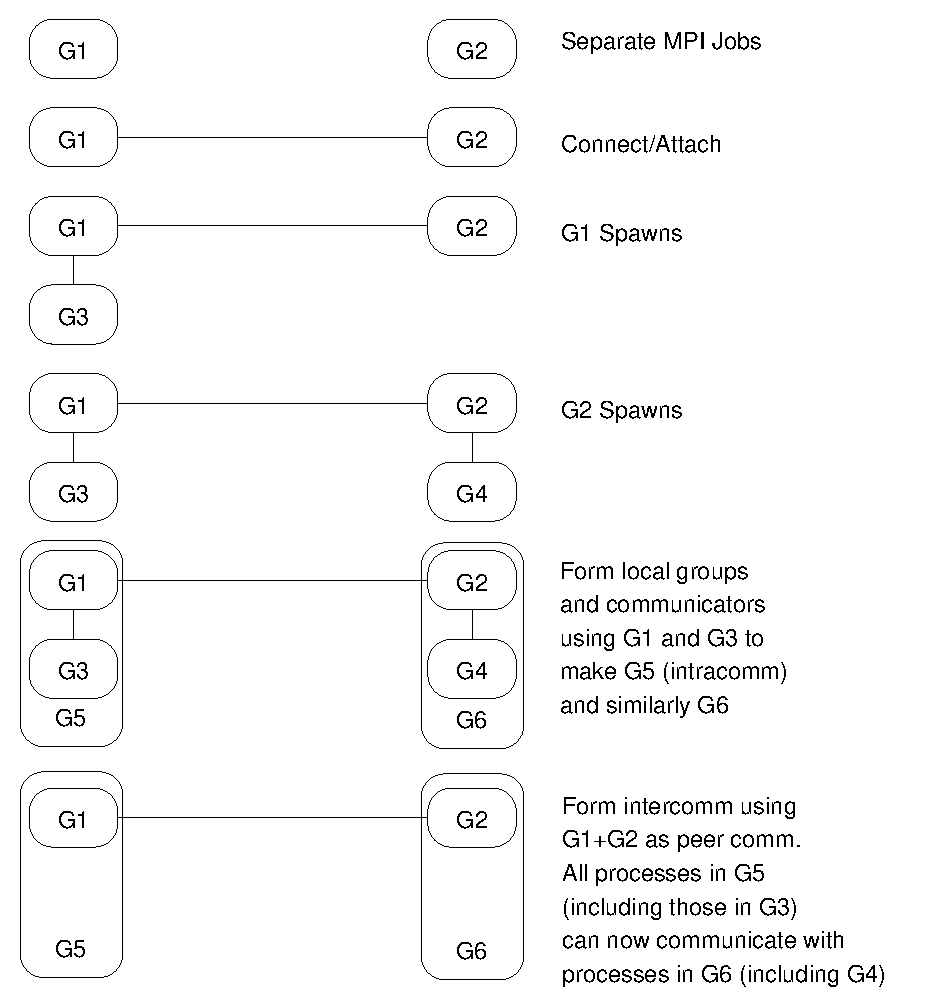
\psfig{file=intercomm.eps,height=4in}}
\caption{Example of MPI process creation and
\mpifunc{MPI_Intercomm_merge}.  Note that the processes in groups G3
and G4 are spawned after the intercommunicator joining groups G1 and
G2 is created.}\label{fig:spawn-ic} 
\end{figure}

The intercommunicator routines should have robust error checking because they
require care and understanding in use and errors are hard to diagnose.  
Errors to check for include inconsistent leaders (all members of the local
group should agree) and overlapping groups (remote and local groups
must not overlap).

Note that this routine is \emph{not} collective in the peer
communicator; that is why a \code{tag} value is required.  That makes
it more difficult to check for consistent leaders between the two
groups, though it could be done tbrough some sort of central registry.
 
\subsubsection{\mpifunc{MPI_INTERCOMM_MERGE}}
Create a new group from the union of the local and remote groups.  Rank 0 in
the group with \code{high == true} communicates with rank 0 in the group with
\code{high == false}.  Once this group is created, call
\mpifunc{MPI_COMM_CREATE} with this group.  

% The following is *not* true, as shown in the figure. 
% Note that all processes in an intercommunicator are already known to the
% local process (see \mpiconst{MPI_INTERCOMM_CREATE}).

\subsubsection{\mpifunc{MPI_COMM_CLONE}}
This is a special C++ function; it behaves similarly to
\mpifunc{MPI_COMM_DUP}, but returns a reference (pointer) to the created
communicator, rather than the communicator itself.  This is necessary because
the C++ binding makes a \code{Comm} an abstract base class, and since
you cannot return an instance of an abstract base class, you can't use
\mpifunc{MPI::Dup} (which returns an instance).  \mpifunc{MPI::Dup}
may only be used on one of the four derived classes.
\mpifunc{MPI::Clone} was provided to give C++ programmers a way to
create a reference to a duplicate of an arbitrary communicator.
Question: should we design an internal dup function so that both
\mpifunc{MPI_COMM_DUP} and the C++ \code{MPI::Comm::Clone} function can use it?

\subsubsection{\mpifunc{MPI_COMM_GET_NAME}}
Return a copy of the \mpids{MPI_Comm}{name} field.  
See \mpifunc{MPI_Type_get_name} for a discussion about Fortran.

Note that unlike the \code{MPI_Type_set_name} and
\code{MPI_Type_get_name} functions, these do not need to initialize
the names of the predefined objects because that is done in
\code{MPI_Init} (there are only two, after all).

Question: MPICH-1 dynamically allocated storage for names rather than
preallocating in the structure.  Do we want to do the same (currently,
we preallocate, which makes all communicator structures larger).

\subsubsection{\mpifunc{MPI_COMM_SET_NAME}}
Set the \mpids{MPI_Comm}{name} field.  Check for valid length.
See \mpifunc{MPI_Type_set_name} for a discussion about Fortran.

\subsection{Point to Point Communication}
\label{sec:pt-2-pt}

The ADI provides a relatively close match to the point-to-point
communication routines.  

\textbf{This section is out-of-date.}

Questions that remain:  Handling of persistent requests.  The ADI
contains memory registration.  Is anything else needed for persistent
requests? 

Should a persistent request simply have a pointer to the active request?  The
request pointer could be null to indicate an inactive persistent request.

Question:  There are a number of flags that we may want to check in order to
drop into a special optimized case.  Should we set things up so that a single
int of flags, where the ``good'' case is a zero bit for each flag, can be
tested with a single compare against zero?

% \subsubsection{\mpidfunc{MPID_Rhcv}}
% This function is not part of MPI but is a critical part of the ADI.
% The choice of implementation depends on the properties of the ADI;
% some are reviewed below.

% \paragraph{Threadedness.}\index{thread overhead!handler
% invocatoin}\index{thread overhead!MPID_Rhcv}In a single-threaded ADI
% implementation, 
% \mpidfunc{MPID_Rhcv} can simply call the appropriate routine to act on
% the object (e.g., deliver a message or inspect a remote queue in
% shared memory).  In an implementation that allows multiple-user
% threads to invoke the ADI routine, \mpidfunc{MPID_Rhcv} must ensure
% that it is thread-safe.  One easy way to do this is to use a lock;
% that is, consider \mpidfunc{MPID_Rhcv} a \emph{synchronized}
% function.  An alternative, particularly when there is a separate
% communication agent (See Section~\ref{sec:comm-agent}), is to have
% \mpidfunc{MPID_Rhcv} enqueue operations on a pending work queue.  This
% operation can sometime be done without a lock (using memory atomic
% operations or load-reservation/store-conditional split operations);
% removing items from the queue can also be done without a lock.

% Questions: do we want a separate send and receive agent in this case?
% The send agent could wait on a condition variable that is set by any
% thread that adds to the queue.  The receiving agent needs to respond
% to events coming from other processes, making the situation somewhat
% asymmetric.  Do we want to have a virtual split, allowing either zero,
% one, or two agents?  

\subsubsection{\mpifunc{MPI_PROBE}}

Call \mpidfunc{MPID_Probe}.  
An implementation of this routine might look something like:

\begin{mmadi}
Look for a match in the unexpected receive queue. 
If no match is found, then wait until another message is receive and check
again.  In a polling, single-threaded implementation, this can simply invoke a
blocking call to wait for incoming messages. 

This routine immediately brings up the problem of how to structure code that
uses multiple threads to achieve good performance when a blocking call is used
by one or more user threads.

Note that in a multithreaded MPI implementation, this must watch for the race
condition of
\begin{verbatim}
     Thread 1                    Thread 2
 Check queue, no match found
                                 Handle incoming unexpected message
 Wait for a message to arrive
\end{verbatim}
Handling this is device-implementation specific.

Consider the following cases:
\begin{enumerate}
\item There is only one thread (e.g., the current \code{ch_p4} case).  In this
  case, after checking the queue, a call that polls the communication agent
  and waits for something to arrive (e.g., with \code{select} for TCP-only
  devices) may be used.  A multimethod device might briefly spin on all
  ``fast'' devices (e.g., shared-memory queues) and then yield the time slice.
\item There is a single thread that acts as the communication agent (see
  Section~\ref{sec:comm-agent}) that is different from the user's thread.
  In this case, the user's thread could pass control to the communication
  agent.  For example, it could use \code{pthread_cond_wait} to wait on the
  communication agent.  The communication agent can use
  \code{pthread_cond_broadcast} to release any user thread that is waiting on
  the communication agent (\code{pthread_cond_signal} may be better if only
  one user thread ever holds the condition variable).
\item There is one communication agent for each method.  For example,
  a TCP method that waits in select for activity on an fd and a thread that
  handles shared memory and may use (in POSIX) \code{sched_yield} after
  spinwaiting (or, in systems that support condition variables shared between
  processes, may use that to wait for an incoming event or message).
  A similar approach may be used here: \code{pthread_cond_broadcast} can be
  used from any method's communication agent thread to release all waiting
  threads. 
\end{enumerate}

%Question: how efficient are the pthread condition wait routines?  Do they spin
%or do they yield the processor to other threads?  This is not specified in the
%POSIX standard; the question is more about the quality of implementation.

The POSIX \code{pthread_cond_wait} has two arguments: a mutex and a condition
variable.  The routine atomically unlocks the mutex and waits for the
condition variable. This suggests, for pthreads, the following solution for
\code{MPID_Request_probe} in the multithreaded cases:
\begin{verbatim}
    while (1) {
        pthread_mutex_lock( &queue_mutex );
        <look through queue>
        if (found) {
            pthread_mutex_unlock( &queue_mutex );
            return;
            }
        else 
            pthread_cond_wait( &queue_mutex, &cond );
    }
\end{verbatim}
In the case of a single user thread, you might want to try
\begin{verbatim}
    <look through queue>
    if (found) return;
    <same code as above>
\end{verbatim}
This is ok as long as the communication agent can't remove items from the
queue.  Unfortunately, cancel does just that.  

In fact, we may want to consider a higher-level abstraction, such as monitors,
which could (usually would) be implemented using locks and condition variables.
\end{mmadi}

\paragraph{Buffered send.}
The buffered send (both blocking and nonblocking) should first use
\mpidfunc{MPID_tBsend} to attempt 
and send the message before implementing the buffer-copying strategy.

Question: should the request needed to implement a buffered send be allocated
from the user-supplied buffer?  The standard suggests so, though it isn't
strictly required.  For example, only the information needed to create
the request could be saved; if no request is available, the bsend
handler can wait until later.

The advantage of not requiring that the request itself be stored in
the Bsend buffer is that the device may want to control who allocates
requests.  Thus, we only store the information needed to get a request
in the bsend buffer.  This has the advantage that it means that the
value of \mpiconst{MPI_BSEND_OVERHEAD} is constant, independent of the
choice of device.

What utility routine should be defined to allocate buffer space from the
user-specified buffer?  How will it be made thread-safe?  What is the
interface to \mpifunc{MPI_REQUEST_FREE}?  How do we ensure that we wait on
pending bsend operations in a polling implementation?  See the file
\file{mpich/src/util/bsendutil2.c} in MPICH-1.  Note that while the buffer is
a global (thread safety warning)\index{thread safety!buffered send},
it can be stored as a local 
\code{static} variable in the file the implements the buffer
management utility routines.

The information on the buffered send buffer is stored in the
\file{bsendutil.c}).  This is an example of keeping the information as
local as possible, since most of the rest of the MPI implementation
need not know about the Bsend.  A finalize callback is used complete
any pending Bsend communication when MPI is exiting.

We need a \mpidfunc{MPIR_Bsend_init} and
\mpidfunc{MPIR_Bsend_finalize} to control the initialization and
finalization of the bsend buffer.  The initialization include
initializing the thread lock used to guard access to the rest of the
structures.   Finalization must ensure that any pending operations
complete (locally); thus the \mpidfunc{MPIR_Bsend_finalize} needs to
be called before any of the routines that free any data structures or state.

The bsend operations are roughly:

Try \mpidfunc{MPID_tBsend}; if it succeeds, done.
Otherwise, find the first block in the buffer that is large enough for
the data, stored as packed with \mpifunc{MPI_Pack}.  
Save: the data, the type of the data (e.g., \code{MPI_PACKED} or some
contiguous type), the count, and the \code{MPI_Request} used to start
an \mpifunc{MPI_Isend} on the data.

As noted above, we must be prepared to save the
communicator, tag, and rank, so that if no request is currently
available, the communication can be deferred until later.  SGI doesn't
do this currently, and as a result, their implementation fails on some
valid MPI programs.

If some bsend operations are deferred pending the availability of a
request, there needs to be some way for the communication agent to
know that it needs to try to send messages once requests become
available.


We take advantage of \mpiconst{MPI_BSEND_OVERHEAD} to ensure that each
block is aligned on a \code{double}.
Note also that the initial buffer itself may not be aligned (the user
can provide a buffer with any alignment; the Bsend code must also take
this into account.  Tests have been added to the test suite to check
for this.
% (question: should we make it a cacheline?)

The fields in the bsend buffer element include
\mpids{MPIR_Bsend_elm}{tag},
\mpids{MPIR_Bsend_elm}{comm},
\mpids{MPIR_Bsend_elm}{rank},
\mpids{MPIR_Bsend_elm}{dtype},
\mpids{MPIR_Bsend_elm}{count}, and 
\mpids{MPIR_Bsend_elm}{request}, as well as \mpids{MPIR_Bsend_elm}{next}.

The bsend buffer itself is described by
\mpids{MPIR_Bsend_buffer}{buffer}, \mpids{MPIR_Bsend_buffer}{size},
\mpids{MPIR_Bsend_buffer}{head}, \mpids{MPIR_Bsend_buffer}{tail}, and
\mpids{MPIR_Bsend_buffer}{pending}.  The value of \code{tail} points
to the first free byte and \code{head} points to the first used byte,
or to \code{tail} if the buffer is empty.

Question: for the nonblocking versions, in principle, we could wait to
copy into the buffer until the wait/test.  Maybe in 2008.

% An implementation of \mpidfunc{MPID_tBsend} might look like:

% Check message size.  
% If not within eager limit, return false
% If flow control allows, send and return true, 
% else return false

% Note that the flow control check may require a lock so that another
% thread doesn't also try to send and change the flow control state.

\begin{figure}
\centerline{\includegraphics{bsend.eps}}
\caption{Explanation of \texttt{size} and \texttt{total_size} fields in the
\texttt{BsendData_t} header.  In (a), an unallocated element, pointed at by
\texttt{p} is shown.  The difference between the two sizes is just the size of
the header.  In (b), an allocated element is shown.  Here, the \texttt{size}
is smaller, reflecting the need to align the \texttt{BsendData_t} header on a
suitable boundary.}
\label{fig:bsend-buffers}
\end{figure}

\subsubsection{\mpifunc{MPI_IBSEND}}
See Buffered send.

\subsubsection{\mpifunc{MPI_BSEND}}
See Buffered send.

\subsubsection{\mpifunc{MPI_BSEND_INIT}}
Remark:  Note that this should not reserve space in the buffer for the
data.  That step should be performed when the communication is started
with \code{MPI_Start} or \code{MPI_Startall}.

\subsubsection{\mpifunc{MPI_BUFFER_ATTACH}}

If a buffer is already attached, return error.
Otherwise, attach the designated buffer and initialize the buffer as empty.
The buffer is organized as a circular buffer as described in the model
implementation of buffered mode in the MPI standard.


\subsubsection{\mpifunc{MPI_BUFFER_DETACH}}
Buffer detach must first wait for all operations to complete before
returning.  
In order to catch race conditions in a multi-threaded environment, 
\code{MPI_Buffer_detach} should set a flag on the buffer on entrance; all
buffered send operations should check this value before proceeding, generating
a \mpiconst{MPI_ERR_OTHER} class of type \code{THREAD_RACE} if the flag is
set.

\subsubsection{\mpifunc{MPI_CANCEL}}
Check the kind of the request:
\begin{itemize}
\item Inactive persistent.  Return error.
\item Active persistent.  Handle as a non-persistent request of the same type.
\item Receive.  Call \mpidfunc{MPID_Cancel_recv}.  If already complete
or in progress, cancel fails.   
% \begin{core} 
% Otherwise, remove request from receive queue (atomically).  In many
% ADIs, this is a local operation.  However, some systems may require
% logic similar to the send branch (this is the speculative receive
% case, where information on a receive with a designated source is sent
% directly to the sender).

% Question: The check-and-remove must be done atomically.  This needs a
% variation of the find-or-allocate that performs a find-and-remove.

% \end{core}
\item Send. Call \mpidfunc{MPID_Cancel_send}.  If already complete or
in progress, cancel fails. 
% \begin{core} 
% Otherwise use \mpidfunc{MPID_Rhcv} to send a cancel
% request (\mpidconst{MPID_Hid_cancel}).  The cancel operation must wait for a
% acknowledgement that 
% indicates whether the cancel succeeded or failed.  

% Question: How is this wait managed?  For a polling implementation, should this
% use some (possibly higher latency) alternate communication path (e.g., a
% \code{SIGIO} handler for TCP or \code{SIGUSR1} for shared memory)?

% Again, the check and send if not in progress must be atomic.  
% Essentially, the cancel matches the send request in the queue and
% marks it as satisfied.

% How is the send identified?  By the same request id that is used by
% the \mpidconst{MPID_Hid_ok_to_send}?  

% Note that if we receive an ok-to-send on this request, it means that
% the send cancel has failed.  No separate negative-ack is required.
% That is, in the communication agent, if the send is in progress, the
% cancel request may be discarded without further action, at least in
% cases where a separate acknowledgement is required to initiate the
% data transfer described by a send.
% \end{core}
\end{itemize}

Remark: We should have an attribute that indicates that there
are no send-cancels.  Handling send-cancel is the only part of MPI-1
that requires that a communication agent runs even if no MPI calls are
made by a process.  Question: what is the keyval of this attribute?

Remark: there was some discussion in MPICH-1 that send-cancel required more
care that described here (including a time-stamp on requests to ensure
that the correct request was cancelled.  Here's the situation
\begin{verbatim}
     process 0                             process 1
   thread 0    thread 1                
   isend 
   cancel                                   irecv (matches isend)
             <------- ok-to-send  -------<
   send matched, removed
               isend(same request)
                                            isend arrives
                                            cancel arrives (late)
\end{verbatim}
At the end of this, the cancel matches the second isend even though it
should only match the first.  However, to avoid this, we need only
wait until we receive a response from the destination process about
whether the cancel succeeded or not before freeing the request.  To
accomplish this, we need only increment the reference count on the
request when canceling it, decrementing the reference count on the
response from the destination process.

% To avoid this, we only need a sequence
% number on the messages; we need this anyway for supporting profiling.
% Another alternative is to manage the list of available requests as a
% FIFO rather than LIFO queue; in that case, there's very little chance
% that the same request woul be used soon enough to cause any problems.  
% Other solutions can be used; if the communication is handled by a
% single thread, the fact that the request is not made available again
% until the cancel is known to either have succeeded or failed
% guarantees that no mismatch can occur.

\subsubsection{\mpifunc{MPI_IPROBE}}
\mpidfunc{MPID_Request_iprobe}
% \begin{mmadi}
% This is the same code as \mpidfunc{MPID_Request_recv_FOA}, but without
% the allocation if no matching request is found.  See
% \mpifunc{MPI_Probe} for additional discussion; \mpifunc{MPI_Iprobe},
% of course, does not block.
% \end{mmadi}


\subsubsection{\mpifunc{MPI_IRECV}}
\begin{adi3}
\mpidfunc{MPID_Irecv}
% \begin{mmadi}
% \mpidfunc{MPID_Segment}\\
% \mpidfunc{MPID_Request_recv_FOA}\\
% \mpidfunc{MPID_Stream_irecv}
% \begin{core}
% This should ensure that any polling call is made.  Question: what is
% the interface with the communication agent?  Note that the agent will
% arrange the actual data transfer.  In a multithreaded case, the
% calling (user) thread only enqueues the request.

% The implementation of \mpidfunc{MPID_Request_recv_FOA} might include:
% \begin{mmadi}
% Determine source.  If a specific source, find or add (atomically) to
% the queue for that method. 
% If \mpiconst{MPI_ANY_SOURCE}, then 
%     lock common queue
%     find or add (atomially) to each method's queue; stop if there is a
%     match
%     add to common queue
%     unlock common queue.
% \end{mmadi}

% \end{core}
% \end{mmadi}
\end{adi3}

\subsubsection{\mpifunc{MPI_IRSEND}}
Call \mpidfunc{MPID_Irsend}.
% Is this the same as \code{MPI_ISEND}, but with the ready mode set?  Or is
% there a separate routine that exploits the ready nature of the operation?
% Special note: we should be able to report an error when a ready send is not
% matched by a posted receive.  This requires a bit for ready mode in the
% \mpidconst{MPID_Hid_short} and \mpidconst{MPID_Hid_request_to_send}; perhaps a
% \mpids{MPID_Hid_short}{is_ready}\index{MPID_Hid_request_to_send!is_ready}. 

\subsubsection{\mpifunc{MPI_ISEND}}
\begin{adi3}
\mpidfunc{MPID_Isend}
% \begin{mmadi}
% \mpidfunc{MPID_Segment}\\
% \mpidfunc{MPID_Request_send_FOA}\\
% \mpidfunc{MPID_Stream_isend}
% \begin{core}
% If the message is small in total size and flow control allows it, send
% the data with \mpidconst{MPID_Hid_short} using \mpidfunc{MPID_Rhcv}.
% Otherwise, send a \mpidconst{MPID_Hid_request_to_send} with
% \mpidfunc{MPID_Rhcv}.  
% \end{core}
% \begin{via}
% Attempt to register the source memory so that direct memory operations may be
% used on it.  If this is not possible (e.g., no more memory can be pinned),
% then copy to some preallocated space.
% \end{via}
% \end{mmadi}
\end{adi3}

% Question: do we want a special case for short messages that reduces
% overhead by indicating that the message is completed?  Note that for
% any operation that is not complete, we must ensure that the related
% objects, such as datatypes and communicators, are marked as in use (by
% incrementing their \mpids{MPI_Comm}{ref_count}.  This is not needed if
% the operation is already complete, and eliminating these steps may be
% important for reducing the latency of short messages (particularly
% since, in the multi-threaded case, updating the reference count
% requires a write and, for objects being used by several threads, a
% cache miss.

%% The following is commented out because the MPID layer is
%% responsible for updating the reference counts
Another special case is the predefined, permanent objects.  Should the
\mpids{MPI_Datatype}{ref_count} be updated for those objects (answer:
no)?  Is the branch (we've already loaded the object identifier)
faster than the 
load/increment/store?  

\subsubsection{\mpifunc{MPI_ISSEND}}
Same as \code{MPI_ISEND}, but with the synchronous mode set.  

% \begin{core}
% For all sizes, use \mpidconst{MPID_Hid_request_to_send} with
% \mpidfunc{MPID_Rhcv}.  Note that this includes messages of size zero.
% In the absence of a speculative receive, this will never complete
% before the routine an exit.

% \end{core}
% Note that an alternate approach is possible for short messages that uses
% \mpidconst{MPID_Hid_short} but requires an acknowledgement when the message is
% matched at the destination.  At least for now, we don't plan to implement this
% approach (it was used in MPICH/ADI-1, but was not really worth the effort). 

\subsubsection{\mpifunc{MPI_RECV}}
Call \mpidfunc{MPID_Recv}.  Note that this routine is permitted to return a
\mpidconst{MPI_Request}; in that case, we must wait on the request.

% This can simply be \code{MPI_IRECV} followed by an \code{MPI_WAIT}.  However,
% we might want to let the partner (matching sender) know that this is blocking
% a thread or process.  

% Note that an early version of MPICH waited for a specific tag,
% context-id, and source tuple.  This sped up the process of matching
% against the message queue (incoming messages were first matched
% against that tuple), but it isn't correct if the queue already
% contains entries with wild cards (e.g., \mpiconst{MPI_ANY_SOURCE}).

\subsubsection{\mpifunc{MPI_RECV_INIT}}

Call \mpidfunc{MPID_Recv_init} to create a persistent request and save
the message 
parameters (\mpids{MPI_Request(persistent)}{communicator}, 
\mpids{MPI_Request(persistent)}{tag}, \mpids{MPI_Request(persistent)}{source_rank}, 
\mpids{MPI_Request(persistent)}{datatype},
\mpids{MPI_Request(persistent)}{buffer}, and
\mpids{MPI_Request(persistent)}{count}). 

%% Now part of the persistent request code
% Call \code{MPID_Memory_register} for either the buffer or a created segment
% that will be used for receiving the data.  

Note that a persistent request is not like an
\mpidconst{MPID_Request}; rather, it only contains enough information
to identify it as a persistent request and a pointer to a normal
\mpidconst{MPID_Request}.  In fact, the pointer to the request can be
used to indicate whether the persistent request is active, rather than
using a separate field.  This field could be
\mpids{MPI_Request}{active_request}.


Note that \mpidfunc{MPID_Memory_register} must fix both the physical
memory and the virtual to physical mapping, so that both any
peripheral device (such as a network card that implements VIA) and the
process will both access the same locations.  Apparently, Linux
doesn't provide this service, and it must be emulated by restricting
the behavior of \code{malloc}!

\subsubsection{\mpifunc{MPI_REQUEST_GET_STATUS}}
Extract the status data from the request.
This requires either an \mpidfunc{MPID_Request_get_status} or clearly defined
status elements in the \mpidfunc{MPID_Request}.  The current choice is
to use the \mpids{MPID_Request}{status} field in \mpidconst{MPID_Request}.

% Question: do we want to use something besides status?  If we do use
% status, it should be the \mpids{MPI_Request}{status} field.

\subsubsection{\mpifunc{MPI_REQUEST_FREE}}
\begin{adi3}\mpidfunc{MPID_Request_free}
%\begin{mmadi}
%\begin{core}
%\end{core}
%\end{mmadi}
\end{adi3}
Question: Who handles persistent or user-defined requests?

Note that this is not the same as cancelling a request.  
A request that is freed must still complete.  Thus, the request needs
a reference count (\mpids{MPI_Request}{ref_count}) that must be
checked when the related communication 
completes.  If the count is zero, there will be no \code{MPI_Wait}
etc. call, and the request data strucutre must be recovered.  A
polling device that expects a wait or test call may need to maintain a
list of freed but not completed requests and effectively call
\mpidfunc{MPID_Testsome} on that list.  See Section~\ref{sec:comm-agent}.

\subsubsection{\mpifunc{MPI_RSEND}}
Like \mpifunc{MPI_Send}, but with the ready mode.  This is a bit in
the message header (at least when full debugging is enabled) that can
be checked at the destination to detect an erroneous use of
\mpifunc{MPI_RSEND} (no matching receive).

\subsubsection{\mpifunc{MPI_RSEND_INIT}}
See \mpifunc{MPI_RECV_INIT}.

\subsubsection{\mpifunc{MPI_SEND}}
See \mpifunc{MPI_ISEND}.  This could simply be isend followed by wait.

Question: do we want to indicate to the receiver that this is a
blocking send?  For example, that would suggest a higher priority in
handling the operation, since a single threaded source process may be
blocked on this operation.

\subsubsection{\mpifunc{MPI_SENDRECV}}
Question: If the source and destination are the same, is there anything
special that we want to do?  Note that this routine matches communication from
any point-to-point operation, not just other sendrecv calls.  
Simply use \mpifunc{MPI_Isend}, \mpifunc{MPI_Irecv}, and
\mpifunc{MPI_Waitall}. 

Note that in the case of a rendezvous exchange where the data is sent
in a number of blocks, an exchange can be handled more efficiently
that two independent isend/irecv pairs, as shown in Figure~\ref{fig:sendrecv}.
\begin{figure}
\centerline{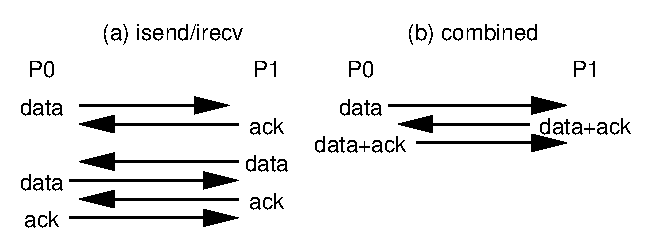
\psfig{file=sendrecv.eps,width=4in}}
% (temporary figure)
%     (a) isend/irecv                           (b) combined
%   p0                  p1                p0                   p1
%   data ------->                        data -------------->
%        <-----------   ack                   <-------------- data+ack
%        <-----------  data              data+ack ------------>
%   data ------------>
%   ack  ------------>
% \end{verbatim}
\caption{Two sendrecv scenarios}\label{fig:sendrecv}
\end{figure}
Question: do we want to allow ok-to-send acks to be piggy-backed onto
an ongoing data stream?  Once a data stream starts, we can record that
it is ongoing; any ack to that partner can be added to the ongoing
stream.  If no communication is pending, the ack can be sent
immediately.

Note that since \mpifunc{MPI_Sendrecv} can match other MPI
communication calls, such as \mpifunc{MPI_Send} and
\mpifunc{MPI_Irecv}, we cannot depend on \mpifunc{MPI_Sendrecv} to
give us enough information to decide whether to piggyback acks on a
data stream.

\subsubsection{\mpifunc{MPI_SENDRECV_REPLACE}}
% Question: Should this use the segment code to bound the memory buffer that
% must be allocated for the replacement?
% \begin{adi3}
% \mpidfunc{MPID_Segment}, \mpidfunc{MPID_Stream_irecv}, and
% \mpidfunc{MPID_Stream_isend}. 
% \end{adi3}

\subsubsection{\mpifunc{MPI_SEND_INIT}}
Call \mpidfunc{MPID_Send_init}.  See \mpifunc{MPI_Recv_init} for more
details. 

\subsubsection{\mpifunc{MPI_SSEND}}
Like \mpifunc{MPI_Send}, but with the synchronous mode.

\subsubsection{\mpifunc{MPI_SSEND_INIT}}
See \mpifunc{MPI_RECV_INIT}.

\subsubsection{\mpifunc{MPI_START}}
This just calls \mpifunc{MPID_Startall} with a single request.  
% Note that
% errors must indicate that the error occurred in \code{MPI_START}, not
% \code{MPI_STARTALL}.  

\subsubsection{\mpifunc{MPI_STARTALL}}
Do we want startall to allow for some scheduling of the operations?  For
example, it could start the ``furthest away'' first.  It could also batch
operations.
% (see the paper on improving TCP performance \cite{??}).  
If so, we need an \mpidfunc{MPID_Startall}.

Should each of the individual persistent routines provide an internal
routine that is used to start the operation?
These can simply call the related non-persistent routine using the fields from
the persistent request (e.g., \mpids{MPI_Request(persistent)}{communicator})
and storing the new request in the \mpids{MPI_Request(persistent)}{request}
field. 

Note that generalized requests are not started with \mpifunc{MPI_START}; i.e.,
there is no persistent generalized request.

\subsubsection{\mpifunc{MPI_STATUS_SET_CANCELLED}}
Where are the values defined for indicating cancelled message?
A \mpidconst{MPID_COUNT_MSG_CANCELLED} for the count field in the
status?
(We shouldn't use the \mpids{MPI_Status}{MPI_TAG} field of
\mpiconst{MPI_Status} because that field is visible to the user.)
MPICH-1 currently sets the \code{MPI_TAG} field to \code{MPIR_MSG_CANCELLED}.

\subsubsection{Point-to-point completion functions}
There are several special kinds of requests that require special handling by
all of the completion (e.g., \code{MPI_Test} and \code{MPI_Waitany})
functions. 

Generalized requests:  On completion, invoke the
\mpids{MPI_Request(generalized)}{free_fn}. 

Persistent requests: The actual request is the
\mpids{MPI_Request(persistent)}{active_request} in the
\mpidconst{MPID_Request} structure.

Rather than have separate routines for each of the MPI completion
functions, we instead use the \mpids{MPI_Request}{busy} flag in the
\mpiconst{MPID_Request}.  In the case of a completed request, this
eliminates the need to call an additional function.  Otherwise, the
MPI code must make the appropriate progress engine calls.  For
example, \mpifunc{MPI_Wait} looks something like this:
\begin{verbatim}
    MPI_Wait( ... )
    {
        while (request->busy) {
            MPID_Progress_start( );   // Notes that we are about to
                                      // check ready flags.  No busy 
                                      // flags will be cleared
            if (request->busy) {
                MPID_Progress_wait();
            }
            else {
                MPID_Progress_end();
            }
        }
        if (request->type & REQUEST_IS_RECV && status) {
            *status = request->status;
        }
    }
\end{verbatim}
The reason for the \mpidfunc{MPID_Progress_start} and the other
progress routines becomes clear when you consider
\mpifunc{MPI_Waitsome}.
Note that there are no explicit thread locks in this example.  

\paragraph{Previous Discussion.}
(This text is still true but represents a different direction that we
are no longer planning to take.)

The two most basic routines are \mpifunc{MPI_Testany} and
\mpifunc{MPI_Waitany} in the sense that all of the other operations
can be built from these.  For example:
\begin{description}
\item[\mpifunc{MPI_Wait}]\mpifunc{MPI_Waitany}
\item[\mpifunc{MPI_Waitsome}]\mpifunc{MPI_Waitany} followed by
\mpifunc{MPI_Testsome} (or \mpifunc{MPI_Testany} until flag is false).
Note that without the \mpifunc{MPI_Testsome} 
call, the requirements of \mpifunc{MPI_Waitsome} won't be met; in
particular, the \mpifunc{MPI_Testsome} is needed to allow
\mpifunc{MPI_Waitsome} to provide fairness (indicate \emph{all}
requests that are ready).
\item[\mpifunc{MPI_Waitall}]\mpifunc{MPI_Waitany} until all non-null
requests have completed.
\item[\mpifunc{MPI_Test}]\mpifunc{MPI_Testany}
\item[\mpifunc{MPI_Testsome}]\mpifunc{MPI_Testany} until flag returns
false.
\item[\mpifunc{MPI_Testall}]\mpifunc{MPI_Test} for each request.
\end{description}
These are not necessarily the best implementations of the eight
completion functions, but they do provide reasonable implementations
as long as the number of requests provided to the completion function
is not too large (since some of the algorithms above have complexity
proportional to the square of the number of requests).

% Question:  Should we define \mpidfunc{MPID_Testany} and
% \mpidfunc{MPID_Waitany} instead of the \mpidfunc{MPID_Testsome} and
% \mpidfunc{MPID_Waitsome} routines?

\subsubsection{\mpifunc{MPI_TEST}}
Check the \mpids{MPI_Request}{busy} flag.  Call
\mpidfunc{MPID_Progress_poke} and check again if
\mpids{MPI_Request}{busy} is true.

\subsubsection{\mpifunc{MPI_TESTALL}}
Like \mpifunc{MPI_Test}, but for all requests.  However, call
\mpidfunc{MPID_Progress_poke} \emph{first}, since it is likely that
not all requests will already be completed.

\subsubsection{\mpifunc{MPI_TESTANY}}
Like \mpifunc{MPI_Testall}, but stop on the first completed request.

% Call \mpidfunc{MPID_Testsome} on each request, one at a time.

% Question: do we want something better?  Can we subdivide
% \mpidfunc{MPID_Testsome} into smaller building blocks from which we
% can build the four test routines without dropping down to an
% \mpidfunc{MPID_Test}?  For example, the closest match to \code{select} is to
% implement xxxsome, for advancing the state/completing operations, but decide
% how to update/record the requests that have completed based on whether the
% call is implementing the any, all, or some version.

\subsubsection{\mpifunc{MPI_TESTSOME}}
Like \mpifunc{MPI_Testall}.

\subsubsection{\mpifunc{MPI_TEST_CANCELLED}}
This uses the status field, specifically the
\mpids{MPI_Status}{MPI_TAG} field, in a request to test for a cancelled
message.  See the discussion under
\mpifunc{MPI_STATUS_SET_CANCELLED}.  We need to decide.

\subsubsection{\mpifunc{MPI_WAIT}}
As described above under point-to-point completion functions.

\subsubsection{\mpifunc{MPI_WAITALL}}
Like \mpifunc{MPI_Testall}, but must wait until all requests are complete.

\subsubsection{\mpifunc{MPI_WAITANY}}
See \mpifunc{MPI_Testany}.

\subsubsection{\mpifunc{MPI_WAITSOME}}
See \mpifunc{MPI_Testsome}.

\subsection{Communication Agent}
\label{sec:comm-agent}
All implementations require some sort of communication agent.  This agent
handles the delivery of data as described by \mpifunc{MPI_Recv} and
\mpifunc{MPI_Irecv}, RMA operations that require action at the target (such as
handling complex datatypes and for two-sided communication layers),
progress for nonblocking sends, and more
subtle operations such as cancelling of nonblocking sends.  This agent may be
invoked explicitly (a polling interface) or implicitly (e.g., in response to
an I/O interrupt or a thread-schedule event).  

Note that the communication agent is very device-specific.  See the
discussion of the agents for the particular devices.
% \begin{tcp}
% Receive a message header.  This is a message sent with \mpidfunc{MPID_Rhcv},
% and the header is one of the \mpidconst{MPID_Hid_xxx_t} structures.
% Based on the header type, invoke the appropriate processing routine (there
% should be one for each header type, such as
% \mpidfunc{MPID_Hid_xxx_method}). 

% Still to do:  List the detailed behavior of head message type.
% \begin{description}
% \item[\mpidconst{MPID_Hid_short}.]
% Call \mpidfunc{MPID_Request_recv_FOA}.  If found, transfer data using
% \mpidfunc{MPID_Unpack}.  Otherwise, save data (transfer with \code{memcpy}) in
% message buffer area.  Update flow control.
% Special case: If ready-message bit is set and no matching message
% exists, use \mpidconst{MPID_Hid_control} to return a remote error
% indication.
% Fields include \mpids{MPID_Hid_short}{size},
% \mpids{MPID_Hid_short}{tag}, \mpids{MPID_Hid_short}{context_id},
% \mpids{MPID_Hid_short}{source_rank}, and
% \mpids{MPID_Hid_short}{data}.  It may also include
% \mpids{MPID_Hid_short}{type_sig}, containing the shortened type
% signagure, and \mpids{MPID_Hid_short}{flags}, containing various flags
% (such as \mpidconst{MPID_READY_SEND}).  Heterogeneous systems must
% also contain \mpids{MPID_Hid_short}{data_format}, which may include
% the rank of the process that packed the data for data sent with
% \mpiconst{MPI_PACKED} (see Section~\ref{sec:mpi-unpack}).

% \item[\mpidconst{MPID_Hid_request_to_send}.]
% Call \mpidfunc{MPID_Request_recv_FOA}.  If found, reply with
% \mpidconst{MPID_Hid_ok_to_send} sent with \mpidfunc{MPID_Rhcv}.  Otherwise,
% store message id in newly allocated request and mark request as ready
% for use.  
% Fields include \mpids{MPID_Hid_request_to_send}{size},
% \mpids{MPID_Hid_request_to_send}{tag},
% \mpids{MPID_Hid_request_to_send}{context_id}, 
% \mpids{MPID_Hid_request_to_send}{source_rank}, and a
% \mpids{MPID_Hid_request_to_send}{request_id}, which is used to
% identify this operation to the sender when it is acknowledged.  
% It may also include
% \mpids{MPID_Hid_request_to_send}{type_sig}, containing the
% request_to_sendened type 
% signagure, and \mpids{MPID_Hid_request_to_send}{flags}, containing
% various flags 
% (such as \mpidconst{MPID_READY_SEND}).  Heterogeneous systems must
% also contain \mpids{MPID_Hid_request_to_send}{data_format}, which may include
% the rank of the process that packed the data for data sent with
% \mpiconst{MPI_PACKED} (see Section~\ref{sec:mpi-unpack}).

% Question: In order to implement the store and forward stream
% operation, should there be a ``disposition'' field that indicates what
% to do with the raw (pre-unpacked) data?

% \item[\mpidconst{MPID_Hid_ok_to_send}.]Send the requested data back
% with a header of \mpidconst{MPID_Hid_data}.  Note that this may be
% only a subset of the full data.  That is, a long message may be sent
% as multiple pieces.  Each piece requires an \mpidconst{MPID_Hid_data}
% header.
% Fields include \mpids{MPID_Hid_ok_to_send}{request_id} and
% \mpids{MPID_Hid_ok_to_send}{recv_id}, which is used to identify the
% data in \mpidconst{MPID_Hid_data}.  

% Question: do we also want to return a maximum data length to indicate
% the maximum amount of data that should be returned?

% \item[\mpidconst{MPID_Hid_data}.]Is this just \mpidconst{MPID_Hid_put}
% where the address has been sent with \mpidconst{MPID_Hid_ok_to_send}?
% The fields in this structure include \mpids{MPID_Hid_data}{recv_id},
% \mpids{MPID_Hid_data}{size}, and \mpids{MPID_Hid_data}{data}.  We may
% also want to include the corresponding
% \mpids{MPID_Hid_data}{request_id} to simplify the process of handling
% the case wheere the data is delivered in several parts.

% \item[\mpidconst{MPID_Hid_cancel}.]Attempt to access a previous
% request.  If unmatched, remove it and return a success
% \mpidconst{MPID_Hid_cancel_ack} using \mpidfunc{MPID_Rhcv}.
% Otherwise, return a failure and leave the request as unchanged.
% The fields here include \mpids{MPID_Hid_cancel}{request_id} (matching
% a \mpidconst{MPID_Hid_request_to_send}).

% \item[\mpidconst{MPID_Hid_cancel_ack}.]Set the cancel success/failure
% field of the indicated request.  Question: Do requests need a separate
% field to indicate failed cancel, or can \mpifunc{MPI_Test_cancelled}
% return failure if it doesn't find success (e.g., do we need to
% distinquish between cancel attempted and failed and never attempted?
% Question: Should there be a single cancel type with an operation
% subfield that combines \mpidconst{MPID_Hid_cancel} and
% \mpidconst{MPID_Hid_cancel_ack}?
% The fields here include \mpids{MPID_Hid_cancel_ack}{request_id} and
% \mpids{MPID_Hid_cancel_ack}{flag}, indicating success or failure.

% Question: do we ever need the failure, since that will mean that a
% \mpidconst{MPID_Hid_ok_to_send} was generated for the request?

% \item[\mpidconst{MPID_Hid_lock_op}.]Manipulate a lock on the indicated
% window object.  The operation are lock, lock-exclusive, unlock, and
% lock-grant (we don't need an unlock-grant).  The window object is
% specified by the window object id (previous set as part of the
% \mpifunc{MPI_Win_create} step).
% Fields include \mpids{MPID_Hid_lock_op}{source_rank},
% \mpids{MPID_Hid_lock_op}{window_id}, and
% \mpids{MPID_Hid_lock_op}{flags}, which indicate whether this is a lock
% or unlock, and whether it is exclusive or not.

% \item[\mpidconst{MPID_Hid_win_count_op}.]Modify one of the local window
% start/complete counters (see \mpifunc{MPI_Win_start}).  

% \item[\mpidconst{MPID_Hid_put}.]Emulate a put operation.  The handler
% contains the offset of the destination and window object id, as well
% as the size.  
% Question: should we have the sender convert the offset to an address?
% Question: does this assume contiguous data?  If it does, do we want a
% strided access version?
% Fields include \mpids{MPID_Hid_put}{offset},
% \mpids{MPID_Hid_put}{window_id}, \mpids{MPID_Hid_put}{datatype_id},
% and \mpids{MPID_Hid_put}{count}.

% Question: do we really want a stream version of this instead?  How do
% we implement streams without it?

% \item[\mpidconst{MPID_Hid_accumulate}.]Emulate an accumulate
% operation.  Much like \mpidconst{MPID_Hid_put}.

% \item[\mpidconst{MPID_Hid_get}.]Like \mpidconst{MPID_Hid_put}, but for
% the get operation.  Question: Should there be a single RMA type, with
% put, get, and accumulate as separate subtypes?

% \item[\mpidconst{MPID_Hid_flow}.]Flow control.  This sends an update
% about the free resources of the sender.  Should a variation of this
% request an update?  Also, do we want to a version that request more or
% less resources for buffering?  Do we want to piggyback flow control
% information on all headers?  E.g., we could use a single signed char
% (byte) to update the number of data blocks in use; this would reduce
% the number of flow-control only messages.

% \item[\mpidconst{MPID_Hid_datatype_desc}.]Cache a datatype description
% to be used in RMA operations.  This is similar to a
% \mpidconst{MPID_Hid_request_to_send}, including the need to use a
% rendezvous to send complex and lengthy datatypes (e.g., indexed
% types).
% Question: As for \mpidconst{MPID_Hid_lock_op}, should there be a
% single type with subfields?  

% \item[\mpidconst{MPID_Hid_control}.]This is a general-purpose control
% message.  For example, this could be used to implement an abort,
% disconnect, deadlock detection, remote error indication (e.g., a ready
% send that was not matched), and orderly exit.
% \end{description}

% Questions and comments:

% The communication agent for methods based on network read/write
% operations such as TCP should probably use a buffered read to reduce
% the number of system 
% calls.  The buffering code should be able to switch to direct read when a
% large amount of data is being moved (by emptying the buffer and then switching
% to direct read).  

% How is flow control handled?  Should flow control be bundled with the buffered
% read/write logic?

% Are there separate stream operations?  Are there stream operations
% instead of the \mpidconst{MPID_Hid_request_to_send} etc. operations?
% \end{tcp}

% \begin{shmem}
% Is this the same as \tcpname, but with slightly different message
% types?
% Where are there differences?  For example, should datatypes be stored
% in shared memory, thus eliminating the
% \mpidconst{MPID_Hid_datatype_desc}?  If so, how does the device ensure
% that the datatype code places everything in shared memory (e.g.,
% \mpifunc{MPI_TYPE_CREATE_INDEXED} cannot use \code{malloc} to save the
% index arrays)?  Should the lock/unlock operations
% be direct rather than using \mpidconst{MPID_Hid_lock_op}?
% If the message queues are stored in shared memory, how does that
% change the various routines?  For example, does a \shmemname\ device not
% use \mpidconst{MPID_Hid_short}, using instead direct access to shared
% memory so as to reduce the latency of short messages?

% Note that since the assumption is that only some memory is shared, it
% isn't possible to implement most message operations without using a
% communication agent at the destination to implement the transfer of
% data into user-defined buffers that are not in shared memory.

% Question:  Do we want a separate case for systems that can share all
% of process memory (Windows and Linux)?
% \end{shmem}

% \begin{via}
% Like \tcpname, except some data can be transfered without the agent
% (remote read and write (get/put) operations).
% \end{via}

% subsection collective communication and computation; contains the
% discussion.  The description of each individual routine remains in the
% mpich2.tex file for now.
\subsection{Collective Communication and Computation}
\label{sec:collective-comm}

One of the major changes in MPICH2 is in the implementation of the
collective routines.  The MPICH2 implementation will exploit
pipelining and store and forward algorithms; these are supported by
the XFER interface. 
%\code{MPID_Stream_xxx} routines.  

Since each system may have some feature that provides for even faster
implementation of the collective routines, it will be possible to
substitute a system-specific implementation for any of the collective
routines.  The purpose of the implementations provided with MPICH is
to provide a level of performance that will be adequate
for many users.  

The $\alpha$-tree approach described in
\cite{bern:mpi-collective:hpcn99} should be considered; this is a
simple variation on the binomial tree approach used in the MPICH
implementations of many of the collective routines.  We will consider
combining this with the pipelining and scatter/gather approaches
championed by van de Geijn (\cite{vandegeijn} isn't quite the right
reference but it will do for now).

\subsubsection{Reduction functions}
The reduction functions must use the \code{restrict}\index{restrict} qualifier.

Each reduction operation (e.g., \code{MPI_SUM}) has a corresponding
implementation (e.g., \code{MPIR_Sum}) and is placed in a separate file (e.g.,
\file{opsum.c}.  Each of these must be careful to conditionally include the
Fortran datatypes and Fortran logical operations (see
Section~\ref{sec:fortran}).

Some reduction functions are not defined on a particular datatype.  To
indicate errors, the routine \code{MPID_Op_set_error} is called.
The MPI reduction routine (reduce, allreduce, scan, exscan, and reducescatter)
checks this with \code{MPID_Op_get_error}.  In order to ensure that
separate threads manage their own error flags for reductions, there is
an \mpids{MPIR_PerThread}{op_error} field in the per-thread data
structure.

% An implementation of this might be 
% \begin{verbatim}
% #ifdef MPID_HAS_THREADS
% /* Use thread private storage for the error value.  Allocate on demand */
% extern int MPID_Op_error_key;
% void MPID_Op_error_delete( void *val ) { if (val) free(val); }
% #define MPID_Op_error_init \
%     pthread_key_create( &MPID_Op_error_key, MPID_Op_error_delete )
% #define MPID_Op_error_finalize \
%     pthread_key_delete( MPID_Op_error_key )
% #define MPID_Op_set_error(err) {\
%  int *e = (int*)pthread_get_specific(MPID_Op_error_key); \
%  if (!e) { e = (int*)malloc(sizeof(int));\
%            pthread_set_specific( MPID_Op_error_key, e );}\
%  *e = err; }
% #define MPID_Op_get_error(err_p) \
%     *err_p = *(int*)pthread_get_specific(MPID_Op_error_key)
% #else
% #extern int MPID_Op_error;
% #define MPID_Op_error_init
% #define MPID_Op_error_finalize
% #define MPID_Op_set_error(err) MPID_Op_error = err
% #define MPID_Op_get_error(err_p)  *(err_p)=  MPID_Op_error
% #endif
% \end{verbatim}


\subsubsection{Code Structure for the Implementation of the Collective
  functions} 

The MPICH code uses one gigantic file, \file{intraops.c}, to provide a
generic implementation of each collective operation.  Each
communicator has a structure of pointers to functions.  Unless
otherwise set, each communicator points to the predefined structure
\code{MPIR_intra_collops}\index{MPIR_intra_collops} which is
initialized to point to \emph{all} of 
these functions.  

For MPICH2, each of the MPI functions (in its own file) contains the generic
implementation of the collective operation, based initially on the
point-to-point code similar to that in MPICH-1 and eventually on the
stream-oriented operations.  This will simplify the process of tuning each
operation; it will also reduce the size of (unshared) executables since few if
any programs use all of the collective operations.
See the discussion of the implementation of PMPI.

Question: Now that MPI-2 defines intercommunicator collective
routines, do we want these in the same file as the intracommunicator
routines, or in an alternate file.  E.g., should \file{bcast.c} contain
the intracommunicator implementation of \mpifunc{MPI_Bcast} and
\file{icbcast.c} contain the intercommunicator implementation.
Also, we may select no intercommunicator collectives at configure (or run?)
time to reduce the size of libraries and code.

We may want to have multiple ``generic'' implementations and an easy
way, say with the runtime parameter routines, to select among them at runtime.

We may want to compute and save things like the neighbors for each
collective communication pattern; this can be done either when the
collective operation is first encountered or at communicator creation
time (the descision could be a runtime attribute).  Question: how do
we modularize this?  Is there a ``collective'' 
attribute?



\subsubsection{Collective Computation}

\subsubsection{\mpifunc{MPI_OP_CREATE}}
Create the object and set the \mpids{MPI_Op}{kind},
\mpids{MPI_Op}{language}, and \mpids{MPI_Op}{function}.  Use an 
internal routine that can be shared with the init routine to create
the predefined operations.

In the multithreaded case, \mpiconst{MPI_Op} needs to have reference counts.
Since operations on \mpiconst{MPI_Op} are infrequent, we should have a
\mpids{MPI_Op}{ref_count} field for all cases (even single threaded).

How do we handle the predefined types?  Who creates them?  Do we want an 
\mpidfunc{MPIR_Op_init} and \mpidfunc{MPIR_Op_finalize}?

\subsubsection{\mpifunc{MPI_OP_FREE}}
If predefined and not in finalize, indicate error.
Otherwise, decrement reference count and free if zero.

%Question: do we need a reference count?  Not in a single threaded
%case; in a multithreaded case, you could argue that a user that
%frees an \mpiconst{MPI_Op} while a collective routine is using it in
%another thread has written an erroneous program.

\subsubsection{Intracommunicator Collective Operations}
The following section (will) briefly describe the algorithms used to implement
the intracommunicator collective operations.

Many functions support \mpiconst{MPI_IN_PLACE} as an argument.  These need to
be prepared for that case.

One important check is to test for mismatched collective operations.
MPICH uses a different tag value for communication for each collective
operation, but has no way to test for a mismatch (because the
communication selects on tag and, without preceeding all communication
with an \mpifunc{MPI_Iprobe} call to check that the ``next'' message
has the right tag.  We might want a routine that returns an
``unexpected message'' when it finds a message with a different tag
from a particular source and communicator.
That is, if the communication is a virtual stream (virtual in the
sense of being separate for each communicator/rank pair, stream as
being ordered), then it is
an error to see a message with an different tag value.  

Question: do we need an MPID routine to implement this? Is it a
(optional) feature of the stream routines?

We also want to provide the option to check other parameters in
collective calls, for example, that the message sizes conform or that
all processes agree on the root.  One approach is, when an error is
detected locally, to send the usual header but no data and with an
error indication in the header.

General question:  A number of the algorithms make send data destined
for several processes to an intermediate process.  For example, a
\mpifunc{MPI_Scatter} might send the data destined for processes $p/2$
to $p-1$ to process $p/2$; that process in effect becomes the root for
a smaller broadcast.  However, this works easily only if (a) the data
is contiguous and (b) the subset of processes is also contiguous in
rank.  If we exploit topology information to determine a better
communication pattern, the contiguity of ranks in the process subsets
may be broken.  Do we want to handle this by rearranging the data to
match the ordering of the topology?  If so, we need to keep a flag
with the communicator topology information that indicates whether a copy is
necessary or not. 

We also need some common routines for collective argument checking.  These
fall into a few cases:
\begin{enumerate}
\item All must have the same value.  For example, the \code{root} value in an
  intracommunicator broadcast or the operation in an allreduce.
\item All must specify the same type signature (number of items and types).
  For example, the \code{count} and \code{datatype} in an intracommunicator
  broadcast.
\end{enumerate}

\subsubsection{\mpifunc{MPI_ALLGATHER}}
For short data, use recursive doubling algorithm.  For long data, consider the
bucket brigade algorithm.

Question:  For heterogeneous systems, the decision as to whether the
data is ``short'' needs to be made relative to some cannonical
representation, such as XDR or external32.  What is the routine to
determine cannonical size?  Also, do we want to have a separate routine for
the heterogeneous case?

\subsubsection{\mpifunc{MPI_ALLGATHERV}}
Same as \mpifunc{MPI_ALLGATHER}, since all processes can make the
short/long determination.

Question: Is there a role for a common routine to compute total message
lengths from a count array and a datatype, and to precompute the locations in
the send and/or receive buffer for communicating?

\subsubsection{\mpifunc{MPI_ALLREDUCE}}
Consider recursive doubling algorithm, with care taken to ensure that all
results are the same, particularly in the presence of extended registers
(e.g., 80 bit intermediate quantities on Intel).

Note that \mpiconst{MPI_IN_PLACE} is valid for this routine. 

Question: Do we want to implement this using a modification of the accumulate
operation?  That might be a simpler way to handle \mpiconst{MPI_IN_PLACE}.

Question: What should be used in the heterogeneous case?  Should that
reduce to \mpifunc{MPI_Reduce} followed by \mpifunc{MPI_Bcast}?

\subsubsection{\mpifunc{MPI_ALLTOALL}}
For short data and for all data on completely connected networks, use a
hypercube algorithm: each process exchanges with its partner in that dimension
the data needed by the partner and that partner's subsequent partners (in the
remaining dimensions).

For long data on less capable networks, use a bucket brigade algorithm.

\subsubsection{\mpifunc{MPI_ALLTOALLV}}
This is similar to \code{MPI_ALLTOALL}, but the decision on size of data is
more complicated.  

\subsubsection{\mpifunc{MPI_ALLTOALLW}}
Like \code{MPI_ALLTOALLV}.

\subsubsection{\mpifunc{MPI_BARRIER}}
Barrier is a special case of allreduce with no operation or data.

\subsubsection{\mpifunc{MPI_BCAST}}
Broadcast will be implemented by a scatter followed by an allgather.  These
will use an ordering of nodes from \mpidfunc{MPID_Topology_xxx}, rather than
the rank ordering of the communicator.
Data that is very short (e.g., a single int) should use a MST (minimal
spanning tree).  The tree itself should be defined by
\mpidfunc{MPID_Topo_cluster_info} or something similar (e.g., a
\mpidfunc{MPID_Topo_MST} function).  
Since the tree should be defined by the topology rather than computed, the
algorithm should look something like (this is the simple MST, not the
scatter/allgather approach)
\begin{algorithm}
Get_MST( \&parent, \&nchildren, \&children );
if (*parent) 
    Recv( from *parent )
for (i=0; i\texttt{<}nchildren; i++)
    Send( to (*children)[i] )
\end{algorithm}

\subsubsection{\mpifunc{MPI_EXSCAN}}
Use the same approach as \code{MPI_SCAN} but do not include the local
contribution in the local result.

\subsubsection{\mpifunc{MPI_GATHER}}
This will use a MST for short gathers to reduce the impact of latency.  

\subsubsection{\mpifunc{MPI_GATHERV}}
Like \mpifunc{MPI_Gather}, but the amount of data sent can be different in
each process.  The root process knows what is coming from each other process,
but the other processes can't tell how much data is being moved.  Thus, it
can't easily choose to use different algorithms for short and long messages.  

\subsubsection{\mpifunc{MPI_REDUCE}}
Use a spanning tree.  Pipeline for long vectors.

\subsubsection{\mpifunc{MPI_REDUCE_SCATTER}}
For short data, this can use \mpifunc{MPI_Reduce} followed by
\mpifunc{MPI_Scatterv}.  On 
complete networks, it is possible to implement this by using hypercube-like
exchange algorithms.

For long data, this should use the bucket brigade algorithm.

\subsubsection{\mpifunc{MPI_SCAN}}
Use reflection.  At step $k$, processes with rank $r$ exchange their current
result with the process at $r+2^k$ or a $r-2^k$, where the sign is positive if
the $k$th bit of $r$ is not set, and negative otherwise (see
Figure~\ref{fig:scan-pattern}).  This allows the scan 
to be computed in $\log p$ steps.  

Note that towards the end of this process, some of the exchanges are not
needed; the data needs to flow only to the processes with higher rank, not
lower rank.  Do we want to do this or does it complicate the code?

Note also that this algorithm must use the rank order of the communicator, not
a reordering for a better fit to the topology of the system.  If there is
strong clustering in the underlying interconnect topology, a different
algorithm will be needed.

\begin{figure}
\centerline{\psfig{file=scanpattern.eps}}
\caption{Communication pattern for \code{MPI_Scan}.  The communication
runs from bottom to top; this figure shows the three steps necessary for
eight processes.}\label{fig:scan-pattern}
\end{figure}

\subsubsection{\mpifunc{MPI_SCATTER}}
For short data, use an MST. On store and forward networks, MST should be used
for long data as well.  To avoid excessive memory consumption, the
\mpidfunc{MPID_Stream_iforward} routines should be used.

On a switched network, an MST may not be optimal for the long case.  Do we
want to provide a simple send-to-each in that case?

\subsubsection{\mpifunc{MPI_SCATTERV}}
For short data, use an MST. 

\subsection{Intercommunicator Collective Operations}
(Not yet done)
\mpiconst{MPI_ROOT} and \mpiconst{MPI_PROC_NULL} are used by the group
containing the root process; the other group refers to the rank of the root.
% \subsubsection{\mpifunc{MPI_ALLGATHER}}
% \subsubsection{\mpifunc{MPI_ALLGATHERV}}
% \subsubsection{\mpifunc{MPI_ALLTOALL}}
% \subsubsection{\mpifunc{MPI_ALLTOALLV}}
% \subsubsection{\mpifunc{MPI_ALLTOALLW}}
% \subsubsection{\mpifunc{MPI_BARRIER}}
% \subsubsection{\mpifunc{MPI_BCAST}}
% \subsubsection{\mpifunc{MPI_ALLREDUCE}}
% \subsubsection{\mpifunc{MPI_REDUCE}}
% \subsubsection{\mpifunc{MPI_EXSCAN}}
% \subsubsection{\mpifunc{MPI_GATHER}}
% \subsubsection{\mpifunc{MPI_GATHERV}}
% \subsubsection{\mpifunc{MPI_SCAN}}
% \subsubsection{\mpifunc{MPI_SCATTER}}
% \subsubsection{\mpifunc{MPI_SCATTERV}}

\subsection{Topology}
\label{sec:topo}

How do we implement \mpifunc{MPI_Cart_create} and \mpifunc{MPI_Dims_create}
with the MPID routines?   
Do we need an \mpidfunc{MPID_Topology_cart} and
\mpidfunc{MPID_Topology_cart_dims}?  Constructing a mesh from the 
hierarchical description that we've included can only be done
approximately.

The MPICH implementation uses private attributes to hold this information 
within a communicator.  The corresponding keyval is created when
needed, and a finalize callback handler is defined to free the keyval
when the MPI program finishes.
%% Do we still want to do that?  
%% Do we want to make the
%% topology routines a separate module so that, at the MPI level, it is easy to
%% substitute for these routines?  
%% How do we define the routine called by
%% \mpifunc{MPI_Init} to initialize these routines (e.g., acquire attribute keys
%% for the topology information)?

One advantage to using attributes (or equivalently a pointer to a
structure) is it allows any information to be saved in with the
communicator, not just some predefined fields.  Note that
\mpifunc{MPI_Comm_dup} is required to copy both attributes and
topologies, so it makes sense to implement topologies as an attribute.

Question: how do we define routines needed to support the MPI (not
MPID) calls?  Should we have \code{MPIR} routines?  For topology, we
could have \mpidfunc{MPIR_Topo_init} (and the corresponding
\mpidfunc{MPIR_Topo_finalize}).   Note that we need this to allocate the
keyval used to store the topology attributes.  We also need a
\mpidconst{MPID_Topo_graph_t}, \mpidconst{MPID_Topo_cart_t}, and
\mpidconst{MPID_Topo_common_t} structure that holds the information for each
topology (the common type is a subset of the other two that provides access
only to the topology type).

\subsubsection{Proposed Interface}
The device may implement \code{MPID_Cart_map} and/or \code{MPID_Graph_map} .
These are very similar to the MPI routines of the same names, and can be used
to communication information on the topology of the underlying interconnect
and process layout to the MPI routines.  If the device does implement these
routines, it must define the corresponding C preprocessor value to indicate
that the routine is available.  If the device does not provide the routine,
then the MPICH implementation will provide a simple default.  Note that 
the \code{MPID_Cart_map} and \code{MPID_Graph_map} routines are sufficient for
implementing the MPI topology routines, as described in the MPI-1 standard.

The specifics are

Use
\begin{verbatim}
    #define MPID_HAVE_CART_MAP 
\end{verbatim}
if the device provides \code{MPID_Cart_map}.  The binding for this routine is
\begin{verbatim}
int MPID_Cart_map( MPID_Comm *comm_ptr, int dims, const int dims[], 
                   const int periods[], int *newrank )
\end{verbatim}
Use 
\begin{verbatim}
#define MPID_HAVE_GRAPH_MAP
\end{verbatim}
if the device provides \code{MPID_Graph_map}.  The binding for this routine is
\begin{verbatim}
int MPID_Graph_map( MPID_Comm *comm_ptr, int nnodes, const int index[], 
                    const int edges[], int *newrank )
\end{verbatim}
Use
\begin{verbatim}
#define MPID_HAVE_DIMS_CREATE
\end{verbatim}
if the device provides \code{MPID_Dims_create}.  The binding for this routine
is 
\begin{verbatim}
int MPID_Dims_create( int nnodes, int ndims, int *dims )
\end{verbatim}

These routines should return valid MPI error codes (not classes!) if an error
is detected.  They \emph{may} assume that the input communicator and output
pointer are valid (checked in the calling routine). 

These routines should perform any initialization that they require on the
first call.  If they allocate resources (e.g., malloc memory), they must
register a finalize handler to clean up on exit. 

It is the long-term goal of the MPICH group to provide sample implementations
of these for several important classes of machine interconnects.  However,
until that time, these routines provide a way for a device implementor to
communicate topology information to the MPI routines. 

\subsubsection{Proposed Interface 2}
An alternative to the above interface would be an interface that allowed
the device to specify one of the following topology types:
\begin{description}
\item[cart]Cartesian; the device provides the number of dimensions, the size 
of each dimension, and whether the dimension is periodic (i.e., a
torus or mesh).  Systems with SMPs connected on a mesh can use a first
dimension with size 2 and periodic.
\item[heirarchical]The device provides, for each process, a set of
  levels and the color and key of the process within that level.
  These arguments have meanings similar to \mpifunc{MPI_Comm_split}.
  Processes that belong to the same group at a particular level (e.g.,
  an SMP or a cluster) have the same value of \code{color}; each
  process has a distinct value of \code{key}.  The number of levels is
  provided by the device, allowing the description of an arbitrary
  hierarchy of processes.  In addition, at any level, the processes
  with the same \code{color} may have additional structure; e.g., they
  may have cartesian topology.
\item[switched]The processes are connected by a switched network that
  either provides or approximates a complete connection network.  This
  is appropriate for systems with full bisection bandwidth independent
  of the number of processes and with good handling of contention.
  Note that most large systems will only approximate this, but it may
  still be an appropriate choice because the details of the
  interconnect are too complex to be exploited.
\item[bus]The processes are connected by a shared resource, such as a
  bus, non-switched Ethernet (e.g., using hubs), or even with switched
  networks that do not have adequate bandwidth to handle all processes
  at one time.  One additional parameter may be the number of
  processes that may communicate simultaneously without significant
  contention.
\end{description}

\subsubsection{\mpifunc{MPI_CARTDIM_GET}}
Access the topology description and return the number of dimensions of
Cartesian topology (if defined) from the \mpids{MPID_Topo_cart_t}{ndims}
field. 

\subsubsection{\mpifunc{MPI_CART_CREATE}}
This routine argues for a corresponding MPID routine, along with one for dims
create. Alternately, as suggested by the MPI standard, this could call
\mpifunc{MPI_CART_MAP} followed by \mpifunc{MPI_COMM_SPLIT}.

\subsubsection{\mpifunc{MPI_CART_GET}}
Access the topology description and return the associated fields
(\mpids{MPID_Topo_cart_t}{dims}, \mpids{MPID_Topo_cart_t}{periods}, and
\mpids{MPID_Topo_cart_t}{coords}). 

\subsubsection{\mpifunc{MPI_CART_MAP}}
This routine should call \mpidfunc{MPID_Cart_map}.  A trivial implementation
of this routine (as described in the MPI standard) is to simply return the
rank of the process in the input communicator.

\subsubsection{\mpifunc{MPI_CART_RANK}}
Access the topology description and convert the specified Cartesian
coordinates into a rank.  This uses \mpids{MPID_Topo_cart_t}{dims} and
\mpids{MPID_Topo_cart_t}{ndims} to compute the rank; note that is must also
handle the case of periodic coordinates (\mpids{MPID_Topo_cart_t}{periods}).

\subsubsection{\mpifunc{MPI_CART_SHIFT}}
This routine accesses the topology description and computes the requested
shifted rank.  This is roughly \mpifunc{MPI_Cart_coords}, followed by an
update to the coordinates, followed by \mpifunc{MPI_Cart_rank}.  

\subsubsection{\mpifunc{MPI_CART_SUB}}
This routine can be implemented with \mpifunc{MPI_COMM_SPLIT} (see the MPI-1
standard, section 6.5.7 ``Low-level topology functions'').  It may also
want to call \mpidfunc{MPID_Cart_map} to allow subdimensions to be reordered
when requested.

\subsubsection{\mpifunc{MPI_DIMS_CREATE}}
This routine calls \mpidfunc{MPID_Dims_compute}, which trys to return a
``good'' set of dimensions.  It could use \mpidfunc{MPID_Topo_cluster_info} to
provide a good match to a cluster; otherwise, it should strive to create a
decomposition that is as even as possible.

The name of the internal routine does not use ``create'' because we use
create and destroy to describe the routines that allocate and deallocate
objects, particularly the structures corresponding to MPI objects.  

\subsubsection{\mpifunc{MPI_GRAPHDIMS_GET}}
Access the topology description and return the number of dimensions of
the nodes and edges of a graph topology (if defined).

\subsubsection{\mpifunc{MPI_GRAPH_CREATE}}
This is implemented using \mpifunc{MPI_GRAPH_MAP} and
\mpifunc{MPI_COMM_SPLIT}. 

\subsubsection{\mpifunc{MPI_GRAPH_GET}}
Access the topology description and return the associated fields, which
include \mpids{MPID_Topo_graph_t}{index} and
\mpids{MPID_Topo_graph_t}{edges}. 

\subsubsection{\mpifunc{MPI_GRAPH_MAP}}
This should eventually have an MPID routine, but not in ADI-3.  It simply
returns the \code{rank} of the input communicator.

Question: Should this try to detect special patterns for which good mappings
are known?  For example, if we provide routines that are used by the
collective to determine good minimal spanning tree mappings, can
\mpifunc{MPI_GRAPH_MAP} take advantage of them?

\subsubsection{\mpifunc{MPI_GRAPH_NEIGHBORS}}
Access the topology description and return the associated fields by using
\mpids{MPID_Topo_graph_t}{index} and \mpids{MPID_Topo_graph_t}{edges}.

\subsubsection{\mpifunc{MPI_GRAPH_NEIGHBORS_COUNT}}
Access the topology description and return the associated fields.

\subsubsection{\mpifunc{MPI_TOPO_TEST}}
Return \mpiconst{MPI_GRAPH} for graph topology, \mpiconst{MPI_CART} for
Cartesian topology, and \mpiconst{MPI_UNDEFINED} otherwise.  This uses the
\mpids{MPIR_Topology}{kind} field.

\subsection{RMA}
\label{sec:rma}
My original plan was to implement this using the \code{Segment},
\code{Rhcv}, \code{Put_contig} and \code{Get_contig} routines.  We
will need code to support datatype caching at the destination process.
We may want to provide a way to define datatypes in globally shared
memory for systems like large SMPs that provide global access to at
least some memory.  Currently, there is no ADI interface for that.
I have since added additional put/get for the case where the origin
and target datatypes are the same.  

Question:  Should there be a model of remotely-defined datatypes that
would allow processes to avoid caching the description?  How would
this work in the multi-method case where some processes might have
shared memory and others might not?

For systems with ordered delivery, we may want a simpler completion
model, one that has completion per destination process (or per process
per window) rather than per RMA operation.  This is a further reason
to require that completion flags be created, and that this creation
contain both destination process and window.  Where operations are
ordered, this flag can simply count the number of started but not
completed operations, or it could contain a sequence number of some
sort for the most recent operation.  

Question:  For this to work with the waitflags and testflags, we
really need a flag set for the RMA window, which each RMA operation
takes (instead of a separate flag address).  How should the API for
both the flag set creation, reference, and completion work?  

The current ADI-3 interface defines put and get operations for both
contiguous data (at both origin and target) and for the case where the
same datatype is used at both origin and target.  Who is responisble
for the other cases?  The MPICH code or the ADI code?

The completion flags for the \code{MPID_Put_contig} etc. operations
have not be throughly thought out.  For example, there is no explicit
support for the group-based window completion (\code{MPI_Win_post}
etc.), nor is there simple support for systems like the Cray T3E that
have (roughly) hardware support for \mpifunc{MPI_Win_fence}.

Question: The MPI RMA design is actually pretty lean and general, and
without further constraints or properties, it is hard to create a
simpler interface.  However, we might be able to simplify by
considering three important cases:
\begin{description}
\item[Shared Memory.]This is not fully shared, but shared memory
segments or shared \code{mmap} regions. There may need to be special
calls to enforce memory ordering and coherency.
\item[Distributed Memory with DMA.]This is for systems that support
some one-sided data delivery, such as VIA or LAPI.
\item[Distributed Memory with no DMA.]This is for simple
network-connected processes, such as Unix processes connected by TCP.
\end{description}
Question: are these sufficient?  Should we put these classes into the
method-based interface instead?

For example, where shared memory is available, the synchronization and
lock operations can act directly on the shared memory area that is
allocated as part of the window object.  For example, the
start/post/complete/wait can use counters and flags in shared memory.
Locks can be acquired directly and quickly in shared memory, and (for
the passive target operations), the RMA operations can then be done
directly in shared memory.

In contrast, in the distributed memory case, particular with high
latency interconnects, deferred synchronization can be used.  For
example, a \code{MPI_Win_lock} in that case could return immediately.
At the first RMA operation, particularly if the amount of data is
small, the request for a lock can be piggy-backed on the RMA request.
In fact, following the BSP style, all of the RMA operations could be
held until the \code{MPI_Win_unlock}.

Clearly, the choice of immediate or deferred locks depends on the kind
of communication between processes.

Question: are there any special values for window objects similar to the ones
considered for datatypes and communicators?  For example, one bit could
indicate whether all windows of the window object are in shared memory.

To remove the complexity of datatypes, we might want a
\mpidfunc{MPID_Stream_put} that acts on a segment, rather than using several
special-case versions of put.  It would still need to work on \emph{two}
segments; that is, both the origin and targets.

Still needed: a discussion of the completion of one-sided operations.  Do we
want to use the flags (e.g., \mpidfunc{MPID_Flags_waitall})?

\subsubsection{\mpifunc{MPI_ACCUMULATE}}

Note that the target address is computed as base address of target window +
\code{target_offset * target_window_displacement_unit}.

Among the errors to check for is offset out of range.  This is
\mpiconst{MPI_ERR_DISP}; are there any subcases?

% \begin{tcp}
% The assumption here is that the target process must perform the operation.

% Determine if destination datatype is known at target.  If not, send it using
% \mpidfunc{MPID_Rhcv} with a type of \mpidconst{MPID_Hid_datatype_desc}.  Note
% that if this is a complex datatype, this operation may require a rendezvous.

% In that case, do we want a \mpidconst{MPID_Hid_datatype_desc_rts} (rts for
% request to send)?  
% \mpidconst{MPID_Hid_datatype_desc} needs either to specify an id for this
% datatype (for future use) or an acknowledgment needs to indicate what id to
% use.  Note that the ids are not global; beyond the predefined types, the ids
% are valid only between the particular pair of processes that established them.

% This operation should have an MPID routine since Put and Get also require it. 

% Once the datatype is known at the target, the data can be sent with
% \mpidfunc{MPID_Stream_isend}.  Using a stream allows the receiver to receive
% part of the data and combine that with the target buffer without either
% allocating a temporary buffer the size of the full message or waiting for the
% all of data to be delivered.  In fact, a double-buffer arrangement can be used
% (the Stream operations should support this).  

% Question: how is this stream matched between the sender and receiver?  Should
% this use a ``\code{Stream_put}'' instead, where the target sends the buffer
% address 
% to use, or do we just use a context from a communicator within in the Window
% object, combined with a unique tag value?  How is completion handled?

% Note that high-latency systems may want to defer any communication until the
% access epoch completes (i.e., the closing \mpifunc{MPI_Win_fence},
% \mpifunc{MPI_Win_complete}, or \mpifunc{MPI_Win_unlock}).  Exploiting that
% requires merging messages into a 
% single message (as seen by the OS).  The above description doesn't handle this
% case. 

% Question: do we want to use offsets or should we provide the address?  Is
% there a special window object that exposes all of a processes memory, for use
% by the MPI implementation in delivering messages?
% \end{tcp}


% \begin{shmem}
% \begin{enumerate}
% \item If the target window is in shared memory, 
% If both origin and target datatypes are simple, then the origin process simply
% applies the 
% operation (e.g., both contiguous or both vectors).  Otherwise, move through an
% intermediate form (e.g., contiguous).  

% An alternate implementation would have the target process rather than the
% origin process perform the operation.  The difficulty with this is that the
% origin buffer need not be in shared memory, so it is less likely that this
% single-move form can be carried out.  

% [BRT] The act of communicating the need for the target process to do
% work on behalf of the origin process introduces extra overhead.  I
% fail to see how passing the work onto the target process will result
% in a performance gain that outweighs the extra overhead.  Perhaps I am
% missing something important...

% Question: how is completion handled?  

% \item Otherwise (If the target window is not in shared memory),
% use the \tcpname\ code (send datatype description, use stream to deposit
% data).

% \end{enumerate}
% \end{shmem}
% \begin{via}
% Use the \tcpname\ code.  
% \end{via}

One question is whether active and passive target operations should be handled
separately.  For example, a TCP device could establish two sockets for each
communication path; one to be used for active target operations and one for
passive.  The passive socket could be handled by a separate thread while the
active socket could be handled by routines invoked by the main thread, thus
eliminating a context switch on active-target operations (active target could
include MPI-1 communication, particular blocking calls).

Also note that the case of either the origin or target datatype is
contiguous can be handled with a simple call to either
\mpidfunc{MPID_Pack} or \mpidfunc{MPID_Unpack}; the only complex case
is where both datatypes are not contiguous or the same, requiring a
copy to an intermediate form.

Another possible implementation would have a thread per window object,
or a thread for all window objects that allow locks\index{thread
overhead!passive RMA}.

[BRT] Alternatively, passive target operations could be communicated
over the same socket as all other operations, but a message handling
thread could be used to periodically check for new messages when other
threads were busy with non-MPI related computations.  This avoids a
context switch whenever a message fragment is received, but insures
that passive operations are processed in a timely fashion.  For the
non-threaded implementation, a similar solution could be used,
replacing the message handling thread with a SIGALRM signal handler.

\subsubsection{\mpifunc{MPI_PUT}}
\mpidfunc{MPID_Put}
% \begin{mmadi}If target and origin datatype are
% \mpids{MPI_Datatype}{contiguous}, use 
%   \mpidfunc{MPID_Put_contig}.  Otherwise, if they are the same (and system is
%   homogeneous?), use \mpidfunc{MPID_Put_sametype}.  
%   Otherwise, what?

% \begin{tcp}
% Like \code{MPI_ACCUMULATE}, with \mpiconst{MPI_REPLACE} as the operation. 
% This should be optimized for this case.  
% \end{tcp}

% \begin{shmem}
% Like \code{MPI_ACCUMULATE}, with \mpiconst{MPI_REPLACE} as the operation.  
% This should be optimized for this case.  
% \end{shmem}

% \begin{via}
% If the target datatype is supported (e.g., contiguous) and the target window
% is registered, then use \code{MPID_Put_contig}.  Question: do we want a
% special version that works only on registered memory?  If the origin datatype
% is \emph{not} simple, this will require copying the data to cannonical form.
% Question: do we want to define an \code{MPID_Put_contig_stream} that would
% allow an overlap of packing and sending?

% Otherwise, like \code{MPI_ACCUMULATE}, with \mpiconst{MPI_REPLACE} as the
% operation.  

% Question: how is completion handled?
% \end{via}

% \end{mmadi}

\subsubsection{\mpifunc{MPI_GET}}
% \begin{tcp}
% This is roughly like \code{MPI_PUT}, except the target is requested to send
% the data.  
% \end{tcp}
% \begin{shmem}
% \begin{enumerate}
% \item If the target window is in shared memory, 
% If both origin and target datatypes are simple, then the origin process simply
% reads the data from the target window and stores it in the origin buffer.
% Otherwise, move through an intermediate form (e.g., contiguous).  

% \item Otherwise (the target window is not in shared memory), 
% use \tcpname\ approach.
% \end{enumerate}
% \end{shmem}
% \begin{via}
% If the target datatype is supported (e.g., contiguous) and the target window
% is registered, then use \code{MPID_Get_contig}.  The destination on the origin
% process is either the origin buffer (if registered) or a temporary registered
% buffer.  

% Question: If a temporary buffer is used, we must signal completion to the
% origin somehow.  How?

% Otherwise, use \tcpname\ approach.
% \end{via}

\subsubsection{\mpifunc{MPI_WIN_FENCE}}
% \begin{tcp}
% This can be viewed as a special case of the post/start/complete/wait
% synchronization, with a carefully chosen set of neighbors (e.g., the usual
% barrier tree).  Or just use \mpifunc{MPI_BARRIER}.  

% Question: do VIA-like remote memory access require any cache flush operations?
% \end{tcp}

% \begin{shmem}
% As for \tcpname, this can be viewed as a special case of the
% post/start/complete/wait synchronization. 
% \end{shmem}

% \begin{via}
% As for \tcpname, this can be viewed as a special case of the
% post/start/complete/wait synchronization. 
% \end{via}

In all cases, any pending RMA operations must complete first before
\mpifunc{MPI_WIN_FENCE} may return.

Question:  There are four possible \code{assert} values for
\mpifunc{MPI_Win_fence}.  Are the following correct?
\begin{description}
\item[\mpiconst{MPI_MODE_NOSTORE}]No write barrier is required.
\item[\mpiconst{MPI_MODE_NOPUT}]No action.
\item[\mpiconst{MPI_MODE_NOPRECEDE}]All processes must specify this if any do;
  it 
  indicates that no process will initiate an RMA call.  No barrier is required
  in this case.
\item[\mpiconst{MPI_MODE_NOSUCCEED}]All processes must specify this if any do;
  it indicates that no process will initiate an RMA call.  No action.
\end{description}

\subsubsection{\mpifunc{MPI_ALLOC_MEM}}
Call \mpidfunc{MPID_Mem_alloc}.  We also need a routine that
\mpifunc{MPI_WIN_CREATE} can call to determine if memory was allocated with
this (or a similar) routine.

Note [BRT]: The performance of point-to-point and collective communication
could be improved in some situations if the user buffers were
allocated using \mpifunc{MPI_Mem_alloc}.  The info argument could be
used to express the intended use of the space, alllowing
\mpifunc{MPI_Mem_alloc} to select an appropriate memory pool.

Question: Should this routine be \mpidfunc{MPID_Mem_isalloc}\code{( int
size, void *ptr )}?  ([BRT] isalloc???)

\subsubsection{\mpifunc{MPI_FREE_MEM}}
Call \mpidfunc{MPID_Mem_free}.

For error reporting, we may want to keep a reference count so that a
\mpifunc{MPI_Free_mem} applied to a window that is currently part of a window
object generates an error message.

\subsubsection{\mpifunc{MPI_WIN_CREATE}}
Allocate a new window object.  Call \mpifunc{MPI_Comm_dup} to create a
private \mpids{MPI_Win}{communicator} that can be used as necessary; this also stores
the group of the window object.  Save the \mpids{MPI_Win}{base},
\mpids{MPI_Win}{size}, and \mpids{MPI_Win}{displ}. 
Setup the default attributes (\mpiconst{MPI_WIN_BASE},
\mpiconst{MPI_WIN_SIZE}, and \mpiconst{MPI_WIN_DISP_UNIT}).  Note that these
attributes could return pointers to the corresponding fields in the window
object, but for safety against users storing through those pointers, they
should use a separate area of memory.  Question: should they be in the same
struct (e.g., fields \mpids{MPID_Win}{user_base}, \mpids{MPID_Win}{user_size},
and \mpids{MPID_Win}{user_disp}) or far way where a mistake by the user is
less likely to cause trouble?

Use the private communicator created with \code{MPI_Comm_dup} above to
call \mpifunc{MPI_Allgather} to
collect all of the window base addresses, sizes, and displacement
units from all of the processes using \mpifunc{MPI_Allgather}, along
with a flag that indicates if the local window is in shared memory.
If all of the base addresses are the same, set \mpids{MPI_Win}{_flags}
with \mpidconst{MPID_WIN_CONST_BASE}; otherwise save the base
addresses in an array \mpids{MPI_Win}{bases}.  Likewise, either set
\mpids{MPI_Win}{_flags} with \mpidconst{MPID_WIN_CONST_SIZE} or save
the sizes in an array \mpids{MPI_Win}{sizes}, and either set
\mpids{MPI_Win}{_flags} with \mpidconst{MPID_WIN_CONST_DISPL} or save
the displacement units in an array \mpids{MPI_Win}{displs}.

In the case of a device that supports \emph{only} \tcpname, it isn't
necessary to collect the displacement units or the window bases,
because the target process can apply these adjustments to the
address.  However, for any one-sided operation performed by the device, it is
necessary to 
have this information.  Further, knowing whether the target window is
in shared (or registered for \vianame) memory is necessary when
implementing the RMA operations.

Comment [BRT]: \tcpname\ can benefit from collecting the sizes and
displacement units, as it allows the origin to identify out-of-bounds
errors prior to sending requests to the target.

If the info key \mpiconst{nolocks}\index{MPI_Info!keys!nolocks} is \code{true},
then no provision needs to be made for either passive target access or for
\mpifunc{MPI_Win_lock} and \mpifunc{MPI_Win_unlock} calls.  Save this
fact as \mpiconst{MPID_WIN_NO_LOCKS} in \mpids{MPI_Win}{_flags}.

For shared memory, we may want the window object to be in shared
memory itself.  Even if the window object is not in shared memory,
some things, like the local window locks, may need to be.  Question:
how is the window object allocated?  If there is an MPID routine for
it, does it need to know the group of the window (e.g., in a
multimethod device, a window object whose group contains no processes
that shares memory should not consume limited shared memory space).

Question: how are pending (not yet completed) RMA operations
remembered?  Do we need to keep a list of requests (or streams) on which we
must 
wait at the end of an access epoch?  For efficiency and low-latency
with short data transfers (ones that are completed immediately,
e.g. by sending a short message), do we want to have those indicate
that they are complete (e.g., by returning a null handle to wait on)?
Do we only need to use the flags array and \mpidfunc{MPID_Flags_waitall}?

\subsubsection{\mpifunc{MPI_WIN_FREE}}
Call \mpifunc{MPI_Barrier} on the internal \mpids{MPI_Win}{communicator}.
Check for errors, such as unreleased locks, pending RMA operations, or
incomplete 
post/start/complete/wait synchronization.
Free the internal communicator.  Execute any attribute delete functions.

\subsubsection{\mpifunc{MPI_WIN_GET_GROUP}}
Access the group of the related communicator (Question: does this increment the
reference count for the group?)

\subsubsection{\mpifunc{MPI_WIN_GET_NAME}}
Uses the \mpids{MPI_Win}{name} field.  Note that the Fortran versions
must be careful to blank-pad the value rather than null-terminating it.

\subsubsection{\mpifunc{MPI_WIN_SET_NAME}}
Sets the \mpids{MPI_Win}{name} field.  Returns error if the supplied name
is too long. 

\subsubsection{\mpifunc{MPI_WIN_LOCK} and \mpifunc{MPI_WIN_UNLOCK}}
There are two types of lock and unlock implementations.  In the most
obvious, based on the name, \code{MPI_WIN_LOCK} waits until the
indicated process acknowledges the lock. This may be appropriate when the
window is in memory that is shared among the processes in the window
object, such as a fully shared-memory implementation or a distributed
shared memory implementation.

For systems without direct access to the memory, an alternate but
equally valid approach is to make the lock a local operation, and wait
to issue it until the first RMA operation.  This is particularly
appropriate when the RMA operation (e.g., the put or accumulate)
involves a small amount of data and the interprocess communications
have high latency.  In fact, in the high-latency case, we may prefer
to hold all operations until the \code{MPI_WIN_UNLOCK} and then issue
them in a single communication.  I believe this is similar to what BSP
does, but for fence operations (I need the same discussion under fence).

Question.  For the nonblocking lock case, should we have an info key
for \mpifunc{MPI_WIN_CREATE} that asks for the blocking lock?  

Another alternative is to combine the lock with the first operation
request, particularly in the \tcpname\ case.  This is simpler than
queueing up a long list of operations.  In this case, at the second
RMA request, issue both operations.  This allows sequences such as
\begin{verbatim}
MPI_Win_lock( 0, rank, 0, win );
MPI_Put( buf, 1, MPI_INT, rank, 0, 1, MPI_INT, win );
MPI_Win_unlock( rank, win );
\end{verbatim}
to turn into a single \mpidfunc{MPID_Win_do} call, issued at the
\mpifunc{MPI_Win_unlock} operation.  To implement this, the window
object could store a single \mpidconst{MPID_Hid_rma_op} structure and
issue it as soon as either a second operation is defined or an access
epoch ends (perhaps restricted to the passive target case).  We could
even use an info value, specified at window creation time, to guide
whether operations are started as soon as possible or as late as possible.

Question: Can we optimize for the nonexclusive lock (read)?  

Question: In the case where the operation is lock-put-unlock or
lock-accumulate-unlock, we could avoid serialization in access to the window
by only locking the byte range defined by the operation.  This would guarantee
the MPI semantics while providing for a higher degree of parallelism in
access.  Should we do something like this?  Note the a lock for the local
window must lock the entire window since access may be through local
load and store operations.  Alternately, if all operations are serialized
through the local communication agent, then we don't need to do this at all.
Even in the local access case, if we specified through the \code{assert}
argument that no local stores were used, it would be possible to allow
disjoint put operations to take place concurrently.  We could do this through
the \code{MPI_MODE_NOCHECK} assert value, or through a new
\code{MPIX_MODE_NO_LOCAL_STORE} value.

Question: Do we want a predefined window attribute that can select between
different lock approaches (early versus lazy) instead of the info value?
The advantage is that info applies only at window creation time, while the
attribute can be changed after the window is created.

In the shared memory case, we may prefer acquiring the lock early if that is a
simple operation.  However, it may still be advantageous to ask the target to
perform the operation so as to maintain memory locality for the lock
variables.

% \begin{tcp}
% Send a message of type \mpidconst{MPID_Hid_lock_op} with
% \mpidfunc{MPID_Rhcv}.  The message indicates whether the lock is
% exclusive or not.  If this needs to wait for an acknowledgement,
% either wait for the lock-granted flag to be set (spin loop!?) or make
% this into a (internal generalized) request and use
% \mpidfunc{MPID_Waitsome} to wait for the acknowledgement.
% \end{tcp}
% \begin{shmem}
% The locks are allocated in shared memory as part of the window object
% creation.  Access the lock directly.  Note that, in the multithreaded
% case, if an OS lock is used, that lock must not block any other threads.
% \end{shmem}
% \begin{via}
% Like \tcpname.  Note that some distributed memory systems provide some
% support for remote locks; use them if they are available.
% \end{via}

The \code{assert} value \mpiconst{MPI_MODE_NOCHECK} can be used to eliminate
the need to wait for the lock to be acquired.  This allows
\mpifunc{MPI_Win_lock} and \mpifunc{MPI_Win_unlock} to be used soley to begin
and end RMA operations.  This suggests that the RMA handler operations
(e.g., \mpidconst{MPID_Hid_put}) may want a few bits to specify
whether a lock should first be acquired and whether a lock is needed
at all (the \mpiconst{MPI_MODE_NOCHECK} case).  

Question: Does the window object have two bits that indicate whether it is
currently within an access epoch and/or an exposure epoch?  This could be used
for error checking (e.g., \mpidconst{MPIR_ERR_WIN_NOACCESS} or
\mpidconst{MPIR_ERR_NOEXPOSURE}).

\subsubsection{Scalable Active Target Synchronization}
The scalable active target synchronization routines (\mpifunc{MPI_WIN_POST},
\mpifunc{MPI_WIN_START}, \mpifunc{MPI_WIN_COMPLETE}, \mpifunc{MPI_WIN_WAIT})
can be implemented by keeping two counts at each process.  One count is
incremented by \mpifunc{MPI_WIN_POST} for each process in the group.  
The other is incremented by \mpifunc{MPI_WIN_WAIT} for each process in the
group specified by \mpifunc{MPI_WIN_POST}.  These counts are zeroed by
\mpifunc{MPI_WIN_START} and \mpifunc{MPI_WIN_COMPLETE} respectively once all
processes have checked in.

This approach is a conmpromise between letting each target process check in
separately (allowing some RMA operations to proceed even before all processes
in the group are ready) and the simplicity of waiting until all are ready to
proceed.  This approach is scalable since the time is independent on the size
of the group of the window object and scales linearly with the size of the
group in the post and start calls.  

A better approach may be to follow the same approach recommended above for
lock/unlock: defer until an RMA operation is going to each designated
neighbor. This might lead to an approach that involved no extra messages, at
least in the \tcpname\ case:
\begin{tcp}
No messages are exchanged for start, post, complete, or wait.
(the fact that they have been called may be remembered)
When the first RMA operation (i.e., put, get, or accumulate) arrives, it is 
applied (if the exposure epoch has started) or is queued (if not).  This only
requires that, at least until the first ack, a long RMA must not assume that
the exposure epoch has started.

Question: is a message needed to indicate that an exposure epoch has ended (I
don't think so)?
\end{tcp} 

Question: If only one group is ever used for scalable synchronization on this
window, is there anything that we can take advantage of?  Do we indicate this
with an info key \mpidconst{onegroup}\index{MPI_Info!keys!onegroup}?

\subsubsection{\mpifunc{MPI_WIN_POST}}
Begin an exposure epoch for the local window.

For each member of the group, use \mpidfunc{MPID_Win_do} with type
\mpidconst{MPID_Access_cnt} to increment the start counter of that
process.  (Each window object has a separate start and complete counter for
each process.)
Save the group (increment reference count and save in the window object's data structure).

% \begin{tcp}
% \end{tcp}
% \begin{shmem}
% \end{shmem}
% \begin{via}
% \end{via}

\begin{description}
\item[\mpiconst{MPI_MODE_NOCHECK}]This matches the same assert value for
  \mpifunc{MPI_WIN_START}.  If set, no \mpidfunc{MPID_Win_do} calls are made.
\item[\mpiconst{MPI_MODE_NOSTORE}]No write barrier/flush.  THis refers to a
  memory operation needed in some architectures to ensure that writes to
  memory have completed.
\item[\mpiconst{MPI_MODE_NOPUT}]No action.
\end{description}

\subsubsection{\mpifunc{MPI_WIN_START}}
Start creates an access epoch for the processes in the specified group.  The
implementations here block until the matching \mpifunc{MPI_WIN_POST} calls are
made (implementations that defer communicating can proceed through
\mpifunc{MPI_WIN_START} as long as the matching post occurs before and RMA
actions are taken).

The \mpiconst{MPI_MODE_NOCHECK} assert value is similar to the ready-send
mode.  If this is set, \mpifunc{MPI_WIN_START} does not block, since the
assumption is that the matching \mpifunc{MPI_WIN_POST}s have already been
made; further, the effect of \mpifunc{MPI_WIN_POST} (i.e., incrementing the
start counter) is performed by this routine.

Note that it is incorrect to spinwait on the counter.  Consider the following
correct MPI program:
\begin{verbatim}
        Process 0                       Process 1
    ---------------------        ----------------------
                                  MPI_Irecv (...)
                                  MPI_Win_post(...)
                                  MPI_Win_start(...)
    MPI_Ssend( to 1 )
    MPI_Win_post(...)
    MPI_Win_start(...)
\end{verbatim}
In the above, time runs down the page.  In other words, process 1 posts an
irecv, then performs the win post step, followed by the
\mpifunc{MPI_Win_start}.  If \mpifunc{MPI_Win_start} enters a tight spin loop
on the counter, the \mpifunc{MPI_Ssend} started by process 0 will be unable to
match with the \mpifunc{MPI_Irecv} in process 1, and this correct code would
hang.  

Implementation:

See \mpifunc{MPI_WIN_POST}.  Wait for the start counter to reach the size of
the group provided to this function.  When it is reached, set it back to zero
and return.  
% \begin{tcp}
% \end{tcp}
% \begin{shmem}

% \end{shmem}
% \begin{via}
% \end{via}

\subsubsection{\mpifunc{MPI_WIN_COMPLETE}}
Complete ends an access epoch for the processes in the group specified with
\mpifunc{MPI_Win_start}.

Like \mpifunc{MPI_WIN_START}, but for the complete counter.
% \begin{tcp}
% \end{tcp}
% \begin{shmem}
% \end{shmem}
% \begin{via}
% \end{via}

\subsubsection{\mpifunc{MPI_WIN_WAIT}}
End an exposure epoch for the local window.

Like \mpifunc{MPI_WIN_POST}, but for the complete counter.


% \begin{tcp}
% \end{tcp}
% \begin{shmem}
% \end{shmem}
% \begin{via}
% \end{via}

\subsection{Starting and Ending MPI}
\label{sec:init}

This is a difficult part of the MPICH implementation because these routines
must interact with the outside environment.  Some things that we must keep in
mind:
\begin{itemize}
\item The MPI program should execute within a separate process group by
  default, if \code{stdin} is not connected to a terminal.  This prevents
  failures in the MPI application from causing a controlling script to exit.
  See the code in MPICH-1 in \file{mpid/util/sesson.c}.  There should be 
  both configure time and runtime control over this behavior (but the default
  should be as above).

\item Signals must not be \emph{relied} on to abort MPI processes on failures,
  since some signals cannot be caught.

\end{itemize}

\subsubsection{\mpifunc{MPI_ABORT}}
\mpidfunc{MPID_Abort}.  This should abort only the specified communicator.  If
no communicator is specified, abort all.  

Question: What is the BNR call for aborting processes?  Is there one for
subsets?  

\subsubsection{\mpifunc{MPI_INIT_THREAD}}

One complication to the \mpifunc{MPI_Init} and \mpifunc{MPI_Init_thread} is
handling the case where this process is created by \mpifunc{MPI_Comm_spawn} or
\mpifunc{MPI_Comm_spawn_multiple}.  This part of the code is shown
below:\fixme{This code is obsolete.  There is a new interface, PMI,
  that is used in the MPICH2 code.  Someone needs to rewrite this section.}

\begin{verbatim}
   bool_t spawned;

   BNR_Init( &spawned );
   BNR_KM_Get_my_name(dbname);
   ...
   BNR_Barrier();
   if (spawned) {
       if (my rank == root) {
               BNR_KM_Get(dbname, MPICH_PARENT_PORT_KEY, pszPortName);
       }
   <construct intercommunicator for parent>
   PMPI_Comm_connect(pszPortName, MPI_INFO_NULL, root, MPI_COMM_WORLD, 
                     &comm_parent);
   MPID_COMM_PARENT = comm_parent;
   }
   else {
       MPID_COMM_PARENT = MPI_COMM_NULL;
   }
\end{verbatim}

The initialization of the processes in (the local) \mpiconst{MPI_COMM_WORLD}
are carried out with \mpidfunc{MPID_Init}.

\mpidfunc{MPID_Init}
Each device and method in a device will also require initialization.  
% \begin{tcp}
% Acquire enough information to establish a connection with each process
% in \mpiconst{MPI_COMM_WORLD}.  This may include host and port for
% TCP.  This is likely to use something like the following:
% \begin{verbatim}
%    <Get contact port>
%    sprintf( key, "%d:contact", rank );
%    sprintf( value, "%s:%d", hostname, port );
%    BNR_KM_Put( dbname, key, value );
% \end{verbatim}
% \end{tcp}
% \begin{shmem}
% Create a shared memory area for \mpidconst{MPID_Request}s, short
% messages, and an area for streams (used to move long messages).
% Exchange information on the addresses (or ensure that all 
% processes have mapped the shared area into the same local addresses).
% Create a shared memory area for use by \mpidfunc{MPI_Mem_alloc}.
% \end{shmem}
% \begin{via}
% Acquire enough information to establish connections (this is
% particularly critical because connections may be a scarce resource).  
% Consider pre-establishing some connections based on runtime parameter
% values (e.g., a \mpidconst{MPICH_NBRLIST} value that, for each
% process, contains the ranks in \mpiconst{MPI_COMM_WORLD} that that
% process should start connected to).  

% For each connection, register some memory that can be used for
% communication in the event that a message buffer cannot be registered.
% Initialize the list of registered memory.
% \end{via}

This should also set the value \mpidfunc{MPID_THREAD_PROVIDED}.
Note that for processes that were spawned from another MPI process, we will
want to limit the level of thread support to what that in the spawning
process. 

This must also invoke the various init functions for the different
subsystems and predefined objects.  These include keyvals, topology, datatypes,
groups, communicators, reduction operations (\code{MPI_Op}), timers, and error
handlers.  Each of these should be handled by calling an
\mpidfunc{MPIR_xxx_init} or \mpidfunc{MPID_xxx_init}.  We may also
want to have a similar initialization routine for Fortran, Fortran 90,
and C++.  
Also setup information for the debugger (process tables, etc.)

%% Question: Do we want to support the special case of a single language?  I.e.,
%% only C or C++?  Do we do that by dynamically loading the Fortran, Fortran 90,
%% and C++ initialization routines as required?

\fixme{We need to describe here how connections are established, even if
they are established lazily.}  That is, we shold describe here, even if the
connections are not established until needed, how connections are
established.  For example, for \tcpname, the code might look like
\begin{verbatim}
   sprintf( key, "%d:%d:contact", gid_of_process, lrank_of_process );
   BNR_KM_Get( key, value );
   <use value as hostname:port to contact>
\end{verbatim}\index{BNR_KM_Get}

\subsubsection{\mpifunc{MPI_QUERY_THREAD}}
This returns the level of thread support provided from the
\mpids{MPICH_PerProcess_t}{thread_provided} value in the \code{MPIR_Process}
structure. 

\subsubsection{\mpifunc{MPI_IS_THREAD_MAIN}}
This make use of the \mpids{MPICH_PerProcess_t}{master_thread} value in the
per-process data block.

\begin{verbatim}
is_main_thread = pthread_equal( MPIR_Process.master_thread, pthread_self() );
\end{verbatim}
This does require that the thread library used by the user is the same as the
one that the MPICH library is built for.  We may want to put this routine in a
separate library, allowing several different thread libraries to be used with
MPICH.  For example, the routines in the \file{thread} directory could be
arranged so that any of them can be selected at link time.

\subsubsection{\mpifunc{MPI_FINALIZED}}
See \code{MPI_INITIALIZED}

\subsubsection{\mpifunc{MPI_INIT}}
Call \mpifunc{MPI_INIT_THREAD} with \code{MPI_THREAD_MULTIPLE} as the
requested level of thread support.

\subsubsection{\mpifunc{MPI_INITIALIZED}}
As part of the error checking code, each routine should check the
state of the \code{is_initialized} flag.  
% Should there be an 
% \begin{verbatim}
%     enum { MPICH_PRE_INIT=0, MPICH_IS_INITIALIZED=1,
%            MPICH_POST_FINALIZED=2 } MPIR_Initialized;
% \end{verbatim}
% variable?  This can be used by the \mpifunc{MPI_INITIALIZED} and
% \mpifunc{MPI_FINALIZED}
% calls.\index{MPICH_PRE_INIT}\index{MPICH_IS_INITIALIZED}
% \index{MPICH_POST_FINALIZED}
See the \mpids{MPICH_PerProcess_t}{initialized} field of \code{MPIR_Process}
described in Section~\ref{sec:perthread}. 

\subsubsection{\mpifunc{MPI_FINALIZE}}
\label{sec:finalize}
The MPI-2 standard requires that \code{MPI_Finalize} first delete the
attributes associated with \mpiconst{MPI_COMM_SELF}, even before
\mpifunc{MPI_FINALIZED} would return true.  This allows any number of
modules to attach ``end-of-job'' actions to \code{MPI_Finalize}.

Just as \mpifunc{MPI_INIT_THREAD} invokes initialization routines for
the various subsystems, \mpifunc{MPI_FINALIZE} should invoke
\mpidfunc{MPI_xxx_finalize} for those systems, in reverse order.
However, some subsystems use lazy initialization.  Those subsystems will
register a callback that \code{MPI_Finalize} will execute using the routine
\mpidfunc{MPIR_Add_finalize}.  

% Question: instead of having particular \code{MPI_xxx_finalize}
% routines, an alternative for the less-used subsystems, such as
% topologies and name servers, is to allow those subsystems to register
% routines to be called when \mpifunc{MPI_Finalize} is called.  For
% example, we could include a file containing
% \begin{verbatim}
% typedef struct {
%     int (*f)( void * );
%     void *extra_data;
% } Finalize_func_t;

% #define MAX_FINALIZE_FUNC 16
% Finalize_func_t fstack[MAX_FINALIZE_FUNC];
% int fstack_sp = 0;  /* First free entry */

% void MPIR_Add_finalize( int (*f)( void * ), void *extra_data, int priority )
% {
%     if (fstack_sp >= MAX_FINALIZE_FUNC) {
%         /* panic ! */
%         }
%     fstack[fstack_sp].f = f;
%     fstack[fstack_sp++].extra_data = extra_data;
% }
% void MPIR_Call_finalize( void )
% {
%     int i;
%     for (i=fstack_sp-1; i>=0; i--) {
%         if (fstack[i].f) fstack[i].f( fstack[i].extra_data );
%     }
%     fstack_sp = 0;
% }
% \end{verbatim}
% and have \mpifunc{MPI_Finalize} call \mpidfunc{MPIR_Call_finalize}.

The advantage to this is that applications that do not use parts of
MPI that require additional libraries (such as \code{ldap} for the
name server) do not need to load those libraries just to resolve
symbols that appear only in the functions that appear in code called
during \mpifunc{MPI_Finalize}.  

A partial list of subsystems that we handle with these finalize
callbacks include 
\begin{enumerate}
\item Bsend 
\item Name service
\item Topologies
%\item Generalized requests
%\item Datareps
\item Groups (for group structure allocation)
\item Fortran 90 types created with \mpifunc{MPI_Type_create_f90_int} etc.
%\item Info (for info structure allocation)
%\item RMA (e.g., free any allocated shared memory)
%\item I/O (e.g., close any open files)
\end{enumerate}

\subsection{Dynamic Processes}
\label{sec:spawn}

The MPI dynamic process management functions require more interaction with the
operating environment than the rest of MPI does.  In particular, we assume
that there is an external mechanism for starting new processes, which we call
the {\em process manager}, and which may in turn require interaction with a
job scheduler or resource manager.  In order that MPICH be capable of
operating in a variety of environments, we isolate the interaction of the MPI
library with a process manager in an API we call BNR, described here.
Multiple implementations of the BNR interface are possible;  indeed, a
design goal for the BNR interface definition is to provide the functionality
required by a parallel library like MPICH without constraining the
implementation.  Although we intend to provide at least one implementation of
BNR (MPD), we will encourage other process manager suppliers to implement it
as well.

\subsubsection{The BNR Interface}
\label{sec:bnr}

The purpose of the BNR is to provide an interface to external process
managers and related resources.\footnote{BNR was named after ``Bill,
Brian, Nick, Ralph, and Rusty,'' who were the initial developers of
the interface.  Contributions have since been made by David Ashton and
Rob Ross.}  \fixme{This section is obsolete and needs to be replaced}.

({\em Rationale:\/} The external process manager may be
very sophisticated and offer many useful functions or it may be very
simple and capable of few operations beyond starting a process.
BNR provides an interface that allows us to exploit the
capabilities of a powerful process manager while also (by providing
implementations of any missing functionality ourselves) allowing us to
use more limited process managers.  An example of functionality that
not all process managers provide is the ``precommunication'' setup.)

The primitive concepts of BNR are the {\em group}, the {\em keymap}, 
the {\em domain}, and {\em spawn}.  Each of these was chosen in 
order to provide a simple, MPI-independent interface that would be 
straightforward for process managers to implement.

A BNR {\em group\/} (or process group) is a set of processes started by the
process manager ``at the same time.''  It is designed to fit the process
manager's own concept of a related set of parallel processes belonging to a
single parallel job.  A process belongs to only one process group.  They are 
different from MPI groups.

({\em Rationale:\/}  This approach in discussion was called ``big groups.''
An alternative approach is to have BNR process groups correspond to MPI groups
(the ``little groups'' approach).  While this has some appeal, it requires an
assortment of group construction and manipulation routines and imposes a new
concept on the process manager.)

A BNR {\em keymap\/} is a collection of key=value pairs associated
with a keymap handle.  Its purpose is to provide certain
services to the library linked with the application.  One type of
service required by the library from the process manager might be
called ``precommunication.''  Since only the process manager knows
where other processes have been started, it may be necessary to ask at
run time how to communicate with other processes.  We allow other
processes to deposit their ``business cards'' into a keymap accessible
to other processes in the same job, with information on how they may
be contacted (shmem keys, IP host/ports, switch ports, etc.)  Thus
precommunication takes place through this keymap.  Keymaps are
identified by name, names are assigned by the process manger; no
process is allowed access to the keymap of another job (maybe ``job''
needs a definition).  Each process group does automatically have
access to a keymap, but some keymaps may be shared among process
groups.  A keymap is a very simple database; to emphasize that fact,
we use the term keymap instead of database in this text.

({\em Rationale:\/}  An alternate approach is to attach keymaps to process
groups.  This requires too much duplication of data in multiple keymaps in
environments where it is easy for multiple groups to share the same keymap.)

A BNR {\em domain\/} is an environment managed by a single instance of a
process manager.  Thus within a domain, keymaps may be shared among multiple
process groups.  In order to support distributed computing applications,
multiple domains are allowed, in which case keymaps may need to be copied
rather than shared.  The mechanisms for doing so are included in the BNR
interface. 

({\em Rationale:\/}  In our initial design, we said that a keymap would be
local to a process group.  All process in the process group would be able to
put or get information from the keymap.  If a member of
the process group desired to share the information contained within one of its
keymaps, it could extract the information using the iterator functions, and
communicate the key-value pairs to a process in another group.  The recipient 
could create a new keymap and populate it with the key-value pairs it
received, thus making the information available to all members of its process
group.

If the recipient process group is able to issue gets and puts directly to the sender's
keymap, extracting and communicating all of the data
within a keymap would be unnecessary and costly.  We realized that if we
associate a keymap to some notion of a domain rather than a particular
process group then we might be able to pass the keymap name to the receiveing 
process group instead of the keymap contents and avoid the potentially costly
replication of information.

To make this practical, we restrict a process group to a single BNR domain.  A
keymap is accessible to any process in the domain so long as that process
knows the name of the keymap.)

BNR {\em spawn\/} is the ability to launch a set of processes within a job.  These
processes must be in a single BNR domain but they need not be in the same domain
as the process that issues a BNR spawn operation.

\subsubsection{The BNR Group Functions}
\label{sec:bnr-basic}

These functions implicitly refer to the process group to which the calling
process belongs. 

\begin{verbatim}
  BNR_Init( int *spawned )  - initialize BNR for this process group
                              The return value indicates if this process was
                              created by BNR_Spawn_multiple.
  BNR_Get_size( int *size ) - get size of process group
  BNR_Get_rank( int *rank ) - get rank in process group
  BNR_Barrier( )            - barrier across processes in process group
  BNR_Finalize( )           - finalize BNR for this process group.
\end{verbatim}

({\em Rationale:\/}  Note that there is no access to an identifier for the
process group itself.  Con:  This means that a process cannot identify itself,
which might be helpful for debugging, nor can it send its identifier in the
form of (group, rank) to another process, which might be handy.  Pro:  There
doesn't seem to be a compelling need for this, and if process group id's don't
appear in the interface, we don't have to worry about their type;  the concept
belongs entirely to the BNR implementation and to the matching process
manager.) 


\subsubsection{The BNR Keymap Functions}
\label{sec:bnr-keymap}

These functions are the interface to BNR keymaps.  Some implementations might
be integrated with the process manager; other implementations could be
independent of the process manager (e.g. separate server). 

Question: Why are keymaps managed by string name instead of a handle?
If a serialized name is needed for external identification, that could be 
given by a separate function.  - WDG.

\begin{small}
\begin{verbatim}
  int BNR_KM_Get_my_name(char *dbname)        - get name of keymap
  int BNR_KM_Get_name_length_max()            - needed to communicate keymap
  int BNR_KM_Get_key_length_max()               contents to a foreign domain
  int BNR_KM_Get_value_length_max()
  int BNR_KM_Create(char *dbname [OUT})       - make a new one, get name 
  int BNR_KM_Destroy(const char *dbname [IN]) - finish with one 
  int BNR_KM_Put(char *dbname, const char *key,
                 const char *value);          - put data
  int BNR_KM_Commit(const char *dbname)       - block until all pending put
                                                operations from this process
                                                are complete.  This is a process
                                                local operation.
  int BNR_KM_Get(const char *dbname,
                 const char *key, char *value); - get value associated with key
  int BNR_KM_iter_first(const char *dbname, char *key, char *val)  - loop through the
  int BNR_KM_iter_next(const char *dbname, char *key, char *val)      pairs in the db
\end{verbatim}
\end{small}
  
On a \code{BNR_KM_Put}, multiple puts to the same key in the keymap is illegal.
On a \code{BNR_KM_Get}, if there is no pair with matching key, the return value is -1.

({\em Rationale:\/}  Note that there is no fence operation, since process
groups are separate from keymaps.  Since \code{BNR_KM_Put}s and \code{BNR_KM_Get}s
are globally asynchronous, it is the responsibility of the user to ensure that
the data sought by a get operation has been placed in the keymap by a put
operation.  The \code{BNR_KM_Commit} ensures that the put has taken place
``locally'' (synchronization between a process and the keymap); 
another mechanism is required for synchronization across processes.  Within
a process group this can be accomplished by the \code{BNR_Barrier}; across
process groups it can be accomplished by message passing.)

({\em Rationale:\/}  The iteration scheme for extracting the total contents
of a keymap is obviously not thread safe.  This is not viewed as a problem.)

\subsubsection{The BNR Process Creation Functions}
\label{sec:bnr-spawn}

In this section are the process creation routines.

\begin{verbatim}
int BNR_Spawn_multiple(int count, const char **cmds, const char ***argvs, 
                       const int *maxprocs, const void *info, [OUT] int *errors, 
                       [OUT] bool_t *same_domain, const void *preput_info);
\end{verbatim}

({\em Rationale:\/}  The \code{same_domain} argument lets the process manager
tell us whether the keymap associated with the new process group is shared,
or whether we will need to receive the contents of the new group's keymap
and add it to our own.)

({\em Rationale:\/}  The \code{preput_info} argument contains key/value pairs
to be put in the keymap associated with the new process group.  The new processes
can access these values through \code{BNR_KM_Get} calls immediately after
\code{BNR_Init}.  This allows us to populate the keymap before the spawned 
processes start and it eliminates the need to pass environment variables through
the \code{info} parameter.
)

Note that there is no new process group identifier returned.  The only real
need for it would be to implement a \code{BNR_Kill} function, which is not
really necessary for implementing MPI.  See also the comments above about the
advantages of keeping process group id's out of the interface.  As a result,
there is no \code{BNR_Kill}.  This might be difficult for a process manager to
implement, anyway. 

\subsubsection{Utility Functions}

We postulate the existence of some low-level communication routines.  The {\tt
  MM} stands for ``multi-method.''\fixme{Should this section be
  deleted or updated?}

\begin{verbatim}
int MM_Open_port(const MPID_Info *info_ptr, char *port_name);
int MM_Close_port(const char *port_name);
int MM_Accept(const MPID_Info *info_ptr, const char *port_name);
int MM_Connect(const MPID_Info *info_ptr, const char *port_name);
int MM_Send(int conn, const char *buffer, int length);
int MM_Recv(int conn, char *buffer, int length);
int MM_Close(int conn);
MM_???
\end{verbatim}
Question: Should the length parameter for \code{MM_Recv} be [IN/OUT]?

One use of this form of communication is to copy keymaps between domains.
Here are functions to carry this out:

\begin{verbatim}
SendKeymaps([IN] conn, [IN] comm)
{
    MM_Send(conn, Ndb)
    foreach dbname (used in a vc in comm)
    {
        MM_Send(conn, dbname);
        BNR_KM_iter_first(dbname, key, val);
        while (key[0] != '\0')
        {
            MM_Send(conn, (key,val));
            BNR_KM_iter_next(dbname, key, val);
        }
        MM_Send(conn, ('',''));
    }
}

RecvKeymaps([IN] conn)
{
    MM_Recv(conn, Ndb);
    
    for (i = 0; i < Ndb; i++)
    {
        BNR_KM_Create(dbname);
        <save dbname>
        
        while(1)
        {
            MM_Recv(conn, (key, val));
            if (*key == '\0') break;
            BNR_KM_Put(dbname, key, val);
        }

        BNR_KM_Commit(dbname);
    }
}
\end{verbatim}

\subsubsection{Implementation of MPI on BNR Plus Utility Functions}

In this and the following sections, we describe the implementation of MPI
routines in terms of the BNR functions defined above, together with the
MM utility communication functions.  We will also assume that certain
MPI functions have been implemented.  (Note:  we need to explain why we are
not in an infinite loop here.)

Question: Is \code{BNR_Convert_args_to_info} defined?

\begin{small}
\begin{verbatim}
mpiexec::main()
{
    MPI_Init();

    BNR_Convert_args_to_info(argc, argv, infos);
    
    /* generate command lines */

    /* pack job configuration information into MPI info structures */

    /* use info parameter to tell spawn process group to notify mpiexec when
    spawn group has reached MPI_Finalize().  this can be accomplished by
    sending a message from one of the spawned processes to the mpiexec process
    over the intercomm created during the spawn.  without this info parameter
    mpiexec will return "immediately". */
    
    MPI_Comm_spawn_multiple(count, cmds, argvs, maxprocs, infos, 0,
                            MPI_COMM_WORLD, &intercomm, errors);

    /* communicate some things here */

    /* wait for spawned job to finish ??? */

    MPI_Finalize();
}


int MPI_Init()
{
    BNR_Init(&spawned);

    /* initialize methods, device, etc. */
    
    BNR_KM_Get_my_name(my_dbname);
    BNR_KM_Put(my_dbname, ..., ...);
    BNR_KM_Commit(my_dbname);

    BNR_Barrier();
    
    /* Various initializations like datatypes, COMM_WORLD, etc. */

    if (spawned)
    {
        BNR_KM_Get(my_dbname, MPICH_PARENT_PORT_KEY, pszPortName);
        PMPI_Comm_connect(pszPortName, MPI_INFO_NULL, 0, MPI_COMM_WORLD, &comm_parent);
    }
    else
    {
        comm_parent = MPI_COMM_NULL;
    }
}

int MPI_Comm_Spawn_multiple(count, cmds, argvs, maxprocs, infos, root, comm,
                            intercomm, errors)
{
    PMPI_Info_create(&info);
    if (rank == root)
    {
        PMPI_Info_create(&prepost_info);
        PMPI_Open_port(MPI_INFO_NULL, pszPortName);
        PMPI_Info_set(prepost_info, MPICH_PARENT_PORT_KEY, pszPortName);
        /*if (g_bSpawnCalledFromMPIExec) 
         *    PMPI_Info_set(prepost_info, MPICH_EXEC_IS_PARENT_KEY, "yes");
         */
        BNR_Spawn_multiple(count, cmds, argvs, maxprocs, infos, errors, 
                           &same_domain, prepost_info);
        PMPI_Info_free(&prepost_info);
        if (same_domain)
        {
            /* set same domain for accept */
            PMPI_Info_set(info, MPICH_BNR_SAME_DOMAIN_KEY, "yes");
        }
    }
    PMPI_Comm_accept(pszPortName, info, root, comm, intercomm);
    if (comm_ptr->rank == root)
    {
        PMPI_Close_port(pszPortName);
    }
    PMPI_Info_free(&info);
}

int MPI_Open_port(info, port_name)
{
    MM_Open_port(info_ptr, port_name);  /* query_descriptor() ??? */
}

int MPI_Comm_accept(port_name, info, root, comm, intercomm)
{
    char value[10];
    if (comm_ptr->rank == root)
    {
        conn = MM_Accept(info_ptr, port_name);
        PMPI_Info_get(info, MPICH_BNR_SAME_DOMAIN_KEY, 10, value, &same_domain);

        /* Allocate a local process group
           Create or make a way to create VC's for this group */

        if (!same_domain) {
            SendKeymaps(conn, comm);
            RecvKeymaps(conn, comm);
        }

        MM_Close(conn);

        /* Bcast resulting intercommunicator stuff to the rest of this communicator */
    }
    else
    {
        /* Bcast resulting intercommunicator stuff */
    }

\end{verbatim}
%    if (root)
%    {
%        conn = MM_accept(port_name);
%
%        MPI_Info_get(info, "BNR_SAME_DOMAIN", 0, NULL, &bnr_same_domain);
%
%        MM_send(conn, bnr_same_domain);
%        MM_send(conn, comm->size);
%        MM_recv(conn, remote_size);
%        
%        MPID_Intercomm_alloc(INTER, intercomm, comm->size, remote_size);
%        intercomm->local_VCTable = comm->VCTable;
%        intercomm->local_size = comm->size;
%        
%        SendCommVCTable(conn, comm->VCTable, comm->size);
%        if (!bnr_same_domain)
%        {
%            SendKeymaps(conn, comm);
%        }
%        
%        RecvCommVCTable(conn, intercomm->remote_VCTable,
%                        intercomm->remote_size);
%        if (!bnr_same_domain)
%        {
%            RecvKeymaps(conn, dbmap);
%            FixVCTable(dbmap, intercomm->remote_VCTable);
%        }
%
%        MPI_Bcast(remote_size, root, comm);
%        MPI_Bcast(intercomm->remote_VCTable, root, comm)
%    }
%    else
%    {
%        MPI_Bcast(remote_size, root, comm);
%        
%        MPID_Intercomm_alloc(INTER, intercomm, comm->size, remote_size);
%        intercomm->local_VCTable = comm->VCTable;
%        intercomm->local_size = comm->size;
%        
%        MPI_Bcast(intercomm->remote_VCTable, root, comm)
%    }
\begin{verbatim}
}

int MPI_Comm_connect(port_name, info, root, comm, intercomm)
{
    if (comm_ptr->rank == root)
    {
        conn = MM_Connect(info_ptr, port_name);

        /* Transfer stuff */

        MM_Close(conn);

        /* Bcast resulting intercommunicator stuff to the rest of this communicator */
    }
    else
    {
        /* Bcast resulting intercommunicator stuff */
    }
\end{verbatim}
%    if (root)
%    {
%        conn = MM_connect(port_name);
%        
%        MM_recv(conn, bnr_same_domain);
%        MM_recv(conn, remote_size);
%        MM_send(conn, comm->size);
%
%        MPID_Intercomm_alloc(INTER, intercomm, comm->size, remote_size);
%        intercomm->local_VCTable = comm->VCTable;
%        intercomm->local_size = comm->size;
%        
%        RecvCommVCTable(conn, intercomm->remote_VCTable,
%                        intercomm->remote_size);
%        if (!bnr_same_domain)
%        {
%            RecvKeymaps(conn, dbmap);
%            FixVCTable(dbmap, intercomm->remote_VCTable);
%        }
%        
%        SendCommVCTable(conn, comm->VCTable, comm->size);
%        if (!bnr_same_domain)
%        {
%            SendKeymaps(conn, comm);
%        }
%        
%        MPI_Bcast(remote_size, root, comm);
%        MPI_Bcast(intercomm->remote_VCTable, root, comm)
%    }
%    else
%    {
%        MPI_Bcast(remote_size, root, comm);
%        
%        MPID_Intercomm_alloc(INTER, intercomm, comm->size, remote_size);
%        intercomm->local_VCTable = comm->VCTable;
%        intercomm->local_size = comm->size;
%        
%        MPI_Bcast(intercomm->remote_VCTable, root, comm)
%    }
\begin{verbatim}
}
\end{verbatim}
\end{small}


\subsubsection{MPI Dynamic Processes Functions }
\label{sec:spawn-impl}

\subsubsection{\mpifunc{MPI_COMM_CONNECT}}
\fixme{This section must be written}
%\begin{verbatim}
%  BNR_Connect( &port, &gid )
%\end{verbatim}

\subsubsection{\mpifunc{MPI_COMM_DISCONNECT}}
This function is like \mpifunc{MPI_Comm_free}, except that it also guarantees
that all communication has completed before it returns and it affects the
status of ``connected'' processes.



\subsubsection{\mpifunc{MPI_COMM_GET_PARENT}}
Return the \mpids{MPI_Comm}{id} field in
\mpids{MPIR_Process}{comm_parent}, or \mpiconst{MPI_COMM_NULL} if
\mpids{MPIR_Process}{comm_parent} is null.

%This value is set by \mpifunc{MPI_Init_thread}. 

\subsubsection{\mpifunc{MPI_COMM_JOIN}}
\mpifunc{MPI_Comm_join} creates an intercommunicator for two (and only two)
MPI processes that have an established socket between them.  It is permissible
for an MPI implementation to refuse to create the intercommunicator; for
example, an MPI implementation that only implements a shared-memory device can
return a failure for this routine.  The standard requires all implementations
to document any limitations on \mpifunc{MPI_Comm_join}; to handle this, each
device must also provide a file \file{join_limits.txt} (similar to
\file{signal_limits.txt}).  If no file is present, then there are no limits
and \mpifunc{MPI_Comm_join} will always succeed (in the absence of other
problems, like out-of-memory when updating internal tables).

This routine argues for a routine that exchanges the necessary connection
information between two processes, perhaps by formatting the data to and from
a string.  Then \mpifunc{MPI_Comm_join} can use \code{read} and \code{write}
to send this data; \mpifunc{MPI_Comm_connect} and \mpifunc{MPI_Comm_accept}
(or \mpidfunc{BNR_Connect} and \mpidfunc{BNR_Accept}) can use the same data
representation but different methods for communicating the data between
processes.  

\subsubsection{\mpifunc{MPI_COMM_SPAWN}}

%Notes:
%\begin{itemize}
%\item \code{BNR_Port_t} is a BNR-defined data structure that is set by
%  \mpidfunc{BNR_Spawn} and used by \mpidfunc{BNR_Accept}.   In a TCP-based
%  implementation, \code{BNR_Spawn} would get a port, communicate that port
%  (probably through an environment variable but possibly through an LDAP
%  service) to the new processes, which would use that name to as an argument
%  to \mpidfunc{BNR_Connect}.  A shared-memory-only implementation could use a
%  SYSV segment id.
%
%\item \mpidfunc{BNR_Accept} does not return until all of the requested
%  processes have started and completed their initialization (see
%  \code{MPI_Init_thread}).
%
%\item \mpidfunc{MPID_New_connections} informs the device that there are
%  \code{count} new processes with BNR group id \code{gid}.  This routine
%  returns the local process ids (\code{lpid}s).
%
%\item As used here, \mpidfunc{BNR_Spawn} could return immediately; only after
%  the \mpidfunc{BNR_Accept} call returns does this code need to know if 
%  \mpidfunc{BNR_Spawn} has succeeded, or, in the case of a ``soft'' spawn, how
%  many processes were successfully created.  This allows \mpidfunc{BNR_Spawn}
%  to be ``nonblocking'' in the MPI sense, with completion handled by
%  \mpidfunc{BNR_Accept} on the ``port'' returned by \mpidfunc{BNR_Spawn}.
%
%\end{itemize}
%
%\begin{verbatim}
%    BNR_Port_t port;
%    int        err_stat[count];
%    int        lpid[count];
%    if (rank == root) {
%        BNR_Spawn( count, command, args, envp, info, &port, err_stat );
%        BNR_Accept( &port, &gid );
%    }
%    PMPI_Bcast( &gid, 1, MPI_INT, root, comm->private_comm );
%    MPID_New_connections( gid, count, lpid );
%
%    /* Now we need to create the intercommuicator for the new processes */
%    <Use the intercomm create code, but with lpid as the local process ids
%     of the remote group rather than using an existing MPI group>
%\end{verbatim}

Question:  Should this be a special case of spawn multiple?

\subsubsection{\mpifunc{MPI_COMM_SPAWN_MULTIPLE}}

%This is very similar to \mpifunc{MPI_COMM_SPAWN}, with the change that
%multiple calls to \mpidfunc{BNR_Spawn} and \mpidfunc{BNR_Accept} are made.
%All of the calls to \mpidfunc{BNR_Spawn} are made before any call to
%\mpidfunc{BNR_Accept} in order to start any time-consuming process scheduling
%and creation operations before waiting for any to complete (see the discussion
%on \mpidfunc{BNR_Spawn} in \mpifunc{MPI_Comm_spawn}.
%\begin{verbatim}
%    BNR_Port_t port[count];
%    int        err_stat[max_procs][count];
%    int        lpid[max_procs][count];
%    if (rank == root) {
%        for (i=0; i<count; i++) {
%            BNR_Spawn( array_of_maxprocs[i], array_of_commands[i], 
%                       array_of_argv[i], envp, array_of_info[i], &port[i], 
%                       err_stat[i] );
%        }
%        for (i=0; i<count; i++) {
%            BNR_Accept( &port[i], &gids[i] );
%        }
%    }
%    PMPI_Bcast( gids, count, MPI_INT, root, comm->private_comm );
%    for (i=0; i<count; i++) {
%        MPID_New_connections( gids[i], array_of_maxprocs[i], lpid[i] );
%    }
%
%    /* Now we need to create the intercommuicator for the new processes */
%    ... not done ...
%\end{verbatim}

\subsubsection{\mpifunc{MPI_LOOKUP_NAME}}

The MPI name service routines are implemented in terms of a abstract
name publising interface.  This is described in a separate document in
\file{mpich2/doc/namepub/namepub.pdf}.  

\fixme{The discussion of an OpenLDAP implementation of the name
  service routines needs to move to the namepub document, and into the
  \file{src/namepub/ldap} directory.}

An alternative is to use OpenLDAP \cite{openldap}.  LDAP stands for
``Lightweight Directory Access Protocol,'' and implements the X.500
directory services.  For environments where TCP is available, LDAP
provides all of the services needed by the MPI-2 name service.  The
OpenLDAP project includes both a client library and a simple LDAP
server (\code{slapd}).  

A typical implementation using OpenLDAP might look something like
this (this is incomplete and only includes the name of the ldap
routines that can be used):
\begin{verbatim}
#include <lber.h>
#include <ldap.h>
static LDAP ldap_handle = 0;
LDAPMessage *res;
char        **value_ptr;
if (!ldap_handle) {
    ? how do we get the server name and port (LDAP_PORT is the default)?
    ? Use ldap_url_parse or ldap_is_ldap_url?
    ldap_handle = ldap_open( host, port );
    /* method can be LDAP_AUTH_SIMPLE, LDAP_AUTH_KRBV41 or 
       LDAP_AUTH_KRBV42 */
    ldap_bind_s( ldap_handle, who, cred, method );
    /* Or ldap_simple_bind_s( handle, who, passwd) 
       or ldap_kerberos_bind_s( handled, who ) */
    MPIR_Add_finalize( MPID_Nameserver_finalize, &ldap_handle, 9 );  
          /* See MPI_Finalize */
    }
/* Synchronous call because MPI_LOOKUP_NAME is blocking */
/* This isn't correct yet */
ldap_search_s( ldap_handle, jobname, LDAP_SCOPE_BASE, 
               NULL, NULL, portname, &res );

/* Use ldap_search_st to search with a timeout */
res = ldap_first_entry( ldap_handle, res );
/* attr is the LDAP attribute to return the value for. */
value_ptr = ldap_get_values( ldap_handle, res, attr );

/* ?? ldap_parse_result(); */
/* Free result data with msgfree */
ldap_msgfree( res );
...
static int MPID_Nameserver_finalize( void *ptr )
{
    ldap_handle = (LDAP *) ptr;
    ldap_unbind_s( ldap_handle );
#ifdef __WIN32
    /* See man -s 3 ldap */
    ldap_memfree( );
#endif
    return 0;
}
...
/* if an error seen, use */
str = ldap_err2string( err );
MPIR_Err_create_code( MPI_ERR_OTHER, 
                  "Error from LDAP library",
                  "Error from LDAP library during %s operation: %s", 
                  routine_name, str );
\end{verbatim}

\subsubsection{\mpifunc{MPI_PUBLISH_NAME}}
\begin{verbatim}
/* attrs is an LDAPMod *attrs[] type */
attrs[0]->mod_type = ?;
attrs[0]->mod_values[0] = ?;
attrs[0]->mod_op = LDAP_MOD_ADD; /* or LDAP_MOD_REPLACE */
attrs[1] = NULL:
if (ldap_add_s( ldap_handle, name, attrs) == -1) {
    <error; see ldap_handle->ld_errno>
}
\end{verbatim}

\subsubsection{\mpifunc{MPI_UNPUBLISH_NAME}}
\begin{verbatim}
/* like add, but with LDAP_MOD_DELETE as the mod_op */
ldap_modify_s( ldap_handle, name, attrs );
/* Use ldap_delete_s( ldap_handle, name ) to completely remove a name */
\end{verbatim}

\subsubsection{\mpifunc{MPI_OPEN_PORT}}
An MPI ``port'' is just a string that is used in \mpifunc{MPI_Comm_attach} and
\mpifunc{MPI_Comm_connect}.  
%Since these ports are used to establish connections between groups or processes 
%that are defined by BNR, 
%
%\begin{verbatim}
%    BNR_Open_port( );
%\end{verbatim}

\subsubsection{\mpifunc{MPI_CLOSE_PORT}}
\fixme{How is this implemented?}
%\begin{verbatim}
%    BNR_Close_port( );
%\end{verbatim}


\subsection{User-Defined Requests}
\label{sec:grequest}

%% Question:  What ADI support is required for these?  Note that the
%% request is under the control of the device, so many of the fields
%% aren't defined yet.
%% Answer: None.  The MPI code that implements the completion functions
%% must check for user requests and handle them at the MPI (not ADI) level.

% Note that if \mpidfunc{MPID_Waitsome} is implemented in the ADI, then the
% ADI must understand these requests (or at least be able to ignore
% them).
Note that a user-defined request is started with callbacks (functions
to call for query, cancel, and free); these need to be associated with
the request.  These callbacks are used by the various MPI routines to
complete, cancel, or free a request.

In the current implementation, there is only one kind of
\code{MPID_Request} and it contains all of the fields that are needed
by any request type.  

%% Question: should the generalized requests be allocated by the device
%% or by a separate module?  If they are allocated by the device, what is
%% the call?

\subsubsection{\mpifunc{MPI_GREQUEST_START}}
Create and initialize a user-defined request.  The values are stored
in the request fields \mpids{MPI_Request(generalized)}{query_fn},
\mpids{MPI_Request(generalized)}{free_fn},
\mpids{MPI_Request(generalized)}{cancel_fn}, and
\mpids{MPI_Request(generalized)}{grequest_extra_state}. 

\subsubsection{\mpifunc{MPI_GREQUEST_COMPLETE}}
Set the request completion field \mpids{MPI_Request}{cc} to zero.

This must be done in a way that will allow the progress engine to
signal a blocking wait that a request has completed.  To ensure this,
we use \mpidfunc{MPID_Request_set_completed}.  

\subsection{Error Handlers}
\label{sec:errhand}

\fixme{Still to do:
discuss predefined messages, dynamic codes and classes, show the data
structures for the error messaging approach.}
%
% Changet the internal routines from MPID to MPIR since they're not
% part of the device anymore.

\subsubsection{\mpifunc{MPI_ERRHANDLER_FREE}}
Used \code{MPIU_Object_release_ref} and calls
\code{MPIU_Handle_obj_free} if the error handler is no longer in use.

\subsubsection{\mpifunc{MPI_ERRHANDLER_CREATE}}
Deprecated.  Call \mpifunc{MPI_COMM_CREATE_ERRHANDLER}.

\subsubsection{\mpifunc{MPI_ERRHANDLER_GET}}
Deprecated.  Call \mpifunc{MPI_COMM_GET_ERRHANDLER}.

\subsubsection{\mpifunc{MPI_ERRHANDLER_SET}}
Deprecated.  Call \mpifunc{MPI_COMM_SET_ERRHANDLER}.

\subsubsection{\mpifunc{MPI_ERROR_CLASS}}
Return the error class of an error code.  
Simply mask the code with \code{ERROR_CLASS_MASK}.

% order to modularize the error reporting.  In this case, the routine
% might be \mpidfunc{MPIR_Err_code_to_class}.

\subsubsection{\mpifunc{MPI_ERROR_STRING}}
Calls \mpidfunc{MPIR_Err_get_string} to return the error string
associated with an error code. 

\subsubsection{\mpifunc{MPI_ADD_ERROR_CLASS}}
Call \mpidfunc{MPIR_Err_add_class} with a null string for the
\code{instance_msg_string}. 

\subsubsection{\mpifunc{MPI_ADD_ERROR_CODE}}
Call \mpidfunc{MPIR_Err_add_code} with a null string for the
\code{instance_msg_string}. 

\subsubsection{\mpifunc{MPI_ADD_ERROR_STRING}}
Call \mpidfunc{MPIR_Err_set_msg}.

\subsubsection{\mpifunc{MPI_COMM_CALL_ERRHANDLER}}
All error handler calls use the common error handler structure
\mpidfunc{MPID_Errhandler} structure.  There should be a common
routine to invoke the error handler from an object.  We could do this
is objects with error handlers have the same header layout;
alternately, we have something like\index{MPIR_Call_errhandler}
\begin{verbatim}
int MPIR_Call_errhandler( void *obj, MPI_Errhandler errhander, ... )
\end{verbatim}
and invoke it as
\begin{verbatim}
MPIR_Call_errhandler( comm_ptr, comm_ptr->errhandler, ... )
\end{verbatim}

\subsubsection{\mpifunc{MPI_COMM_CREATE_ERRHANDLER}}
Create an \mpidconst{MPID_Errhandler}, set the kind to
\mpidconst{MPID_COMM_OBJ}, set the language to \mpidconst{MPID_LANG_C}, and
save the function.  

%% Question: do we want to define a generic error handler
%% creation function that could be used from C, Fortran, and C++, as well as from
%% communicators, windows, and files?  Or is it simple enough to inline?

\subsubsection{\mpifunc{MPI_COMM_GET_ERRHANDLER}}
Return the errhandler from the \code{err_handler} field.  Increment the 
reference count for the error handler.

\subsubsection{\mpifunc{MPI_COMM_SET_ERRHANDLER}}
Error checking: ensure that the error handler is of the correct type.  

Note that we need a special case for \mpifunc{MPI_ERRORS_RETURN} since
these have special (and simpler) behavior than the general user-handlers

Free (reduce the \code{ref_count} and free if zero) the current error handler
and set the error handler field to the specified error handler.

\subsubsection{\mpifunc{MPI_WIN_CREATE_ERRHANDLER}}
Similar to the communicator versions.

\subsubsection{\mpifunc{MPI_WIN_CALL_ERRHANDLER}}
Similar to the communicator versions.

\subsubsection{\mpifunc{MPI_WIN_GET_ERRHANDLER}}
Similar to the communicator versions.

\subsubsection{\mpifunc{MPI_WIN_SET_ERRHANDLER}}
Similar to the communicator versions.

\paragraph{MPI I/O Error Handlers.}
The file \file{src/mpi/romio/mpi-io/mpich2_fileutil.c} provides the
interface between the error handlers in MPICH2 and those in ROMIO.
These provide the support for providing an error handler for
\mpiconst{MPI_FILE_NULL}.  See the discussion in
Section~\ref{sec:chosing-errhandler}. 

\subsection{Handle Transfers}
\label{sec:handle-transfer}
These provide for the conversion of handles to and from the C and
Fortran representations.  C++ is handled as a descendant of C (that
is, there is no Fortran representation of a C++ handle directly, but
C++ can use C handles.  C\# is likely to be similar to C++.  To avoid
the ``n-squared'' problem we may define a cannonical handle form (the
integer used within the MPICH2 implementation) and internal routines
to convert to and from the cannonical representation.  This will make
it easier to add new bindings.

\begin{figure}
\centerline{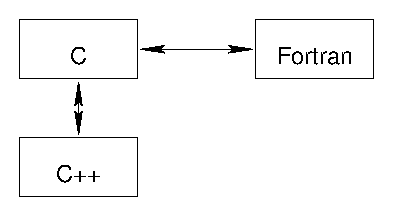
\psfig{file=handle.eps}}
% \begin{verbatim}
%      +-----+         +---------+
%      |  C  | < --- > | Fortran |
%      +-----+         +---------+
%         ^
%         |
%         v
%      +-----+ 
%      | C++ | 
%      +-----+ 
% \end{verbatim}
\caption{Relationship of handle conversion functions.  The C to/from
C++ are part of the C++ binding of MPI.}\label{fig:handle-transfers}
\end{figure}
These are implemented as macros, as permitted by the MPI standard.
The definitions are in \file{mpi.h}.
%% These should normally (i.e., unless
%% \cfgoption{--disable-mpi-macros} is
%% specified to configure) be implemented as macros.  

%% Unresolved question (raised by Barry Smith):  What should happen if
%% the handle is invalid?  Should there even be a check?  Raise the error
%% \mpiconst{MPI_COMM_WORLD} (all errors are on \code{MPI_COMM_WORLD} if
%% no other communicator is specified)?

All handle transfers are handled by casting;
the handle transfer routines are all available as macros, as allowed by
the MPI standard.  The handle transfer routines are:
\mpifunc{MPI_COMM_C2F},
\mpifunc{MPI_COMM_F2C},
\mpifunc{MPI_ERRHANDLER_F2C},
\mpifunc{MPI_ERRHANDLER_C2F},
\mpifunc{MPI_FILE_C2F},
\mpifunc{MPI_FILE_F2C},
\mpifunc{MPI_GROUP_F2C},
\mpifunc{MPI_GROUP_C2F},
\mpifunc{MPI_INFO_F2C},
\mpifunc{MPI_INFO_C2F},
\mpifunc{MPI_OP_F2C},
\mpifunc{MPI_OP_C2F},
\mpifunc{MPI_REQUEST_F2C},
\mpifunc{MPI_REQUEST_C2F},
\mpifunc{MPI_TYPE_C2F},
\mpifunc{MPI_TYPE_F2C},
\mpifunc{MPI_WIN_C2F}, and
\mpifunc{MPI_WIN_F2C}.
These are defined as macros in \file{mpi.h}.  Note that if the handle is
invalid, the error handler associated with \code{MPI_COMM_WORLD} or
\code{MPI_FILE_NULL} (for \code{MPI_File} handles only) should be
invoked.

One weakness of the MPI handle transfer functions is that if there is
an error, such as an invalid handle, there is no easy way to discover
this.  As an extension, we could invoke the error handler on
\code{MPI_COMM_WORLD} (or \code{MPI_FILE_NULL} for file handles) and
set the returned handle to the appropriate NULL handle.  This has not
been implemented.

% \subsubsection{\mpifunc{MPI_COMM_C2F}}
% \subsubsection{\mpifunc{MPI_COMM_F2C}}
% \subsubsection{\mpifunc{MPI_ERRHANDLER_F2C}}
% \subsubsection{\mpifunc{MPI_ERRHANDLER_C2F}}
% \subsubsection{\mpifunc{MPI_FILE_C2F}}
% \subsubsection{\mpifunc{MPI_FILE_F2C}}
% \subsubsection{\mpifunc{MPI_GROUP_F2C}}
% \subsubsection{\mpifunc{MPI_GROUP_C2F}}
% \subsubsection{\mpifunc{MPI_INFO_F2C}}
% \subsubsection{\mpifunc{MPI_INFO_C2F}}
% \subsubsection{\mpifunc{MPI_OP_F2C}}
% \subsubsection{\mpifunc{MPI_OP_C2F}}
% \subsubsection{\mpifunc{MPI_REQUEST_F2C}}
% \subsubsection{\mpifunc{MPI_REQUEST_C2F}}
% \subsubsection{\mpifunc{MPI_TYPE_C2F}}
% \subsubsection{\mpifunc{MPI_TYPE_F2C}}
% \subsubsection{\mpifunc{MPI_WIN_C2F}}
% \subsubsection{\mpifunc{MPI_WIN_F2C}}

\subsubsection{\mpifunc{MPI_STATUS_F2C}}
This needs to recognize the constants \mpiconst{MPI_F_STATUS_IGNORE} and
\mpiconst{MPI_F_STATUSES_IGNORE} (which must be declared in \file{mpi.h}; see
Section 4.12.5 ``Status'' in MPI-2).  

\subsubsection{\mpifunc{MPI_STATUS_C2F}}
Like \mpifunc{MPI_STATUS_F2C}, but must handle the C constants
\mpiconst{MPI_STATUS_IGNORE} and \mpiconst{MPI_STATUSES_IGNORE}.

\subsection{Timers}
\label{sec:timer}
The MPI standard allows \code{MPI_Wtime} and \code{MPI_Wtick} to be
implemented as macros; we should also allow that, at least as an
option.  
The configure option, \cfgoption{--enable-mpi-macros}, causes
\mpifunc{MPI_Wtime} and \mpifunc{MPI_Wtick} to be defined as macros in
\file{mpi.h}. 

Eventually, we should allow for a synchronized timer.  That is, even
if the underlying hardware does not provide a global timer, we should
provide one as an option.  (Earlier versions of the ADI defined a
\mpidfunc{MPID_Gwtime} for this purpose; this has been removed for now
to simplify the ADI.)

One additional feature that should be considered is a way to determine
which timer was chosen.  For example, we could define a predefined
keyval (specific to the MPICH2 implementation) that returned a pointer
to a string that describes the timer.  In general, it might be nice to
have a way to extract configuration (and runtime) choices from an
MPICH2 executable.

%Question: Since we have \mpidfunc{MPID_Gwtime}, should we make that available?

\subsubsection{\mpifunc{MPI_WTICK}}
Call \mpidfunc{MPID_Wtick}.

\subsubsection{\mpifunc{MPI_WTIME}}
Call \mpidfunc{MPID_Wtime}.  If this is the first call to
\mpifunc{MPI_Wtime}, save that value and return zero.  Otherwise, use
\mpidfunc{MPID_Wtime_diff} to convert the time to a double that is
relative to the value of the first call to \mpifunc{MPI_Wtime} and
return that value.
\fixme{We need a test that uses \code{MPI_WTIME_IS_GLOBAL}}
\fixme{We need to describe how a device and/or timer module can set
  \code{MPI_WTIME_IS_GLOBAL}.  We should also provide a runtime option
  to synthesize a global timer.}  

% This requires that \mpifunc{MPI_Init} cause \mpidfunc{MPID_Wtime_init} to be
% called, and that an initial time stamp is stored.

\subsection{Runtime Environment}
\label{sec:runtime-env}
\subsubsection{\mpifunc{MPI_GET_PROCESSOR_NAME}}
Call \mpidfunc{MPID_Get_processor_name}.  

The value of \mpiconst{MPI_MAX_PROCESSOR_NAME} is provided by the
device at configure time, through the Makefile target
\code{echomaxprocname}.  If no value is provided, \code{128} will be used.

\subsubsection{\mpifunc{MPI_GET_VERSION}}
Return the values of \mpiconst{MPI_VERSION} and \mpiconst{MPI_SUBVERSION}. 
Note that this routine can be called anytime, even before \code{MPI_Init} or
after \code{MPI_Finalize}.

\subsection{Profiling}
\label{sec:profile}

\subsubsection{\mpifunc{MPI_PCONTROL}}
This is a simple stub and performs no action other than returning
\mpiconst{MPI_SUCCESS} as the result.  

\subsection{I/O}
\label{sec:io}
MPI I/O is provided by ROMIO.  We plan to update ROMIO to exploit both
MPI-2 functions and to make use of MPID functions (such as the Stream and
Segment modules) when ROMIO is built as part of MPICH2.

There are a few places where we have updated ROMIO to provide better
integration: 
\begin{itemize}
\item I/O requests are integrated with all other MPI requests.  This
  eliminates the need for ROMIO's \code{MPIO_Wait}, \code{MPIO_Test},
  and related multiple completion routines.
\item Error-handlers are consistent with the rest of MPI-2.
  Error reporting follows the rest of MPICH2.
\end{itemize}

% \subsubsection{\mpifunc{MPI_FILE_CALL_ERRHANDLER}}
% \subsubsection{\mpifunc{MPI_FILE_CLOSE}}
% \subsubsection{\mpifunc{MPI_FILE_CREATE_ERRHANDLER}}
% \subsubsection{\mpifunc{MPI_FILE_DELETE}}
% \subsubsection{\mpifunc{MPI_FILE_GET_AMODE}}
% \subsubsection{\mpifunc{MPI_FILE_GET_ATOMICITY}}
% \subsubsection{\mpifunc{MPI_FILE_GET_BYTE_OFFSET}}
% \subsubsection{\mpifunc{MPI_FILE_GET_ERRHANDLER}}
% \subsubsection{\mpifunc{MPI_FILE_GET_GROUP}}
% \subsubsection{\mpifunc{MPI_FILE_GET_INFO}}
% \subsubsection{\mpifunc{MPI_FILE_GET_POSITION}}
% \subsubsection{\mpifunc{MPI_FILE_GET_POSITION_SHARED}}
% \subsubsection{\mpifunc{MPI_FILE_GET_SIZE}}
% \subsubsection{\mpifunc{MPI_FILE_GET_TYPE_EXTENT}}
% \subsubsection{\mpifunc{MPI_FILE_GET_VIEW}}
% \subsubsection{\mpifunc{MPI_FILE_IREAD}}
% \subsubsection{\mpifunc{MPI_FILE_IREAD_AT}}
% \subsubsection{\mpifunc{MPI_FILE_IREAD_SHARED}}
% \subsubsection{\mpifunc{MPI_FILE_IWRITE}}
% \subsubsection{\mpifunc{MPI_FILE_IWRITE_AT}}
% \subsubsection{\mpifunc{MPI_FILE_IWRITE_SHARED}}
% \subsubsection{\mpifunc{MPI_FILE_OPEN}}
% \subsubsection{\mpifunc{MPI_FILE_PREALLOCATE}}
% \subsubsection{\mpifunc{MPI_FILE_READ}}
% \subsubsection{\mpifunc{MPI_FILE_READ_ALL_BEGIN}}
% \subsubsection{\mpifunc{MPI_FILE_READ_AT}}
% \subsubsection{\mpifunc{MPI_FILE_READ_AT_ALL_BEGIN}}
% \subsubsection{\mpifunc{MPI_FILE_READ_ORDERED}}
% \subsubsection{\mpifunc{MPI_FILE_READ_ORDERED_BEGIN}}
% \subsubsection{\mpifunc{MPI_FILE_READ_SHARED}}
% \subsubsection{\mpifunc{MPI_FILE_SEEK}}
% \subsubsection{\mpifunc{MPI_FILE_SEEK_SHARED}}
% \subsubsection{\mpifunc{MPI_FILE_SET_ATOMICITY}}
% \subsubsection{\mpifunc{MPI_FILE_SET_ERRHANDLER}}
% \subsubsection{\mpifunc{MPI_FILE_SET_INFO}}
% \subsubsection{\mpifunc{MPI_FILE_SET_SIZE}}
% \subsubsection{\mpifunc{MPI_FILE_SET_VIEW}}
% \subsubsection{\mpifunc{MPI_FILE_SYNC}}
% \subsubsection{\mpifunc{MPI_FILE_WRITE}}
% \subsubsection{\mpifunc{MPI_FILE_WRITE_ALL_BEGIN}}
% \subsubsection{\mpifunc{MPI_FILE_WRITE_AT}}
% \subsubsection{\mpifunc{MPI_FILE_WRITE_AT_ALL_BEGIN}}
% \subsubsection{\mpifunc{MPI_FILE_WRITE_ORDERED}}
% \subsubsection{\mpifunc{MPI_FILE_WRITE_ORDERED_BEGIN}}
% \subsubsection{\mpifunc{MPI_FILE_WRITE_SHARED}}

% Related constants
% \mpiconst{MPI_MODE_APPEND}
% \mpiconst{MPI_MODE_CREATE}
% \mpiconst{MPI_MODE_DELETE_ON_CLOSE}
% \mpiconst{MPI_MODE_NOCHECK}
% \mpiconst{MPI_MODE_RDONLY}
% \mpiconst{MPI_MODE_SEQUENTIAL}
% \mpiconst{MPI_MODE_UNIQUE_OPEN}
% \mpiconst{MPI_SEEK_CUR}
% \mpiconst{MPI_SEEK_END}
% \mpiconst{MPI_SEEK_SET}
% \mpiconst{MPI_DISPLACEMENT_CURRENT}

\subsection{Utility Routines}
There are a number of utility routines that are discussed in
\file{adi3man.pdf}.

\subsection{Fortran Support}
\label{sec:fortran}
Fortran support has two parts: Fortran 77 and Fortran 90/95.  

There are a few functions unique to Fortran.  They include
\mpifunc{MPI_SIZEOF} and \mpifunc{MPI_TYPE_CREATE_F90_COMPLEX}, 
\mpifunc{MPI_TYPE_CREATE_F90_REAL}, and 
\mpifunc{MPI_TYPE_CREATE_F90_INTEGER}.  Note that the \code{TYPE_CREATE}
routines create types that must return the corresponding combiner names when
\mpifunc{MPI_TYPE_GET_ENVELOPE} is called and that these must be
``predefined'' types; that is, they cannot be freed.

\subsubsection{\mpifunc{MPI_SIZEOF}}
This must be implemented in an MPI module.  The implementation looks something
like this:
\begin{verbatim}
       MODULE MPI2__REAL_s
       PRIVATE
       PUBLIC :: MPI_SIZEOF
       INTERFACE MPI_SIZEOF
           MODULE PROCEDURE MPI_SIZEOF_T
       END INTERFACE
       CONTAINS
       SUBROUTINE MPI_SIZEOF_T( X, SIZE, IERROR )
       REAL X
       INTEGER SIZE, IERROR
       IERROR = 0
       SIZE   = 4
       END SUBROUTINE MPI_SIZEOF_T       
       END MODULE
\end{verbatim}
Each Fortran type (including each type passed as an array, and for
each number of dimensions of the array) requires a similar
definition.  The actual size (four in the example above) must be determined by
configure or provided by the user.
These can be created automatically in a way similar to the current
Fortran 90 interface.

This has been added to the Fortran 90 support in MPICH-1, although the
handling of type sizes should be better; sizes are set expecting the
\code{*n} format.  If another format is used, such as plain type
names, the current code chooses the common (but not universal) defaults.

\subsubsection{\mpifunc{MPI_TYPE_CREATE_F90_INTEGER}}
This searches through a global list (pointed at by
\mpidconst{MPID_F90_Predefined_types_head}) to see if the requested type has
already been allocated.  If so, it returns that type.  
If not, it must allocate a new predefined type, initialize all of the fields,
including the envelope type of \mpiconst{MPI_COMBINER_F90_INTEGER} and the
\code{digits} field, and returns that new type.
In a multithreaded case, this list must be updated in a thread-safe manner
(e.g., by locking the list).

The implementation will use a small array instead of a list?  If the
user asks for too many distinct types, we can return an
\mpiconst{MPI_ERR_OTHER} class indicating the problem.  Should this
cause any real and correct programs problems, we can look into using a
list or other dynamically-sized structure.

Also, like many other modules, this module uses lazy initialization
and a finalize callback.

%% Question:
%% Should there be a separate routine to initialize this array and to free the
%% datatypes that are created during \mpifunc{MPI_Finalize}?  (I think so,
%% particularly when trying to streamline codes to requiring only single-language
%% support.)  What are the names of the routines?  Is there a common file that
%% contains \mpidconst{MPID_F90_Predefined_types_head} as well as the routines to
%% allocate and free these predefined types?  See also the finalize
%% callbacks in \mpifunc{MPI_Finalize}.  Answer: yes.

\subsubsection{\mpifunc{MPI_TYPE_CREATE_F90_REAL}}
See \mpifunc{MPI_TYPE_CREATE_F90_INTEGER}.

\subsubsection{\mpifunc{MPI_TYPE_CREATE_F90_COMPLEX}}
See \mpifunc{MPI_TYPE_CREATE_F90_INTEGER}.

\subsubsection{Fortran Wrappers}
One added complexity of the Fortran wrappers is handling the possibility that
the types \code{MPI_Fint} and \code{int} have different sizes.
\fixme{This is not yet handled}
When the
Fortran codes simply call the C codes, this results in copying array arguments
to a temporary array, calling the C code, and freeing the array.  Allocation
and deallocation of small arrays can be avoided by using local arrays (to be
thread-safe).  However, it is best to avoid these copies and
allocation/deallocations whenever possible.  Thus, we
need a CPP value that indicates whether \code{MPI_Fint} and \code{int} are the
same size.  This CPP name is \mpifunc{HAVE_FINT_IS_INT} and is
determined by the \code{configure} in \file{src/binding/f77}.

%% In addition, the MPICH Fortran wrapper code is intended for use with MPE and
%% other MPI implementations, and makes no assumptions about the structure of
%% MPI opaque objects, necessitating a transfer of values for each array-value
%% argument.  I'd like to avoid this as well.  Can we ignore the other MPI's, or
%% use special routines as part of the MPE support?  Alternately, should we
%% define \code{MPICH_REQUEST_C_IS_F77} etc.?

\subsubsection{Fortran Datatypes}
There are several special Fortran datatypes that do not have simple C
counterparts.  These are
\begin{description}
\item[\code{LOGICAL}.]Roughly like the \code{bool} type in C++, the choice of
  value for \code{.true.} and \code{.false.} is left to the implementation.
  In MPICH, we use \code{MPIR_F_TRUE} and \code{MPIR_F_FALSE} as values.
\item[\code{COMPLEX} and \code{COMPLEX*16}.]These are universally implemented
  as a pair of \code{REAL}s or \code{DOUBLE PRECISION} values.
\end{description}

\subsection{C++ Support}
\label{sec:c++}

Like the Fortran 77 bindings, the C++ bindings are generated
automatically, using the script \file{buildiface} and the
\file{mpi.h.in} file.  This implementation does not create the C++
profiling interface; the MPI standard allows an implementation to
provide only the C (and Fortran) profiling interface.  

\subsection{C\# Support}
\label{sec:csharp}

MPICH2 will provide an experimental interface for C\# programmers.  As
there is no standard definition for an MPI binding to C\#, this
interface will be based on the C++ binding, though possible with a
different approach to the profiling interface.

%% I'd like to consider adding more native C++ support.  While the
%% Indiana (formerly Notre
%% Dame) C++ code is valuable and helpful, there are some difficulties:
%% \begin{enumerate}
%% \item Supports only MPI-1.

%% \item Their configure is based too much on particular systems rather than on
%% capabilities. 

%% \item Because it is a separate package, the build process is awkward.

%% \item Testing is separate from the MPICH testing, causing inadequate
%% testing of the MPICH/C++ combination.

%% \item Layering makes some things difficult; it can be awkward because
%% some data structures must be duplicated since MPI itself leaves them
%% opaque.  For example, the C++ \code{Comm} could contain a pointer to the
%% \mpidconst{MPID_Comm}, rather than the opaque object \code{MPI_Comm}.

%% \item Does not pass our (sometimes stricter) coding standards (of course, our
%%   code doesn't pass theirs either).

%% \item Their code must deal with a wide variety of partial C++
%% implementations.  Perhaps by 2004, there will be fewer bugs in C++ compilers.
%% \end{enumerate}

%% Question: Is there a way to automate the generation of most of these routines?
%% Or should we just write them out?  Answer: They are different enough that we
%% need to write them out.

%% I've started the implementation of this.  See \file{mpich/src/cxx} in the
%% MPICH-1 implementation.

%% This section should contain some of the discussion from \file{adi3man.tex} on data
%% structures and constants, particularly the handle allocator, and the reference
%% count routines.  

%\let\SaveBibliography=\thebibliography
%\def\thebibliography#1{\SaveBibliography{#1}\addcontentsline{toc}{section}{References}}

% \section{Appendix}
% This section contain \emph{all} of the MPI functions and terms.  These
% will be moved into the body of this document; an index will then
% replace this appendix.  Until then, this section serves as a place to
% cache these items.

%\subsection{Constants}
%(I need to get the union of MPI-1 and MPI-2 constants)

% \subsection{Typedefs}
% \code{MPI_Aint}\\
% \code{MPI_Comm_copy_attr_function}\\
% \code{MPI_Comm_errhandler_fn}\\
% \code{MPI_Datarep_conversion_function}\\
% \code{MPI_Datarep_extent_function}\\
% \code{MPI_File_errhandler_fn}\\
% \code{MPI_Grequest_cancel_function}\\
% \code{MPI_Type_copy_attr_function}\\
% \code{MPI_Win_copy_attr_function}\\
% \code{MPI_Win_errhandler_fn}\\

% %%
% %% Temporary
% \clearpage
% Accessing this document.  Use one of:
% \begin{enumerate}
% \item \code{cvs -d /home/MPI/cvsMaster checkout mpich2-coding}
% \item \code{cvs -d /home/MPI/cvsMaster checkout mpich2all; cd doc/mpich2}
% \item \code{cd mpich2/doc ; cvs -q update -d}, only if you have previously checked
%   \code{mpich2} out with \code{mpich2all} instead of \code{mpich2}.
% \end{enumerate}
% %% End of Temporary

\section{ToDo List}
\label{sec:todo}
This section contains a ToDo list for this document; that is, the outstanding
issues and questions.  The process for resolving each of these is to have each
item choosen by one person who is responsible for writing the text (the
section author) and one
other person who is the ``immediate reviewer.''  The section author is
responsible for 
organizing and leading any discussion necessary to complete the text.
Anyone may read and comment on the document at any time, but should check with
the section author first to make sure that the document is up-to-date.
Once a section is written, it should be read by everyone and we should
``vote'' on the section.  Once a section is ``passed,'' the section author
should update the ADI-3 document to match the section.  This may involve
changing, adding, and/or deleting routines from the ADI-3 document.  Once that
step is completed, the routines in the section can be written.  The section
author is \emph{not} responsible for implementing the routines in the
section (though they can be; the point is that authoring a section is separate
from implementing a section).  

Many of these sections can be implemented independently, once the
infrastructure list is settled. 
\begin{enumerate}
%\item Infrastructure
%
%  These are necessary before any coding can commence.
%  \begin{enumerate}
%    \item Directory structure
%    \item MPI routine source code template, including error checks
%    \item Partial definitions for key structures, such as communicators and
%      datatypes, and macros for thread-safe operations
%    \item Coding standards (documentation, style, associated tests)
%    \item Integral profiling and data collection.  Definition of macros for
%      collecting timing data and for generating slog records.
%  \end{enumerate}
%  In addition, the error reporting routines and guidelines to error handling
%  are needed before much coding is done.

\item MPI Major Sections

  Each of these sections should consider
  \begin{enumerate}
    \item Thread safety,
    \item Error handling and reporting,
%    \item Core ADI for 3rd parties (non-multimethod),
    \item Core method ADI for 3rd parties (as part of our multimethod device),
      and 
    \item Performance in MPI communication (whether point-to-point,
      collective, or RMA).
    \end{enumerate}
    In addition, scalability to 10,000 processes is required and scalability
    beyond that to 1,000,000 processes should be considered.  However, if
    scalability to a million processes complicates the design or the code, we
    should design for fewer processes and document the reasons in the
    Rationale (Section~\ref{sec:rationale}).

%%     The highest-priority items are: Point-to-point, collective, RMA, and
%%     dynamic processes, along with the communication agent.  Of course, these
%%     will require some specification of datatypes, communicators, groups, etc.,
%%     but they will also drive the details of those objects (e.g., datatypes
%%     must be defined to support the operations needed for communication).

% Rob - point to point
% Bill - collective
% Rusty - dynamic process
% Rob/Brian - communication agent

  Other items include:

  \begin{enumerate}
%  \item Attributes. 
  \item Info.
\paragraph{Defining New Info Keys.}
The MPI Forum has not resolved an ambiguity in the definition of
info.  While it was clear during many of the discussions that the
expectation was that \code{MPI_Info}\index{MPI_Info} could be used by
layered implementations of parts of MPI, particularly the I/O part,
IBM did not interpret the standard this way and their interpretation
is both consistent with the standard and offers a feature not
otherwise available (specifically, the ability to determine what info
keys are recognized by the implementation).  However, we have chosen to follow
the spirit of the MPI Forum and allow users to create their own keys.


%  \item Datatypes.
%  \item Groups.
%  \item Point-to-point.  
%    \begin{enumerate}
%%     \item Make the scenario (Section~\ref{sec:pt-2-pt-scenarios})
%%       consistent with the description of the individual routines and with
%%       the most current discussions of the active queue implementation,
%%       including the support of collective communication.
%    \item Define the communicator data structure, including the handling
%      of processes that are not part of the original
%      \mpiconst{MPI_COMM_WORLD}.
%    \item Address the issues of the multiple completion routines (e.g.,
%      \mpifunc{MPI_Waitsome}). 
%    \end{enumerate}
  \item Communication agent. 
    This ensures the progress of MPI communication including passive RMA
    access.  As such, it is closely connected to the point-to-point and RMA
    sections.  
  \item Collective.  
    \begin{enumerate}
%%     \item \mpifunc{MPI_Bcast}, \mpifunc{MPI_Scatter}, and \mpifunc{MPI_Reduce}
%%       with ``stream'' operations.
%%     \item Plan for developing algorithms for the other collective routines.
    \item Design to allow implementors to replace any collective routine with
      a device-specific version.  See the description in
      \file{doc/develop/collop.tex}.
    \end{enumerate}
%%   \item Communicators.
%%     \begin{enumerate}
%%     \item Basic routines for communicator construction.  Coordinate intercomm
%%       creation with the dynamic process routines (\mpifunc{MPI_Comm_spawn},
%%       \mpifunc{MPI_Comm_connect}, \mpifunc{MPI_Comm_attach}, and
%%       \mpifunc{MPI_Join}).  
%%     \end{enumerate}
%%   \item Topology.
%%   \item RMA.  Everything (including scenarios illustrating BSP-style defered
%%     updates).  
%%   \begin{enumerate}
%%     \item Scenarios
%%   \end{enumerate}
%%   \item Starting and Ending MPI (e.g., init, finalize, and abort).
%%   \item Dynamic processes.
%%   \item Name service.
%%   \item User-defined requests (also needed for ROMIO I/O).
%%   \item Error handlers. (These are the MPI error handlers, not the error
%%     reporting routines.)
%%   \item Handle Transfers (e.g., \code{MPI_Request_c2f})
%%   \item Timers.
%%   \item I/O.  For the most part, we will take ROMIO without any changes for
%%     now.  However, there are a few things to handle:
%%     \begin{enumerate}
%%     \item Replace ROMIO's \code{MPIO_Request} and \code{MPIO_Wait} etc. with
%%       regular \code{MPI_Request}s (possibly using the generalized requests).
%%     \item Update error reporting with new routines
%%     \item Check on datatype handling
%%     \item Update \file{configure.in}
%%     \end{enumerate}
%%   \item Runtime Environment.  (Processor name and MPI version.)
%%   \item Profiling.
%%   \item MPI command environment (\code{mpiexec}, \code{mpicc}, etc.)
  \end{enumerate}
\item Source code, portability, and framework.
  These are miscellaneous (though important) items that need to be completed
  before much coding is done.  Most of the issues mentioned in
  previous versions have been handled; only the outstanding issues are
  listed here.

  \begin{enumerate}
  \item Error reporting routines, particularly the handling of
    instance-specific messages and internationalization.
  \item mpich2 bug list.  In particular, how will provide an open bug list?
%%   \item Runtime parameter access (e.g., socket buffer sizes from an
%%     environment variable or \file{.mpichrc} file).
%%   \item Configure and automake, particularly a style-sheet on modifying the
%%     autoconf and automake input files.  See \file{maint/sampleconf.in}.
%%   \item Cross compilation and compilation environment (using different
%%     compilers from the ones MPICH is built with)
%%   \item Fortran
%%   \item C++
%%   \item Testing.  Needs new test harness; intelligent sampling of the possible
%%     combinations; archiving of results (including performance tests).  The
%%     tests must work with any MPI, not just MPICH (just like the current test
%%     suite).  Separate tests for MPICH-specific features should be provided in
%%     a separate suite of tests.
  \end{enumerate}
\end{enumerate}

% \section{Development Plan}
% \label{sec:development}
% This section proposes a development and implementation plan.  The
% emphasis here is on independent subprojects, allowing development to
% proceed without waiting for all of the pieces to be in place.

% \begin{enumerate}
% \item ADI Implementation
%     \begin{enumerate}
%     \item Design Development
%         \begin{enumerate}
%         \item Design and implement a subset of general datatype pack/unpack
%         \item Design and implement a subset (e.g., Allreduce, Bcast, and
%           Alltoall) of collective operations using the Stream and Segment MPID
%           functions.
%         \item Test improved collectives for performance and functionality
%         \item Similar design/implement/test for RMA and Dynamic; details yet
%           to be determined.
%         \end{enumerate}
%     \item Multi-method ADI for shared memory, VIA, and TCP/UDP
%         \begin{enumerate}
%         \item Design and implement general datatype point-to-point
%         \item Design and implement general datatype collective
%         (layered on ADI segment and stream interfaces)
%         \item Design and implement RMA
%         \item Design and implement Dynamic and connect with BNR
%         \end{enumerate}
%     \item ADI on \code{MPID_CORE}
%         \begin{enumerate}
%         \item Implement all ADI-3 modules on top of the core.  Refine
%         the design of the core during this process.   
%         \end{enumerate}
%     \item Implement common ADI services.  These are modules that are
%     needed by other ADI modules that do not (directly) involve
%     interprocess communication but will be common for most ADI
%     implementations, including both the core and the multi-method
%     implementation. 
%         \begin{enumerate}
%         \item Error handling
%         \item Attributes
%         \item Info
%         \item Runtime parameters
%         \item Topology
%         \item Datatype
%         \item Group
%         \item Timer
%         \item Utility
%         \end{enumerate}
%     \end{enumerate}
% \item MPICH Implementation on ADI
%     \begin{enumerate}
%     \item For each MPI routine, write the ``top'': structured comment,
%     routine header and error checking.
%     \item Implement the action of each MPI routine in terms of the
%     full ADI-3 design.
%     \end{enumerate}
% \item Test Suite
%     \begin{enumerate}
%     \item Design standard test harness: test communicators, datatypes,
%     operation mixtures, run script, and result checking.
%     \end{enumerate}
% \item Deployment
%     \begin{enumerate}
%     \item Implement new configure.  Design database for both configure
%     macros and for data (such as compiler options and names) that
%     configure cannot determine.
%     \item Shared library support.
%     \end{enumerate}
% \end{enumerate}

%
% Eventually include table or a project as Postscript from project.
%
\part{Appendices}

\appendix

\section{Error Codes}
\label{sec:error-codes}

%
% This file contains the error classes/codes section so that it can be
% separately printed.
\subsubsection{Error Classes and Codes}
The MPI standard defines a number of error classes and permits an
implementation to make use of additional error codes, with the proviso that
any error code belong to some error class (though this does include the
\mpiconst{MPI_ERR_OTHER} class).  
The specification of MPI error classes is rather uneven.  There are separate
classes for most of the arguments to the point-to-point communication
functions and for many of the I/O errors.  Other routines have to make due
with \mpiconst{MPI_ERR_ARG} or \mpiconst{MPI_ERR_OTHER}.

In addition, many of the errors have common subcases.  For example, most of
the errors that refer to an MPI opaque handle can indicate either a null or a
non-null but invalid handle.   To handle all of these cases, we predefine an
extended set of error codes.  Only the error classes are defined in
\file{mpi.h}; the others are defined in \file{mpiimpl.h} (Question: is this
the correct place, or should there be a separate file?).  The additional error
codes all have the form of \code{MPIi_ERR_<class>_<subclass>}.  For example,
the code for a null communicator is \mpiconst{MPIi_ERR_COMM_NULL}.

Comment [BRT]: I find that MPIi_ is painful to type.  Is there a
reason the second `i' is lowercase?

Many of these descriptions list the optional arguments.  These can be provided
(in the order and with the types specified) to the call that creates an error
code (see \mpidfunc{MPID_Err_create_code}). 

\begin{description}
\item[\mpiconst{MPI_ERR_BUFFER}]Invalid buffer pointer
    \begin{description}
    \item[\mpidconst{MPIi_ERR_BUFFER_NULL}]Null buffer pointer
    \item[\mpidconst{MPIi_ERR_BUFFER_NOSPACE}]Insufficient space in Bsend
      buffer (optional args: requested and avaliable length (int))
    \item[\mpidconst{MPIi_ERR_BUFFER_ALIAS}]Buffers must not be aliased
      (optional args: names of two arguments (string))
    \item[\mpidconst{MPIi_ERR_BUFFER_SIZE}]Invalid buffer size (optional arg:
      size (int))
    \item[\mpidconst{MPIi_ERR_BUFFER_BSEND_EXISTS}]Buffer already attached with
      \mpifunc{MPI_BUFFER_ATTACH}. 
    \item[\mpidconst{MPIi_ERR_BUFFER_BSEND_SMALL}]Buffer size is smaller than
      \mpiconst{MPI_BSEND_OVERHEAD} (optional argument: size, value of
      \code{MPI_BSEND_OVERHEAD} (int)) 
    \item[\mpidconst{MPIi_ERR_BUFFER_BSEND_NONE}]No buffer to detach.
    \end{description}
\item[\mpiconst{MPI_ERR_COUNT}]Invalid count (optional argument value (int))
    \begin{description}
    \item[\mpidconst{MPIi_ERR_COUNT_ARRAY}]Invalid count in count array
      (optional arguments: index and value (int))
    \end{description}
\item[\mpiconst{MPI_ERR_TYPE}]Invalid datatype
    \begin{description}
    \item[\mpidconst{MPIi_ERR_TYPE_NULL}]Null datatype
    \item[\mpidconst{MPIi_ERR_TYPE_ARRAY_NULL}]Null datatype in array of
      datatypes (optional arguments: name of argument (string) and index (int))
    \item[\mpidconst{MPIi_ERR_TYPE_NOT_COMMITTED}]Datatype has not been
      committed 
    \item[\mpidconst{MPIi_ERR_TYPE_FREE_PERM}]Cannot free permanent data type
      (optional argument: name (string))
    \item[\mpidconst{MPIi_ERR_TYPE_PERM_CONTENTS]}]Cannot get contents of a
      permanent or basic data type (optional argument: name (string))
    \item[\mpidconst{MPIi_ERR_TYPE_NAME}]Cannot set name in data type
    \item[\mpidconst{MPIi_ERR_TYPE_NOMATCH}]Type signatures do not
    match in communication (see \cite{gro:mpi-datatypes:pvmmpi00})
    \item[\mpidconst{MPIi_ERR_TYPE_WRONG_COMM}]Pack buffer not packed
    for this communicator.  
\cite{})
    \end{description}
\item[\mpiconst{MPI_ERR_TAG}]Invalid tag (optional argument: value (int) )
%    \begin{description}
%    \item[\mpidconst{MPIi_ERR_}]
%    \end{description}
\item[\mpiconst{MPI_ERR_COMM}]Invalid communicator
    \begin{description}
    \item[\mpidconst{MPIi_ERR_COMM_NULL}]Null communicator
    \item[\mpidconst{MPIi_ERR_COMM_INTER}]Intercommunicator is not allowed
    \item[\mpidconst{MPIi_ERR_COMM_INTRA}]Intracommunicator is not allowed
    \item[\mpidconst{MPIi_ERR_COMM_NAME}]Cannot set name in communicator
    \item[\mpidconst{MPIi_ERR_COMM_PEER}]Peer communicator is not valid
    \item[\mpidconst{MPIi_ERR_COMM_LOCAL_NULL}]Local communicator must not be
      \mpiconst{MPI_COMM_NULL}
    \end{description}
    Note that while C++ defines separate Cartesian and Graph
    communicators, errors involving improper choice of those is under
    \mpiconst{MPI_ERR_TOPOLOGY}. 
\item[\mpiconst{MPI_ERR_RANK}]Invalid rank (optional argument: value (int))
    \begin{description}
    \item[\mpidconst{MPIi_ERR_RANK_ARRAY}]Invalid rank in rank array (optional
      arguments: index, value, size-1 (int))
    \item[\mpidconst{MPIi_ERR_RANK_DUP}]Duplicate ranks in rank array
      (optional arguments: index, value, other index (int))
    \item[\mpidconst{MPIi_ERR_RANK_LOCAL}]Error specifying local_leader
      (optional arguments: value, size-1 (int))
    \item[\mpidconst{MPIi_ERR_RANK_REMOTE}]Error specifying remote_leader
      (optional arguments: value, size-1 (int))
    \end{description}
\item[\mpiconst{MPI_ERR_ROOT}]Invalid root (optional arg: value (int))
    \begin{description}
    \item[\mpidconst{MPIi_ERR_ROOT_LARGE}]Root is too large (optional
      arguments: value and size-1 (int))
    \end{description}
\item[\mpiconst{MPI_ERR_GROUP}]Invalid group
    \begin{description}
    \item[\mpidconst{MPIi_ERR_GROUP_NULL}]Null group
    \end{description}
\item[\mpiconst{MPI_ERR_OP}]Invalid \mpiconst{MPI_Op}
    \begin{description}
    \item[\mpidconst{MPIi_ERR_OP_NULL}]Null \mpiconst{MPI_Op}
    \item[\mpidconst{MPIi_ERR_OP_UNDEFINED}]\mpiconst{MPI_Op} operation not
      defined for 
      this datatype (optional argument: name of datatype (string))
    \item[\mpidconst{MPIi_ERR_OP_FREE_PERM}]Cannot free permanent
      \mpiconst{MPI_Op} 
    \end{description}
\item[\mpiconst{MPI_ERR_TOPOLOGY}]Invalid topology
    \begin{description}
    \item[\mpidconst{MPIi_ERR_TOPOLOGY_SIZE}]Topology size is greater than
      communicator size (optional arguments: topology size and communicator
      size (int))
    \item[\mpidconst{MPIi_ERR_TOPOLOGY_GRAPH_ARRAY_SIZE}]Specified edge $<$ 0
      or $>$ nnodes (optional arguments: index, value, nnodes (int))
    \end{description}
\item[\mpiconst{MPI_ERR_DIMS}]Invalid dimension argument (optional arg: value (int))
    \begin{description}
    \item[\mpidconst{MPIi_ERR_DIMS_ARRAY}]Invalid dimension argument in array
      (optional arguments: index, value (int))
    \item[\mpidconst{MPIi_ERR_DIMS_MANY}]Number of dimensions is too large
      (optional arguments: value, maxvalue (int))
    \item[\mpidconst{MPIi_ERR_DIMS_TENSOR_SIZE}]Tensor product size does not
      match nnodes (optional arguments: tensor product size and nnodes (int))
    \item[\mpidconst{MPIi_ERR_DIMS_PARTITION}]Can not partition nodes as
      requested 
    \end{description}
\item[\mpiconst{MPI_ERR_ARG}]Invalid argument (optional arg: name (string))
    \begin{description}
    \item[\mpidconst{MPIi_ERR_ARG_ERRCODE}]Invalid error code (optional arg:
      value (int))
    \item[\mpidconst{MPIi_ERR_ARG_NULL}]Invalid null parameter (optional arg:
      name of argument (string))
    \item[\mpidconst{MPIi_ERR_ARG_F77_ADDRESS}]Address of location given to
      \mpifunc{MPI_ADDRESS} does not fix in a Fortran integer (optional
      argument: address (long int))
    \item[\mpidconst{MPIi_ERR_ARG_ERRHANDLER}]Invalid errhandler
    \item[\mpidconst{MPIi_ERR_ARG_ERRHANDLER_NULL}]Null errhandler
    \item[\mpidconst{MPIi_ERR_ARG_ERRHANDLER_FREE_PERM}]Cannot free permanent
      error handler (optional argument: name (string))
    \item[\mpidconst{MPIi_ERR_ARG_STATUS_IGNORE}]Invalid use of
      \mpiconst{MPI_STATUS_IGNORE} or \mpiconst{MPI_STATUSES_IGNORE}
    \item[\mpidconst{MPIi_ERR_ARG_STRIDE}]Range does not terminate (optional
      arguments: start, end, stride (int))
    \item[\mpidconst{MPIi_ERR_ARG_STRIDE_ZERO}]Zero stride is incorrect
    \item[\mpidconst{MPIi_ERR_ARG_ARRAY_VAL}]Invalid value in array (optional
      arguments: name of variable (string), index (int), value (int))
    \item[\mpidconst{MPIi_ERR_ARG_NAMED}]Invalid argument (optional arguments:
      name (string), value (int))
    \item[\mpidconst{MPIi_ERR_ARG_NEGATIVE}]Invalid argument; must be
      nonnegative (optional arguments: name (string), value (int))
    \item[\mpidconst{MPIi_ERR_ARG_ARRAY_VAL_NEG}]Negative value in array
      (optional arguments: name of variable (string), index (int), value
      (int)) 
    \item[\mpidconst{MPIi_ERR_ARG_DARRAY_DIST_NONE}]For
      \mpiconst{MPI_DISTRIBUTE_NONE}, the number of processes in that
      dimension of the grid must be 1 (optional arguments: index of
      array_of_psizes, value (int))
    \item[\mpidconst{MPIi_ERR_ARG_DARRAY_DIST_UNKNOWN}]Unknown distribution
      type 
    \item[\mpidconst{MPIi_ERR_ARG_DARRAY_INVALID_BLOCK}]Value of m must be
      positive for block(m) distribution (optional argument: value of m (int))
    \item[\mpidconst{MPIi_ERR_ARG_DARRAY_INVALID_BLOCK2}]\code{m * nprocs} is
      $<$ \code{array_size} and is not valid for block(m) distribution
      (optional arguments: \code{m*nprocs}, \code{array_size} (int))
    \item[\mpidconst{MPIi_ERR_ARG_DARRAY_INVALID_CYCLIC}]Value of m must be
      positive for a cyclic(m) distribution (optional argument: m (int))
    \item[\mpidconst{MPIi_ERR_ARG_POSITION_NEG}]Value of position must be
      nonnegative (optional argument: value (int))
    \item[\mpidconst{MPIi_ERR_ARG_INFO_NKEY}]n is invalid (optional arguments:
      n, number of keys in info (int))
    \end{description}
\item[\mpiconst{MPI_ERR_UNKNOWN}]Unknown error.  Note that this should
  \emph{never} be used.
%    \begin{description}
%    \item[\mpidconst{MPIi_ERR_}]
%    \end{description}
\item[\mpiconst{MPI_ERR_TRUNCATE}]Message truncated (optional arguments: bytes
  received and buffer size (int))
%    \begin{description}
%    \item[\mpidconst{MPIi_ERR_}]
%    \end{description}
\item[\mpiconst{MPI_ERR_OTHER}]Other MPI error
    \begin{description}
    \item[\mpidconst{MPIi_ERR_OTHER_RESOURCE}]System resource limit exceeded
      (optional argument: name of resource (string))
    \item[\mpidconst{MPIi_ERR_OTHER_RSEND}]Ready send had no matching receive
      (optional arguments: source, destination, tag (int))
    \item[\mpidconst{MPIi_ERR_OTHER_INIT_TWICE}]Cannot call \mpifunc{MPI_INIT}
      or \mpifunc{MPI_INIT_THREAD} more than once
    \item[\mpidconst{MPIi_ERR_OTHER_INIT_BEFORE}]\mpifunc{MPI_Init} must be
      called first (optional argument: name of calling routine (string))
    \item[\mpidconst{MPIi_ERR_OTHER_STARTUP}]Error on startup, such as a
      mismatch between \code{mpiexec} and the MPI libraries (optional
      argument: text with detailed reason (string))
    \item[\mpidconst{MPIi_ERR_OTHER_NOMEM}]Out of memory (optional arguments:
      requested and available (int))
    \item[\mpidconst{MPIi_ERR_OTHER_ATTR_COPY}]User defined attribute copy
      routine returned a non-zero return code (optional argument: return code
      (int)) 
    \end{description}
\item[\mpiconst{MPI_ERR_INTERN}]Internal MPI error!  (optional argument:
  detailed text (string))
These provide English-only strings because they are for internal errors and
should never be seen by users.
%    \begin{description}
%    \item[\mpidconst{MPIi_ERR_INTERN}]
%    \end{description}
\item[\mpiconst{MPI_ERR_IN_STATUS}]See the \mpiconst{MPI_ERROR} field in
  \mpiconst{MPI_Status} for the error code
%    \begin{description}
%    \item[\mpidconst{MPIi_ERR_}]
%    \end{description}
\item[\mpiconst{MPI_ERR_PENDING}]Pending request (no error)
%    \begin{description}
%    \item[\mpidconst{MPIi_ERR_}]
%    \end{description}
\item[\mpiconst{MPI_ERR_REQUEST}]Invalid \mpiconst{MPI_Request}
    \begin{description}
    \item[\mpidconst{MPIi_ERR_REQUEST_NULL}]Null \mpiconst{MPI_Request}
    \item[\mpidconst{MPIi_ERR_REQUEST_NOT_PERSISTENT}]Request is not
      persistent in \mpifunc{MPI_Start} or \mpifunc{MPI_Startall}.
    \end{description}
\item[\mpiconst{MPI_ERR_ACCESS}]Access denied to file (optional arg: name (string)
%    \begin{description}
%    \item[\mpidconst{MPIi_ERR_}]
%    \end{description}
\item[\mpiconst{MPI_ERR_AMODE}]Invalid amode value in \mpifunc{MPI_File_open}
  (optional argument: amode (int))
    \begin{description}
    \item[\mpidconst{MPIi_ERR_AMODE_ONLY_ONE}]Exactly one of
      \mpiconst{MPI_MODE_RDONLY}, \mpiconst{MPI_MODE_WRONLY}, or
      \mpiconst{MPI_MODE_RDWR} must be specified
    \item[\mpidconst{MPIi_ERR_AMODE_RDONLY}]Cannot use
      \mpiconst{MPI_MODE_CREATE} or \mpiconst{MPI_MODE_EXCL} with
      \mpiconst{MPI_MODE_RDONLY} 
    \item[\mpidconst{MPIi_ERR_AMODE_SEQ}]Cannot specify
      \mpiconst{MPI_MODE_SEQUENTIAL} with \code{MPI_MODE_RDWR}
    \end{description}
\item[\mpiconst{MPI_ERR_BAD_FILE}]Invalid file name (optional arg: name
  (string)) 
    \begin{description}
    \item[\mpidconst{MPIi_ERR_BAD_FILE_LONG}]Pathname too long (optional
      arguments: name, length, and maximum length (string, int, int))
    \item[\mpidconst{MPIi_ERR_BAD_FILE_DIR}]Invalid or missing directory
      (optional argument: name (string))
    \end{description}
\item[\mpiconst{MPI_ERR_CONVERSION}]An error occurred in a user-defined data
  conversion function
%    \begin{description}
%    \item[\mpidconst{MPIi_ERR_}]
%    \end{description}
\item[\mpiconst{MPI_ERR_DUP_DATAREP}]The requested datarep name has already
  been specified to \mpifunc{MPI_REGISTER_DATAREP} (optional arg: name
  (string))
%    \begin{description}
%    \item[\mpidconst{MPIi_ERR_}]
%    \end{description}
\item[\mpiconst{MPI_ERR_FILE_EXISTS}]File exists (optional arg: name (string))
%    \begin{description}
%    \item[\mpidconst{MPIi_ERR_}]
%    \end{description}
\item[\mpiconst{MPI_ERR_FILE_IN_USE}]File in use by some process (optional
  arg: name (string))
%    \begin{description}
%    \item[\mpidconst{MPIi_ERR_}]
%    \end{description}
\item[\mpiconst{MPI_ERR_FILE}]Invalid \mpiconst{MPI_File}
    \begin{description}
    \item[\mpidconst{MPIi_ERR_FILE_NULL}]Null \mpiconst{MPI_File}
    \end{description}
\item[\mpiconst{MPI_ERR_INFO}]Invalid \mpiconst{MPI_Info}
    \begin{description}
    \item[\mpidconst{MPIi_ERR_INFO_NULL}]Null \mpiconst{MPI_Info}
    \end{description}
\item[\mpiconst{MPI_ERR_INFO_KEY}]Invalid key for \mpiconst{MPI_Info}
    \begin{description}
    \item[\mpidconst{MPIi_ERR_INFO_KEY_NULL}]Null key
    \item[\mpidconst{MPIi_ERR_INFO_KEY_LENGTH}]Key is too long (optional
      arguments: name, length, maxlength (string, int, int )
    \item[\mpidconst{MPIi_ERR_INFO_KEY_EMPTY}]Empty or blank key
    \end{description}
\item[\mpiconst{MPI_ERR_INFO_VALUE}]Invalid \mpiconst{MPI_Info} value
    \begin{description}
    \item[\mpidconst{MPIi_ERR_INFO_VALUE_NULL}]Null value
    \item[\mpidconst{MPIi_ERR_INFO_VALUE_LENGTH}]Value is too long (optional
      arguments: name, length, maxlength (string, int, int)
    \end{description}
\item[\mpiconst{MPI_ERR_INFO_NOKEY}]\mpiconst{MPI_Info} key is not defined
  (optional argument: keyname (string))
%    \begin{description}
%    \item[\mpidconst{MPIi_ERR_}]
%    \end{description}
\item[\mpiconst{MPI_ERR_IO}]Other I/O error (optional argument: text (string))
    \begin{description}
    \item[\mpidconst{MPIi_ERR_IO_ETYPE_FRACTIONAL}]Only an integral number of
      etypes can be accessed
    \item[\mpidconst{MPIi_ERR_IO_NO_FSTYPE}]Cannot determine filesystem type
      (optional argument: name of file (string))
    \item[\mpidconst{MPIi_ERR_IO_UNAVAILABLE_FSTYPE}]Specified filesystem is
      not available (optional argument: name of filesystem (string))
    \item[\mpidconst{MPIi_ERR_IO_MULTIPLE_SPLIT_COLL}]Only one active split
      collective I/O operation is allowed per file handle
    \item[\mpidconst{MPIi_ERR_IO_NO_SPLIT_COLL}]No split collective I/O
      operation is active
    \item[\mpidconst{MPIi_ERR_IO_ASYNC_OUTSTANDING}]There are outstanding
      nonblocking I/O operations on this file
    \item[\mpidconst{MPIi_ERR_IO_NEED_RDWR}]Read/write access is required to
      this file
    \item[\mpidconst{MPIi_ERR_IO_FILETYPE}]Filetype must be constructed out of
      one or more etypes
    \item[\mpidconst{MPIi_ERR_IO_NO_SHARED_FP}]Shared file pointers not
      supported (optional argument: name of file system (string))
    \item[\mpidconst{MPIi_ERR_IO_AMODE_SEQ}]Cannot use this function when the
      file is opened with amode \mpiconst{MPI_MODE_SEQUENTIAL} (optional
      argument: name of routine (string))
    \item[\mpidconst{MPIi_ERR_IO_MORE_WRONLY}]Cannot read from a file opened
      with amode \mpiconst{MPI_MODE_WRONLY}
    \item[\mpidconst{MPIi_ERR_IO_NO_MODE_SEQ}]\mpiconst{MPI_MODE_SEQUENTIAL}
      not supported on this file system (optional argument: name of file
      system (string))
    \end{description}
\item[\mpiconst{MPI_ERR_NAME}]Attempt to lookup an unknown service name
  (optional arg: name (string))
%    \begin{description}
%    \item[\mpidconst{MPIi_ERR_}]
%    \end{description}
\item[\mpiconst{MPI_ERR_NOMEM}]Unable to allocate memory for
  \mpifunc{MPI_Alloc_mem} (optional arguments: amount requested and amount
  available (int))
%    \begin{description}
%    \item[\mpidconst{MPIi_ERR_}]
%    \end{description}
\item[\mpiconst{MPI_ERR_NOT_SAME}]Inconsistent arguments to collective routine
(optional arguments: name of collective routine (string), name of argument
that is not consistent (string))
    \begin{description}
    \item[\mpidconst{MPIi_ERR_NOT_SAME_VALUE}]Arguments to collective routine
      must be the same (optional arguments: name of collective routine
      (string), name of argument (string), null terminated array of values
      (array of int))
    \item[\mpidconst{MPIi_ERR_NOT_SAME_ROOT}]Inconsistent root
    \item[\mpidconst{MPIi_ERR_NOT_SAME_COLLECTIVE_ORDER}]Collective routines
      called in an inconsistent order (optional arguments: null terminated
      array of names (array of string))
    \end{description}
\item[\mpiconst{MPI_ERR_NO_SPACE}]Not enough space for file (optional
  arguments: name (string), size needed (int), and size available (int))
%    \begin{description}
%    \item[\mpidconst{MPIi_ERR_}]
%    \end{description}
\item[\mpiconst{MPI_ERR_NO_SUCH_FILE}]File does not exist (optional arg: name (string))
%    \begin{description}
%    \item[\mpidconst{MPIi_ERR_}]
%    \end{description}
\item[\mpiconst{MPI_ERR_PORT}]Invalid port
    \begin{description}
    \item[\mpidconst{MPIi_ERR_PORT_EXIST}]Named port does not exist (optional
      arg: name of port (string))
    \item[\mpidconst{MPIi_ERR_PORT_TIMEOUT}]Time out attempting a
      \mpifunc{MPI_Comm_connect} to port (optional arg: name of port (string))
    \end{description}
\item[\mpiconst{MPI_ERR_QUOTA}]Quota exceeded for files (optional arg: name (string)
%    \begin{description}
%    \item[\mpidconst{MPIi_ERR_}]
%    \end{description}
\item[\mpiconst{MPI_ERR_READ_ONLY}]Read-only file or filesystem (optional arg:
  name (string))
%    \begin{description}
%    \item[\mpidconst{MPIi_ERR_}]
%    \end{description}
\item[\mpiconst{MPI_ERR_SERVICE}]Invalid service name (see
  \mpifunc{MPI_Publish_name}) (optional arg: name (string))
    \begin{description}
    \item[\mpidconst{MPIi_ERR_SERVICE_UNPUBLISH}]Attempt to unpublish an
      unknown service name (optional arg: name (string))
    \end{description}
\item[\mpiconst{MPI_ERR_SPAWN}]Error in spawn call
    \begin{description}
    \item[\mpidconst{MPIi_ERR_SPAWN_FAILED}]Could not spawn all requested processes
    \item[\mpidconst{MPIi_ERR_SPAWN_NO_PGM}]The named program could not be
      found (optional arg: name (spawn))
    \item[\mpidconst{MPIi_ERR_SPAWN_PROCESS_MNGER}]The process manager
      returned an error (optional arg: text from process manager (string))
    \end{description}
\item[\mpiconst{MPI_ERR_UNSUPPORTED_DATAREP}]Unsupported datarep passed to
  \mpifunc{MPI_File_set_view} (optional arg: name of datarep (string))
%    \begin{description}
%    \item[\mpidconst{MPIi_ERR_}]
%    \end{description}
\item[\mpiconst{MPI_ERR_UNSUPPORTED_OPERATION}]Unsupported file operation
  (optional arg: text describing specific operation (string)). 
  We may want to define subclasses for this error class.
%    \begin{description}
%    \item[\mpidconst{MPIi_ERR_}]
%    \end{description}
\item[\mpiconst{MPI_ERR_WIN}]Invalid \mpiconst{MPI_Win}
    \begin{description}
    \item[\mpidconst{MPIi_ERR_WIN_NULL}]Null \mpiconst{MPI_Win}
    \item[\mpidconst{MPIi_ERR_WIN_NAME}]Cannot set window object name
    \item[\mpidconst{MPIi_ERR_WIN_INVALID_WINDOW}]Attempt to use
    passive target access with a window not allocated with
    \mpifunc{MPI_Alloc_mem}. 
    \end{description}
\item[\mpiconst{MPI_ERR_BASE}]Invalid base address in \mpiconst{MPI_Free_mem}
%    \begin{description}
%    \item[\mpidconst{MPIi_ERR_}]
%    \end{description}
\item[\mpiconst{MPI_ERR_LOCKTYPE}]Invalid locktype
%    \begin{description}
%    \item[\mpidconst{MPIi_ERR_}]
%    \end{description}
\item[\mpiconst{MPI_ERR_KEYVAL}]Invalid keyval
    \begin{description}
    \item[\mpidconst{MPIi_ERR_KEYVAL_NULL}]Null keyval
    \item[\mpidconst{MPIi_ERR_KEYVAL_FREE_PERM}]Cannot free permanent
      attribute key
    \item[\mpidconst{MPIi_ERR_KEYVAL_NOT_IN_COMM}]Keyval is not in communicator
    \item[\mpidconst{MPIi_ERR_KEYVAL_NOT_IN_TYPE}]Keyval is not in datatype
    \item[\mpidconst{MPIi_ERR_KEYVAL_NOT_IN_WIN}]Keyval is not in window object
    \end{description}
\item[\mpiconst{MPI_ERR_RMA_CONFLICT}]Conflicting accesses to window
%    \begin{description}
%    \item[\mpidconst{MPIi_ERR_}]
%    \end{description}
\item[\mpiconst{MPI_ERR_RMA_SYNC}]Wrong synchronization of RMA calls
%    \begin{description}
%    \item[\mpidconst{MPIi_ERR_}]
%    \end{description}
\item[\mpiconst{MPI_ERR_SIZE}]Invalid size argument in RMA call (optional
  argument: size (int))
%    \begin{description}
%    \item[\mpidconst{MPIi_ERR_}]
%    \end{description}
\item[\mpiconst{MPI_ERR_DISP}]Invalid displacement argument in RMA call
%    \begin{description}
%    \item[\mpidconst{MPIi_ERR_}]
%    \end{description}
\item[\mpiconst{MPI_ERR_ASSERT}]Invalid assert argument
%    \begin{description}
%    \item[\mpidconst{MPIi_ERR_}]
%    \end{description}
%\item[\mpiconst{MPI_ERR_}]
%    \begin{description}
%    \item[\mpidconst{MPIi_ERR_}]
%    \end{description}
\end{description}

% $set 12 MPI_ERR_ARG
% 12      56      "Invalid valuelen argument; must be positive, is %d"    1
% 15      20      "Specified buffer is smaller than MPI_BSEND_OVERHEAD = %d"      1
% $set 16 MPI_ERR_INTERN
% 16      3       "Internal MPI error! Out of internal memory"
% 16      5       "Internal MPI error! Cray restriction: Either both or neither buffers must be of type character"
% 16      7       "Internal MPI error! WARNING - sender format not implemented!"
% 16      11      "Internal MPI error! Attribute in communicator is not a valid attribute\nSpecial bit pattern in attribute is incorrect."
% 16      12      "Internal MPI error! Attribute in communicator is not a valid attribute\nSpecial bit pattern %x in attribute is incorrect."     1
% 16      15      "Internal MPI error! Error in BSEND data, corruption detected"
% 16      16      "Internal MPI error! Error in BSEND data, corruption detected in %s"    1





\ifrationale
\section{Rationale}
\label{sec:rationale}

This appendix contains some of the discussion about the particular choices
made in the design of the MPICH2 implementation, and include both design
alternatives and discussion of constraints that may not be obvious to a casual
reader of the MPI standard.  This appendix is organized by major section.

\subsection{Sample Implementation Template}

We considered requiring an entire MPICH style, but this requires
forcing Emacs to execute 
\code{eval} for the first line, causing \code{emacs} to query whether
it should run the eval every time a file is loaded.  This was
considered too ugly for words.  Unfortunately, Emacs doesn't provide a
way to ``bless'' a style, so the general  \code{eval} is necessary for
any non-trivial definitions.

\subsection{Opaque Handles}
\label{sec:rationale-opaque-handles}

Integers are used for opaque handles rather than addresses because
Fortran integers may be smaller than addresses, and providing a
mapping from integer address to pointer proved to be troublesome in
MPICH-1.  In addition, using pointers can be risky, since a malformed
value (for example, an out-of-position argument to an MPI routine) can
cause a SEGV when used.  Using integers that encode the type and other
data make it easier to detect user errors.

The reason for the indirect blocks is to provide a balance between fast
startup and small memory size and the ability to provide large numbers of
objects to the applications that require them.  The approach taken here
optimizes for small numbers of objects (the \code{HANDLE_DIRECT} type) but
allows large numbers of objects to be incrementally allocated.

An alternative approach that one vendor used is \code{realloc}; for cases
where the \code{realloc} succeeds without allocating new data (by extending
the existing region), this approach is very fast.  However, in a multithreaded
environment, it forces a lock around \emph{every} object access, since in the
case where \code{realloc} allocates a new block, it is necessary to move the
objects to the new storage.  In a multithreaded application, without a lock
around each object access, an object may be updated by one thread while being
moved by another.  The approach taken here avoids that problem; locks are only
needed to allocate and free an object, and careful assembly language coding
could eliminate those locks in favor of atomic update operations, as
described in Section~\ref{sec:optimizing-handle-alloc}.

\subsection{Error checks}

\subsubsection{Pointer Checks.}
Code in ROMIO often includes the following test on pointers:
\begin{verbatim}
    if (ptr < (Ptr_type) 0) error
\end{verbatim}
This helps catch some common invalid pointers on many systems, but isn't
correct for some other systems because the pointers may have the top
bit set, which makes them look like negative integers.  Should there
be an optional 
pointer-validation test?  For example, the function
\mpidfunc{MPID_Test_pointer} would return true if the pointer was valid and
false otherwise (possibly testing only for reading).  This could do anything
from test against null to changing the \code{SIGSEGV} handler, attempting to
read from the address, resetting the handler, and determining if the handler
was invoked.  It could return an error code if it finds a problem.
Note that this won't work in the multi-threaded case (unless a
thread-specific signal handler is available).

%% Question [BRT]: Are there systems where a pointer can be less
%% than zero?  I have always (perhaps incorrectly) considered pointers to
%% be unsigned, so the above code fragment seems bizzare to me.  
%% WDG - This was a quick and dirty test for suspicious pointers based
%% solely on having the top bit set.

%% Question [BRT]: What is the purpose of performing these tests?  If the
%% purpose is to help us, the MPICH developers, find bugs, then I suggest
%% that we avoid adding these types of tests and instead make use of a
%% product like Insure++.  If the purpose is to keep the user's code from
%% core dumping, then such tests might be useful.  However, I highly
%% recommend that the user be able to turn off such checks as a core dump
%% frequently provides useful information about the source of the
%% problem.
%% Answer [WDG]: I believe that the intent was to catch user errors.  As the bug
%% reports have shown, users often assume that any code except theirs is at
%% fault, so the library code by default should be defensive.  

\subsection{Layered Error Handling}
Previous versions of this documented discussed a different approach to
the layered error handling than that adopted in MPICH2.  Consult the
source file (\file{doc/mpich2/mpich2.tex}) for further information.


%% In the case of a single-threaded MPI (from the
%% user's perspective; that is, the user's code is single-threaded),
%% implementing this is not difficult.  The ``top-level'' routine needs
%% only to save the current error handler and then replace it with
%% \mpiconst{MPI_ERRORS_RETURN}.  Any errors detected in the routines
%% that the top level routine calls will then be returned to that
%% routine, which can then invoke the specified MPI error handler.

%% \index{thread overhead!error handlers}
%% In a multithreaded case, however, this approach is incorrect, since
%% another thread may be using the same object (think of
%% \mpiconst{MPI_COMM_WORLD}).  This suggests an alternative approach.
%% For each thread, maintain a ``current error handler.''  Most of the
%% time, this will be ``object's error handler''.  However, during a
%% layered call, this would be changed to ``errors return.''  

%% The only difficulty with this is that threads are not registered with
%% the MPI implementation; thus, depending on the details of the thread package,
%% there may bes no easy way for the implementation
%% to know a priori whether thread-private data has been created to store
%% the current error handler.  Instead, when an error handler must be
%% invoked or changed, a global table of known threads must be consulted
%% (by the thread id, which is unique for each thread).  This table
%% indicates which error handler is current for a thread.  
%% Note that a different thread id function is needed for each thread
%% package.  For example, if a system supports both pthreads and OpenMP
%% (where OpenMP does not use pthreads), then the MPI implementation
%% needs to know which thread package is being used.  This suggests that
%% the function that provides the thread id by well isolated and perhaps
%% dynamically loaded.

%% Comment [BRT]: I believe most threads packages provide thread-specific
%% storage.  If such storage is available, we should use it rather than
%% creating our own implementation of thread-specific storage.

%% Comment [BRT]: On some systems, the choice of the threads package (or
%% lack thereof) must be selected at compile time and be consistent for
%% all object files linked into the executable.  On these systems,
%% dynamic loading of libraries compiled with different thread packages
%% is likely to be problematic.

%% The following is old text that predated the ``nest level'' solution.  This
%% followed the (non-thread-safe) approach used in MPICH that updated the error
%% handler directly within the communicator.

%% Under pthreads, the situation is somewhat easier.  We can use
%% \code{pthread_key_create} to create a key that can be used to access
%% thread-private data with \code{pthread_getspecific} in any thread.
%% The key needs to be a (at least file-scoped) variable such as
%% \mpidconst{MPID_THREAD_KEY_ERRHANDLER}. 
%% Since the pthread keys are common to all pthreads, this can be allocated in
%% \mpidfunc{MPID_Init}.  Question: is this handled as part of
%% \mpidfunc{MPID_Err_init}, and is there a corresponding
%% \mpidfunc{MPID_Err_finalize} that calls \code{pthread_key_delete}?
%% The routine \code{pthread_cleanup_push} can be used to recover any
%% thread-specific data structures. 

%% To implement the layered calls, the following functions may be 
%% used\index{MPIR_Err_set_return}\index{MPIR_Err_restore}\index{MPIR_Err_get_handler} 
%% \begin{verbatim}
%% void MPIR_Err_set_return(void);
%% void MPIR_Err_restore(void);
%% MPID_Errhandler *MPIR_Err_get_handler(ds);
%% \end{verbatim}
%% The last routine returns the error handler to use; it first checks the
%% global current error handler (\code{int}
%% \mpiconst{MPIR_QUERY_ERRORS_RETURN}); if true, then the handler is
%% \mpiconst{MPI_ERRORS_RETURN}.  Otherwise, it returns the handler
%% associated with the data structure.  In the multithreaded case, it
%% uses the thread id to check the table of threads for the
%% thread-specific version of \mpiconst{MPIR_QUERY_ERRORS_RETURN}.

%% This is different from the MPICH-1 version which implemented a general
%% push/pop of error handlers.  While push/pop of error handlers is a
%% nice abstract model, it is more than is needed for the layered MPI
%% routines, and, as noted above, is not correct for the multithreaded
%% case.

%% Comment [BRT]: push/pop would be correct for the multi-threaded case
%% as long as thread-specific stacks are used.

\subsection{Memory Allocation}
The use of \code{MPIU_Malloc} etc. makes it easier to use portable versions of
memory tracing tools.  The allocator that maintains a stack of allocated
memory is intended for routines such as \mpifunc{MPI_Type_hindexed} that make
multiple memory allocations.

\subsection{PMPI}
The PMPI interface takes advantage of ``weak symbols'' on systems that
supports them.  However, the pragma code is very ugly and hard to
read.  It is also hard to update.
It would be relatively
easy to create the correct form on the fly, using \file{configure} (or
another program, run by \file{configure}).  But that
would require at least an include file for each MPI routine.
An alternate approach is to make the inclusion entirely machine
generated.  In that case, updating it requires only re-running the
update editor.  In this case, the pragmas for implementing the
profiling interface should be placed between two clear markers, such
as 
\begin{verbatim}
/* -- begin profiling interface for routine xxxx -- */
/* DO NOT EDIT.  Use the program xxx to update */
...
/* -- end profiling interface -- */
\end{verbatim}

Placing the routine name in the comment header makes it easy to
extract the correct name and generate the appropriate text.

%% Question: If we do have two libraries, then we must link with both,
%% even when the profiling routines are not otherwise used because any
%% internal functions may be defined in the PMPI versions.  We may need
%% to do this anyway, because any function that calls an MPI routine will
%% actually be calling the PMPI version.  Is this what we want to do?  Is
%% it the best thing to do?  Note that we do this now, but through the
%% confusing approach of using the MPI file names, but redefining them as PMPI
%% with a file containing a redefinition of every single MPI routine.

\subsection{Runtime Parameters}
A number of possiblities were considered for handling runtime
parameters.  The PETSc package has a powerful model that PETSc calls
the ``options database.''  

%% Question: Should we use the PETSc options database code or something similar
%% to provide uniform access to runtime parameters?  
%% The reason that we may not do this is that the PETSc code makes heavy use of
%% the PETSc flavors of the memory allocation and error reporting routines and
%% also does not have the concept of pre/post initialization.

%% The simplest implementation of these might be
%% \begin{verbatim}
%% int MPIU_Param_init( int *argc, char **argv[] ) {return 0; }
%% int MPIU_Param_bcast( void ) { return 0; }
%% int MPIU_Param_get_int( const char name[], int default_val, int *value ) 
%%     { char *tmp = getenv{name); 
%%       if (tmp) { 
%%           char *endp;
%%           *value = strtol(name,&endp,10); 
%%           /* if name not an integer, return 2 */
%%           if (*endp != '\0') return MPIU_PARAM_ERROR;
%%           return MPIU_PARAM_FOUND;
%%       *value = default_val; 
%%       return MPIU_PARAM_OK; }
%% int MPIU_Param_get_string( const char name[], const char *default_val,
%%                            char **value ) 
%%     { char *tmp = getenv(name); 
%%       if (!tmp) {
%%           tmp = default_val; 
%%           return MPID_PARAM_OK;
%%       }
%%       *value = MPID_Strdup( tmp );
%%       return MPIU_PARAM_FOUND;
%%       }
%% void MPIU_Param_finalize( void ){}
%% \end{verbatim}
%% PMI routines could be
%% used instead of \code{getenv} to get values.  Even more complex
%% routines could read a \file{.mpichrc} file and remember parameter
%% values in a table, looking them up when requested (this is closest to
%% the PETSc options database).

\subsection{Coding Practices}
Setting the Emacs style in each file is awkward.
One alternative is to explicitly set the variables for the style we prefer
(e.g., set the indent explicitly).  The problem with this is that it depends
on the Emacs version; each release of Emacs seems to use a different set of
variables.  Of course, the next version might use a different style format,
but with some luck (ha!)\index{ha!} that may not change.


%% \subsection{Other Subsystems}
%% Question: What about Fortran and C++?  These are required for full MPI support
%% (unlike MPE or the performance tests), but have many unique requirements
%% during configurations.  I believe that these should continue to have a
%% separate configure, though it is not necessary to make them standalone (e.g.,
%% work with other implementations of MPI).

%% There are two major reasons for making the non-MPICH packages separate CVS
%% projects:
%% \begin{enumerate}
%% \item These projects are intended to work with any MPI implementation.  They
%%   must thus work in an enviroment that does not include any of the MPICH
%%   components.  This is particularly important for the test suite and
%%   performance test codes.  The close integration of the source trees has led
%%   to serious problems in maintaining the portability to other MPI
%%   implementations.  
%% \item They can have separate release cycles as separate projects.  This makes
%%   it easier to distribute updates for the tests and for the MPE functionality.
%% \end{enumerate}


\subsection{Performance and Tracing Data}
\label{sec:tracing}

One critical piece of information that is hard currently to acquire is
the amount of idle time spent in completing a communication operation.
This is information that a tracing library would like to have.  There should
be an \code{MPID_xxx} call that could be made available to a tracing
package?  For example, this call could have semantics roughly like
\code{MPI_Wtime}, except that it would contain cumulative idle time.  In a
multithreaded environment, it could give a per-thread cumulative idle
time (or could it)?  Should we define \code{MPID_Idle_time}, and modify MPE
to look for that name in the MPI library? (Note: handled differently in the
current text, using explicit states for waits).

To tune the layered routines, including the collective routines, we
should include from the beginning standardized tracing for:
\begin{enumerate}
\item All (major?) MPID calls
\item Idle time.  Note that to ensure that this is really close to the
actual idle time, it may be necessary to separate some actions into a
``check for ready'' and ``perform operation''.  For example, in the
TCP case, you'd want to use \code{select} to determine the idle time
rather than ever use a blocking I/O operation.  
\item Context switches (if using threads)
\item Resource usage
\item Flow control
\end{enumerate}
In addition to these, a tracing layer can benefit from access to the
context id and to a message sequence number (necessary for matching
messages in the multi-threaded case).  


%\subsection{Attributes} 
\subsection{Info}

Below are a number of alternatives that were considered for the
implementation of \code{MPI_Info}.  These alternatives were not
selected.

Question: Since many of the predefined Info values encode either booleans or
integers, do we want an internal routine such as \mpidfunc{MPID_Info_get_int}
that returns an integer value if the key is found and has either an integer
value?  Similarly, should there be an \mpidfunc{MPID_Info_set_int}?
If we do this, do we want to cache the result in the Info item
structure?
There are a few info keys (e.g., \mpiconst{chuncked} or
\mpiconst{io_node_list}) that are lists of integers and at least one
(\mpiconst{access_style}) that is a list of strings.  \mpiconst{soft}
is a list of triplets; an info routine that returned triplets would be
needed for this.
We also need \mpidfunc{MPID_Info_get_bool} that returns 1, 0, or -1
(for error).  
Do we want these to return an error code instead, and return the value
through an argument?

Question: Do we want to make the key part of the structure, and set
\mpiconst{MPI_MAX_KEY_VALUE} to a small value such as 32 (the minimum
allowed)?  Doing so slightly simplifies the code to set and delete info
values. 

Question: Do we want the list to be sorted by key name?  The current
implementation uses a linear list, which is probably ok for most uses.

\paragraph{An alternative for \code{MPI_INFO_GET_NTHKEY}.}

Since the most likely use of this routine is to search for all keys,
we remember the index and location in the list of the last key
returned (or modified).  This value is stored in the 
first info element (using the otherwise unused \code{key} and
\code{value} fields).  This change lowers the cost of extracting every 
key from $n^2$ in the length of the list to $n$.  

Inorder to get the
\emph{value} that matches the key, we may want to check that
particular entry first when searching for a \code{key}.

Note that if this approach is implemented, other routines such as
\code{MPI_Info_set} and \code{MPI_Info_delete} must update the number of keys
in the list.

Question:  Do we want to have this return an error if the info list is 
modified by another thread?  Is there any way to actually do this?  For
example, the self-id of a thread could record itself in the info object when
ever the object is modified.  This routine could (optionally) return an error
if the list is modified by another thread after \code{MPI_INFO_GET_NKEYS}.
Note that it is incorrect in general to signal an error in this case because
MPI allows the user to change an info in one thread while using these get nth
key and nkeys routines in another.  However, an option in MPICH that checked
the assertion that ``only one thread accesses or modifies a particular object
at a time'' (common in many programs) could be helpful to users.

%% \subsection{Datatypes}
%% \subsection{Groups}
%% \subsection{Point-to-point}  
%% \subsection{Communication agent}
\subsection{Collective}  

The following old text describes some of the issues with using
``hidden'' communicators.  The solution to these problems was to use a
set of explicit context values, and make the context value an argument
to some of the routines.

Question: do we want a ``hidden'' communicator for implementing the
collective routines?  Just a hidden context?  One concern when there
are two communicators: which do you lock (e.g., with
\mpidfunc{MPID_Comm_thread_lock})?  How do you avoid deadly embraces?  How do
you 
ensure that the expected communicator is acted on?  An alternative to two full
communicators is to have two context values.  If there is a hidden
communicator, should there be a flag that can be used to indicate that the
communicator is, in fact, a hidden one?

If a hidden communicator is used, it should have its error handler permanently
set to \mpifunc{MPI_ERRORS_RETURN} so that an error action that is
appropriate to 
the collective routine, not the routine called, may be used.

\subsubsection{Structure of the files containing the predefined operations.}

The MPICH code uses one gigantic file, \file{global_ops.c}, to implement
all of the reduction functions.  There are two problems with this.
First, some compilers become unhappy with it and do not optimize it
very well.  Second, all applications must load all of the routines
even though only a few (typically one) reduction function is used.  We
could break this into separate routines for each operation.  Those
could further be broken down by basic datatype, since the datatype is
known by the routine that calls the specific reduction function.  
For example, we could have \code{MPIR_SUM_Double},
\code{MPIR_SUM_Int}, etc.  This would also allow us to use Fortran
code for some or all of these routines, since Fortran compilers
typically produce better code for this kind of operation (though the
new definitions, using \code{restrict}, may be much better than the
current C code).

The down side of this is that, particularly in unstripped code, each
file (particularly if it includes any significant header files)
includes a significant amount of information.  A latency, if you will,
for each file.  That is, if putting all of the routines into a single
file takes $n$ bytes, putting them into $k$ files takes $n + (k-1)m$,
where $m$ is the size of the header.  In practice, the value of $m$ can be
relatively large (several kilobytes).

If we want to use the Fortran compiler for some or all of these, we'll
need a Fortran compiler and a backup when there is no Fortran compiler.

Unfortunately, there is no way to return an error value from a standard MPI
reduction operation (there is no return value).  MPICH used an external int
(\code{MPIR_Op_errno}).  MPICH-2 uses a value in the per-thread data block. 

%\subsection{Communicators}
%\subsection{Topology}
%\subsection{RMA}  
\subsection{Starting and Ending MPI}

The following three questions have to do with the callbacks registered
for \code{MPI_Finalize}.

Question:
Since storing function pointers is vunerable to user-errors that
overwrite memory, do we want to add sentinals, either on each side of
the function stack or around each entry in the stack?

Question: 
Do we need to provide an ordering to these callbacks?  We could add a
third argument that specified a phase; the callbacks would be called
in phase order; within a phase, the order would be arbitrary.

Question:
Another approach is to add these as internal attributes on
\mpiconst{MPI_COMM_SELF}, with the delete function corresponding to
the callback defined above. The major problem with this is defining
and communicating the private keyvals without losing the separation
of the module from the rest of the code.  The other problem with
relying on the attribute is that the order of invocation is not defined.

%% \subsection{Dynamic processes}
%% \subsection{Name service}
%% \subsection{User-defined requests}
%% \subsection{Error handlers}
%% \subsection{Handle Transfers}
%% \subsection{Timers}
%% \subsection{I/O}  
%% \subsection{Runtime Environment}
%% \subsection{Profiling}
%% \subsection{MPI command environment}

\subsection{Portability}
Here is some discussion on what would be necessary if \code{automake}
was used.\index{automake!why we do not use it}

If \code{automake} is used, add
\begin{verbatim}
# Use AM_xFLAGS to modify compiler behavior
AM_CFLAGS=${COPTIONS}
\end{verbatim}
to the \file{Makefile.am}. 
If we do use \code{automake}, we will provide a tool to edit the generated
files to both clean them up and to patch errors (e.g., the re-run
\code{automake} in \emph{distributed} versions of the \file{Makefile}s).

Files produced by \code{automake} must be modified.  If we use
\code{automake}, we will provide an \code{automake-fixup} that 
\begin{enumerate}
\item Removes bogus targets for updating the \code{configure} and
  \code{Makefile.in} files.  Automake's targets for these are not correct,
  particularly for distributions (it doesn't ensure that the correct versions
  of the various autotools are used; the stock \code{automake} doesn't even
  generate a correct \file{Makefile.in} when the package contains
  subdirectories!).  Of particular importance is
  removing the \code{stamp-h} target and dependencies.  This is the most 
  serious problem with \code{automake}; an unlucky user can have
  \code{automake} destroy the \file{Makefile.in}s with no way to recover them
  short of starting over and unpacking the distribution from the tarball.

\item Cleans up empty targets and dependencies.  While this is not essential,
  the 
  \file{Makefile.in}s generated by \code{automake} are very messy; users are
  used to looking at \file{Makefile}s and understanding what is going
  on.  This is impossible with the \file{Makefile}s that
  \code{automake} generates.
  For
  example, this pass can eliminate the many hook targets such as
  \code{check-am}.

\item \code{Automake}, when used with \code{libtool}, only allows libraries to
  be created in the current directory, not in a directory ``above'' the
  current one in the directory tree.  For large packages that use multiple
  source directories, this leads to the construction of a library in each
  directory whose sole purpose is to be unpacked and used to create a
  different library in a different directory.  This is particularly
  inconvenient during development, when you'd like to simply replace the (few)
  files that have changed in the library.  There are some good reasons
  for the choices made in \code{automake}, but it is also very awkward.

\item Fixes errors.  Some of these have been fixed in some of the
  \code{automake} installations, but there will undoubtably be others.
\end{enumerate}

% End of rationale
\fi

\let\SaveBibliography=\thebibliography
\def\thebibliography#1{\SaveBibliography{#1}\addcontentsline{toc}{section}{References}}
\bibliography{/home/MPI/allbib,mpich2}
\bibliographystyle{plain}

% Index
%\openin\testfile{adi3man.ind}
%\ifeof\testfile\else
\let\SaveIndex=\theindex
\def\theindex{\SaveIndex\addcontentsline{toc}{section}{Index}}
\input mpich2.ind
%\fi
%\closein\testfile

\end{document}
